	% =======================================================
	%                       第 6 章：生产
	% =======================================================
	\chapter{生产}
	
	\section{复习题}
	\begin{enumerate}[label=\textbf{\arabic*.}, leftmargin=*]
		\item \textbf{什么是生产函数？长期生产函数与短期生产函数有何区别？}
		
		\textbf{答：}
		生产函数描述了在既定的生产技术水平下，各种可行生产要素组合与所能生产的最大产量之间的客观技术关系。该定义隐含了“技术有效”的前提，即在给定投入下厂商已实现产量最大化。其一般数学表达式为 $q=F(K,L)$。
		
		短期与长期生产函数的核心区别在于生产要素是否全部可变，而非绝对时间的长短。短期生产函数是指至少有一种生产要素（通常为资本）固定不变的生产函数，厂商只能通过调整可变要素（如劳动）来改变产量，形式为 $q=F(\bar{K},L)$。长期生产函数则是指所有生产要素均可自由变动的生产函数，厂商有足够的时间调整企业规模甚至进出行业，形式为 $q=F(K,L)$。
		
		\item \textbf{在短期中，随着可变投入的增加，为什么劳动的边际产出起初可能会上升？}
		
		\textbf{答：}
		短期劳动边际产出（$MP_L$）在初始阶段上升的根本原因在于固定要素的闲置与劳动分工的专业化效应。在生产初期，可变投入较少而固定要素（如厂房、设备）相对过剩，存在大量闲置产能。此时增加劳动投入能够直接使这些闲置的固定要素得到更充分的利用。同时，随着工人数量的增加，工人之间可以进行更为细致的专业化分工，从而大幅提升生产效率，表现为劳动边际产出的上升。但这种上升仅出现在可变投入增加的初始阶段，一旦突破特定临界值，边际产出必然转入递减阶段。
		
		\item \textbf{在短期生产中，为什么最终必然会经历劳动边际报酬递减？}
		
		\textbf{答：}
		短期生产最终必然经历劳动边际报酬递减，这是由边际报酬递减规律决定的。该规律表明，在技术水平不变、其他要素固定不变且可变投入同质的前提下，连续增加某一可变要素的投入，当投入量超过特定临界点后，新增一单位要素所带来的边际产量将最终逐渐递减。
		
		其根本原因在于短期内固定要素的数量是有限且不可分割的。随着可变投入的不断增加，可变要素与固定要素的搭配比例逐渐失衡。当可变投入过多时，新增劳动能够搭配的固定要素越来越少，导致生产效率不可避免地下降。
		
		\begin{center}
			\begin{tikzpicture}[x=1.2cm, y=0.8cm, >=stealth, thick, every node/.style={scale=0.85}]
				% 坐标轴
				\draw[->] (0,0) -- (6.5,0) node[right] {$L$};
				\draw[->] (0,0) -- (0,5.5) node[above] {$q, AP, MP$};
				
				% 平均产出 AP_L (使用平滑曲线模拟)
				\draw[blue, domain=0.5:5.5, samples=100] plot (\x, {-\x*\x/3 + 2*\x}) node[right] {$AP_L$};
				
				% 边际产出 MP_L (AP_L 的导数相关，确保穿过最高点)
				% 当 AP = -1/3 x^2 + 2x 时，Total Product Q = -1/3 x^3 + 2x^2
				% 则 MP = dQ/dx = -x^2 + 4x
				\draw[red, domain=0.3:4.2, samples=100] plot (\x, {-\x*\x + 4*\x}) node[right] {$MP_L$};
				
				% 关键点计算：
				% MP_L 最大值在 x = 2，MP = 4
				% AP_L 最大值在 x = 3，AP = 3 (此时 MP = 3，两者相交)
				
				% MP_L 最大值点
				\coordinate (M_max) at (2,4);
				\fill[black] (M_max) circle (2pt);
				\node[above left, fill=white, inner sep=1pt, xshift=-2pt] at (M_max) {$MP_L$ 最大值};
				
				% AP_L 最大值点 (相交点)
				\coordinate (A_max) at (3,3);
				\fill[black] (A_max) circle (2pt);
				\node[above right, fill=white, inner sep=1pt, xshift=2pt] at (A_max) {$AP_L$ 最大值};
				
				% 辅助线
				\draw[dashed, gray, thin] (2,0) node[below, black] {$L_0$} -- (M_max);
				\draw[dashed, gray, thin] (3,0) node[below, black] {$L_1$} -- (A_max);
			\end{tikzpicture}
		\end{center}
		
		\item \textbf{作为一名雇主，在决定是否雇用更多工人时，你更关心的是劳动的平均产出还是边际产出？如果你发现平均产出刚刚开始下降，你还会雇用更多的工人吗？此时劳动边际产出的状况是怎样的？}
		
		\textbf{答：}
		雇主在雇用决策中更关心的是劳动的边际产出（$MP_L$）。因为厂商的雇用决策遵循边际收益等于边际成本的利润最大化原则。在完全竞争的产品市场中，新增一名工人的边际收益等于其边际产品价值（即产品价格乘以边际产出，$P \times MP_L$）。只要边际产品价值大于或等于边际成本（即工资率 $w$），雇用该工人就能为厂商带来正的净利润增量。
		
		当平均产出刚刚开始下降时，雇主仍有可能雇用更多的工人。平均产出下降仅仅意味着边际产出已经低于平均产出（即 $MP_L < AP_L$），但这并不意味着边际产出为负，也不意味着无利可图。只要此时满足 $P \times MP_L \geq w$，继续雇用工人依然能增加总利润。由边际量与平均量的数学关系可知，当平均产出曲线处于下降阶段时，边际产出曲线必然严格位于平均产出曲线的下方。
		
		\item \textbf{生产函数与等产量线有什么区别？}
		
		\textbf{答：}
		生产函数与等产量线是描述企业生产技术的两种互补方式。生产函数侧重于代数表达，反映的是所有可能的投入要素组合与其所对应的最大产量之间的数值映射关系。其三维生产曲面上某一点的斜率，代表了对应生产要素的边际产出。
		
		等产量线则侧重于几何表达，它是特定产量水平在二维平面上的投影，表示能够产生同一固定产量的所有可能要素投入组合的轨迹。它与消费者理论中的无差异曲线类似，但代表的是客观的技术产出而非主观效用。等产量线上任意一点的斜率绝对值，代表了两种生产要素之间的边际技术替代率（$MRTS_{LK}$）。
		
		\begin{center}
			\begin{tikzpicture}[x=0.7cm, y=0.7cm, >=stealth, thick, every node/.style={scale=0.85}]
				% --- (a) 凸向原点的等产量线 (柯布-道格拉斯) ---
				\begin{scope}[xshift=0cm]
					\draw[->] (0,0) -- (4,0) node[right] {$L$};
					\draw[->] (0,0) -- (0,4) node[above] {$K$};
					\draw[blue, domain=0.6:3.5, samples=100] plot (\x, {2/\x}) node[right] {$q_0$};
					\node[below] at (2,-0.8) {(a) 凸的等产量线};
				\end{scope}
				
				% --- (b) 线性的等产量线 (完全替代) ---
				\begin{scope}[xshift=6cm]
					\draw[->] (0,0) -- (4,0) node[right] {$L$};
					\draw[->] (0,0) -- (0,4) node[above] {$K$};
					\draw[blue] (0.5,3) -- (3,0.5) node[right] {$q_0$};
					\node[below] at (2,-0.8) {(b) 线性等产量线};
				\end{scope}
				
				% --- (c) L形的等产量线 (完全互补) ---
				\begin{scope}[xshift=12cm]
					\draw[->] (0,0) -- (4,0) node[right] {$L$};
					\draw[->] (0,0) -- (0,4) node[above] {$K$};
					\draw[blue] (1.5,3.5) -- (1.5,1.5) -- (3.5,1.5) node[right] {$q_0$};
					\fill[black] (1.5,1.5) circle (1.5pt);
					\node[below] at (2,-0.8) {(c) L形等产量线};
				\end{scope}
			\end{tikzpicture}
		\end{center}
		\newpage
		
		\item \textbf{厂商保持生产要素固定不变的根本原因是什么？要素固定与可变的划分标准是什么？}
		
		\textbf{答：}
		厂商保持生产要素固定不变的根本原因在于，生产要素的调整存在显著的调整成本与时间滞后性。具体而言：第一，大型资本设备（如厂房、生产线）的购置和安装成本极高且专用性强，短期内难以转售或改造，提前调整会造成巨大的沉没成本损失；第二，许多资本品具有不可分割性，只能以离散单位存在，无法根据产量需求进行连续微调；第三，在极短的决策时间内，厂商往往无法完成扩建等复杂流程，只能通过调整劳动、原材料等可变要素来应对产量波动。
		
		要素固定与可变的划分标准并非时间的绝对长短，而是在给定的决策时期内，该要素的投入量是否可被厂商调整，且该调整在经济上是否具备可行性。在给定时期内无法随产量变动而调整的为固定要素，可自由调整的为可变要素。同一生产要素在不同时间跨度下的性质可能发生转化，例如，劳动在短期是可变要素，而厂房在短期是固定要素，在长期（即所有要素均可调整的时期）则转化为可变要素。
		
		\item \textbf{等产量线的形状反映了什么？请对比分析三种典型等产量线的技术性质与要素替代关系。}
		
		\textbf{答：}
		等产量线的形状直接反映了生产函数的技术性质以及两种生产要素之间的替代关系。三种典型等产量线的特征如下：\\第一，凸向原点的等产量线对应柯布-道格拉斯等生产函数，表现为边际技术替代率递减，代表要素之间不完全替代，这也是符合大多数现实生产过程的最常见情况；\\第二，线性等产量线对应完全替代生产函数，表现为边际技术替代率是常数，代表要素之间完全替代（如天然气与石油发电的替代）；\\第三，L形（直角形）等产量线对应里昂惕夫生产函数，其水平段边际技术替代率为零，垂直段趋于无穷大，代表要素完全互补且比例固定（如汽车发动机与轮胎的固定搭配）。
		
		\begin{center}
			\begin{tikzpicture}[x=0.55cm, y=0.55cm, >=stealth, thick, every node/.style={scale=0.85}]
				% (a) 凸向原点的等产量线
				\begin{scope}[xshift=0cm]
					\draw[->] (0,0) -- (5,0) node[right] {$L$};
					\draw[->] (0,0) -- (0,5) node[above] {$K$};
					\draw[blue, domain=0.8:4.5, samples=100] plot (\x, {3.6/\x}) node[right, fill=white, inner sep=1pt] {$q=q_0$};
					\node[below] at (2.5,-1.2) {(a) 凸向原点的等产量线};
				\end{scope}
				
				% (b) 线性等产量线
				\begin{scope}[xshift=6cm]
					\draw[->] (0,0) -- (5,0) node[right] {$L$};
					\draw[->] (0,0) -- (0,5) node[above] {$K$};
					\draw[blue] (0.5,4) -- (4,0.5) node[right, fill=white, inner sep=1pt] {$q=q_0$};
					\node[below] at (2.5,-1.2) {(b) 线性等产量线};
				\end{scope}
				
				% (c) L形等产量线
				\begin{scope}[xshift=12cm]
					\draw[->] (0,0) -- (5,0) node[right] {$L$};
					\draw[->] (0,0) -- (0,5) node[above] {$K$};
					\draw[blue] (2,4.5) -- (2,2) -- (4.5,2) node[right, fill=white, inner sep=1pt] {$q=q_0$};
					\fill[blue] (2,2) circle (2pt);
					\node[below] at (2.5,-1.2) {(c) L形等产量线};
				\end{scope}
			\end{tikzpicture}
		\end{center}
		
		\item \textbf{为什么等产量线绝对不能向上倾斜？}
		
		\textbf{答：}
		等产量线的定义是在技术水平不变的条件下，生产同一产量的两种生产要素所有可能组合的轨迹。这一定义隐含了生产要素的边际产出为正的基本假设（即 $MP_L>0, MP_K>0$），意味着增加任何一种生产要素的投入都会使总产量增加。假设存在向上倾斜的等产量线，则线上必然存在两点 $A(L_1,K_1)$ 和 $B(L_2,K_2)$，满足 $L_2>L_1$ 且 $K_2>K_1$，同时 $q(A)=q(B)$。但根据边际产出为正的假设，要素投入的增加必然导致产量增加，即：
		$$ q(B)=F(L_2,K_2)>F(L_1,K_2)>F(L_1,K_1)=q(A) $$
		这与 $q(A)=q(B)$ 产生根本矛盾，因此向上倾斜的等产量线不可能存在。如下图所示，若从 $A$ 点增加任何要素，产量都会进入更高水平的区域（右上区域），因此若要维持产量不变，要素变动方向必须相反。
		
		\begin{center}
			\begin{tikzpicture}[x=1.2cm, y=1.2cm, >=stealth, thick, every node/.style={scale=0.85}]
				% 坐标轴
				\draw[->] (0,0) -- (5,0) node[right] {$L$};
				\draw[->] (0,0) -- (0,4.5) node[above] {$K$};
				
				% 区域划分辅助线
				\draw[dashed, gray!60, thin] (1.5,0) -- (1.5,4);
				\draw[dashed, gray!60, thin] (0,2) -- (4.5,2);
				
				% 产量增加区域阴影
				\fill[blue!5, opacity=0.5] (1.5,2) rectangle (4.5,4);
				\node[blue!60,yshift=-10pt] at (3,3.5) {$q > q_0$ (\text{产量更高区域})};
				
				% 标准等产量线 (向下倾斜)
				\draw[blue, ultra thick, domain=0.8:4, samples=100] plot (\x, {3/\x}) node[right] {$q = q_0$};
				
				% 反证点 A 和 B
				\coordinate (A) at (1.5,2);
				\coordinate (B) at (3.5,3.5);
				
				\fill (A) circle (2pt) node[below left] {$A(L_1, K_1)$};
				\fill (B) circle (2pt) node[above right] {$B(L_2, K_2)$};
				
				% 错误的向上倾斜线 (假设)
				\draw[red, dashed, thick] (A) -- (B);

			\end{tikzpicture}
		\end{center}
		
		\item \textbf{什么是边际技术替代率（MRTS）？它与边际产出有什么关系？MRTS等于4的经济含义是什么？}
		
		\textbf{答：}
		边际技术替代率（MRTS）是指在保持产量水平不变的前提下，增加一单位某种生产要素的投入量时，所能够减少的另一种生产要素的投入量。劳动对资本的边际技术替代率的数学表达式为：
		$$ MRTS_{LK} = -\frac{\Delta K}{\Delta L} $$
		其中，$\Delta L$ 是劳动投入的增加量，$\Delta K$ 是资本投入的减少量。边际技术替代率与边际产出的核心关系为两种要素的边际产出之比：
		$$ MRTS_{LK} = \frac{MP_L}{MP_K} $$
		当 $MRTS_{LK}=4$ 时，意味着在保持产量不变的前提下，增加一单位劳动的投入可以减少四单位资本的投入。这表明在当前的要素组合下，一单位劳动的边际产出相当于四单位资本的边际产出。该指标衡量了两种要素在生产中的相对生产率，是厂商进行要素替代与成本最小化决策的核心依据。
		
		\item \textbf{边际技术替代率（$MRTS_{LK}$）递减的根本原因是什么？它与边际报酬递减规律有何关联与区别？}
		
		\textbf{答：}
		边际技术替代率递减本质上是边际报酬递减规律在要素替代过程中的合逻辑延伸。根据定义式 $MRTS_{LK} = MP_L / MP_K$，当厂商沿着等产量线增加劳动投入以替代资本时，受边际报酬递减规律支配，劳动的边际产出 $MP_L$ 随投入增加而单调下降，同时资本因投入减少而相对稀缺，其边际产出 $MP_K$ 相应上升。这种“分子减小、分母增大”的对向变动驱动 $MRTS_{LK}$ 必然递减，并在几何上呈现为等产量线凸向原点的特征。
		
		二者的核心区别在于生产维度的差异：边际报酬递减描述的是短期内单一要素变动而其他要素固定时的产出边际变动；而边际技术替代率递减则描述长期内两种要素在维持总产量不变前提下的相对替代能力。从逻辑演化看，前者是后者的微观基础，后者是前者在等产量约束下的必然推论。
		
		\item \textbf{单个要素的生产报酬递减与规模报酬不变是否可以同时存在？请举例说明。}
		
		\textbf{答：}
		二者不仅可以同时存在，且构成了现实生产技术的常态特征，其内在逻辑并无冲突。单个要素报酬递减探讨的是“生产比例”变化带来的边际效率衰减，属于短期分析；规模报酬不变探讨的是“生产规模”等比例缩放时的产出响应，属于长期分析。以柯布-道格拉斯生产函数 $q = AK^{0.5}L^{0.5}$ 为例：
		\[
		\begin{aligned}
			&\text{规模报酬性质：} f(\lambda K, \lambda L) = A(\lambda K)^{0.5}(\lambda L)^{0.5} = \lambda (AK^{0.5}L^{0.5}) = \lambda q \\
			&\text{边际产出性质：} MP_L = \frac{\partial q}{\partial L} = 0.5 A K^{0.5} L^{-0.5} \implies \frac{\partial MP_L}{\partial L} < 0
		\end{aligned}
		\]
		上述推导表明，当所有要素同比例增加时，产出亦同比例增加（规模报酬不变）；但若固定资本 $K$ 而仅增加劳动 $L$，劳动的边际产出将随投入增加而递减（要素报酬递减）。这证明了在长期规模收益稳定的技术条件下，短期生产依然受边际报酬递减规律的制约。
		
		\item \textbf{一个厂商的生产函数是否可能随着产出的增加，依次出现规模报酬递增、不变、递减三种情况？请结合长期平均成本曲线（LAC）说明其经济学成因。}
		
		\textbf{答：}
		一个厂商的生产函数完全可能随着产出的增加，依次经历规模报酬递增、不变、递减三个阶段，这也是绝大多数现实厂商的典型长期生产特征。在低产出区间（规模报酬递增阶段），随着规模扩大，劳动分工日益深化，且大型专用设备的不可分割性得以克服，加之采购与管理的规模经济，使得产出增加的比例大于投入增加的比例，长期平均成本（LAC）显著下降。进入中等产出区间（规模报酬不变阶段），厂商达到最优生产规模，进一步扩大生产主要通过复制现有工厂的方式实现，生产效率保持稳定，LAC 曲线呈现水平状态。而在高产出区间（规模报酬递减阶段），当生产规模超过管理架构的最优限度后，协调成本急剧上升，信息传递失真且决策效率下降，导致产出增加的比例小于投入增加的比例，LAC 曲线随之转为上升。
		
		\begin{center}
			\begin{tikzpicture}[x=1.2cm, y=1.2cm, >=stealth, thick, every node/.style={scale=0.85}]
				% 坐标轴
				\draw[->] (0,0) -- (8,0) node[right] {$q$ \text{（产出）}};
				\draw[->] (0,0) -- (0,4.5) node[above] {$LAC$ \text{（长期平均成本）}};
				
				% 长期平均成本曲线（带有平坦底部的U型，完美对应三个阶段，色彩降噪）
				\draw[blue!70!black, ultra thick] (0.8, 4) to[out=-70, in=180] (3, 1.5) -- (5, 1.5) to[out=0, in=250] (7.2, 4) node[right, fill=white, inner sep=1pt] {$LAC$};
				
				% 阶段分隔虚线
				\draw[dashed, gray, thin] (3, 0) node[below, text=black] {$q_1$} -- (3, 1.5);
				\draw[dashed, gray, thin] (5, 0) node[below, text=black] {$q_2$} -- (5, 1.5);
				
				% 文本标注区（利用 fill=white 防遮挡，确保等高对齐）
				\node[fill=white, inner sep=1pt] at (1.9, 2.5) {\text{规模报酬递增}};
				\node[fill=white, inner sep=1pt] at (4, 1.1) {\text{规模报酬不变}};
				\node[fill=white, inner sep=1pt] at (6.1, 2.5) {\text{规模报酬递减}};
			\end{tikzpicture}
		\end{center}
		
		\item \textbf{请判断以下单一要素生产函数的规模报酬性质：(a) $q=L/2$；(b) $q=L^2+L$；(c) $q=\log(L)$。}
		
		\textbf{答：}
		规模报酬的通用判断标准为：对于任意生产函数 $q=f(L)$，若所有要素投入增加 $\lambda$ 倍（$\lambda>1$），若 $f(\lambda L)>\lambda f(L)$ 为规模报酬递增；若 $f(\lambda L)=\lambda f(L)$ 为规模报酬不变；若 $f(\lambda L)<\lambda f(L)$ 为规模报酬递减。
		
		(a) $q=L/2$，要素投入增加 $\lambda$ 倍后，产出推导如下：
		\[
		\begin{aligned}
			f(\lambda L) &= \frac{\lambda L}{2} = \lambda \cdot \frac{L}{2} = \lambda f(L)
		\end{aligned}
		\]
		由于产出严格增加了 $\lambda$ 倍，因此该生产函数表现为规模报酬不变。
		
		(b) $q=L^2+L$，要素投入增加 $\lambda$ 倍后，产出推导如下：
		\[
		\begin{aligned}
			f(\lambda L) &= (\lambda L)^2 + \lambda L = \lambda^2 L^2 + \lambda L
		\end{aligned}
		\]
		将其与 $\lambda f(L) = \lambda L^2 + \lambda L$ 相比，由于 $\lambda>1$，必然存在 $\lambda^2 L^2 > \lambda L^2$。因此 $f(\lambda L) > \lambda f(L)$，该生产函数表现为规模报酬递增。
		
		(c) $q=\log(L)$（经济学意义上要求 $L>1$ 以确保产出非负），要素投入增加 $\lambda$ 倍后，产出推导如下：
		\[
		\begin{aligned}
			f(\lambda L) &= \log(\lambda L) = \log\lambda + \log L
		\end{aligned}
		\]
		将其与 $\lambda f(L) = \lambda \log L$ 相比，在经济学通常讨论的合理生产区间（当 $L$ 足够大，如 $L>2$ 时），增加对数项 $\log\lambda$ 带来的增量远小于将原对数函数整体放大 $\lambda$ 倍的增量。例如取 $\lambda=2, L=10$（以 10 为底），则 $f(20) \approx 1.301$，而 $2f(10) = 2$。显然存在 $f(\lambda L) < \lambda f(L)$，因此在有效的经济区域内，该生产函数表现为规模报酬递减。
		
	\end{enumerate}
	\section{练习题}
	\begin{enumerate}[label=\textbf{\arabic*.}, leftmargin=*]
		\item \textbf{乔伊的咖啡店供应各种咖啡饮料、糕点和三明治。增加一个工人的边际产出可以定义为在一个给定期间该工人所能服务的客人的数量。乔伊已经雇用了一个工人，正考虑再雇用两个。解释为什么第二和第三个工人的边际产出可能比第一个工人更高。为什么增加工人最终会导致边际产出下降？}
		
		\textbf{答：}
		第二和第三个工人边际产出更高的根本原因在于劳动分工与专业化效应。当只有一名工人时，他必须频繁在点单、制作咖啡、准备糕点和清洁收银等任务间切换，时间浪费显著且效率低下。增加两名工人后，店面可以实现专业化分工，每位工人专注于单一工序，熟练度大幅提升并消除了任务切换成本，因此新增工人带来的总产出增加量（即边际产出）会超过第一名工人。
		
		但是，增加工人最终必然导致边际产出下降，这是由边际报酬递减规律决定的。由于咖啡店的固定要素（如店面空间、咖啡机、烤箱）是有限的，当工人数量增加到一定规模并充分利用固定要素后，继续增雇工人便会效率降低。工人需要排队等待使用设备，工作流相互干扰，每新增一名工人能带来的产出增量越来越少，边际产出必然表现出递减趋势。
		
		\item \textbf{假设一个椅子制造商在短期内的厂房和设备是不变的，该制造商观察到劳动投入和产出之间的关系如下表所示。\\
			a. 计算该生产函数下劳动的平均产出和边际产出。\\
			b. 该生产函数是否显示了劳动的边际报酬递减？请解释。\\
			c. 请直观地解释劳动的边际产出为负的原因。}
		\begin{center}
			\begin{tabular}{c|ccccccc}
				\hline
				\text{工人数量} & 1 & 2 & 3 & 4 & 5 & 6 & 7 \\
				\text{椅子数量} & 10 & 18 & 24 & 28 & 30 & 28 & 25 \\
				\hline
			\end{tabular}
		\end{center}
		
		\textbf{答：}
		a. 根据劳动平均产出 $AP_L = q / L$ 与劳动边际产出 $MP_L = \Delta q / \Delta L$，计算结果如下表所示：
		\begin{center}
			\begin{tabular}{cccc}
				\hline
				\text{工人数量} ($L$) & \text{总产出} ($q$) & \text{平均产出} ($AP_L$) & \text{边际产出} ($MP_L$) \\
				\hline
				1 & 10 & 10.00 & 10 \\
				2 & 18 & 9.00 & 8 \\
				3 & 24 & 8.00 & 6 \\
				4 & 28 & 7.00 & 4 \\
				5 & 30 & 6.00 & 2 \\
				6 & 28 & 4.67 & -2 \\
				7 & 25 & 3.57 & -3 \\
				\hline
			\end{tabular}
		\end{center}
		
		b. 该生产函数显示了明显的劳动边际报酬递减。如上表所示，从增加第2名工人开始，劳动的边际产出便呈现持续下降趋势（依次为 8, 6, 4, 2，直至负数）。这符合边际报酬递减规律的典型特征：在厂房等固定要素不变的条件下，连续增加可变劳动投入，其边际产出最终会逐渐递减。
		
		c. 边际产出为负意味着厂房和设备已经严重过载。当工人数量超过5人时，新增工人不仅无法获得设备进行生产，反而会因为车间过于拥挤而干扰现有工人的正常工作（例如长时间排队等待设备、物料搬运受阻或引发操作失误），导致总产出绝对量下降，边际产出表现为负值。
		
		\newpage
		\item \textbf{填写下表中的空白部分（要求列出包含总产出、可变投入边际产出与平均产出的完整数据）。}
		
		\textbf{答：}
		根据总产出（TP）、边际产出（MP）和平均产出（AP）之间的恒等关系（$MP = \Delta TP / \Delta L$ 且 $AP = TP / L$），推导完成后的完整表格如下：
		\begin{center}
			\begin{tabular}{cccc}
				\hline
				\text{可变投入要素的数量} & \text{总产出} & \text{边际产出} & \text{平均产出} \\
				\hline
				0 & 0 & — & — \\
				1 & 225 & 225 & 225 \\
				2 & 600 & 375 & 300 \\
				3 & 900 & 300 & 300 \\
				4 & 1140 & 240 & 285 \\
				5 & 1365 & 225 & 273 \\
				6 & 1350 & -15 & 225 \\
				\hline
			\end{tabular}
		\end{center}
		
		\item \textbf{为了赢得选举，候选人要决定是加大电视宣传还是写信给潜在的投票人。请写出选举的生产函数，该生产函数的有关信息（如等产量线的形状）如何帮助他进行决策？}
		
		\textbf{答：}
		设选举的总产出为获得的选票数量 $q$，两种投入要素分别为电视宣传的投入 $T$ 和写信的投入 $M$，则选举的生产函数可表示为 $q = f(T, M)$。该函数反映了在既定竞选技术下，两种投入组合所能获得的最大选票数量。
		
		等产量线的几何形状直接反映了电视宣传与写信之间的替代关系，是实现既定选票下成本最小化决策的核心依据。具体而言：第一，若等产量线凸向原点（表明两种手段不完全替代且边际技术替代率递减），候选人应寻找内点解，即选择等产量线与等成本线相切的要素组合点，使边际技术替代率等于价格之比（$MRTS_{TM} = P_T / P_M$）；第二，若等产量线为线性（表明二者完全替代），候选人通常会采用角点解，将所有资源全部投入到单位成本获取选票更多的单一手段上；第三，若等产量线为 L 形（表明二者完全互补），候选人必须按照等产量线拐点对应的固定比例同时进行两项投入，任何偏离该比例的单方面投入均无法增加选票。
		
		\begin{center}
			\begin{tikzpicture}[x=0.85cm, y=0.85cm, >=stealth, thick, every node/.style={scale=0.85}]
				% ================= Panel A: 不完全替代 (相切解) =================
				\begin{scope}[xshift=0cm]
					\draw[->] (0,0) -- (4.5,0) node[right] {$T$ \text{(电视)}};
					\draw[->] (0,0) -- (0,4.5) node[above] {$M$ \text{(写信)}};
					
					% 等产量线 (凸向原点 q = 3.6/x)
					\draw[blue!70!black, domain=0.8:4.5, samples=100] plot (\x, {3.6/\x}) node[right, fill=white, inner sep=1pt] {$q_0$};
					
					% 等成本线 (切点在 x=2, y=1.8，斜率为 -0.9)
					% y - 1.8 = -0.9(x - 2) => y = -0.9x + 3.6
					\draw[red!70!black, dashed] (0.5, 3.15) -- (3.5, 0.45) node[right, fill=white, inner sep=1pt] {$C_{min}$};
					
					% 最优点
					\fill[black] (2, 1.8) circle (1.5pt);
					\draw[dashed, gray, thin] (2, 0) node[below] {$T^*$} -- (2, 1.8);
					\draw[dashed, gray, thin] (0, 1.8) node[left] {$M^*$} -- (2, 1.8);
					
					\node[below] at (2.25, -0.8) {(a) 不完全替代 };
				\end{scope}
				
				% ================= Panel B: 完全替代 (角点解) =================
				\begin{scope}[xshift=5.5cm]
					\draw[->] (0,0) -- (4.5,0) node[right] {$T$ \text{(电视)}};
					\draw[->] (0,0) -- (0,4.5) node[above] {$M$ \text{(写信)}};
					
					% 等产量线 (线性: x + y = 3.5 => y = 3.5 - x)
					\draw[blue!70!black] (0, 3.5) -- (3.5, 0) node[below right, fill=white, inner sep=1pt] {$q_0$};
					
					% 等成本线 (斜率更平缓，寻找最低成本。过 (3.5, 0)，斜率设为 -0.5)
					% y - 0 = -0.5(x - 3.5) => y = -0.5x + 1.75
					\draw[red!70!black, dashed] (0, 1.75) -- (3.5, 0) node[pos=0.3, above right, fill=white, inner sep=1pt] {$C_{min}$};
					
					% 最优点 (角点)
					\fill[black] (3.5, 0) circle (1.5pt);
					\node[below, fill=white, inner sep=1pt] at (3.5, 0) {$T^*$};
					
					\node[below] at (2.25, -0.8) {(b) 完全替代};
				\end{scope}
				
				% ================= Panel C: 完全互补 (拐点解) =================
				\begin{scope}[xshift=11cm]
					\draw[->] (0,0) -- (4.5,0) node[right] {$T$ \text{(电视)}};
					\draw[->] (0,0) -- (0,4.5) node[above] {$M$ \text{(写信)}};
					
					% 等产量线 (L形, 拐点在 (2,2))
					\draw[blue!70!black] (2, 4) -- (2, 2) -- (4, 2) node[right, fill=white, inner sep=1pt] {$q_0$};
					
					% 等成本线 (过 (2,2)，斜率为 -1)
					% y - 2 = -1(x - 2) => y = -x + 4
					\draw[red!70!black, dashed] (0.5, 3.5) -- (3.5, 0.5) node[right, fill=white, inner sep=1pt] {$C_{min}$};
					
					% 最优点 (拐点)
					\fill[black] (2, 2) circle (1.5pt);
					\draw[dashed, gray, thin] (2, 0) node[below] {$T^*$} -- (2, 2);
					\draw[dashed, gray, thin] (0, 2) node[left] {$M^*$} -- (2, 2);
					
					\node[below] at (2.25, -0.8) {(c) 完全互补};
				\end{scope}
			\end{tikzpicture}
		\end{center}
		
		\newpage
		\item \textbf{就下列情形，画出代表性的等产量线。每种情形的边际技术替代率怎样？\\
			a. 一个厂商可以全部采用全职工人生产，也可以采用全职工人加兼职员工的组合方式。每当一个全职员工离职，就必须雇用更多的兼职员工，以保持同样的产出水平。\\
			b. 一个厂商发现，总能够用两单位劳动代替一单位资本而保持产出不变。\\
			c. 一个厂商要求每两名全职工人操作工厂里的一台机器。}
		
		\textbf{答：}
		三种情形分别对应不完全替代、完全替代与完全互补的技术关系，其等产量线与边际技术替代率特征分析如下：
		
		a，随着全职员工数量的减少，为了维持同等产出，所需要补充的兼职员工数量越来越多。这意味着全职员工对兼职员工的边际技术替代率逐渐递减，等产量线呈现凸向原点的特征。\\b，由于厂商能够以绝对固定的比例（2 单位劳动替代 1 单位资本）进行要素替换，即 $\Delta L = 2, \Delta K = -1$，则其边际技术替代率 $MRTS_{LK} = -\Delta K / \Delta L = 1/2$。该替代率为一固定常数，等产量线呈现为向右下方倾斜的直线。\\c，两名工人必须固定配对一台机器，要素之间完全互补。在 L 形等产量线的水平段增加劳动无法替代资本（$MRTS_{LK} = 0$），在垂直段增加资本无法替代劳动（$MRTS_{LK} = \infty$），厂商仅在固定比例拐点（$K/L = 1/2$）处生产才是有效率的。
		
		\begin{center}
			\begin{tikzpicture}[x=0.55cm, y=0.55cm, >=stealth, thick, every node/.style={scale=0.85}]
				% 情形a：不完全替代 (凸向原点)
				\begin{scope}[xshift=0cm]
					\draw[->] (0,0) -- (4.8,0) node[right] {\text{兼职}};
					\draw[->] (0,0) -- (0,4.8) node[above] {\text{全职}};
					\draw[blue!70!black, domain=0.8:4.2, samples=100] plot (\x, {3.6/\x}) node[right, fill=white, inner sep=1pt] {$q_0$};
					\node[below] at (2.4, -1.2) {(a) 不完全替代};
				\end{scope}
				
				% 情形b：完全替代 (线性)
				\begin{scope}[xshift=5.2cm]
					\draw[->] (0,0) -- (4.8,0) node[right] {$L$};
					\draw[->] (0,0) -- (0,4.8) node[above] {$K$};
					\draw[blue!70!black] (0.5, 3.5) -- (4.2, 1.65) node[right, fill=white, inner sep=1pt] {$q_0$};
					\node[fill=white, inner sep=1pt,xshift=12pt] at (2.5, 3.5) {$MRTS_{LK}=\frac{1}{2}$};
					\node[below] at (2.4, -1.2) {(b) 完全替代};
				\end{scope}
				
				% 情形c：完全互补 (L形)
				\begin{scope}[xshift=10.4cm]
					\draw[->] (0,0) -- (4.8,0) node[right] {$L$};
					\draw[->] (0,0) -- (0,4.8) node[above] {$K$};
					\draw[blue!70!black] (2, 4) -- (2, 1) -- (4.2, 1) node[right, fill=white, inner sep=1pt] {$q_0$};
					\fill[blue!70!black] (2, 1) circle (2pt);
					\node[above right, fill=white, inner sep=1pt,xshift=5pt,yshift=3pt] at (2, 1) {$K/L=1/2$};
					\node[below] at (2.4, -1.2) {(c) 完全互补};
				\end{scope}
			\end{tikzpicture}
		\end{center}
		
		\item \textbf{在长期生产过程中，一个厂商的投入间是完全可替代的，你能否告诉我边际技术替代率是高还是低？是否还需要其他信息？请讨论。}
		
		\textbf{答：}
		仅凭借“投入要素间完全可替代”这一条件，无法判定边际技术替代率的高低，必须引入两种投入的相对生产率（边际产出）作为额外信息。在几何意义上，“完全可替代”仅意味着等产量线是一条向右下方倾斜的直线，即边际技术替代率（$MRTS_{LK}$）为一个常数，但这并未限定该常数绝对值的大小。根据 $MRTS_{LK} = MP_L / MP_K$，该常数完全取决于两种要素的相对边际产出。如果单位劳动的边际产出远高于资本（例如熟练工替代简单机械），等产量线将非常陡峭，$MRTS_{LK}$ 就会很高；反之，若单位劳动的边际产出远低于资本（例如自动化机器人替代普通劳动力），等产量线将十分平缓，$MRTS_{LK}$ 则极低。因此，必须掌握要素之间的实际替代比例才能确定其具体数值。
		
		\begin{center}
			\begin{tikzpicture}[x=0.8cm, y=0.8cm, >=stealth, thick, every node/.style={scale=0.85}]
				% Panel A: 高 MRTS
				\begin{scope}[xshift=0cm]
					\draw[->] (0,0) -- (4.5,0) node[right] {$L$};
					\draw[->] (0,0) -- (0,4.5) node[above] {$K$};
					
					% 等产量线 (陡峭)
					\draw[blue!70!black] (0.5, 4) -- (2.25, 0.5) node[right, fill=white, inner sep=1pt] {$q_0$};
					
					% 辅助线与标注
					\draw[dashed, gray, thin] (1, 3) -- (1, 1) -- (2, 1);
					\node[left, fill=white, inner sep=1pt] at (1, 2) {$\Delta K = -2$};
					\node[below, fill=white, inner sep=1pt,xshift=-4pt,yshift=-1pt] at (1.5, 1) {$\Delta L = 1$};
					\node[right, text=black] at (1.5, 3.2) {$MRTS_{LK} = 2$ \text{(高)}};
					
					\node[below] at (2.25, -0.8) {(a) 高边际技术替代率 ($MP_L > MP_K$)};
				\end{scope}
				
				% Panel B: 低 MRTS
				\begin{scope}[xshift=6.5cm]
					\draw[->] (0,0) -- (4.5,0) node[right] {$L$};
					\draw[->] (0,0) -- (0,4.5) node[above] {$K$};
					
					% 等产量线 (平缓)
					\draw[blue!70!black] (0.5, 2.25) -- (4, 0.5) node[right, fill=white, inner sep=1pt] {$q_0$};
					
					% 辅助线与标注
					\draw[dashed, gray, thin] (1, 2) -- (1, 1) -- (3, 1);
					\node[left, fill=white, inner sep=1pt] at (1, 1.5) {$\Delta K = -1$};
					\node[below, fill=white, inner sep=1pt,yshift=-1pt] at (2, 1) {$\Delta L = 2$};
					\node[right, text=black] at (1.5, 3.2) {$MRTS_{LK} = 0.5$ \text{(低)}};
					
					\node[below] at (2.25, -0.8) {(b) 低边际技术替代率 ($MP_L < MP_K$)};
				\end{scope}
			\end{tikzpicture}
		\end{center}
		
		\item \textbf{在计算机芯片的生产过程中，劳动小时的边际产出为 50 块，此时劳动小时和机器小时的边际技术替代率为 1/4。资本的边际产出为多少？}
		
		\textbf{答：}
		边际技术替代率等于两种生产要素边际产出之比。已知劳动对资本的边际技术替代率 $MRTS_{LK} = 1/4$，且劳动的边际产出 $MP_L = 50$。将已知条件代入公式推导如下：
		\[
		\begin{aligned}
			MRTS_{LK} &= \frac{MP_L}{MP_K} \\
			MP_K &= \frac{MP_L}{MRTS_{LK}} = \frac{50}{1/4} = 200
		\end{aligned}
		\]
		因此，资本的边际产出为 200 块/机器小时。需要强调的是，在替代率下标中，$MRTS_{LK}$ 明确表示增加单位劳动所能替代的资本数量，其对应的代数比值为 $MP_L / MP_K$，不可颠倒顺序。
		
		\item \textbf{下面的这些生产函数的规模报酬是递增、不变还是递减？当某个要素增加而其他要素保持不变时，每个要素的边际产出会发生什么变化？\\(a) $q=3L+2K$；\\(b) $q=(2L+2K)^{1/2}$；\\(c) $q=3LK^2$；\\(d) $q=L^{1/2}K^{1/2}$；\\(e) $q=4L^{1/2}+4K$。}
		
		\textbf{答：}
		判定生产函数的规模报酬性质通常考察所有要素投入同比例增加 $\lambda$ 倍(默认$\lambda >1$)后的产出变动。而边际产出的性状则通过考察产出对单一要素的一阶偏导数随该要素投入量增加的变化趋势来确定。
		\[
		\begin{aligned}
			&\text{规模报酬判定：若 } f(\lambda L, \lambda K) \gtreqless \lambda f(L, K) \text{，则分别对应递增、不变、递减。} \\
			&\text{边际产出判定：通过分析 } MP_i = \partial q / \partial x_i \text{ 随 } x_i \text{ 的单调性确定其增减。}
		\end{aligned}
		\]
		
		(a) 对于线性生产函数 $q=3L+2K$，其规模报酬性质为：
		\[ f(\lambda L, \lambda K) = 3(\lambda L) + 2(\lambda K) = \lambda (3L + 2K) = \lambda f(L, K) \]
		该函数表现为规模报酬不变。由于劳动的边际产出 $MP_L = 3$ 且资本的边际产出 $MP_K = 2$，两种要素的边际产出在生产过程中均保持常数不变。
		
		(b) 对于函数 $q=(2L+2K)^{1/2}$，其规模报酬性质为：
		\[ f(\lambda L, \lambda K) = [2(\lambda L) + 2(\lambda K)]^{1/2} = \lambda^{1/2} (2L + 2K)^{1/2} < \lambda f(L, K) \]
		由于 $\lambda > 1$ 时 $\lambda^{1/2} < \lambda$，该函数表现为规模报酬递减。其边际产出 $MP_L = MP_K = (2L+2K)^{-1/2}$，随着要素投入的增加，分母增大导致边际产出严格递减。
		
		(c) 对于函数 $q=3LK^2$，其规模报酬性质为：
		\[ f(\lambda L, \lambda K) = 3(\lambda L)(\lambda K)^2 = \lambda^3 (3LK^2) = \lambda^3 f(L, K) \]
		由于齐次度为 3，该函数表现为规模报酬递增。其边际产出表现各异：在资本固定时，劳动的边际产出 $MP_L = 3K^2$ 表现为常数不变；在劳动固定时，资本的边际产出 $MP_K = 6LK$ 则随资本投入增加而严格递增。
		
		(d) 对于函数 $q=L^{1/2}K^{1/2}$，这是一类齐次度为 1 的柯布-道格拉斯生产函数：
		\[ f(\lambda L, \lambda K) = (\lambda L)^{1/2} (\lambda K)^{1/2} = \lambda L^{1/2} K^{1/2} = \lambda f(L, K) \]
		该函数表现为规模报酬不变。其劳动边际产出 $MP_L = 0.5L^{-1/2}K^{1/2}$ 与资本边际产出 $MP_K = 0.5L^{1/2}K^{-1/2}$ 均表现为随自身投入增加而严格递减。
		
		(e) 对于准线性形式的函数 $q=4L^{1/2}+4K$，其规模报酬性质为：
		\[ f(\lambda L, \lambda K) = 4\lambda^{1/2}L^{1/2} + 4\lambda K < \lambda (4L^{1/2} + 4K) \]
		由于 $\lambda > 1$ 导致 $4\lambda^{1/2}L^{1/2} < 4\lambda L^{1/2}$，整体增长率小于投入增加倍数，故为规模报酬递减。其劳动的边际产出 $MP_L = 2L^{-1/2}$ 表现为严格递减，而资本的边际产出 $MP_K = 4$ 表现为常数不变。
		
		\item \textbf{DISK 个人计算机公司的生产函数为 $q=10K^{0.5}L^{0.5}$，FLOPPY 公司的生产函数为 $q=10K^{0.6}L^{0.4}$。\\
			a. 如果两个公司使用同样多的资本和劳动，哪一个会有更多的产出？\\
			b. 假设资本限于 9 个机器小时，劳动的供给是无限的，哪一个公司的劳动的边际产出大？请解释。}
		
		\textbf{答：}
		
		a.当两家公司投入等量的资本 $K$ 和劳动 $L$ 时，DISK 公司的产出为 $q_D=10(KL)^{0.5}$，而 FLOPPY 公司的产出可表示为 $q_F=10(KL)^{0.5}(K/L)^{0.1}$。由此推断，二者总产出的相对高低完全取决于资本与劳动的投入比例：当 $K=L$ 时两公司产出相等；当 $K>L$ 时，资本偏向型的 FLOPPY 公司产出更高；当 $K<L$ 时，劳动偏向型的 DISK 公司则占优。
		
		b.在资本被限定为 $K=9$ 机器小时的短期生产中，对劳动投入 $L$ 求导可得两家公司的劳动边际产出函数：
		\[
		\begin{aligned}
			MP_{L,D} &= \frac{\partial q_D}{\partial L} = 5K^{0.5}L^{-0.5} \xrightarrow{K=9} 15L^{-0.5} \\
			MP_{L,F} &= \frac{\partial q_F}{\partial L} = 4K^{0.6}L^{-0.6} \xrightarrow{K=9} 4 \cdot 9^{0.6} L^{-0.6} \approx 14.95 L^{-0.6}
		\end{aligned}
		\]
		通过对比可知，在有效生产区间（$L>1$）内，$L^{-0.5}$ 的衰减速度慢于 $L^{-0.6}$，且系数 $15 > 14.95$，故必然存在 $MP_{L,D} > MP_{L,F}$。这意味着 DISK 公司的劳动产出弹性（$0.5$）高于对手（$0.4$），在资本固定的前提下，其劳动力的边际生产率衰减更慢，产出效率更高。
		
		\begin{center}
			\begin{tikzpicture}[x=1.2cm, y=1.2cm, >=stealth, thick, every node/.style={scale=0.85}]
				\draw[->] (0,0) -- (5,0) node[right] {$L$};
				\draw[->] (0,0) -- (0,4) node[above] {$MP_L$};
				
				% MP_L,D = 15*L^-0.5 (缩放比例处理)
				\draw[blue!70!black, ultra thick, domain=0.4:4.5, samples=100] plot (\x, {2.5*(\x^-0.5)}) node[right] {$MP_{L,D}$};
				% MP_L,F = 14.95*L^-0.6
				\draw[red!70!black, dashed, domain=0.4:4.5, samples=100] plot (\x, {2.49*(\x^-0.6)}) node[below] {$MP_{L,F}$};
				
				\node[anchor=north west, font=\small] at (1.5,3.5) {\text{当 } K=9, L>1 \text{ 时：}};
				\node[anchor=north west, font=\small, blue!70!black] at (1.5,3.1) {$MP_{L,D} > MP_{L,F}$};
			\end{tikzpicture}
		\end{center}
		
		\item \textbf{在例 6.4 中，小麦的生产函数为 $q=100K^{0.8}L^{0.2}$。\\
			a. 开始时资本投入为 4 单位，劳动投入为 49 单位，证明劳动的边际产出和资本的边际产出都下降。\\
			b. 该生产函数显示的规模报酬是递增、递减还是不变？}
		
		\textbf{答：}
		严密证明边际产出递减需验证产出函数关于要素投入的二阶偏导数性质。根据原生产函数，劳动与资本的边际产出函数及其导数分别为：
		\[
		\begin{aligned}
			MP_L &= 20K^{0.8}L^{-0.8} \implies \frac{\partial MP_L}{\partial L} = -16K^{0.8}L^{-1.8} < 0 \\
			MP_K &= 80K^{-0.2}L^{0.2} \implies \frac{\partial MP_K}{\partial K} = -16K^{-1.2}L^{0.2} < 0
		\end{aligned}
		\]
		由于二阶偏导数在定义域内恒小于零，这证明了边际产出递减是该柯布-道格拉斯生产函数的内在数学属性，并不依赖于具体的初始投入值。因此，当 $K=4, L=49$ 时，随着任何单一要素投入的增加，其相应的边际产出必然下降。在规模报酬判定方面，令所有要素投入同比例扩大 $\lambda$ 倍（$\lambda > 1$）：
		\[ f(\lambda K, \lambda L) = 100(\lambda K)^{0.8}(\lambda L)^{0.2} = \lambda^{0.8+0.2} (100K^{0.8}L^{0.2}) = \lambda q \]
		结果显示产出与要素投入同比例增长，故该生产函数呈现严格的规模报酬不变特性。
		
		\item\textbf{假设预期寿命（$L$，按年计算）是医疗支出（$H$）和营养支出（$N$）的函数：$L=cH^{0.8}N^{0.2}$。\\
			a. 开始时 $H=4, N=49$，证明两者的边际产出都是递减的。\\
			b. 该生产函数的规模报酬如何？\\
			c. 若 $N=2, c=20$，画出以纵轴为 $L$、横轴为 $H$ 的生产函数。\\
			d. 若 $N$ 上升到 4，画出新的生产函数。\\
			e. 假设 $N=4, H=2$，作为一个慈善家，你更愿意提供医疗援助还是营养援助？}
		
		\textbf{答：}
		与标准柯布-道格拉斯形式的分析逻辑一致，严密证明边际产出递减需考察函数关于要素投入的二阶偏导数。对预期寿命的边际产出分别再次求偏导可得：
		\[
		\begin{aligned}
			\frac{\partial MP_H}{\partial H} &= -0.16 c H^{-1.2} N^{0.2} < 0 \\
			\frac{\partial MP_N}{\partial N} &= -0.16 c H^{0.8} N^{-1.8} < 0
		\end{aligned}
		\]
		由于二阶偏导数在有效经济区间内恒严格小于零，这意味着在包含 $H=4, N=49$ 的任意正投入规模下，医疗与营养支出的边际产出均具有绝对的递减趋势。同时，该生产函数的要素弹性指数之和为 $0.8 + 0.2 = 1$，这充分证明了其具备严格的规模报酬不变属性。
		
		当国家遭遇饥荒（技术水平 $c=20$）且营养投入在短期内被固定时，我们将 $N=2$ 和 $N=4$ 依次代入原方程，即可将长期的预期寿命函数坍缩为仅受医疗支出驱动的短期总产出曲线：
		\[
		\begin{aligned}
			L|_{N=2} &= 20 \times 2^{0.2} H^{0.8} \approx 22.97 H^{0.8} \\
			L|_{N=4} &= 20 \times 4^{0.2} H^{0.8} \approx 26.39 H^{0.8}
		\end{aligned}
		\]
		在具体的援助决策中，当代入援助前的基准状态 $N=4, H=2$ 时，增加一单位（百美元）医疗援助带来的预期寿命边际增量为 $MP_H \approx 18.38$ 年；而同等金额的营养援助带来的边际增量仅为 $MP_N \approx 2.30$ 年。显然，在等额资金的强约束下，医疗援助带来的边际产出远大于营养援助，理性的慈善家应将资源优先分配至医疗领域。
		
		\begin{center}
			\begin{tikzpicture}[x=1.5cm, y=0.05cm, >=stealth, thick, every node/.style={scale=0.85}]
				% 坐标轴 (缩小尺度，y最高至90即可，因为 x=4 时 y最大约为 80)
				\draw[->] (0,0) -- (4.5,0) node[right] {$H$ \text{（医疗支出）}};
				\draw[->] (0,0) -- (0,95) node[above] {$L$ \text{（预期寿命）}};
				
				% 网格辅助线
				\draw[dashed, gray!40, thin] (0,20) -- (4.2,20);
				\draw[dashed, gray!40, thin] (0,40) -- (4.2,40);
				\draw[dashed, gray!40, thin] (0,60) -- (4.2,60);
				\draw[dashed, gray!40, thin] (0,80) -- (4.2,80);
				
				% 刻度
				\foreach \x in {1, 2, 3, 4} {
					\draw (\x, 1.5) -- (\x, -1.5) node[below] {\x};
				}
				\foreach \y in {20, 40, 60, 80} {
					\draw (0.05, \y) -- (-0.05, \y) node[left] {\y};
				}
				
				% N=2的生产函数
				\draw[blue!70!black, domain=0:4.1, samples=100] plot (\x, {22.974 * (\x^0.8)}) node[right, fill=white, inner sep=1pt] {$N=2$};
				
				% N=4的生产函数
				\draw[gray!80!black, domain=0:4.1, samples=100] plot (\x, {26.390 * (\x^0.8)}) node[right, fill=white, inner sep=1pt] {$N=4$};
				
				% 标注H=2的点
				\coordinate (P1) at (2, {22.974 * (2^0.8)}); 
				\coordinate (P2) at (2, {26.390 * (2^0.8)}); 
				
				\draw[dashed, gray, thin] (2, 0) -- (P2);
				\draw[dashed, gray, thin] (0, {22.974 * (2^0.8)}) -- (P1);
				\draw[dashed, gray, thin] (0, {26.390 * (2^0.8)}) -- (P2);
				
				\fill[black] (P1) circle (1.5pt);
				\fill[black] (P2) circle (1.5pt);
				
				\node[fill=white, inner sep=1pt, anchor=west] at (0.1, {22.974 * (2^0.8) - 4}) {$\approx 40$};
				\node[fill=white, inner sep=1pt, anchor=west] at (0.1, {26.390 * (2^0.8) + 4}) {$\approx 46$};
			\end{tikzpicture}
		\end{center}
		
	\end{enumerate}
	
	% =======================================================
	%                     第 7 章：生产成本
	% =======================================================
	\chapter{生产成本}
	
	\section{复习题}
	\begin{enumerate}[label=\textbf{\arabic*.}, leftmargin=*]
		\item \textbf{某公司支付给会计人员 10000 美元的年薪，这笔费用是一项经济成本吗？}
		
		\textbf{答：}
		这笔费用是一项经济成本。
		
		经济成本是显性成本（会计成本）和隐性成本之和。显性成本指企业在生产要素市场上购买或租用他人所拥有的生产要素的实际支出。公司支付给会计人员的 $10000$ 美元薪酬，属于直接的货币交易行为，是购买劳动力要素的实际支出。因此，这笔费用构成了企业的显性成本，自然也属于经济成本的范畴。
		
		\item \textbf{某小零售店女店主自己做账，你将如何计算她工作的机会成本？}
		
		\textbf{答：}
		该店主自己做账的机会成本是：她将这些用于做账的时间和精力投向其他次优替代用途时，所能获得的最大潜在收入。
		
		根据机会成本的定义，资源被用于某种用途的代价，是放弃其在其他用途中所能产生的最高价值。若女店主不亲自做账，她可以将这部分时间用于拓展销售、从事其他兼职工作或享受闲暇。因此，她从事其他最有价值的活动所能创造的收益（如可能获得的兼职工资或额外利润），即构成了她亲自做账的机会成本（隐性成本）。
		
		\item \textbf{请解释为什么以下说法正确或不正确：\\（1）如果一家企业的所有者不给自己支付工资，则会计成本为零，而经济成本为正。\\（2）会计利润为正的厂商不一定经济利润也为正。\\（3）企业雇佣了一些目前处于失业状态的工人，则其使用这些工人服务的机会成本为零。}
		
		\textbf{答：}
		（1）\textbf{正确。} 会计成本仅记录实际发生的货币支出（显性成本）。企业所有者不给自己支付工资，未发生资金流转，故会计成本为零；但其投入的时间和劳动本可以受雇于其他企业获取薪酬，这部分放弃的潜在收入构成了正的隐性成本，从而使得经济成本为正。
		
		（2）\textbf{正确。} 经济利润等于会计利润减去隐性成本。企业在生产经营中使用的自有资本和自有劳动等均存在隐性成本。如果企业的隐性成本大于其获得的会计利润，则在会计账面上盈利（会计利润 $> 0$）的同时，其实际的经济利润为负。这意味着企业的资源并未得到最高效的配置。
		
		（3）\textbf{错误。} 机会成本衡量的是资源在其他替代用途中的最高价值。即便工人处于失业状态，他们被雇佣依然是有机会成本的。这是因为工人的时间具有价值，被雇佣意味着他们必须放弃闲暇带来的效用、在家从事家务劳动的价值，或是寻找其他潜在工作机会的可能性。因此，使用这些工人服务的机会成本必定大于零。
		\newpage
		\item \textbf{假设某种生产中只有劳动为可变成本，如果边际成本随产量增加而下降，你认为劳动的边际产出将如何变化？}
		
		\textbf{答：}
		劳动的边际产出（$MP_L$）将呈现递增趋势。
		
		短期生产中，边际成本（$MC$）是指增加一单位产量所引起的总成本的增加量。由于劳动是唯一的可变要素，增加产量所需的额外成本即为雇佣额外劳动的成本。根据边际成本与边际产出的对偶关系公式：
		\[
		\begin{aligned}
			MC = \frac{\Delta VC}{\Delta Q} = \frac{w \cdot \Delta L}{\Delta Q} = \frac{w}{MP_L}
		\end{aligned}
		\]
		在要素市场工资率 $w$ 给定的假设下，$MC$ 与 $MP_L$ 成严格的反比关系。如果边际成本 $MC$ 随产量增加而下降，意味着生产每一单位新增产量所需的额外劳动投入在不断减少，因此劳动的边际产出 $MP_L$ 必然是递增的。
		
		\item \textbf{假定某椅子制造商发现其生产过程中资本对劳动的边际替代率实际上大于机器租金与工人工资率的比率。他会如何改变资本和劳动的使用来使成本最小化？}
		
		\textbf{答：}
		该制造商应当增加资本的使用量，并减少劳动的使用量。
		
		要实现既定产量下的成本最小化，厂商必须调整要素投入组合，使得生产要素的边际技术替代率等于要素市场的相对价格比率。本题中，资本对劳动的边际替代率（$MP_K / MP_L$）大于要素价格比率（$r / w$），即：
		\[
		\begin{aligned}
			\frac{MP_K}{MP_L} > \frac{r}{w} \implies \frac{MP_K}{r} > \frac{MP_L}{w}
		\end{aligned}
		\]
		这表明，花费在资本上的最后一单位货币所带来的边际产量，大于花费在劳动上的最后一单位货币的边际产量。为了最小化成本，制造商应增加对资本（机器）的投入并减少劳动投入。根据边际收益递减规律，增加资本会导致 $MP_K$ 下降，减少劳动会导致 $MP_L$ 上升，这一替代过程将持续进行，直至
		$$\frac{MP_K}{r} = \frac{MP_L}{w}$$
		从而达到成本最小化的均衡状态。
		
		\item \textbf{为什么等成本线是直线？}
		
		\textbf{答：}
		等成本线之所以是直线，是因为在竞争性的要素市场中，生产要素的价格对单个厂商而言是给定的常数。
		
		假设劳动的价格（工资率）为 $w$，资本的价格（租金率）为 $r$，既定的总成本支出为 $C$。厂商的成本方程可表示为：
		\[
		\begin{aligned}
			C = wL + rK
		\end{aligned}
		\]
		将其改写为以 $K$ 为因变量的函数形式：
		\[
		\begin{aligned}
			K = \frac{C}{r} - \frac{w}{r}L
		\end{aligned}
		\]
		这是一个标准的线性方程。其中，纵截距和横截距分别代表全部成本用于购买单一要素时的最大数量。由于要素市场价格 $w$ 和 $r$ 不随厂商购买量的变动而变动，其比值（即斜率）恒定，因此等成本线必定是一条向右下方倾斜的直线。
		
		\begin{center}
			\begin{tikzpicture}[x=1.2cm, y=1.2cm, >=stealth, thick, every node/.style={scale=0.85}]
				% 坐标轴
				\draw[->] (0,0) -- (4.5,0) node[right] {$L \text{ (劳动)}$};
				\draw[->] (0,0) -- (0,4) node[above] {$K \text{ (资本)}$};
				
				% 等成本线
				\draw[blue, ultra thick] (0,3) node[left, black] {$\frac{C}{r}$} -- (4,0) node[below, black] {$\frac{C}{w}$};
				\node[above right, blue, fill=white, inner sep=1pt,yshift=10pt] at (1.5, 1.875) {$C = wL + rK$};
				
				% 斜率标识
				\draw[dashed, gray] (1.6, 1.8) -- (2.8, 1.8) node[midway, above, scale=0.8] {$\Delta L$};
				\draw[dashed, gray] (2.8, 1.8) -- (2.8, 0.9) node[midway, right, scale=0.8] {$\Delta K$};
				\draw[->, red, thick] (1.6, 1.8) -- (2.8, 0.9) node[midway, sloped, below, fill=white, inner sep=1pt] {$\text{斜率} = -\frac{w}{r}$};
			\end{tikzpicture}
		\end{center}
		
		\item \textbf{假设产品的边际成本递增，这是否意味着平均可变成本递增或递减？请解释。}
		
		\textbf{答：}
		产品的边际成本（$MC$）递增，并不意味着平均可变成本（$AVC$）必定递增。在此阶段，$AVC$ 可能递减，也可能递增，这取决于 $MC$ 与 $AVC$ 的相对大小关系。
		
		两者之间的变动关系由边际量与平均量的基本数学性质决定：
		如果 $MC < AVC$：即使 $MC$ 处于递增阶段，由于新增一单位产量的成本低于当前的平均可变成本，它依然会拉低整体的平均水平，导致 $AVC$ 递减。
		如果 $MC > AVC$：新增一单位产量的成本高于当前的平均水平，会拉高整体的平均成本，导致 $AVC$ 递增。
		
		在图形上表现为，$MC$ 曲线必定从下方穿过 $U$ 型 $AVC$ 曲线的最低点。因此，仅凭“边际成本递增”这一条件，无法判定平均可变成本的增减趋势，必须明确 $MC$ 曲线当时是否已经穿过了 $AVC$ 曲线的最低点。
		
		\begin{center}
			\begin{tikzpicture}[x=0.7cm, y=0.6cm, >=stealth, thick, every node/.style={scale=0.85},
				declare function={
					MC(\x) = 0.125*(\x-2)*(\x-2) + 2;   % MC最低点在 (2, 2)
					AVC(\x) = 0.125*(\x-4)*(\x-4) + 2.5; % AVC最低点在 (4, 2.5)
					AC(\x) = 0.0625*(\x-6)*(\x-6) + 4;   % AC最低点在 (6, 4)
				}]
				
				% 1. 坐标轴
				\draw[->] (0,0) -- (10.5,0) node[right] {$Q \text{ (产量)}$};
				\draw[->] (0,0) -- (0,10) node[above] {$\text{成本 } (C)$};
				
				% 2. 绘制从关键点到横轴的垂直虚线
				\draw[dashed, gray!80, thin] (2,0) node[below, black] {$Q_{MC_{min}}$} -- (2,2);
				\draw[dashed, gray!80, thin] (4,0) node[below, black] {$Q_{AVC_{min}}$} -- (4,2.5);
				\draw[dashed, gray!80, thin] (6,0) node[below, black] {$Q_{AC_{min}}$} -- (6,4);
				
				% 3. 绘制平滑曲线
				\draw[red, ultra thick, domain=0.5:8.5, samples=100] plot (\x, {MC(\x)}) node[right] {$MC$};
				\draw[blue, ultra thick, domain=0.8:9.5, samples=100] plot (\x, {AC(\x)}) node[right] {$AC$};
				\draw[cyan!80!black, ultra thick, domain=0.8:9.0, samples=100] plot (\x, {AVC(\x)}) node[right] {$AVC$};
				
				% 4. 标记三个关键交点（实心黑点）
				\fill (2,2) circle (2pt);  % MC最低点
				\fill (4,2.5) circle (2pt); % MC与AVC交点
				\fill (6,4) circle (2pt);   % MC与AC交点
			
				% 辅助标签
				\node[above left, scale=0.7] at (4,2.5) {最低点};
			\end{tikzpicture}
		\end{center}
		
		\item \textbf{假设产品的边际成本大于平均可变成本，这是否意味着平均可变成本递增或递减？请解释。}
		
		\textbf{答：}
		假设产品的边际成本大于平均可变成本，这意味着平均可变成本处于递增状态。
		
		这一结论由边际量与平均量的基本数学关系决定。边际成本（$MC$）代表每新增一单位产量所带来的额外可变成本。当产品的边际成本大于平均可变成本（$MC > AVC$）时，意味着新增加的这一单位产品的生产成本，高于此前所有已生产产品的平均可变成本水平。这高出的“边际增量”必然会将整体的“平均水平”向上拉升。因此，只要 $MC$ 曲线位于 $AVC$ 曲线之上，$AVC$ 就必然是单调递增的。
		
		\item \textbf{如果厂商的平均成本曲线为 U 形，为什么其平均可变成本曲线比平均总成本曲线在较低的产出水平上达到其最低点？}
		
		\textbf{答：}
		这一现象源于平均固定成本在总成本结构中的分摊效应。
		
		企业的平均总成本（$ATC$）由平均可变成本（$AVC$）和平均固定成本（$AFC$）两部分加总构成，即 $ATC = AVC + AFC$。随着产量的增加，固定成本被分摊到更多的产品上，因此 $AFC$ 始终呈现严格递减的趋势。
		
		由于边际成本（$MC$）曲线必然分别穿过 $AVC$ 曲线和 $ATC$ 曲线的最低点，这意味着 $AVC$ 的最低点满足 $MC = AVC$，而 $ATC$ 的最低点满足 $MC = ATC$。因为在任何产量下 $AFC > 0$，所以 $ATC$ 始终大于 $AVC$。在 $MC$ 曲线处于递增阶段时，其必须先达到较低的 $AVC$ 数值（即 $AVC$ 的最低点），随着产量的继续增加，才能攀升至较高的 $ATC$ 数值（即 $ATC$ 的最低点）。
		
		此外，当产量超过 $AVC$ 的最低点时，$AVC$ 开始递增，但此时 $AFC$ 仍在递减。在初期，$AFC$ 的下降幅度大于 $AVC$ 的上升幅度，这使得两者的总和 $ATC$ 继续保持下降趋势，直到产量进一步扩大、$AVC$ 的上升幅度完全抵消 $AFC$ 的下降幅度时，$ATC$ 才达到其真正的最低点。因此，$AVC$ 曲线必然比 $ATC$ 曲线在更低的产出水平上触底。
		
		\begin{center}
			\begin{tikzpicture}[x=0.9cm, y=0.55cm, >=stealth, thick, every node/.style={scale=0.85}]
				% 坐标轴
				\draw[->] (0,0) -- (10.5,0) node[right] {$Q \text{ (产量)}$};
				\draw[->] (0,0) -- (0,11) node[above] {$\text{成本 } (C)$};
				
				% 利用平滑曲线绘制标准的成本曲线族
				% 设定 MC 穿过 AVC 的最低点 (4, 3) 和 ATC 的最低点 (6, 5)
				\draw[red, ultra thick] plot[smooth] coordinates {(1.5, 1) (4, 3) (6, 5) (8, 9)} node[right] {$MC$};
				\draw[cyan!80!black, ultra thick] plot[smooth] coordinates {(1.5, 6) (3, 3.5) (4, 3) (6, 3.8) (8, 6.5)} node[right] {$AVC$};
				\draw[blue, ultra thick] plot[smooth] coordinates {(1.5, 10) (3, 6) (4, 5.2) (6, 5) (8, 7.2)} node[right] {$ATC$};
				
				% 关键交点（最低点）
				\fill[black] (4,3) circle (2pt);
				\fill[black] (6,5) circle (2pt);
				
				% 投影虚线与标注
				\draw[dashed, gray!80, thin] (4,0) node[below, black] {$Q_1$} -- (4,3);
				\draw[dashed, gray!80, thin] (6,0) node[below, black] {$Q_2$} -- (6,5);
				
				\node[above left, fill=white, inner sep=1pt,yshift=10pt,xshift=14pt] at (4,3) {$AVC_{min}$};
				\node[above left, fill=white, inner sep=1pt,yshift=4pt] at (6,5) {$ATC_{min}$};

			\end{tikzpicture}
		\end{center}
		
		\item \textbf{如果某厂商在达到一定产出水平前存在规模经济，随后成本随产量增加等比例变化，那么你能说出该企业的长期平均成本曲线的形状吗？}
		
		\textbf{答：}
		该企业的长期平均成本（$LAC$）曲线表现为：先向右下方倾斜，在达到某一特定的临界产量水平后，转变为一条水平线。
		
		长期平均成本曲线的形状由生产过程中的规模经济状况决定。在企业扩张的初始阶段，由于劳动分工的细化、专业化程度的提高以及大型设备的有效利用，企业呈现出明显的规模经济特性，即总成本的增加比例小于产量增加的比例，这表现为长期平均成本曲线向右下方倾斜。
		
		当生产扩张达到一定规模后，若企业的成本随产量增加等比例变化，说明企业进入了规模收益不变（成本经济不变）的阶段。此时，扩大规模既不再带来单位成本的节约，也没有引发管理冗余等导致的规模不经济。因此，在此产量水平之后，单位产出的平均成本保持恒定，长期平均成本曲线演变为一条平行于横轴的直线。
		
		\begin{center}
			\begin{tikzpicture}[x=1.2cm, y=1.2cm, >=stealth, thick, every node/.style={scale=0.85}]
				% 1. 坐标轴：适当加高纵轴至 4.5，增加开阔感
				\draw[->] (0,0) -- (7,0) node[right] {$Q \text{ (产量)}$};
				\draw[->] (0,0) -- (0,4.5) node[above] {$LAC \text{ (长期平均成本)}$};
				
				% 2. 绘制平滑拼接的 LAC 曲线
				% 调整函数为 y = 2.4/x + 1.0
				% 初始点：x=1.2 => y=3.0 (距纵轴有 1.2 单位间距，高度适中)
				% 切换点：x=3.2 => y=0.75+1.0=1.75
				\draw[blue, ultra thick, domain=1.2:3.2, samples=100] plot (\x, {2.4/\x + 1.0});
				
				% 后段：水平线 (从 x=3.2 延伸至 6.2)
				\draw[blue, ultra thick] (3.2, 1.75) -- (6.2, 1.75) node[right] {$LAC$};
				
				% 3. 临界点虚线：标记规模经济结束的产出水平 Q*
				\draw[dashed, gray!80, thin] (3.2, 0) node[below, black] {$Q^*$} -- (3.2, 1.75);
				
				% 4. 区域标注：使用带箭头的范围线，并确保文字不被线条穿过
				\draw[<->, gray, thin] (1.2, 0.6) -- (3.2, 0.6) 
				node[midway, fill=white, inner sep=1pt] {\textbf{规模经济}};
				
				\draw[<->, gray, thin] (3.2, 0.6) -- (6.2, 0.6) 
				node[midway, fill=white, inner sep=1pt] {\textbf{规模报酬不变}};

			\end{tikzpicture}
		\end{center}
		
		\item \textbf{一种要素价格的变化是如何引起企业长期扩张路径的变化的？}
		
		\textbf{答：}
		扩张路径是企业在要素价格保持不变的前提下，对应于每一个产出水平实现成本最小化的最优要素投入组合点的轨迹。它取决于投入要素的相对价格比率，即等成本线的斜率。
		
		当某一种要素的价格发生改变时，要素的相对价格比随之改变，等成本线的斜率发生偏转。例如，如果资本的价格保持不变，而劳动工资率下降，这意味着劳动变得相对便宜。在长期中，企业具有充分的灵活性，会为了追求利润最大化而调整生产技术，用变得相对廉价的劳动来部分替代变得相对昂贵的资本。
		
		这种要素替代行为会导致在任何既定的产出水平上，成本最小化的新切点都将包含更多的劳动和更少的资本。因此，连接所有新切点所形成的全新扩张路径，会向着变得相对便宜的投入要素所在的坐标轴，即劳动轴，发生整体性弯曲和偏移。
		
		\begin{center}
			\begin{tikzpicture}[x=0.65cm, y=0.65cm, >=stealth, thick, every node/.style={scale=0.85}]
				% 坐标轴 (延长至 10.5 以防溢出)
				\draw[->] (0,0) -- (10.5,0) node[right] {劳动 ($L$)};
				\draw[->] (0,0) -- (0,9.5) node[above] {资本 ($K$)};
				
				% 等产量线
				\draw[cyan!80!black, domain=1:8, samples=100] plot (\x, {8/\x}) node[right, scale=0.7] {$Q_1$};
				\draw[cyan!80!black, domain=2.2:9, samples=100] plot (\x, {20/\x}) node[right, scale=0.7] {$Q_2$};
				
				% 原等成本线（陡峭，w较高）
				\draw[gray, thin, dashed] (0, 5.66) -- (5.66, 0);
				\draw[gray, thin, dashed] (0, 8.94) -- (8.94, 0);
				
				% 原切点
				\fill (2.83, 2.83) circle (1.5pt); % 坐标为 sqrt(8)
				\fill (4.47, 4.47) circle (1.5pt); % 坐标为 sqrt(20)
				
				% 原扩张路径 (直线，y=x)
				\draw[red!60!black, dashed] (0,0) -- (7, 7) node[above, fill=white, inner sep=1pt] {原扩张路径};
				
				% 新等成本线（平缓，劳动降价）
				\draw[gray, thin] (0, 3.58) -- (8.95, 0);
				\draw[gray, thin] (0, 5.66) -- (10.2, 1.58); % 限制长度防溢出
				
				% 新切点 (经过严格推导，斜率为原先的0.4)
				\fill (4.47, 1.79) circle (1.5pt);
				\fill (7.07, 2.83) circle (1.5pt);
				
				% 新扩张路径 (因位似函数特性，必须为精确直线 y=0.4x)
				\draw[red, ultra thick] (0,0) -- (9, 3.6) node[right, fill=white, inner sep=1pt] {新扩张路径};
				
				% 替代效应箭头
				\draw[->, gray!80, thick] (2.83, 2.83) to[bend right=15] (4.47, 1.79);
			\end{tikzpicture}
		\end{center}
		
		\item \textbf{区分规模经济与范围经济的差别。为什么其中一个能在另一个不存在的情况下存在？}
		
		\textbf{答：}
		规模经济与范围经济虽然均表现为成本的节约，但其驱动机制与适用条件存在本质差异。
		
		概念与维度的差别：规模经济聚焦于单一产品，指企业随着该产品生产规模的扩大，由于劳动分工细化或技术效率提升，导致生产单位商品的平均成本下降。它强调的是产量维度带来的经济性。范围经济聚焦于产品组合，指一家企业同时联合生产多种产品的总成本，低于由多个单独企业分别生产这些产品时的成本之和。它强调的是品种维度上通过共享研发、营销渠道、管理资源或副产品利用所带来的协同经济性。
		
		两者独立存在的原因：这两类经济效应依赖的微观基础完全不同，因此彼此独立。企业可能专注于单一产品的流水线生产，产量极大且单位成本极低，但其生产线高度刚性，无法联合生产其他任何产品，此时它不存在范围经济。反之，一家小型咨询公司可能同时提供多项服务，联合提供服务的成本更低，存在范围经济，但由于受限于人力瓶颈，即便增加其中一项服务的产量，其平均成本也会迅速上升，不存在规模经济。
		
		\item \textbf{企业的扩张路径是否总是一条直线？请举例说明。}
		
		\textbf{答：}
		企业的扩张路径并不总是一条直线。其形状完全取决于生产函数的性质，尤其是边际技术替代率如何随产出规模发生变化。
		
		第一，对于位似生产函数，扩张路径是一条直线。位似函数（如典型的柯布—道格拉斯函数）的几何特征是：在任何给定的要素比例下，等产量线的斜率保持不变。这意味着，只要要素价格比固定，无论产量如何扩张，最优要素投入比例始终保持恒定。因此，连接各切点的轨迹是从原点出发的一条射线。
		
		第二，对于非位似生产函数，扩张路径通常表现为曲线。在这类生产函数中，随着产量的增加，企业对某种要素的依赖程度或该要素的边际产出效率提升更快。例如，在某些自动化程度随规模提升的产业中，扩张路径会向资本轴偏移。这种要素比例随规模动态调整的特征，使得扩张路径呈现出非线性的弯曲形态。
		
		\begin{center}
			\begin{tikzpicture}[>=stealth, thick, every node/.style={scale=0.85}]
				% ================= 左图：位似生产函数（直线） =================
				\begin{scope}[xshift=0cm, x=0.6cm, y=0.6cm]
					\draw[->] (0,0) -- (8,0) node[right] {$L$};
					\draw[->] (0,0) -- (0,8) node[above] {$K$};
					\node at (4,-1.2) {(a) 位似函数 (如 $Q=L^{0.5}K^{0.5}$)};
					
					% 等成本线 (斜率为 -1)
					\draw[gray, thin, dashed] (0, 3) -- (3, 0);
					\draw[gray, thin, dashed] (0, 5) -- (5, 0);
					\draw[gray, thin, dashed] (0, 7) -- (7, 0);
					
					% 等产量线 (数学严格相切，斜率为 -1)
					\draw[cyan!80!black] plot[smooth, domain=0.7:5] (\x, {2.25/\x}) node[right, scale=0.7] {$Q_1$};
					\fill (1.5, 1.5) circle (1.5pt);
					
					\draw[cyan!80!black] plot[smooth, domain=1.3:6.5] (\x, {6.25/\x}) node[right, scale=0.7] {$Q_2$};
					\fill (2.5, 2.5) circle (1.5pt);
					
					\draw[cyan!80!black] plot[smooth, domain=1.8:7.5] (\x, {12.25/\x}) node[right, scale=0.7] {$Q_3$};
					\fill (3.5, 3.5) circle (1.5pt);
					
					% 扩张路径
					\draw[red, ultra thick] (0,0) -- (5.5, 5.5) node[right] {线性路径};
				\end{scope}
				
				% ================= 右图：非位似生产函数（曲线） =================
				\begin{scope}[xshift=6.5cm, x=0.6cm, y=0.6cm]
					\draw[->] (0,0) -- (8,0) node[right] {$L$};
					\draw[->] (0,0) -- (0,8) node[above] {$K$};
					\node at (4,-1.2) {(b) 非位似函数 (资本密集型偏向)};
					
					% 等成本线 (斜率严格统一为 -1)
					\draw[gray, thin, dashed] (0, 3.5) -- (3.5, 0);
					\draw[gray, thin, dashed] (0, 5.5) -- (5.5, 0);
					\draw[gray, thin, dashed] (0, 7.8) -- (7.8, 0);
					
					% 等产量线 (数学推导：导数在A,B,C点严格等于-1，定义域严格避开分母零点)
					\draw[cyan!80!black] plot[smooth, domain=1.05:5.5] (\x, {1.0/(\x-0.8) + 0.7}) node[right, scale=0.7] {$Q_1$};
					
					\draw[cyan!80!black] plot[smooth, domain=1.4:6.5] (\x, {1.44/(\x-1.1) + 2.0}) node[right, scale=0.7] {$Q_2$};
					
					\draw[cyan!80!black] plot[smooth, domain=1.8:7.5] (\x, {1.96/(\x-1.4) + 3.6}) node[right, scale=0.7] {$Q_3$};
					
					% 扩张路径 (平滑穿过切点)
					\draw[red, ultra thick] (0,0) .. controls (1,0.8) and (1.5,1.2) .. (1.8,1.7) 
					.. controls (2.1,2.5) and (2.2,2.8) .. (2.3,3.2) 
					.. controls (2.5,4) and (2.6,4.5) .. (2.8, 5.0) 
					.. controls (3.0,5.8) .. (3.1, 6.5) node[right] {曲线路径};
				\end{scope}
			\end{tikzpicture}
		\end{center}
		
		\item \textbf{规模经济和规模报酬有何不同？}
		
		\textbf{答：}
		这是两个紧密相关但属于不同维度的经济学概念，主要区别体现在分析视角和约束条件上：
		
		（1）分析维度不同：规模报酬是一个纯粹的实物面或技术面概念。它探讨的是在长期中，当所有生产要素按相同的比例同时增加时，实物产量增加的倍数与要素增加倍数之间的物理技术关系。规模经济是一个货币面或成本面概念。它分析的是当企业产量扩大时，以货币衡量的长期平均成本是如何变动的。
		
		（2）要素比例的约束不同：规模报酬的分析前提极其严格，要求所有生产要素必须按固定同比例增加。规模经济则允许企业在扩张产量的过程中，根据要素市场的相对价格动态调整要素投入的最优比例，只要最终的结果是长期平均成本下降，即属于规模经济。
		
		（3）两者的因果联系：在要素价格保持不变的前提下，规模报酬递增必然导致规模经济，因为同比例增加投入带来了更大比例的产出，单位成本自然下降。但这并非唯一原因，即便生产技术处于规模报酬不变状态，企业依然可以通过大宗采购获得的原材料价格折扣，或管理费用的摊薄来实现规模经济。
		
	\end{enumerate}
	\section{练习题}
	\begin{enumerate}[label=\textbf{\arabic*.}, leftmargin=*]
		\item \textbf{乔辞去了他在一家计算机软件公司的工作来开办自己的软件公司。辞职前他的工资为 50000 美元/年，他的新公司在他自己的一座房子中，这座房子以前出租的租金为 24000 美元/年。新公司第一年的支出如下：支付给他自己工资 40000 美元，租金 0 美元，其他支出 25000 美元。计算乔的新软件公司的会计成本和经济成本。}
		
		\textbf{解：}
		乔的新软件公司的会计成本为 $65000$ 美元，经济成本为 $99000$ 美元。
		
		会计成本（即显性成本）是指企业在生产经营过程中实际发生的各项货币支出。根据题意，乔的公司第一年实际发生的各项支出构成了会计成本：
		\[
		\begin{aligned}
			\text{会计成本} &= \text{支付给自己的工资} + \text{实际支付租金} + \text{其他支出} \\
			&= 40000 + 0 + 25000 \\
			&= 65000 \text{ (美元)}
		\end{aligned}
		\]
		
		经济成本不仅包括企业实际支出的会计成本，还必须包含企业使用自有资源所产生的隐性成本（即机会成本）。乔使用自有房屋办公，放弃了该房屋原本可获取的租金收益；同时，他支付给自己的工资低于他在原公司能获得的工资，放弃了潜在的薪酬差额。这两部分构成了隐性成本：
		\[
		\begin{aligned}
			\text{隐性成本} &= \text{放弃的租金} + \text{放弃的薪水差额} \\
			&= 24000 + (50000 - 40000) \\
			&= 34000 \text{ (美元)}
		\end{aligned}
		\]
		因此，乔的新公司的总经济成本为：
		\[
		\begin{aligned}
			\text{经济成本} &= \text{会计成本} + \text{隐性成本} \\
			&= 65000 + 34000 \\
			&= 99000 \text{ (美元)}
		\end{aligned}
		\]
		\newpage
		\item \textbf{（1）填充下表中的空格。\\（2）作图，在图上表示出边际成本、平均可变成本和平均总成本。（横轴表示产量，纵轴表示成本。）}
		
		\textbf{解：}
		（1）由于当产量 $Q = 0$ 时，总成本 $TC = 100$，可知该企业的固定成本为 $FC = 100$，且在短期内保持不变。根据固定成本，结合总成本即可推算出可变成本（$VC = TC - FC$）、边际成本（$MC = \Delta TC / \Delta Q$）及各项平均成本（$AFC = FC/Q$，$AVC = VC/Q$，$ATC = TC/Q$）。完整填表结果如下：
		
		\begin{center}
			\footnotesize % 使用较小字号，完美适配 10pt 密排防溢出
			\setlength{\tabcolsep}{2pt}
			\renewcommand{\arraystretch}{1.3}
			% 直接使用底层的 >{\centering\arraybackslash}X，无需在导言区自定义宏
			\begin{tabularx}{\linewidth}{@{} *{8}{>{\centering\arraybackslash}X} @{}}
				\toprule
				产量 & 固定成本 & 可变成本 & 总成本 & 边际成本 & 平均固定成本 & 平均可变成本 & 平均总成本 \\
				\midrule
				0  & 100 & 0   & 100 & -- & --    & --    & --    \\
				1  & 100 & 25  & 125 & 25 & 100.0 & 25.0  & 125.0 \\
				2  & 100 & 45  & 145 & 20 & 50.0  & 22.5  & 72.5  \\
				3  & 100 & 57  & 157 & 12 & 33.3  & 19.0  & 52.3  \\
				4  & 100 & 77  & 177 & 20 & 25.0  & 19.25 & 44.25 \\
				5  & 100 & 102 & 202 & 25 & 20.0  & 20.4  & 40.4  \\
				6  & 100 & 136 & 236 & 34 & 16.67 & 22.67 & 39.3  \\
				7  & 100 & 170 & 270 & 34 & 14.3  & 24.3  & 38.6  \\
				8  & 100 & 226 & 326 & 56 & 12.5  & 28.25 & 40.75 \\
				9  & 100 & 298 & 398 & 72 & 11.1  & 33.1  & 44.2  \\
				10 & 100 & 390 & 490 & 92 & 10.0  & 39.0  & 49.0  \\
				\bottomrule
			\end{tabularx}
		\end{center}
		
		（2）根据上表数据，绘制边际成本（$MC$）、平均可变成本（$AVC$）与平均总成本（$ATC$）曲线如下。图中清晰展现了 $MC$ 曲线从下方先后穿过 $AVC$ 曲线和 $ATC$ 曲线最低点的几何特征。
		
		\begin{center}
			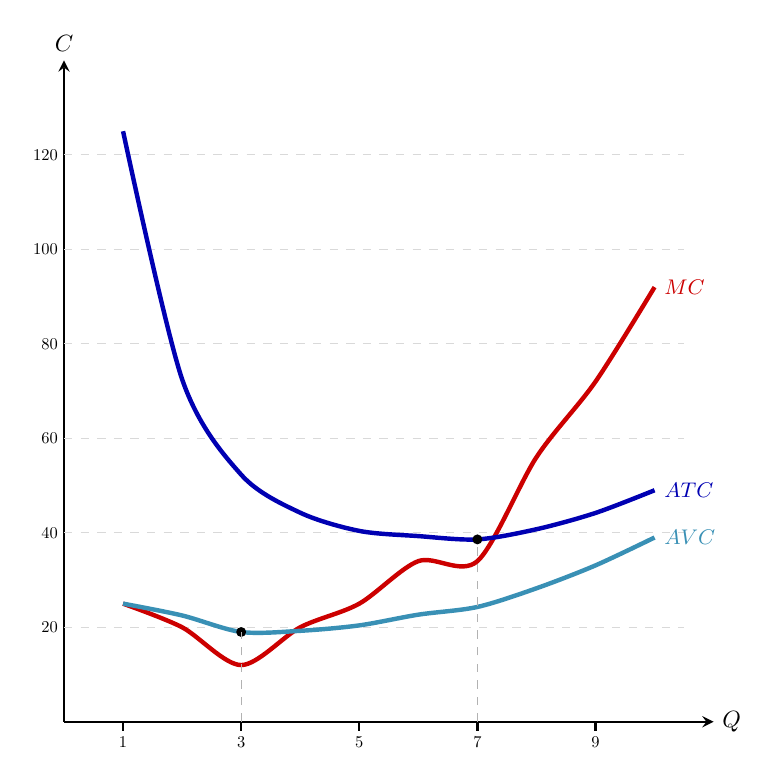
\begin{tikzpicture}[x=0.75cm, y=0.06cm, >=stealth, thick, every node/.style={scale=0.85}]
				% 坐标轴
				\draw[->] (0,0) -- (11,0) node[right] {$Q$};
				\draw[->] (0,0) -- (0,140) node[above] {$C$};
				
				% Y轴刻度（去噪声，仅保留关键梯度）
				\foreach \y in {20, 40, 60, 80, 100, 120} {
					\draw[gray!30, thin, dashed] (0,\y) -- (10.5,\y);
					\node[left, scale=0.7] at (0,\y) {\y};
				}
				
				% X轴刻度
				\foreach \x in {1, 3, 5, 7, 9} {
					\draw (\x, 0) -- (\x, -2) node[below, scale=0.7] {\x};
				}
				
				% 绘制 MC 曲线 (学术红)
				\draw[red!80!black, ultra thick] plot[smooth] coordinates {
					(1, 25) (2, 20) (3, 12) (4, 20) (5, 25) (6, 34) (7, 34) (8, 56) (9, 72) (10, 92)
				} node[right] {\small $MC$};
				
				% 绘制 AVC 曲线 (学术青)
				\draw[cyan!70!black, ultra thick] plot[smooth] coordinates {
					(1, 25) (2, 22.5) (3, 19) (4, 19.25) (5, 20.4) (6, 22.67) (7, 24.3) (8, 28.25) (9, 33.1) (10, 39)
				} node[right] {\small $AVC$};
				
				% 绘制 ATC 曲线 (深邃蓝)
				\draw[blue!70!black, ultra thick] plot[smooth] coordinates {
					(1, 125) (2, 72.5) (3, 52.3) (4, 44.25) (5, 40.4) (6, 39.3) (7, 38.6) (8, 40.75) (9, 44.2) (10, 49)
				} node[right] {\small $ATC$};
				
				% 标记最低点及交点 (纯线条/圆点，无冗余文字)
				\fill[black] (3,19) circle (1.8pt); 
				\fill[black] (7,38.6) circle (1.8pt);
				
				% 引导虚线
				\draw[dashed, gray!60, thin] (3,0) -- (3,19);
				\draw[dashed, gray!60, thin] (7,0) -- (7,38.6);
			\end{tikzpicture}
		\end{center}
		
		\newpage
		\item \textbf{一家厂商的固定生产成本为 5000 美元，边际生产成本为常数，500 美元。（1）总成本函数是什么？平均成本呢？（2）如果想使平均总成本最低，它应该选择非常大的产量还是比较小的产量？解释你的结论。}
		
		\textbf{答：}
		（1）由于边际生产成本为常数，根据边际成本与可变成本的关系，平均可变成本等于边际成本，即 $AVC = MC = 500$。
		总成本函数为固定成本与可变成本之和：
		\[ TC = FC + VC = 5000 + 500q \]
		平均总成本函数为总成本除以产量：
		\[ ATC = \frac{TC}{q} = \frac{5000}{q} + 500 \]
		
		（2）企业应该选择非常大的产量。
		由平均总成本函数可知，$ATC$ 由平均固定成本 $5000/q$ 和平均可变成本 $500$ 组成。随着产量 $q$ 的不断增加，平均固定成本趋于 0，从而使 $ATC$ 持续递减。当产量 $q$ 趋向于无穷大时，平均总成本将趋向于其下限值 500（即边际成本）。因此，为了实现平均总成本最低，厂商应尽可能扩大生产规模。
		
		\begin{center}
			\begin{tikzpicture}[x=0.04cm, y=0.005cm, >=stealth, thick, every node/.style={scale=0.85}]
				% 坐标轴
				\draw[->] (0,0) -- (130,0) node[right] {$q$};
				\draw[->] (0,0) -- (0,1100) node[above] {$C$};
				
				% 原点
				\node[below left] at (0,0) {$O$};
				
				% 渐近线 (MC=500)
				\draw[dashed, gray, thin] (0,500) node[left, text=black] {500} -- (120,500) node[below] {$MC=500$};
				
				% ATC 曲线: y = 5000/x + 500
				% x从9开始计算，最大y值为 5000/9+500 ≈ 1055，完美落在1100的轴距内
				\draw[blue, smooth, domain=9:115] plot (\x, {5000/\x + 500}) node[right] {$ATC$};
			\end{tikzpicture}
		\end{center}
		
		\item \textbf{假定某公司必须支付一笔固定数目的年金税，这笔费用与该公司的产量无关。（1）这项税收将如何影响公司的固定成本、边际成本和平均成本？（2）现假定该公司需支付一笔与其产量成比例的税收。那么，该税收又是如何影响公司的固定成本、边际成本以及平均成本的？}
		
		\textbf{答：}
		（1）由于年金税（设为 $T$）额度固定且与产量无关，属于固定成本。因此，这项税收将导致公司的固定成本 $FC$ 增加 $T$。
		边际成本 $MC$ 是总成本对产量的导数，由于定额税不随产量变动而变动，即 $\Delta T / \Delta q = 0$，故 $MC$ 保持不变。在平均成本方面，由于固定成本增加，平均总成本 $ATC$ 会整体向上位移，其变动量为 $T/q$。随着产量的增加，税收的摊薄效应显现。
		\[
		\begin{aligned}
			FC_2 &= FC_1 + T \\
			MC_2 &= MC_1 \\
			ATC_2 &= ATC_1 + \frac{T}{q}
		\end{aligned}
		\]
		
		（2）当税收与产量成比例（设单位税率为 $t$）时，它构成了公司的可变成本。此时，固定成本 $FC$ 不受该税收影响，保持不变。
		由于每增加一单位产量，企业必须多支付 $t$ 的税收，因此边际成本 $MC$ 和平均可变成本 $AVC$ 均会垂直向上平移 $t$。相应的，平均总成本 $ATC$ 也会同步向上平移 $t$。
		\[
		\begin{aligned}
			FC_2 &= FC_1 \\
			MC_2 &= MC_1 + t \\
			ATC_2 &= ATC_1 + t
		\end{aligned}
		\]
		
		\begin{center}
			\begin{tikzpicture}[x=0.7cm, y=0.7cm, >=stealth, thick, every node/.style={scale=0.8}]
				
				% ================= 左图：定额税 =================
				\begin{scope}[xshift=0cm]
					% 坐标轴
					\draw[->] (0,0) -- (4.8,0) node[right] {$q$};
					\draw[->] (0,0) -- (0,5) node[above] {$C$};
					\node[below left] at (0,0) {$O$};
					\node[above] at (2.4, 5) {（1）定额税：最低点向右上偏移};
					
					% MC线: y = x
					\draw[red, smooth, domain=0:4.5] plot (\x, {\x}) node[right] {$MC_1=MC_2$};
					
					% ATC1线: y = 1/x + 0.5x (最低点 q=1.41, C=1.41)
					\draw[blue, smooth, domain=0.35:4.5] plot (\x, {1/\x + 0.5*\x}) node[right] {$ATC_1$};
					
					% ATC2线: y = 2.5/x + 0.5x (最低点 q=2.24, C=2.24)
					\draw[cyan!80!blue, smooth, domain=0.7:4.5] plot (\x, {2.5/\x + 0.5*\x}) node[right] {$ATC_2$};
					
					% 最低点交点与辅助线
					\fill (1.41, 1.41) circle (1.5pt);
					\draw[dashed, gray, thin] (1.41,0) node[below, text=black] {$q_1$} -- (1.41,1.41);
					
					\fill (2.24, 2.24) circle (1.5pt);
					\draw[dashed, gray, thin] (2.24,0) node[below, text=black] {$q_2$} -- (2.24,2.24);
				\end{scope}
				
				% ================= 右图：比例税 =================
				\begin{scope}[xshift=5.8cm]
					% 坐标轴
					\draw[->] (0,0) -- (4.8,0) node[right] {$q$};
					\draw[->] (0,0) -- (0,5) node[above] {$C$};
					\node[below left] at (0,0) {$O$};
					\node[above] at (2.4, 5) {（2）比例税：最低点垂直向上平移};
					
					% MC1线: y = x
					\draw[red, smooth, domain=0:4] plot (\x, {\x}) node[right] {$MC_1$};
					
					% MC2线: y = x + 1.2
					\draw[red!60!purple, smooth, domain=0:3] plot (\x, {\x + 1.2}) node[right] {$MC_2$};
					
					% ATC1线: y = 1/x + 0.5x (最低点 q=1.41, C=1.41)
					\draw[blue, smooth, domain=0.35:4.5] plot (\x, {1/\x + 0.5*\x}) node[right] {$ATC_1$};
					
					% ATC2线: y = 1/x + 0.5x + 1.2 (最低点 q=1.41, C=2.61)
					\draw[cyan!80!blue, smooth, domain=0.35:4.2] plot (\x, {1/\x + 0.5*\x + 1.2}) node[right] {$ATC_2$};
					
					% 最低点交点与辅助线
					\fill (1.41, 1.41) circle (1.5pt);
					\fill (1.41, 2.61) circle (1.5pt);
					
					% 统一的 q1 辅助线，贯穿两个切点
					\draw[dashed, gray, thin] (1.41,0) node[below, text=black] {$q_1 = q_2$} -- (1.41,2.61);
					
					% 标记税收 t 的间距
					\draw[<->, gray, thin] (3.5, 2.04) -- (3.5, 3.24) node[midway, right] {$t$};
				\end{scope}
				
			\end{tikzpicture}
		\end{center}
		
		\item \textbf{最近一期《商业周刊》报道：“在汽车销售不景气时期，通用、福特和克莱斯勒认为，将汽车卖给出租公司的损失要比让工人暂时休息的成本小。这是因为汽车制造商现有的工会契约规定，即使工人无事可做也要给他们发工资。”这篇文章讨论的出售汽车的“损失”，是指会计利润还是指经济利润？这两种利润不同吗?简要说明为什么。}
		
		\textbf{答：}
		文章讨论的出售汽车的“损失”是指会计利润。
		会计利润与经济利润在成本界定上存在本质区别：
		
		（1）会计利润仅关注显性成本，即账面上实际发生的货币支出。文中提到的工人工资由于受到工会契约的法律约束，无论是否开工都必须支付，在会计核算中被视为必须扣除的营业成本。当售价低于包含这部分工资在内的总会计成本时，会计利润即为负，表现为“损失”。
		
		（2）经济利润则关注机会成本。对于厂商而言，既然契约规定必须支付这笔工资，那么在短期决策中，这笔支出属于沉没成本，其机会成本为零。在经济学逻辑下，只要出售汽车的收益能够覆盖除这笔沉没成本之外的其他变动成本（如材料、电力等），生产便是理性的。因此，从经济利润的角度看，这种“损失”可能并不存在，或者说这种选择实际上是实现了亏损最小化。
		
		\item \textbf{假定经济处于衰退期，且劳动力的成本下降了 50\%，人们预期劳动力成本将在目前水平上保持较长的时间。试用图表表示劳动和资本的相对价格变动对企业扩张路径的影响。}
		
		\textbf{答：}
		扩张路径反映了在不同产出水平下实现成本最小化的最优要素投入组合。当劳动力成本 $w$ 下降 50\% 而资本价格 $r$ 保持不变时，等成本线的斜率绝对值 $w/r$ 会相应减小，导致等成本线绕其纵轴（资本轴）的截距点向外旋转，变得更加平缓。
		
		根据成本最小化原则，均衡点必须满足边际技术替代率等于要素价格比（$MRTS_{LK} = w/r$）。由于劳动变得相对便宜，厂商会倾向于用劳动替代资本。在任意既定的产出水平下（如等产量线 $Q_1, Q_2$），成本最小化的最优切点将由原切点 $E_1, E_2$ 沿着等产量线向右下方移动至新切点 $E_1', E_2'$。
		
		连接原切点形成的初始扩张路径 $EP_1$，将向代表劳动的横轴方向发生旋转，形成新的扩张路径 $EP_2$。这在图形上表现为一条斜率更小的射线，深刻体现了企业生产过程向劳动密集型技术的系统性转型。
		
		\begin{center}
			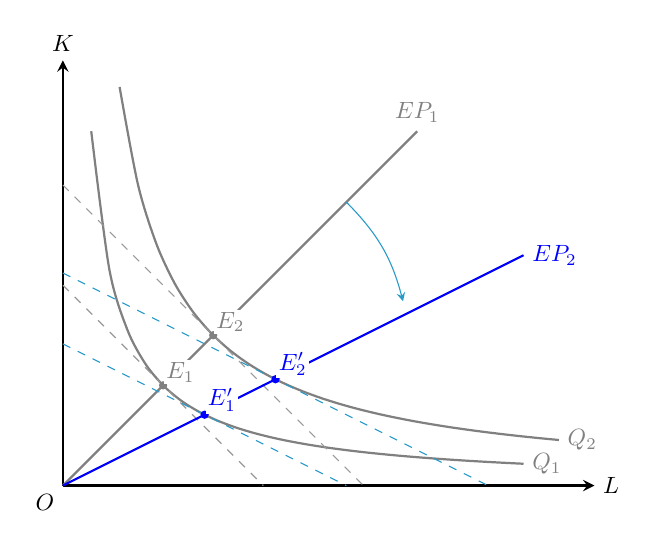
\begin{tikzpicture}[x=0.9cm, y=0.9cm, >=stealth, thick, every node/.style={scale=0.85}]
				% 坐标轴
				\draw[->] (0,0) -- (7.5,0) node[right] {$L$};
				\draw[->] (0,0) -- (0,6) node[above] {$K$};
				\node[below left] at (0,0) {$O$};
				
				% 等产量线 Q=KL (Q1=2, Q2=4.5)
				\draw[gray, smooth, domain=0.4:6.5] plot (\x, {2/\x}) node[right] {$Q_1$};
				\draw[gray, smooth, domain=0.8:7] plot (\x, {4.5/\x}) node[right] {$Q_2$};
				
				% 原始情况 (w/r = 1, 斜率为 -1)
				\draw[dashed, gray!80, thin] (0, 2.828) -- (2.828, 0); % Q1 对应的初始等成本线
				\draw[dashed, gray!80, thin] (0, 4.242) -- (4.242, 0); % Q2 对应的初始等成本线
				
				% 原始扩张路径 EP1 (K = L)
				\draw[gray, thick] (0,0) -- (5, 5) node[above] {$EP_1$};
				
				% 原始切点
				\fill[gray] (1.414, 1.414) circle (1.5pt) node[above right, fill=white, inner sep=1pt] {$E_1$};
				\fill[gray] (2.121, 2.121) circle (1.5pt) node[above right, fill=white, inner sep=1pt] {$E_2$};
				
				% 劳动力价格下降后 (w/r = 0.5, 斜率为 -0.5)
				\draw[dashed, cyan!80!black, thin] (0, 2) -- (4, 0); % Q1 对应的新等成本线
				\draw[dashed, cyan!80!black, thin] (0, 3) -- (6, 0); % Q2 对应的新等成本线
				
				% 新扩张路径 EP2 (K = 0.5L)
				\draw[blue, thick] (0,0) -- (6.5, 3.25) node[right] {$EP_2$};
				
				% 新切点
				\fill[blue] (2, 1) circle (1.5pt) node[above right, fill=white, inner sep=1pt] {$E_1'$};
				\fill[blue] (3, 1.5) circle (1.5pt) node[above right, fill=white, inner sep=1pt] {$E_2'$};
				
				% 旋转指示箭头 (从 EP1 指向 EP2)
				\draw[->, cyan!80!black, thin] (4, 4) to[bend left=15] (4.8, 2.6);
			\end{tikzpicture}
		\end{center}
		
		\item \textbf{从 A 地到 B 地的飞行成本为 50000 美元，每天有四趟航班，分别在上午 7 点、10 点，下午 1 点和 4 点。飞机容量为 240 个座位，每天第一班和最后一班都是满载的，而第二班和第三班只有一半座位坐满，计算每趟航班的平均成本。如果你是航空公司的咨询顾问，航空公司想知道它应该吸引哪一类顾客，是非高峰期顾客（乘坐中间两趟航班）还是高峰期顾客（乘坐第一趟和最后一趟航班），你的建议是什么？}
		
		\textbf{答：}
		对于第一趟和最后一趟（高峰期）航班而言，满载（240人）时的平均总成本为：
		\[
		\begin{aligned}
			ATC_{\text{高峰}} = \frac{50000}{240} \approx 208.33 \text{（美元）}
		\end{aligned}
		\]
		
		对于第二趟和第三趟（非高峰期）航班而言，半载（120人）时的平均总成本为：
		\[
		\begin{aligned}
			ATC_{\text{非高峰}} = \frac{50000}{120} \approx 416.67 \text{（美元）}
		\end{aligned}
		\]
		
		在经营策略上，作为咨询顾问，建议航空公司应该致力于吸引更多的非高峰期顾客。
		
		这是因为航班的单次飞行成本（50000 美元）在起飞前已大多转化为固定成本或沉没成本。对于尚有一半空座的中间两趟非高峰期航班（对应需求曲线 $D_1$）而言，在达到最大物理容量（240个座位）之前，额外搭载一名乘客的边际成本（$MC$）几乎为零。只要向非高峰期顾客收取的票价大于这极低的边际成本，就能为公司带来正的边际利润，从而摊薄目前高昂的平均成本。
		
		相反，高峰期航班（对应需求曲线 $D_2$）已经达到容量上限。此时边际成本曲线呈垂直形态，吸引更多乘客既无法实质性增加上座率，也无法带来额外收益。除非航空公司实行高峰期价格歧视以获取更多消费者剩余，否则在现有航班班次下，唯一的利润增长点在于填补非高峰期的闲置产能。
		
		\begin{center}
			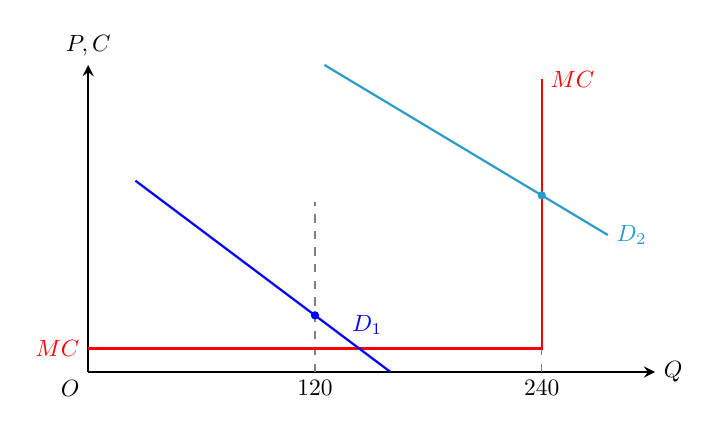
\begin{tikzpicture}[x=1.2cm, y=0.6cm, >=stealth, thick, every node/.style={scale=0.85}]
				% 坐标轴
				\draw[->] (0,0) -- (6,0) node[right] {$Q$};
				\draw[->] (0,0) -- (0,6.5) node[above] {$P, C$};
				\node[below left] at (0,0) {$O$};
				
				% 容量约束线 (Q_max = 240, 映射到 x=4.8)
				\draw[dashed, gray, thin] (4.8, 0) node[below, text=black] {$240$} -- (4.8, 5.5);
				
				% 非高峰期当前人数 (Q = 120, 映射到 x=2.4)
				\draw[dashed, gray, thin] (2.4, 0) node[below, text=black] {$120$} -- (2.4, 3.6);
				
				% L型边际成本曲线 (MC)
				\draw[red, thick] (0, 0.5) node[left] {$MC$} -- (4.8, 0.5) -- (4.8, 6.2) node[right] {$MC$};
				
				% 非高峰期需求曲线 (D1) 
				% 修正: domain最高取到3.2, 避免 y = 4.8 - 1.5*x 变成负数而穿透横轴
				\draw[blue, smooth, domain=0.5:3.2] plot (\x, {4.8 - 1.5*\x}) node[right,xshift=-20pt,yshift=20pt] {$D_1$};
				
				% 高峰期需求曲线 (D2)
				\draw[cyan!80!black, smooth, domain=2.5:5.5] plot (\x, {9.5 - 1.2*\x}) node[right] {$D_2$};
				
				% 均衡点标记
				\fill[blue] (2.4, 1.2) circle (1.5pt); % 非高峰期半载均衡点
				\fill[cyan!80!black] (4.8, 3.74) circle (1.5pt); % 高峰期满载均衡点
			\end{tikzpicture}
		\end{center}
		
		\newpage
		\item \textbf{你管理一家大规模生产发动机的工厂，通过在装配线上团队工作。生产技术由下列生产函数给出：$q = 5KL$。式中，$q$ 为每周生产出的发动机；$K$ 为装配线的数量；$L$ 为劳动团队的数量。租用一套装配线的每周租金 $r = 10000$ 美元，每个劳动团队的成本 $w = 5000$ 美元。发动机的成本为劳动和装配线成本之和，外加每台发动机的原材料成本 2000 美元。你的工厂安装了固定的 5 套装配线。\\（1）你的工厂的成本函数是什么？即生产 $q$ 台发动机需要多少成本？生产 $q$ 台发动机的平均成本和边际成本为多少？平均成本如何随 $q$ 的变动而变化？\\（2）生产 250 台发动机需投入多少个劳动团队？每台发动机的平均成本为多少？\\（3）如果要你为一新的生产能力提出建议。如果你想最小化每一产出下的总成本，那么新工厂的资本/劳动比率（$K/L$）应为多少？}
		
		\textbf{解：}
		（1）在短期内，资本固定为 $K = 5$。代入生产函数得 $q = 25L$，因此生产 $q$ 单位产量所需的劳动团队数量为 $L = \frac{q}{25}$。
		总成本（$TC$）由资本成本、劳动成本和原材料可变成本构成：
		\[
		\begin{aligned}
			TC &= rK + wL + 2000q \\
			&= 10000 \times 5 + 5000 \times \left(\frac{q}{25}\right) + 2000q \\
			&= 50000 + 2200q \ \text{（美元）}
		\end{aligned}
		\]
		平均成本（$ATC$）和边际成本（$MC$）分别为：
		\[
		\begin{aligned}
			ATC &= \frac{TC}{q} = \frac{50000}{q} + 2200 \\
			MC &= \frac{dTC}{dq} = 2200
		\end{aligned}
		\]
		随着产量 $q$ 的增加，固定成本被不断摊薄，平均成本将持续递减，并无限趋近于边际成本 2200 美元。
		
		（2）生产 250 台发动机所需的劳动团队数量为：
		\[
		\begin{aligned}
			L = \frac{250}{25} = 10 \text{（个）}
		\end{aligned}
		\]
		此时，每台发动机的平均成本为：
		\[
		\begin{aligned}
			ATC = \frac{50000}{250} + 2200 = 2400 \text{（美元）}
		\end{aligned}
		\]
		
		（3）在长期中，资本与劳动均可变。为了最小化总成本，企业应使要素的边际技术替代率等于要素价格比，即
		$$\frac{MP_L}{MP_K} = \frac{w}{r}$$
		已知生产函数 $q = 5KL$，则 $MP_L = 5K$，$MP_K = 5L$。代入最优条件：
		\[
		\begin{aligned}
			\frac{5K}{5L} = \frac{5000}{10000} \implies \frac{K}{L} = \frac{1}{2}
		\end{aligned}
		\]
		因此，新工厂的资本/劳动比率应设定为 $1/2$。无论目标产出是多少，维持这一要素投入比例始终能实现长期成本最小化。
		\newpage
		\item \textbf{某公司的短期总成本函数由等式 $TC = 200 + 55q$ 给出，式中，$TC$ 为总成本；$q$ 为总产出数量；两者均以千计。\\（1）该公司的固定成本是多少？\\（2）如果该公司生产了 100000 单位的产品，它的平均可变成本是多少？\\（3）生产的边际成本是多少？\\(4) 平均固定成本是多少?\\（5）假定该公司通过贷款扩大生产规模，其固定成本增加 50000 美元，但其可变成本降至每 1000 单位产品 45000 美元，利率 $i$ 也进入成本函数。利率每上升 1\%，成本增加 3000 美元。写出新的成本函数。}
		
		\textbf{解：}
		（1）由于 $q=0$ 时的成本即为固定成本，由函数可知固定成本 $FC = 200$（千美元），即 $200,000$ 美元。
		
		（2）当公司生产 100,000 单位产品时，由于变量 $q$ 以千计，此时 $q = 100$。
		总可变成本 $VC = 55q$，因此平均可变成本为：
		\[
		\begin{aligned}
			AVC = \frac{VC}{q} = 55 \text{（千美元）}
		\end{aligned}
		\]
		
		（3）生产的边际成本是对总成本函数求导：
		\[
		\begin{aligned}
			MC = \frac{dTC}{dq} = 55 \text{（千美元）}
		\end{aligned}
		\]
		
		（4）在 $q = 100$ 时的平均固定成本为：
		\[
		\begin{aligned}
			AFC = \frac{FC}{q} = \frac{200}{100} = 2 \text{（千美元）}
		\end{aligned}
		\]
		
		（5）贷款扩产后，固定成本从 200 增加到 250（增加 50千美元）；单位可变成本从 55 降至 45（千美元）。利率影响作为固定成本的一部分，可表示为 $3i$（由于利率上升1\%增加3千美元，设定 $i$ 以百分点计）。新的总成本函数为：
		\[
		\begin{aligned}
			TC = 250 + 45q + 3i
		\end{aligned}
		\]
		
		
		
		\item \textbf{某椅子生产商以 30 美元/小时的价格为其生产线雇佣劳动，并假定其机器设备的租金为 15 美元/小时。假定以任何劳动和机器设备的组合生产每把椅子都需 4 小时，如果该公司每使用 3 小时的劳动搭配 1 小时机器设备，它最小化了生产成本吗？如果是，请解释其原因；如果不是，怎样才能改善当前的境况呢？在图上画出等产量线和两条等成本线，其中一条为该厂商当前劳动和资本组合对应的等成本线，另一条为该厂商最优劳动和资本组合对应的等成本线。}
		
		\textbf{答：}
		该生产商目前的投入组合（3 小时劳动，1 小时机器）并未实现生产成本最小化。
		
		由题意可知，“以任何劳动和机器设备的组合生产每把椅子都需 4 小时”，这意味着劳动（$L$）和资本（$K$）在生产过程中是完全替代品。生产 1 把椅子的等产量线方程为 $L + K = 4$，其斜率的绝对值即边际技术替代率恒为 1（$MRTS = 1$）。
		
		考察要素市场的相对价格：
		\[
		\begin{aligned}
			\frac{w}{r} &= \frac{30}{15} = 2
		\end{aligned}
		\]
		由于 $$MRTS < \frac{w}{r}$$
		即 $1 < 2$，这表明市场要求用 2 单位资本去换取 1 单位劳动，但在生产技术上 1 单位资本就能完全替代 1 单位劳动。劳动的相对市场价格被高估，厂商处于技术上的比较劣势。
		
		为了改善境况并最小化成本，该厂商应彻底放弃雇佣劳动，转向全部使用机器设备，形成“角点解”。将产量目标 $L + K = 4$ 与非负约束结合，最优要素组合为 $L = 0, K = 4$。
		此时的成本节约效应如下：
		\[
		\begin{aligned}
			TC_A &= wL_A + rK_A = 30 \times 3 + 15 \times 1 = 105 \text{（美元）} \\
			TC_E &= wL_E + rK_E = 30 \times 0 + 15 \times 4 = 60 \text{（美元）}
		\end{aligned}
		\]
		通过调整至最优组合，该厂商成功节约了 45 美元的生产成本。
		
		\begin{center}
			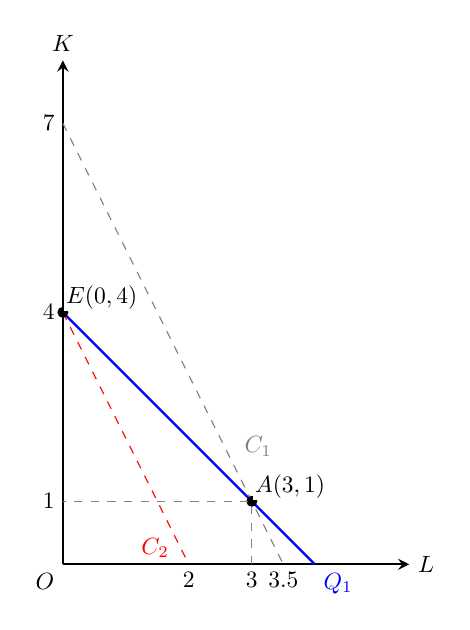
\begin{tikzpicture}[x=0.8cm, y=0.8cm, >=stealth, thick, every node/.style={scale=0.85}]
				% 坐标轴
				\draw[->] (0,0) -- (5.5,0) node[right] {$L$};
				\draw[->] (0,0) -- (0,8) node[above] {$K$};
				\node[below left] at (0,0) {$O$};
				
				% 等产量线 Q=1 (L+K=4)
				\draw[blue, smooth] (0, 4) -- (4, 0) node[below right] {$Q_1$};
				
				% 当前等成本线 C1: TC=105 (K = 7 - 2L)
				\draw[gray, dashed, thin] (0, 7) node[left, text=black] {$7$} -- (3.5, 0) node[below, text=black] {$3.5$} node[right,yshift=50pt,xshift=-20pt] {$C_1$};
				
				% 最优等成本线 C2: TC=60 (K = 4 - 2L)
				\draw[red, dashed, thin] (0, 4) node[left, text=black] {$4$} -- (2, 0) node[below, text=black] {$2$} node[left,xshift=-5pt,yshift=7pt] {$C_2$};
				
				% 当前组合点 A
				\fill (3, 1) circle (2pt) node[above right, fill=white, inner sep=1pt] {$A(3, 1)$};
				\draw[dashed, gray, thin] (3,0) node[below, text=black] {$3$} -- (3,1) -- (0,1) node[left, text=black] {$1$};
				
				% 最优角点解 E
				\fill (0, 4) circle (2pt) node[above right, fill=white, inner sep=1pt] {$E(0, 4)$};
			\end{tikzpicture}
		\end{center}
		
		
		
		\item \textbf{假定厂商的生产函数为 $q = 10L^{1/2}K^{1/2}$，单位劳动成本为 20 美元，单位资本成本为 80 美元。\\（1）厂商目前的产量为 100 单位，成本最小化的劳动和资本分别为 20 和 5。在图上用等产量线和等成本线表示出来。\\（2）厂商想将产量扩大为 140 单位，如果资本在短期固定，需要多少劳动？在图形上表示出来，并计算厂商新的成本。\\（3）在图形上表示出厂商在长期生产 140 单位产品的成本最小化劳动和资本投入。\\（4）如果边际技术替代率为 $K / L$，计算生产 140 单位产品的最优劳动和资本投入水平。}
		
		\textbf{答：}
		（1）当前产量 $q=100$，代入生产函数得 $100 = 10L^{1/2}K^{1/2}$，整理可得该产出水平下的等产量线方程为 $LK = 100$。
		已知当前投入为 $L=20, K=5$，此时最小化的总成本为：
		\[
		\begin{aligned}
			TC_1 &= 20 \times 20 + 80 \times 5 = 800 \text{（美元）}
		\end{aligned}
		\]
		对应的等成本线方程为 $20L + 80K = 800$。在图上，该状态对应等产量线 $Q_1$ 与等成本线 $C_1$ 相切的最优均衡点 $A$。
		
		（2）在短期内，资本要素不可变动，被锁定在当前水平 $K = 5$。若企业要将产量扩大至 140 单位，代入生产函数：
		\[
		\begin{aligned}
			140 &= 10L^{1/2}(5)^{1/2} \\
			14 &= \sqrt{5L} \implies 196 = 5L \implies L = 39.2
		\end{aligned}
		\]
		在短期扩张中，企业必须雇佣 39.2 单位劳动。此时新的总成本为：
		\[
		\begin{aligned}
			TC_2 &= 20 \times 39.2 + 80 \times 5 = 784 + 400 = 1184 \text{（美元）}
		\end{aligned}
		\]
		由于资本固定，这一非最优要素组合在图上表现为沿短期扩张路径$EP_S$移动至点 $C$。
		
		（4）在长期，要素投入比例可自由调整以实现成本最小化，均衡条件要求边际技术替代率等于要素相对价格（$MRTS = w/r$）。已知 $MRTS = K/L$：
		\[
		\begin{aligned}
			\frac{K}{L} &= \frac{20}{80} = \frac{1}{4} \implies L = 4K
		\end{aligned}
		\]
		将最优比例 $L = 4K$ 代入目标产量为 140 的等产量线方程（$LK = 196$）：
		\[
		\begin{aligned}
			(4K)K &= 196 \implies K^2 = 49 \\
			K &= 7, \quad L = 4 \times 7 = 28
		\end{aligned}
		\]（水平线
		因此，长期生产 140 单位产品的最优要素投入为 $L=28, K=7$。此时长期最小化总成本为：
		\[
		\begin{aligned}
			TC_3 &= 20 \times 28 + 80 \times 7 = 560 + 560 = 1120 \text{（美元）}
		\end{aligned}
		\]
		
		（3）综合上述分析，所有的成本变动与要素选择均映射于下图中。从原点出发的射线代表长期扩张路径（$EP_L$），点 $B$ 为长期重新实现效率优化的新切点。点 $C$ 则直观反映了短期内因要素刚性而偏离扩张路径所造成的效率损失，其对应的成本（1184 美元）显著高于长期均衡成本（1120 美元）。
		
		\begin{center}
			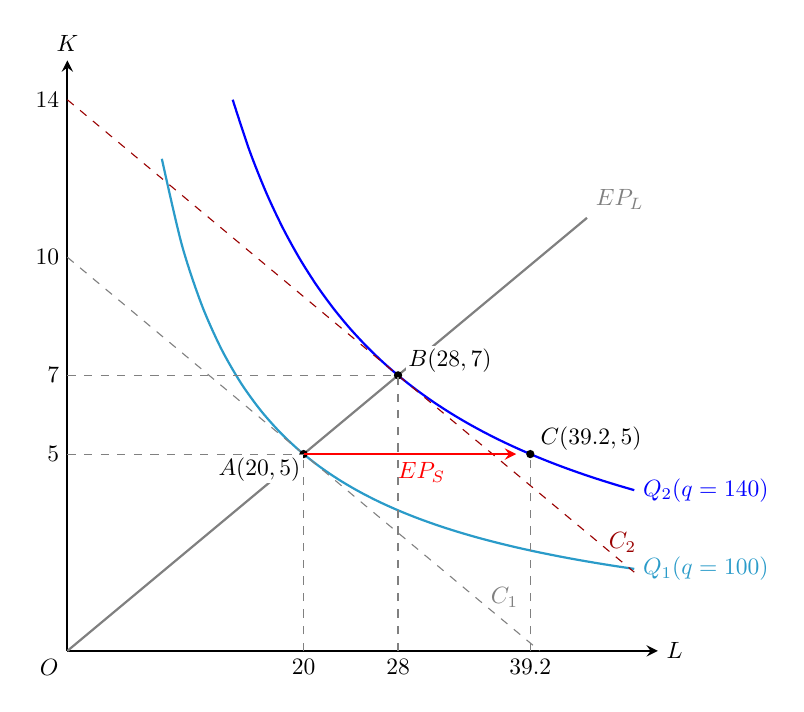
\begin{tikzpicture}[x=0.15cm, y=0.5cm, >=stealth, thick, every node/.style={scale=0.85}]
				% 坐标轴
				\draw[->] (0,0) -- (50,0) node[right] {$L$};
				\draw[->] (0,0) -- (0,15) node[above] {$K$};
				\node[below left] at (0,0) {$O$};
				
				% 等产量线 Q1 = 100 -> K = 100/L
				\draw[cyan!80!black, smooth, domain=8:48] plot (\x, {100/\x}) node[right] {$Q_1(q=100)$};
				
				% 等产量线 Q2 = 140 -> K = 196/L
				\draw[blue, smooth, domain=14:48] plot (\x, {196/\x}) node[right] {$Q_2(q=140)$};
				
				% 等成本线 C1 (过 A 点): TC = 800 -> K = 10 - 0.25L
				\draw[gray, dashed, thin] (0, 10) node[left, text=black] {$10$} -- (40, 0) node[above,xshift=-15pt,yshift=15pt] {$C_1$};
				
				% 等成本线 C2 (过 B 点): TC = 1120 -> K = 14 - 0.25L
				\draw[red!60!black, dashed, thin] (0, 14) node[left, text=black] {$14$} -- (48, 2) node[above,xshift=-5pt,yshift=5pt] {$C_2$};
				
				% 长期扩张路径 EP_L (K = 0.25L)
				\draw[gray, thick] (0,0) -- (44, 11) node[above right] {$EP_L$};
				
				% A 点 (20, 5)
				\fill (20, 5) circle (1.5pt) node[below left, fill=white, inner sep=1pt] {$A(20,5)$};
				
				% B 点 (28, 7)
				\fill (28, 7) circle (1.5pt) node[above right, fill=white, inner sep=1pt,xshift=3pt] {$B(28,7)$};
				
				% C 点 (39.2, 5)
				\fill (39.2, 5) circle (1.5pt) node[above right, fill=white, inner sep=1pt,xshift=3pt] {$C(39.2,5)$};
				
				% 短期扩张路径 EP_S (K=5 的水平线)
				\draw[->, red, thick] (20, 5) -- (38, 5) node[midway, below,xshift=5pt] {$EP_S$};
				
				% 辅助投影线
				\draw[dashed, gray, thin] (0, 5) node[left, text=black] {$5$} -- (20, 5);
				\draw[dashed, gray, thin] (0, 7) node[left, text=black] {$7$} -- (28, 7);
				\draw[dashed, gray, thin] (20, 0) node[below, text=black] {$20$} -- (20, 5);
				\draw[dashed, gray, thin] (28, 0) node[below, text=black] {$28$} -- (28, 7);
				\draw[dashed, gray, thin] (39.2, 0) node[below, text=black] {$39.2$} -- (39.2, 5);
			\end{tikzpicture}
		\end{center}
		
		\item \textbf{某计算机公司的成本函数将其生产的平均成本（$AC$）与累积的计算机产量（$Q$，以千计）和每年所制造的计算机千台数表示的工厂规模（$q$，范围在 10000～50000 台）联系在一起，其关系式如下：
			\[
			AC = 10 - 0.1Q + 0.3q
			\]
			（1）是否存在学习曲线效应？\\
			（2）是否存在规模经济或规模不经济？\\
			（3）从公司创立以来，共生产了 40000 台计算机，且今年生产了 10000 台。下一年度，公司打算将其生产扩大到 12000 台。公司的平均生产成本会上升还是下降？请解释。}
		
		\textbf{解：}
		（1）存在学习曲线效应。
		学习曲线反映的是企业的平均生产成本随着历史累积产量的增加而下降的现象。对平均成本函数求关于累积产量 $Q$ 的偏导数可得：
		\[
		\begin{aligned}
			\frac{\partial AC}{\partial Q} = -0.1 < 0
		\end{aligned}
		\]
		这表明，在当前生产规模 $q$ 给定的情况下，随着累积产量 $Q$ 的增加，平均成本呈现严格递减的趋势，印证了学习曲线效应的存在。
		
		（2）存在规模不经济。
		规模经济的判定取决于当期边际成本（$MC$）与平均成本（$AC$）的相对大小关系（即成本产出弹性 $E_c = MC/AC$）。
		已知当期总成本 $TC = AC \cdot q = 10q - 0.1Qq + 0.3q^2$，对其求当期产量 $q$ 的导数可得边际成本：
		\[
		\begin{aligned}
			MC = \frac{\partial TC}{\partial q} = 10 - 0.1Q + 0.6q
		\end{aligned}
		\]
		将边际成本与平均成本进行比较：
		\[
		\begin{aligned}
			MC - AC &= (10 - 0.1Q + 0.6q) - (10 - 0.1Q + 0.3q) \\
			&= 0.3q
		\end{aligned}
		\]
		由于工厂的实际产出 $q > 0$，因此必定有 $MC > AC$，即成本产出弹性 $E_c > 1$。这说明生产扩张带来的边际成本增量高于当前的平均成本，存在规模不经济。
		
		（3）公司的平均生产成本会下降。
		根据题意，$Q$ 和 $q$ 的单位均为千台。
		今年，公司的累积产量为 $Q_1 = 40$，当期产量为 $q_1 = 10$。今年的平均成本为：
		\[
		\begin{aligned}
			AC_1 = 10 - 0.1 \times 40 + 0.3 \times 10 = 10 - 4 + 3 = 9 \text{（千美元/千台）}
		\end{aligned}
		\]
		明年初，累积产量变为 $Q_2 = 40 + 10 = 50$。明年计划的当期产量为 $q_2 = 12$。明年的预期平均成本为：
		\[
		\begin{aligned}
			AC_2 = 10 - 0.1 \times 50 + 0.3 \times 12 = 10 - 5 + 3.6 = 8.6 \text{（千美元/千台）}
		\end{aligned}
		\]
		尽管扩大当期规模带来了规模不经济（导致单位成本承受了 $0.6$ 的上行压力），但由于这一年间积累了 10000 台的生产经验，强大的学习曲线效应（带来了 $1.0$ 的下行拉力）抵消并主导了成本走向，最终使平均成本由 9 下降至 8.6。
		
		\item \textbf{假定某行业的长期总成本函数为三次方程：$TC = a + bq + cq^2 + dq^3$。证明（用微积分）总成本函数至少在 $a$、$b$、$c$、$d$ 四个参数取某些值时体现为 U 形平均成本曲线。}
		
		\textbf{证明：}
		对于长期的 U 形平均成本（$AC$）曲线，我们可以通过微积分设定相关的约束条件来推导其参数特性。
		
		首先，在长期中所有生产要素都是可变的，不存在固定成本，因此当 $q=0$ 时 $TC=0$，这意味着 $a = 0$。
		此时，长期平均成本函数为：
		\[
		\begin{aligned}
			AC = \frac{TC}{q} = b + cq + dq^2
		\end{aligned}
		\]
		要使该曲线呈现标准的 U 形特征，必须满足以下三个微积分与经济学条件：
		第一，曲线存在一个极小值点，即二阶导数必须大于零：
		\[
		\begin{aligned}
			\frac{d^2 AC}{dq^2} = 2d > 0 \implies d > 0
		\end{aligned}
		\]
		第二，曲线的极小值点必须位于第一象限（产出 $q > 0$）：
		令一阶导数为零：
		\[
		\begin{aligned}
			\frac{dAC}{dq} = c + 2dq = 0 \implies q = -\frac{c}{2d}
		\end{aligned}
		\]
		由于 $d > 0$ 且极值点 $q > 0$，可推知 $c < 0$。
		
		第三，在极小值点处，平均成本不仅要最小化，且必须在经济学上是有意义的正值（$AC_{min} > 0$）：
		将 $q$ 代入平均成本函数：
		\[
		\begin{aligned}
			AC_{min} = b + c\left(-\frac{c}{2d}\right) + d\left(-\frac{c}{2d}\right)^2 = b - \frac{c^2}{4d} > 0
		\end{aligned}
		\]
		这就要求
		$$b > \frac{c^2}{4d}$$
		因为 $c^2 > 0$ 且 $d > 0$，所以 $b$ 必须严格大于 $0$。
		
		第四，（补充条件）为了保证在所有产出水平上边际成本 $MC > 0$。
		边际成本函数为 $MC = b + 2cq + 3dq^2$。其最小化产出点位于 $$q = -\frac{c}{3d}$$将此代入 $MC$ 函数并要求其最小值为正：
		\[
		\begin{aligned}
			MC_{min} = b - \frac{c^2}{3d} > 0 \implies 3bd > c^2
		\end{aligned}
		\]
		由于 $3bd > c^2$ 的条件比 $4bd > c^2$ 更为严格，因此只要满足前者即可。
		
		\textbf{举例：已知某厂商的成本函数参数设定为 $a=0, b=1, c=-1, d=1$，试推导其总成本、平均成本与边际成本函数，并绘制相应的成本曲线模型。}
		
		\textbf{答：}
		该参数设定满足 $d>0, c<0$ 且 $3bd > c^2$（即 $3 > 1$）的常规三次成本函数条件。根据参数，总成本函数为：
		\[
		\begin{aligned}
			TC &= q - q^2 + q^3
		\end{aligned}
		\]
		进一步求得平均成本函数 $AC = \frac{TC}{q}$ 为：
		\[
		\begin{aligned}
			AC &= 1 - q + q^2
		\end{aligned}
		\]
		对平均成本求导并令其为零，可得在 $q = 1/2$ 处 $AC$ 达到最低点，此时 $AC_{\min} = 3/4$。
		
		同时，对总成本求导可得边际成本函数：
		\[
		\begin{aligned}
			MC &= \frac{\mathrm{d}TC}{\mathrm{d}q} = 1 - 2q + 3q^2
		\end{aligned}
		\]
		同理，可知在 $q = 1/3$ 处 $MC$ 达到最低点，此时 $MC_{\min} = 2/3$。
		
		如下图所示，边际成本 $MC$ 曲线精准地从下方穿过了平均成本 $AC$ 曲线的最低点，构成了经典的长期 U 形成本几何模型。
		
		\begin{center}
			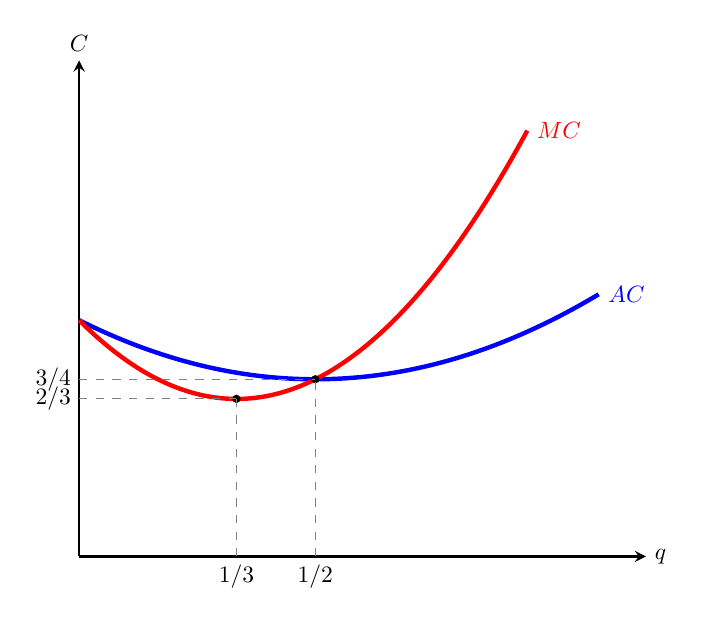
\begin{tikzpicture}[x=6cm, y=3cm, >=stealth, thick, every node/.style={scale=0.85}]
				% 坐标轴
				\draw[->] (0,0) -- (1.2,0) node[right] {$q$};
				\draw[->] (0,0) -- (0,2.1) node[above] {$C$};
				
				% 曲线绘制 (精确对应的代数方程)
				\draw[blue, ultra thick, domain=0:1.1, samples=100] plot (\x, {1 - \x + \x*\x}) node[right] {$AC$};
				\draw[red, ultra thick, domain=0:0.95, samples=100] plot (\x, {1 - 2*\x + 3*\x*\x}) node[right] {$MC$};
				
				% 关键点计算
				\fill[black] (0.5, 0.75) circle (1.5pt);
				\fill[black] (0.333, 0.667) circle (1.5pt);
				
				% AC 最低点辅助线
				\draw[dashed, gray, thin] (0.5, 0) node[below, black] {$1/2$} -- (0.5, 0.75);
				\draw[dashed, gray, thin] (0, 0.75) node[left, black] {$3/4$} -- (0.5, 0.75);
				
				% MC 最低点辅助线
				\draw[dashed, gray, thin] (0.333, 0) node[below, black] {$1/3$} -- (0.333, 0.667);
				\draw[dashed, gray, thin] (0, 0.667) node[left, black] {$2/3$} -- (0.333, 0.667);
			\end{tikzpicture}
		\end{center}
		\newpage
		\item \textbf{某计算机公司以同样的厂房和劳动生产硬件和软件。生产计算机处理器 $H$ 和软件 $S$ 的总成本由下式给出：$TC = aH + bS - cHS$，式中，$a$、$b$ 和 $c$ 均为正数。该总成本函数是否存在规模经济或规模不经济？是否存在范围经济或范围不经济？}
		
		\textbf{答：}
		首先，分别求出生产硬件和软件的边际成本：
		\[
		\begin{aligned}
			MC_H &= \frac{\partial TC}{\partial H} = a - cS \\
			MC_S &= \frac{\partial TC}{\partial S} = b - cH
		\end{aligned}
		\]
		
		关于规模经济。在多产品联合生产的环境下，规模经济指数定义为总成本与各项产出的边际成本之和的比例：
		\[
		\begin{aligned}
			S_{H, S} &= \frac{TC(H, S)}{H \cdot MC_H + S \cdot MC_S} \\
			&= \frac{aH + bS - cHS}{H(a - cS) + S(b - cH)} \\
			&= \frac{aH + bS - cHS}{aH + bS - 2cHS}
		\end{aligned}
		\]
		由于 $a$、$b$、$c$、$H$、$S$ 均为正数，交叉影响项 $cHS > 0$。分母比分子小了一个正向值 $cHS$，必然存在 $S_{H, S} > 1$。这说明该公司在联合生产硬件和软件时存在显著的规模经济。进一步考查单一产品专业化生产的规模经济指数（以硬件为例，将软件产出设为 $0$）：
		\[
		\begin{aligned}
			S_H &= \frac{TC(H, S) - TC(0, S)}{H \cdot MC_H} = \frac{(aH + bS - cHS) - bS}{H(a - cS)} = 1
		\end{aligned}
		\]
		同理可得 $S_S = 1$。这表明在此成本函数设定下，单一产品的自身生产技术表现为规模报酬不变，公司整体的规模经济完全来源于多产品的联合生产过程。
		
		关于范围经济。范围经济衡量的是多个企业分别专业化生产各项产品的总成本与单一企业联合生产所有产品总成本的差异程度。其指数定义为：
		\[
		\begin{aligned}
			SC &= \frac{TC(H, 0) + TC(0, S) - TC(H, S)}{TC(H, S)} \\
			&= \frac{aH + bS - (aH + bS - cHS)}{TC(H, S)} \\
			&= \frac{cHS}{TC(H, S)}
		\end{aligned}
		\]
		由于 $c > 0$ 且各项产出均为正，分子交叉项 $cHS > 0$，而总成本 $TC$ 必然大于 $0$。因此推导出 $SC > 0$。这充分证明了该成本函数存在明显的范围经济，即共享厂房和劳动进行软硬件联合生产的成本，严格低于单独设厂分别专业化生产软硬件的成本之和。
		
		\newpage
		\item \textbf{第15题：分析Jacob Viner关于长期平均成本（LAC）曲线与短期平均成本（SAC）曲线相切于各SAC曲线最低点的要求是否合理，并加以推导与作图说明。}
		
		\textbf{答：}
		完全支持画图员的观点，Jacob Viner 的要求在数学与几何上均不可能实现（除非在规模报酬不变的特殊前提下，即 LAC 曲线为绝对水平线）。短期内，由于存在固定生产要素，受边际报酬递减规律约束，每条代表特定工厂规模的短期平均成本（SAC）曲线均呈 U 形。而在长期中，厂商可以自由调整所有要素以实现特定产量下的成本最小化。
		
		长期平均成本（LAC）曲线在本质上是所有可能 SAC 曲线的下包络线，这一性质由包络线定理严格保证。它代表了厂商在长期内为每一个产量水平所能选择的最优工厂规模的最低平均成本集合。从几何映射来看，由于 LAC 曲线是下包络线，它只能与每条 SAC 曲线相切一次，且绝不相交。
		
		在规模经济阶段（即 LAC 曲线处于下降段），切点必然位于对应最优工厂 SAC 曲线最低点的左侧，因为此时 SAC 曲线在切点处也必须具有负斜率以满足相切的代数条件。同理，在规模不经济阶段（LAC 曲线处于上升段），切点必然位于 SAC 曲线最低点的右侧。只有在长期平均成本的唯一最低点处，由于切线斜率为零，SAC 曲线的最底端才会与 LAC 曲线精确相切。任何试图令下降或上升段的 SAC 最低点与 LAC 相切的尝试，在数学上必然导致 SAC 曲线穿透并低于 LAC 曲线，这直接推翻了下包络线的根本定义。
		
		\begin{center}
			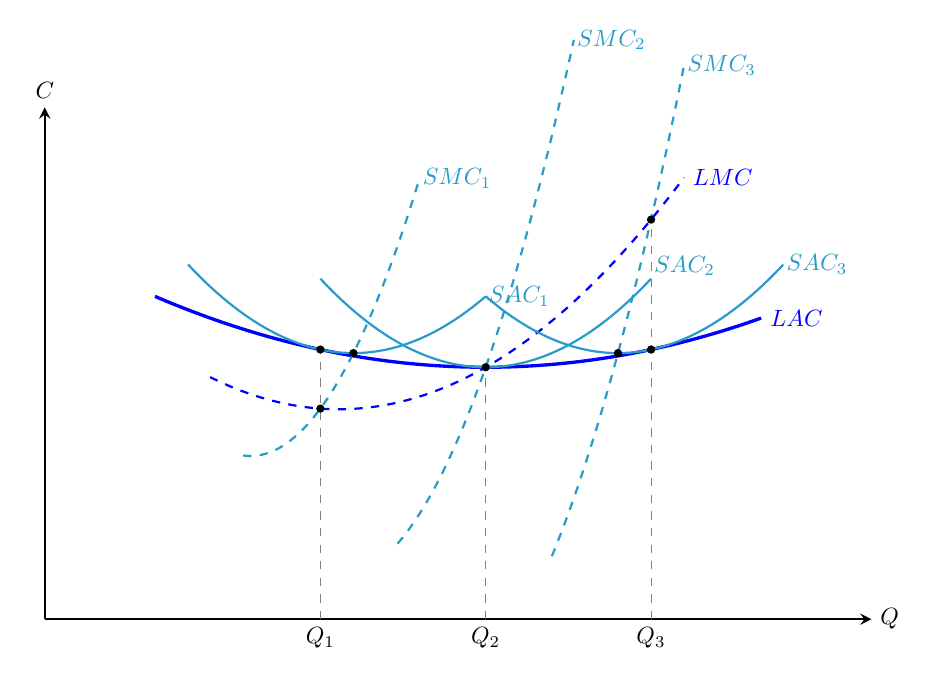
\begin{tikzpicture}[x=1.4cm, y=1.0cm, >=stealth, thick, every node/.style={scale=0.85}]
				% 坐标轴
				\draw[->] (0,0) -- (7.5,0) node[right] {$Q$};
				\draw[->] (0,0) -- (0,6.5) node[above] {$C$};
				
				% 纯代数推导的函数图像：完美保证相切与交点几何性质
				% LAC = 0.1*(x-4)^2 + 3.2
				% LMC = 0.3*x^2 - 1.6*x + 4.8
				\draw[blue, very thick, domain=1:6.5, samples=100] plot (\x, {0.1*(\x-4)^2 + 3.2}) node[right] {$LAC$};
				\draw[blue, dashed, domain=1.5:5.8, samples=100] plot (\x, {0.3*\x^2 - 1.6*\x + 4.8}) node[right] {$LMC$};
				
				% SAC1: Tangent at x=2.5, Min at x=2.8
				% SAC1 = 0.5*(x-2.8)^2 + 3.38
				% SMC1 = 1.5*x^2 - 5.6*x + 7.3
				% 严格限制 domain 防止 SMC 溢出
				\draw[cyan!80!black, thick, domain=1.3:4.0, samples=100] plot (\x, {0.5*(\x-2.8)^2 + 3.38}) node[right, fill=white, inner sep=1pt] {$SAC_1$};
				\draw[cyan!80!black, dashed, domain=1.8:3.4, samples=100] plot (\x, {1.5*\x^2 - 5.6*\x + 7.3}) node[right, fill=white, inner sep=1pt] {$SMC_1$};
				
				% SAC2: Tangent and Min at x=4
				% SAC2 = 0.5*(x-4)^2 + 3.2
				% SMC2 = 1.5*x^2 - 8*x + 11.2
				\draw[cyan!80!black, thick, domain=2.5:5.5, samples=100] plot (\x, {0.5*(\x-4)^2 + 3.2}) node[above right, fill=white, inner sep=1pt] {$SAC_2$};
				\draw[cyan!80!black, dashed, domain=3.2:4.8, samples=100] plot (\x, {1.5*\x^2 - 8*\x + 11.2}) node[right, fill=white, inner sep=1pt] {$SMC_2$};
				
				% SAC3: Tangent at x=5.5, Min at x=5.2
				% SAC3 = 0.5*(x-5.2)^2 + 3.38
				% SMC3 = 1.5*x^2 - 10.4*x + 16.9
				% 严格限制 domain 防止 SMC3 高度溢出
				\draw[cyan!80!black, thick, domain=4.0:6.7, samples=100] plot (\x, {0.5*(\x-5.2)^2 + 3.38}) node[right, fill=white, inner sep=1pt] {$SAC_3$};
				\draw[cyan!80!black, dashed, domain=4.6:5.8, samples=100] plot (\x, {1.5*\x^2 - 10.4*\x + 16.9}) node[right, fill=white, inner sep=1pt] {$SMC_3$};
				
				% 辅助线与坐标投影 (避开奇点，使用细虚线防干扰)
				\draw[dashed, gray, thin] (2.5,0) node[below, text=black] {$Q_1$} -- (2.5, 3.425);
				\draw[dashed, gray, thin] (4,0) node[below, text=black] {$Q_2$} -- (4, 3.2);
				\draw[dashed, gray, thin] (5.5,0) node[below, text=black] {$Q_3$} -- (5.5, 5.075);
				
				% 关键点标注（使用代数坐标确保完美压线）
				\fill (2.5, 3.425) circle (1.5pt); % SAC1 切点
				\fill (2.8, 3.38) circle (1.5pt);  % SAC1 最低点
				\fill (2.5, 2.675) circle (1.5pt); % LMC 与 SMC1 交点
				
				\fill (4, 3.2) circle (1.5pt);     % SAC2/LAC 切点兼最低点
				
				\fill (5.5, 3.425) circle (1.5pt); % SAC3 切点
				\fill (5.2, 3.38) circle (1.5pt);  % SAC3 最低点
				\fill (5.5, 5.075) circle (1.5pt); % LMC 与 SMC3 交点
			\end{tikzpicture}
		\end{center}
		\newpage
		\item \textbf{第16题：已知某停车场建设项目的产量固定为1000个停车位，土地（$T$）为固定要素。水泥价格 $P_C=4000$ 美元/英亩，劳动价格 $P_L=12$ 美元/小时。当前要素配置下，水泥的边际产量 $MP_C=50$，劳动的边际产量 $MP_L=4$。问厂商是否实现了成本最小化？若未实现，应如何调整要素投入比例？}
		
		\textbf{答：}
		该厂商并未实现成本最小化。在既定产量且存在固定要素的短期生产决策中，实现可变成本最小化的一阶必要条件是：厂商在每一种可变生产要素上花费的最后一单位货币，所带来的边际产量必须严格相等。
		
		根据已知参数对当前的要素边际生产率进行代数核算，劳动与水泥的单位货币边际收益分别为：
		\[
		\begin{aligned}
			\frac{MP_L}{P_L} &= \frac{4}{12} \approx 0.3333 \\
			\frac{MP_C}{P_C} &= \frac{50}{4000} = 0.0125
		\end{aligned}
		\]
		
		核算结果显示
		
		$$\frac{MP_L}{P_L} \gg \frac{MP_C}{P_C}$$
		
		这意味着在当前的要素组合下，劳动的边际性价比显著优于水泥。具体而言，厂商每增加 $1$ 美元的劳动投入可额外获得约 $0.33$ 个停车位的产出，而同等额度资金若投入水泥，仅能带来 $0.0125$ 个停车位的边际贡献。
		
		为纠正这一无效率的要素配置状态并压缩总成本，厂商必须启动要素替代机制。核心调整策略是：在保持 $1000$ 个停车位总产量绝对不变的前提下，持续减少水泥的投入量，并将节约的资金用于增加劳动雇佣量。依据微观经济学中的边际报酬递减规律，随着劳动投入的不断增加，其边际产量 $MP_L$ 将随之内生性下降；反之，水泥投入的缩减将促使其边际产量 $MP_C$ 逐步回升。厂商应维持这一动态替代过程，直至两者的单位货币边际产量完全趋同，即等产量线与等成本线在几何上实现完美相切，方可达到该产量下的成本最小化均衡解。
	\end{enumerate}
	
	\newpage
	\section{第7章附录}
	\begin{enumerate}[label=\textbf{\arabic*.}, leftmargin=*]
		\item \textbf{在下列生产函数中，哪些显示出规模报酬递增、不变和递减？\\(1) $F(K, L) = K^2 L$；\\(2) $F(K, L) = 10K + 5L$；\\(3) $F(K, L) = (KL)^{0.5}$}
		
		\textbf{答：}
		判断规模报酬属性，需考察所有生产要素等比例增加 $\lambda$ 倍（$\lambda > 1$）时，产出水平的变化情况。若 $F(\lambda K, \lambda L) > \lambda F(K, L)$ 为递增；相等为不变；小于则为递减。
		
		（1）对于 $F(K, L) = K^2 L$：
		\[
		\begin{aligned}
			F(\lambda K, \lambda L) &= (\lambda K)^2 (\lambda L) \\
			&= \lambda^3 K^2 L \\
			&= \lambda^3 F(K, L) > \lambda F(K, L)
		\end{aligned}
		\]
		该生产函数表现为规模报酬递增。
		
		（2）对于 $F(K, L) = 10K + 5L$：
		\[
		\begin{aligned}
			F(\lambda K, \lambda L) &= 10(\lambda K) + 5(\lambda L) \\
			&= \lambda (10K + 5L) \\
			&= \lambda F(K, L)
		\end{aligned}
		\]
		该生产函数表现为规模报酬不变。
		
		（3）对于 $F(K, L) = (KL)^{0.5}$：
		\[
		\begin{aligned}
			F(\lambda K, \lambda L) &= (\lambda K \cdot \lambda L)^{0.5} \\
			&= (\lambda^2 KL)^{0.5} \\
			&= \lambda (KL)^{0.5} = \lambda F(K, L)
		\end{aligned}
		\]
		该生产函数表现为规模报酬不变。
		
		\item \textbf{某产品的生产函数由 $q = 100KL$ 给出。若资本价格为 120 美元/天，而劳动价格为 30 美元/天。生产 1000 单位产出的最小成本是多少？}
		
		\textbf{答：}
		已知劳动与资本的边际产量分别为 $MP_L = 100K$，$MP_K = 100L$。
		成本最小化的一阶条件要求边际技术替代率等于要素价格比：
		\[
		\begin{aligned}
			MRTS &= \frac{MP_L}{MP_K} = \frac{w}{r} \\
			\frac{100K}{100L} &= \frac{30}{120} \implies L = 4K
		\end{aligned}
		\]
		将 $L = 4K$ 代入目标产量的生产函数 $q = 100KL$ 中：
		\[
		\begin{aligned}
			1000 &= 100K(4K) \\
			400K^2 &= 1000 \implies K \approx 1.58
		\end{aligned}
		\]
		由此可得最优劳动投入量 $L \approx 6.32$。
		最小化总成本为：
		\[
		\begin{aligned}
			TC &= wL + rK \\
			&= 30 \times 6.32 + 120 \times 1.58 \\
			&\approx 379.2 \text{（美元）}
		\end{aligned}
		\]
		
		\item \textbf{假定某生产函数由 $F(K, L) = KL^2$ 给出，资本价格为 10 美元，劳动力价格为 15 美元，什么是生产既定产出的成本最小化的资本和劳动的组合？}
		
		\textbf{答：}
		已知要素价格 $r=10$，$w=15$。给定产出约束为 $Q_0$。为求解成本最小化的要素组合，构建拉格朗日函数如下：
		\[
		\begin{aligned}
			\mathcal{L}(K, L, \lambda) &= 10K + 15L - \lambda (KL^2 - Q_0)
		\end{aligned}
		\]
		极值的一阶条件为：
		\[
		\begin{aligned}
			\frac{\partial \mathcal{L}}{\partial K} &= 10 - \lambda L^2 = 0 \\
			\frac{\partial \mathcal{L}}{\partial L} &= 15 - 2\lambda KL = 0
		\end{aligned}
		\]
		将上述两式相除消去拉格朗日乘数 $\lambda$，可得要素的边际技术替代率等于要素价格之比：
		\[
		\begin{aligned}
			\frac{10}{15} &= \frac{L^2}{2KL} \\
			\frac{2}{3} &= \frac{L}{2K} \implies \frac{K}{L} = \frac{3}{4}
		\end{aligned}
		\]
		因此，生产既定产出的成本最小化要素组合需满足资本与劳动之比为 $3:4$。
		
		如下图所示，当要素组合比例满足上述条件时，等成本线与等产量线实现相切，达到给定产量下的成本最小值。
		
		\begin{center}
			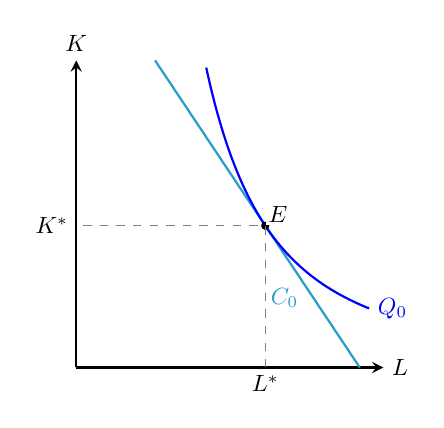
\begin{tikzpicture}[x=0.6cm, y=0.6cm, >=stealth, thick, every node/.style={scale=0.85}]
				% 坐标轴 (高度截断至6.5，大幅节省垂直版面)
				\draw[->] (0,0) -- (6.5,0) node[right] {$L$};
				\draw[->] (0,0) -- (0,6.5) node[above] {$K$};
				
				% 等成本线 C = 10K + 15L (局部截断：不再画到 K=9 的截距，只画 L=1.667 到 L=6 的核心区间)
				\draw[cyan!80!black] (1.667, 6.5) -- (6,0) node[pos=0.75, left,xshift=-3pt,yshift=-3pt, fill=white, inner sep=1pt] {$C_0$};
				
				% 等产量线 K = 48 / L^2 (同步限制定义域，防止曲线向上冲出坐标轴)
				\draw[blue, smooth, domain=2.75:6.2, samples=100] plot (\x, {48/(\x*\x)}) node[right] {$Q_0$};
				
				% 切点与辅助线
				\fill[black] (4,3) circle (1.5pt) node[above right, fill=white, inner sep=1pt] {$E$};
				\draw[dashed, gray, thin] (4,0) node[below, black] {$L^*$} -- (4,3) -- (0,3) node[left, black] {$K^*$};
			\end{tikzpicture}
		\end{center}
		
		\newpage
		\item \textbf{假定波莉制衣公司生产的轻型大衣的生产过程由下列生产函数给出：$q = 10K^{0.8}(L - 40)^{0.2}$。其中，$q$ 是大衣的生产数量，$K$ 是机器工作小时数，$L$ 是劳动小时数量。除资本和劳动外，每件大衣还需 10 美元原材料。（1）将成本最小化，推导出对 $K$ 和 $L$ 的成本最小化需求函数。再推导出总成本函数。（2）已知熟练工人工资为 32 美元/小时，机器租金为 64 美元/小时。作为 $q$ 的函数的总成本为多少？该技术呈现出规模递减、不变还是递增？（3）若每周生产 2000 件大衣，需雇佣多少劳动力和机器（每周按 40 小时计）？此产出水平的边际成本和平均成本各为多少？}
		
		\textbf{答：}
		（1）为实现成本最小化，首先计算资本与劳动的边际产量，并令边际技术替代率等于要素价格比：
		\[
		\begin{aligned}
			MP_L = 2 \left( \frac{K}{L - 40} \right)^{0.8}, \quad MP_K = 8 \left( \frac{L - 40}{K} \right)^{0.2} \implies \frac{MP_L}{MP_K} = \frac{1}{4}\frac{K}{L - 40} = \frac{w}{r}
		\end{aligned}
		\]
		由此可得要素替代关系式为 $K = \frac{4w}{r}(L - 40)$。将其代回原生产函数，解得条件要素需求函数分别为：
		\[
		\begin{aligned}
			K &= \frac{q}{10} \left( \frac{4w}{r} \right)^{0.2} \\
			L &= 40 + \frac{q}{10} \left( \frac{r}{4w} \right)^{0.8}
		\end{aligned}
		\]
		总成本 $TC$ 包含原材料成本（$10q$）以及资本和劳动成本，代入要素需求函数整合可得：
		\[
		\begin{aligned}
			TC &= 10q + Kr + Lw = 10q + 40w + \frac{q}{10}\left[ r\left(\frac{4w}{r}\right)^{0.2} + w\left(\frac{r}{4w}\right)^{0.8} \right]
		\end{aligned}
		\]
		
		（2）将要素价格 $r = 64$、$w = 32$ 代入上述总成本函数中，化简得到关于产量 $q$ 的短期总成本函数：
		\[
		\begin{aligned}
			TC &= 10q + 32 \times 40 + \frac{q}{10} \left[ 64 \left(\frac{128}{64}\right)^{0.2} + 32 \left(\frac{64}{128}\right)^{0.8} \right] \approx 1280 + 19.184q
		\end{aligned}
		\]
		考察规模报酬性质，令投入要素按同比例 $\lambda$（$\lambda > 1$）增加：
		\[
		\begin{aligned}
			F(\lambda K, \lambda L) = 10(\lambda K)^{0.8}(\lambda L - 40)^{0.2} = \lambda \cdot 10K^{0.8}\left(L - \frac{40}{\lambda}\right)^{0.2} > \lambda F(K, L)
		\end{aligned}
		\]
		因为当 $\lambda > 1$ 时 $L - 40/\lambda > L - 40$，产出增加的比例严格大于要素增加的比例，故该技术呈现规模报酬递增。
		
		（3）当目标产量为 $q = 2000$ 时，代入第一问的条件要素需求函数中：
		\[
		\begin{aligned}
			L &= 40 + 200 \left(\frac{64}{128}\right)^{0.8} \approx 155 \text{ (小时)} \\
			K &= \frac{2000}{10(64/128)^{0.2}} \approx 230 \text{ (机器小时)}
		\end{aligned}
		\]
		按每周 40 小时折算，需雇佣劳动力约为 $155 / 40 = 3.875$ 人，需租用机器约为 $230 / 40 = 5.75$ 台。此产出水平下的边际成本与平均成本分别为：
		\[
		\begin{aligned}
			MC &= \frac{\mathrm{d}TC}{\mathrm{d}q} = 19.184 \text{ (美元/件)} \\
			AC &= \frac{TC}{q} = \frac{1280 + 19.184 \times 2000}{2000} \approx 19.824 \text{ (美元/件)}
		\end{aligned}
		\]
		\newpage
		\item \textbf{斯蒂文的农场用资本和劳动生产苹果，生产函数为 $q_{\text{apple}} = KL^2 - L^3$。假设农场有 600 单位资本。\\
			a. 给出斯蒂文劳动的总产出函数。\\
			b. 给出斯蒂文劳动的平均产出函数。\\
			c. 给出斯蒂文劳动的边际产出函数。\\
			d. 劳动投入超出多少后劳动的边际报酬递减？}
		
		\textbf{答：}
		将农场固定的资本投入 $K=600$ 代入给定的苹果生产函数，可直接得出仅关于可变要素劳动 $L$ 的总产出函数：
		\[
		\begin{aligned}
			q_{\text{apple}} &= 600L^2 - L^3 \quad (L > 0)
		\end{aligned}
		\]
		
		劳动的平均产出反映了单位劳动投入所能创造的苹果总产量。将总产出函数除以劳动投入量 $L$ 并进行代数化简，可得斯蒂文农场劳动的平均产出函数：
		\[
		\begin{aligned}
			AP_L &= \frac{q_{\text{apple}}}{L} = \frac{600L^2 - L^3}{L} = 600L - L^2 \quad (L > 0)
		\end{aligned}
		\]
		
		劳动的边际产出代表了每增加微小一单位劳动投入所带来的苹果产量增量。在连续且可微的条件下，其数学本质为总产出函数对劳动投入量的一阶导数：
		\[
		\begin{aligned}
			MP_L &= \frac{\mathrm{d}(q_{\text{apple}})}{\mathrm{d}L} = \frac{\mathrm{d}}{\mathrm{d}L}(600L^2 - L^3) = 1200L - 3L^2 \quad (L > 0)
		\end{aligned}
		\]
		
		边际报酬递减规律的核心经济学直觉是：在给定固定资本不变的约束下，连续增加劳动要素的投入量，其所带来的边际产出最终将呈现下降趋势。由此可知，边际报酬开始递减的临界点，必然严格对应于劳动边际产出曲线 $MP_L$ 的极大值点。根据函数极值的一阶必要条件，对 $MP_L$ 关于 $L$ 求导并令其等于零：
		\[
		\begin{aligned}
			\frac{\mathrm{d}(MP_L)}{\mathrm{d}L} &= 1200 - 6L = 0
		\end{aligned}
		\]
		解该方程可得临界要素投入量 $L = 200$。进一步通过二阶充分条件进行代数验证：
		\[
		\begin{aligned}
			\frac{\mathrm{d}^2(MP_L)}{\mathrm{d}L^2} &= -6 < 0
		\end{aligned}
		\]
		由于二阶导数严格小于零，可确认 $L=200$ 确实为边际产出函数的全局极大值点。综上分析，当斯蒂文农场的劳动投入量超出 $200$ 单位后，劳动的边际产出将越过峰值并持续下降，即农业生产过程正式进入边际报酬递减阶段。
	\end{enumerate}
	% =======================================================
	%               第 8 章：利润最大化与竞争性供给
	% =======================================================
	\chapter{利润最大化与竞争性供给}
	
	\section{复习题}
	\begin{enumerate}[label=\textbf{\arabic*.}, leftmargin=*]
		\item \textbf{为什么一个发生亏损的厂商选择继续进行生产而不是关闭？}
		
		\textbf{答：}
		一个发生亏损的厂商选择继续生产而不是关闭的根本原因在于：此时的市场价格虽然低于平均成本（$AC$），但依然高于平均可变成本（$AVC$）。在此情形下，厂商继续生产所获得的总收益（$TR$）不仅能够完全弥补总可变成本（$TVC$），还能额外弥补一部分总固定成本（$TFC$）。若厂商选择停业，其亏损额将等同于全部固定成本。因此，遵循亏损最小化原则，只要生产时的亏损小于停业时的亏损，厂商便会维持短期运营。
		
		停止营业点标志着企业决策的临界状态。当市场价格刚好等于平均可变成本的最低点时，企业生产与否的亏损均等于总固定成本，该点即为停止营业点。如下方图示，当市场决定的价格为 $P_2$ 时，均衡产量为 $Q_2$，恰好对应 $AVC$ 曲线的最低点 $N$。此时厂商的总收益只能覆盖可变成本，总亏损面积等于固定成本。若价格进一步跌破 $P_2$，厂商将彻底停止生产。
		
		\begin{center}
			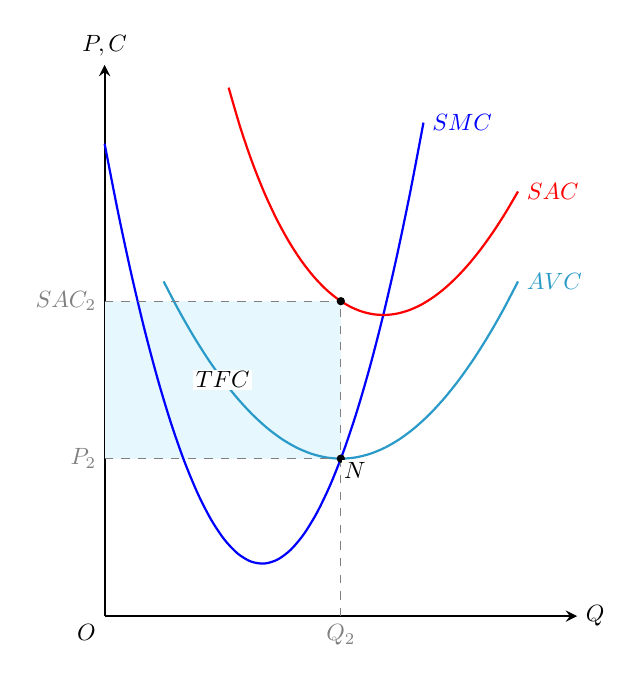
\begin{tikzpicture}[x=1.5cm, y=1cm, >=stealth, thick, every node/.style={scale=0.85}]
				% 坐标轴
				\draw[->] (0,0) -- (4,0) node[right] {$Q$};
				\draw[->] (0,0) -- (0,7) node[above] {$P, C$};
				
				% 亏损面积填充 (防遮挡放底层)
				\fill[cyan!10] (0,2) rectangle (2,4);
				
				% 精确代数绘图
				% TVC = x^3 - 4x^2 + 6x  =>  AVC = x^2 - 4x + 6, min at (2,2)
				% SMC = 3x^2 - 8x + 6, intersects AVC min at (2,2)
				% TC = x^3 - 4x^2 + 6x + 4  =>  SAC = x^2 - 4x + 6 + 4/x
				% 严格限制 domain，防止函数值 Y 溢出坐标轴 (限制最高 y < 7)
				\draw[domain=0:2.7, smooth, variable=\x, blue] plot ({\x}, {3*\x*\x - 8*\x + 6}) node[right] {$SMC$};
				\draw[domain=0.5:3.5, smooth, variable=\x, cyan!80!black] plot ({\x}, {\x*\x - 4*\x + 6}) node[right] {$AVC$};
				\draw[domain=1.05:3.5, smooth, variable=\x, red] plot ({\x}, {\x*\x - 4*\x + 6 + 4/\x}) node[right] {$SAC$};
				
				% 辅助线与坐标点
				\draw[dashed, thin, gray] (2,0) node[below] {$Q_2$} -- (2,4);
				\draw[dashed, thin, gray] (0,4) node[left] {$SAC_2$} -- (2,4);
				\draw[dashed, thin, gray] (0,2) node[left] {$P_2$} -- (2,2);
				
				\fill (2,2) circle (1.5pt) node[below right, fill=white, inner sep=1pt] {$N$};
				\fill (2,4) circle (1.5pt);
				
				\node at (1,3) [fill=white, inner sep=1pt] {$TFC$};
				\node[below left] at (0,0) {$O$};
			\end{tikzpicture}
		\end{center}
		\newpage
		
		\item \textbf{解释为什么行业长期供给曲线不是行业长期边际成本曲线。}
		
		\textbf{答：}
		行业长期供给曲线并非行业内各厂商长期边际成本曲线（$LMC$）的简单水平加总。在完全竞争市场中，个别厂商的短期供给曲线确实是其短期边际成本曲线（$SMC$）高于平均可变成本（$AVC$）最低点的部分。这是因为在短期内，生产要素价格和行业规模被假定为不变。然而在长期内，随着市场需求的变动，厂商的自由进出不仅会改变行业总产量，更会引发核心生产要素价格的变动，从而导致厂商的整套成本曲线发生根本性的物理平移。
		
		为了清晰说明这一动态机制，我们可以结合如下的联动图示（以典型的成本递增行业为例）进行推导验证：
		
		第一阶段（初始长期均衡）： 如图 (b) 所示，初始市场需求为 $D_1$，行业总供给为 $S_1$，市场在 $E_1$ 点出清，决定了初始价格 $P_1$。对应到图 (a)，代表性厂商作为价格接受者，在 $P_1$ 的引导下，于长期平均成本曲线 $LAC_1$ 的最低点 $A$ 进行生产。此时经济利润为零，处于长期均衡状态。
		
		第二阶段（短期需求冲击）： 当市场需求增加导致需求曲线右移至 $D_2$ 时，短期内由于行业内厂商数量固定，价格飙升至 $P_2$（图 (b) 中的 $E_2$ 点）。面对高企的价格，图 (a) 中的厂商会沿着原有的边际成本曲线 $SMC_1$ 增加产量至点 $B$。此时 $P_2 > LAC_1$，厂商获得了丰厚的正经济利润。
		
		第三阶段（长期产能调整与成本平移）： 巨额的超额利润必然吸引大量新厂商跨越零壁垒涌入该行业。由于该行业是成本递增行业，全行业规模的急剧扩张导致对稀缺生产要素（如熟练技术工人、特定原材料）的争夺加剧，直接推高了要素采购价格。这一“外部不经济”现象导致单个厂商的成本曲线整体向上平移，从 $LAC_1$ 和 $SMC_1$ 漂移至 $LAC_2$ 和 $SMC_2$。
		
		第四阶段（新长期均衡与曲线生成）：与此同时，新厂商的涌入使得图 (b) 中的短期供给曲线右移至 $S_2$。随着供给的增加，市场价格从 $P_2$ 逐渐回落。当价格下降与不断攀升的 $LAC_2$ 在 $P_3$ 处相遇时（图 (b) 的 $E_3$ 点与图 (a) 的 $C$ 点），经济利润被彻底抹平，市场重新恢复长期零利润均衡状态。
		
		综上所述，连结图 (b) 中初始均衡点 $E_1$ 和新均衡点 $E_3$ 所得到的长期供给曲线 $LS$，反映的是在要素价格变动和厂商自由进出双重作用下，一系列不同 $LAC$ 最低点所对应的价格与总产量的连线轨迹。它是在无数条发生位移的成本曲线间穿梭的均衡点集合，而绝非单条静态的、假设要素价格不变的 $LMC$ 曲线的简单加总。
		
		\begin{center}
			\begin{tikzpicture}[x=0.8cm, y=0.8cm, >=stealth, thick, every node/.style={scale=0.85}]
				
				% ================= 贯穿左右两图的全局价格参考线 (置于底层防遮挡) =================
				\draw[dashed, thin, gray] (0,2) node[left, black] {$P_1$} -- (8.5,2);  % P=2 延伸至 E1
				\draw[dashed, thin, gray] (0,4) node[left, black] {$P_2$} -- (10.5,4); % P=4 延伸至 E2
				\draw[dashed, thin, gray] (0,3) node[left, black] {$P_3$} -- (11.5,3); % P=3 延伸至 E3
				
				% ================= 左图：代表性厂商 =================
				\draw[->] (0,0) -- (4.5,0) node[right] {$q$};
				\draw[->] (0,0) -- (0,5.5) node[above] {$P, C$};
				\node[below] at (2,-0.5) {(a) 代表性厂商};
				
				% 初始状态 1
				\draw[domain=0.6:3.4, smooth, variable=\x, blue] plot ({\x}, {0.8*(\x-2)*(\x-2) + 2}) node[right] {$LAC_1$};
				\draw[domain=1.2:3.3, smooth, variable=\x, blue] plot ({\x}, {1.8*(\x-2) + 2}) node[right] {$SMC_1$};
				
				% 扩张后状态 2 
				% 将 LAC2 的标签强行锚定在左侧定义域起点 x=0.2 处 (y=4.35)
				\draw[domain=0.2:2.8, smooth, variable=\x, red] plot ({\x}, {0.8*(\x-1.5)*(\x-1.5) + 3});
				\node[right,red] at (0.2, 4.35) {$LAC_2$};
				\draw[domain=0.6:2.7, smooth, variable=\x, red] plot ({\x}, {1.8*(\x-1.5) + 3}) node[left] {$SMC_2$};
				
				% 核心交点 (加入 fill=white 防遮挡)
				\fill (2,2) circle (1.5pt) node[below right, fill=white, inner sep=1pt] {$A$};
				\fill (1.5,3) circle (1.5pt) node[below left, fill=white, inner sep=1pt] {$C$};
				\fill (3.11,4) circle (1.5pt) node[right, fill=white, inner sep=1pt] {$B$};
				
				% 底部投影线
				\draw[dashed, thin, gray] (2,0) node[below, black] {$q_1$} -- (2,2);
				\draw[dashed, thin, gray] (1.5,0) node[below, black] {$q_3$} -- (1.5,3);
				\draw[dashed, thin, gray] (3.11,0) node[below, black] {$q_2$} -- (3.11,4);
				
				
				% ================= 右图：行业市场 =================
				\begin{scope}[xshift=6.5cm]
					\draw[->] (0,0) -- (6.5,0) node[right] {$Q$};
					\draw[->] (0,0) -- (0,5.5) node[above] {$P$};
					\node[below] at (3,-0.5) {(b) 竞争性行业};
					
					% 需求曲线
					\draw[domain=0.5:3.5, smooth, variable=\x, blue] plot ({\x}, {4-\x}) node[right] {$D_1$};
					\draw[domain=3:5.5, smooth, variable=\x, blue] plot ({\x}, {8-\x}) node[right] {$D_2$};
					
					% 短期供给曲线
					\draw[domain=0.5:4.5, smooth, variable=\x, cyan!80!black] plot ({\x}, {\x}) node[above] {$S_1$};
					\draw[domain=2.8:5.5, smooth, variable=\x, cyan!80!black] plot ({\x}, {\x-2}) node[right] {$S_2$};
					
					% 长期供给曲线 LS (稍微延长至 6.2 以错开 S2 标签)
					\draw[domain=1:6.2, smooth, variable=\x, orange, line width=1.2pt] plot ({\x}, {0.333*\x + 1.333}) node[right] {$LS$};
					
					% 交点 (全方位错开排版，加入 fill=white 清除交叉线干扰)
					\fill (2,2) circle (1.5pt) node[below=2pt, fill=white, inner sep=1.5pt] {$E_1$};
					\fill (4,4) circle (1.5pt) node[above=2pt, fill=white, inner sep=1.5pt] {$E_2$};
					\fill (5,3) circle (1.5pt) node[below right=2pt, fill=white, inner sep=1.5pt] {$E_3$};
					
					% 底部投影线
					\draw[dashed, thin, gray] (2,0) node[below, black] {$Q_1$} -- (2,2);
					\draw[dashed, thin, gray] (4,0) node[below, black] {$Q_2$} -- (4,4);
					\draw[dashed, thin, gray] (5,0) node[below, black] {$Q_3$} -- (5,3);
				\end{scope}
				
			\end{tikzpicture}
		\end{center}
		
		\newpage
		\item \textbf{在长期均衡时，行业中所有厂商的经济利润为零。为什么？}
		
		\textbf{答：}
		在完全竞争市场中，长期经济利润必然趋于零，其根本原因在于行业毫无壁垒的“自由进出”机制。
		
		若短期内行业存在正的经济利润，必然吸引新厂商进入。供给的增加会导致行业供给曲线右移、市场价格下降，从而持续挤压利润空间；反之，若价格过低导致经济亏损，部分厂商将退出市场，供给减少又会促使价格回升。这一动态博弈最终必然收敛于一点——价格恰好等于长期平均成本的最低点，所有厂商的经济利润被彻底抹平，进出市场的激励随之消失。
		
		需要指出的是，部分厂商由于拥有稀缺资源（如绝佳地段或顶尖管理才能），其账面上的“会计利润”可能远高于同行。但若扣除这些资源在别处能获得的最高报酬（即隐性机会成本或经济租金），其真实的经济利润依然为零。
		
		如下图所示，在长期均衡点 $E$ 处，厂商达成 $P = LMC = LAC = SMC = SAC$ 的四线共点完美状态，总收益严格等于总成本。
		
		\begin{center}
			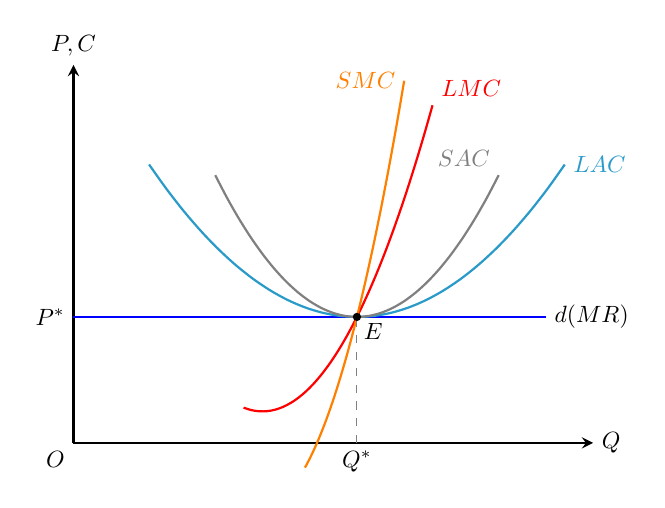
\begin{tikzpicture}[x=1.2cm, y=0.8cm, >=stealth, thick, every node/.style={scale=0.85}]
				% 坐标轴 (Y轴最高设定为6)
				\draw[->] (0,0) -- (5.5,0) node[right] {$Q$};
				\draw[->] (0,0) -- (0,6) node[above] {$P, C$};
				
				% 需求曲线与价格线
				\draw[blue, thick] (0,2) node[left, black] {$P^*$} -- (5,2) node[right, black] {$d (MR)$};
				
				% LAC = 0.5(x-3)^2 + 2, 最低点 (3,2)
				\draw[domain=0.8:5.2, smooth, variable=\x, cyan!80!black] plot ({\x}, {0.5*(\x-3)*(\x-3) + 2}) node[right] {$LAC$};
				
				% SAC = (x-3)^2 + 2, 最低点 (3,2)
				\draw[domain=1.5:4.5, smooth, variable=\x, gray] plot ({\x}, {(\x-3)*(\x-3) + 2}) node[above left] {$SAC$};
				
				% LMC = 1.5x^2 - 6x + 6.5. 严格限制 domain 防止 Y>6
				\draw[domain=1.8:3.8, smooth, variable=\x, red] plot ({\x}, {1.5*\x*\x - 6*\x + 6.5}) node[above right] {$LMC$};
				
				% SMC = 3x^2 - 12x + 11. 严格限制 domain 防止 Y>6
				\draw[domain=2.45:3.5, smooth, variable=\x, orange] plot ({\x}, {3*\x*\x - 12*\x + 11}) node[left] {$SMC$};
				
				% 均衡点与辅助线
				\draw[dashed, thin, gray] (3,0) node[below, black] {$Q^*$} -- (3,2);
				\fill (3,2) circle (1.5pt) node[below right=1pt, fill=white, inner sep=1.5pt] {$E$};
				
				\node[below left] at (0,0) {$O$};
			\end{tikzpicture}
		\end{center}
		
		\item \textbf{经济利润和生产者剩余之间有什么不同？}
		
		\textbf{答：}
		经济利润与生产者剩余之间的核心差额即为生产的总固定成本（$TFC$）。经济利润是指属于企业所有者的、超过生产过程中所运用的所有要素的机会成本的一种收益，在数值上它等于总收益（$TR$）与总成本（$TC$）的差额。而生产者剩余则是指厂商在提供一定数量的产品时，实际接受的总支付与愿意接受的最小总支付之间的差额。
		
		在几何图形上，生产者剩余通常用市场价格线以下、短期边际成本（$SMC$）曲线以上的面积来表示。这是因为在短期内固定成本无法改变，边际成本的积分即为总可变成本（$TVC$）。只要价格大于边际成本，厂商每多生产一单位产品就能获得额外的剩余价值。两者的代数关系可严格表述为：
		\[
		\begin{aligned}
			\text{经济利润} (\pi) &= TR - TC = TR - (TVC + TFC) \\
			\text{生产者剩余} (PS) &= TR - TVC \\
			\implies PS - \pi &= TFC
		\end{aligned}
		\]
		总之，即使短期内经济利润为负，只要生产者剩余为正且能弥补部分固定成本，厂商依然有动力维持生产。
		
		\begin{center}
			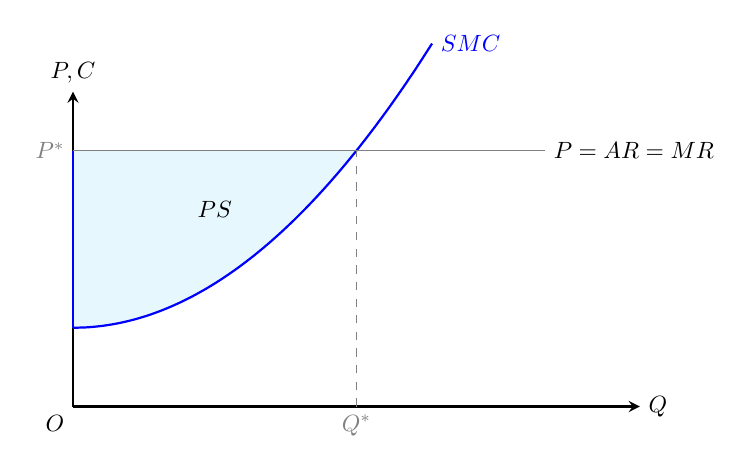
\begin{tikzpicture}[x=1.2cm, y=0.5cm, >=stealth, thick, every node/.style={scale=0.85}]
				% 坐标轴
				\draw[->] (0,0) -- (6,0) node[right] {$Q$};
				\draw[->] (0,0) -- (0,8) node[above] {$P, C$};
				
				% SMC = 0.5 * x^2 + 2, P* = 6.5
				% 交点 x = 3
				\fill[cyan!10] (0,6.5) -- (3,6.5) -- plot[domain=3:0, smooth, variable=\x] ({\x}, {0.5*\x*\x + 2}) -- (0,2) -- cycle;
				
				% 曲线与价格线
				\draw[domain=0:3.8, smooth, variable=\x, blue] plot ({\x}, {0.5*\x*\x + 2}) node[right] {$SMC$};
				\draw[blue] (0,2) -- (0,6.5); % 纵轴截距段
				\draw[thin, gray] (0,6.5) node[left] {$P^*$} -- (5,6.5) node[right, black] {$P=AR=MR$};
				
				% 辅助线
				\draw[dashed, thin, gray] (3,0) node[below] {$Q^*$} -- (3,6.5);
				
				\node at (1.5, 5) {$PS$};
				\node[below left] at (0,0) {$O$};
			\end{tikzpicture}
		\end{center}
		
		\item \textbf{当厂商知道在长期它们的经济利润为零时，它们为什么还进入这个行业？}
		
		\textbf{答：}
		厂商在明知长期经济利润为零的前提下依然选择进入行业，主要基于短期套利动机与机会成本补偿两方面的考量。
		
		首先，长期均衡的实现是一个漫长的动态调整过程。在向零利润状态收敛的短期和中期内，受市场需求激增或技术创新影响，行业内往往存在可观的正经济利润。由于进入竞争性行业的门槛极低，厂商完全可以为了捕获这些短期的超额利润而果断入场。
		
		其次，零经济利润绝不意味着厂商陷入账面亏损，而是表明厂商的所有生产要素（包括企业家的资本和时间）都获得了正常利润。换言之，厂商投资该行业的收益率已经完全覆盖了其最佳替代选择的机会成本。此时厂商的资源配置已达到有效状态，自然没有任何动机退出该行业。
		
		\item \textbf{在 20 世纪初，美国有许多小的汽车生产厂家，20 世纪末仅有三家大的厂家。假设这种情况不是反垄断法实施不力的结果，你怎样解释汽车制造厂家的数量减少？（提示：汽车行业的固有成本结构是怎样的？）}
		
		\textbf{答：}
		汽车制造厂家数量的剧减，深刻反映了该行业资本密集型属性所内生的规模经济效应。
		
		汽车产业的固有成本结构呈现出极高的固定成本（如庞大的冲压设备、流水线与研发投入）和相对较低的边际成本特征。这意味着在极大的产量范围内，企业的长期平均成本（$LAC$）会随着产量的增加而持续大幅下降。在长期演进中，率先扩大生产规模的厂商能够有效摊薄巨额固定成本，从而以远低于竞争对手的单位成本和价格向市场提供产品。
		
		面对大型厂商主导的不断探底的市场价格，未能实现规模扩张的小型厂商将面临长期亏损的境地，最终被迫退出市场。随着市场份额向少数几家巨头集中，行业逐渐形成了寡头垄断甚至准自然垄断的格局。因此，厂家数量的减少并非单纯的市场失灵，而是市场追求成本最小化和规模报酬递增的自然演化结果。
		
		\newpage
		\item \textbf{因为 X 行业是完全竞争的，该行业的每个厂商的经济利润为零。如果产品价格下降，没有厂商可以生存。你同意还是不同意这种认识？讨论一下。}
		
		\textbf{答：}
		不同意此观点。这种认识严重混淆了微观经济学中的短期经营决策准则与长期市场动态调整机制。
		
		在短期内，如果市场需求收缩导致产品价格下降，只要新价格并未跌破厂商平均可变成本（$AVC$）的最低点，即满足 $P > AVC_{\min}$ 的停业原则，厂商为了最大程度地弥补固定成本带来的沉没亏损，依然会理性选择继续维持生产。由于全行业各厂商的短期成本结构必然存在异质性，只要价格不跌破所有厂商的 $AVC$ 最低点，短期内就绝不会出现全行业覆灭的现象。
		
		在长期内，持续的经济亏损确实会导致部分处于劣势的厂商退出市场。然而，根据竞争市场的自发调节机制，大量厂商的退出会导致行业总供给骤减，促使短期行业供给曲线向左上方移动。这一动态收缩过程会持续推高市场均衡价格。当价格回升至代表性厂商长期平均成本（$LAC$）的最低点时，退出过程停止，市场达到新的长期均衡。此时，留在行业内的幸存厂商其经济利润恢复为零，能够继续稳定生存。
		
		如下方联动图所示，市场价格在短期内受需求冲击从 $P_1$ 跌至 $P_2$，但由于 $P_2$ 依然高于 $AVC$ 的最低点 $N$，厂商在短期内存活；长期内供给收缩（$S_1 \to S_2$），价格重新回归 $P_1$。
		
		\begin{center}
			\begin{tikzpicture}[x=1cm, y=0.8cm, >=stealth, thick, every node/.style={scale=0.85}]
				
				% ================= 左图：代表性厂商 =================
				\draw[->] (0,0) -- (4.5,0) node[right] {$q$};
				\draw[->] (0,0) -- (0,7) node[above] {$P, C$};
				\node[below] at (2,-0.5) {(a) 代表性厂商};
				
				% 代数基准：TC = x^3 - 4x^2 + 5.5x + 6.25
				% AVC = x^2 - 4x + 5.5, min at N(2, 1.5)
				% SMC = 3x^2 - 8x + 5.5, passes (2, 1.5) and (2.5, 4.25)
				% SAC = x^2 - 4x + 5.5 + 6.25/x, min at A(2.5, 4.25)
				\draw[domain=0.5:3.5, smooth, variable=\x, cyan!80!black] plot ({\x}, {\x*\x - 4*\x + 5.5}) node[right] {$AVC$};
				\draw[domain=1.2:3.5, smooth, variable=\x, red] plot ({\x}, {\x*\x - 4*\x + 5.5 + 6.25/\x}) node[right] {$SAC(LAC)$};
				\draw[domain=1.3:2.8, smooth, variable=\x, blue] plot ({\x}, {3*\x*\x - 8*\x + 5.5}) node[right] {$SMC$};
				
				\fill (2.5, 4.25) circle (1.5pt) node[above left, fill=white, inner sep=1pt] {$A$};
				\fill (2, 1.5) circle (1.5pt) node[below right, fill=white, inner sep=1pt] {$N(AVC_{\min})$};
				
				% ================= 右图：行业市场 =================
				\begin{scope}[xshift=6cm]
					\draw[->] (0,0) -- (5.5,0) node[right] {$Q$};
					\draw[->] (0,0) -- (0,7) node[above] {$P$};
					\node[below] at (2.5,-0.5) {(b) 竞争性行业};
					
					% D1: P = -Q + 8.25. D2: P = -Q + 5.5
					\draw[domain=1.5:5, smooth, variable=\x, blue] plot ({\x}, {-\x + 8.25}) node[right] {$D_1$};
					\draw[domain=0.5:4.5, smooth, variable=\x, blue] plot ({\x}, {-\x + 5.5}) node[right] {$D_2$};
					
					% S1: P = Q + 0.25. S2: P = Q + 3
					\draw[domain=1.5:5.5, smooth, variable=\x, cyan!80!black] plot ({\x}, {\x + 0.25}) node[right] {$S_1$};
					\draw[domain=0.2:3.5, smooth, variable=\x, cyan!80!black] plot ({\x}, {\x + 3}) node[above] {$S_2$};
					
					% 交点
					\fill (4, 4.25) circle (1.5pt) node[above=2pt, fill=white, inner sep=1.5pt] {$E_1$};
					\fill (2.625, 2.875) circle (1.5pt) node[below=2pt, fill=white, inner sep=1.5pt] {$E_2$};
					\fill (1.25, 4.25) circle (1.5pt) node[above left=2pt, fill=white, inner sep=1.5pt] {$E_3$};
					
					% 投影
					\draw[dashed, thin, gray] (4,0) node[below, black] {$Q_1$} -- (4,4.25);
					\draw[dashed, thin, gray] (2.625,0) node[below, black] {$Q_2$} -- (2.625,2.875);
					\draw[dashed, thin, gray] (1.25,0) node[below, black] {$Q_3$} -- (1.25,4.25);
				\end{scope}
				
				% ================= 贯穿左右全局投影 =================
				% P1 = 4.25
				\draw[dashed, thin, gray] (0,4.25) node[left, black] {$P_1$} -- (10,4.25);
				% P2 = 2.875
				\draw[dashed, thin, gray] (0,2.875) node[left, black] {$P_2$} -- (8.625,2.875);
				
			\end{tikzpicture}
		\end{center}
		
		\item \textbf{对音像电影的需求增加也可以增加演员的薪水。解释电影的长期供给曲线是水平的还是向上倾斜的。}
		
		\textbf{答：}
		电影行业的长期供给曲线是向上倾斜的。这一现象深刻反映了该行业属于微观经济学中典型的“成本递增行业”。
		
		长期供给曲线的最终形状，取决于全行业规模扩张对核心生产要素价格的冲击程度。随着市场对音像电影需求的急剧增加，行业内的制作公司纷纷扩大生产规模，导致对特定生产要素（特别是高水平的主演演员）的需求量激增。由于顶尖演员的供给在长期内依然具有极强的稀缺性（缺乏弹性），这种强烈的要素需求不可避免地拉动了演员薪水在全行业的系统性上涨。
		
		要素采购价格的攀升，意味着企业的生产具有“外部不经济”特征，这将直接导致所有电影制作厂商的平均成本曲线与边际成本曲线发生整体向上的物理平移。因此，整个电影行业必须在更高的市场价格水平下，才能重新覆盖上涨的成本并实现长期零利润均衡。连结新旧均衡点所描绘出的轨迹，便是一条向右上方倾斜的长期供给曲线（$LS$）。
		
		\begin{center}
			\begin{tikzpicture}[x=0.8cm, y=0.8cm, >=stealth, thick, every node/.style={scale=0.85}]
				
				% 全局价格参考线 (置于底层防遮挡)
				\draw[dashed, thin, gray] (0,2) node[left, black] {$P_1$} -- (8.5,2); 
				\draw[dashed, thin, gray] (0,4) node[left, black] {$P_2$} -- (10.5,4);
				\draw[dashed, thin, gray] (0,3) node[left, black] {$P_3$} -- (11.5,3);
				
				% ================= 左图：代表性厂商 =================
				\draw[->] (0,0) -- (4.5,0) node[right] {$q$};
				\draw[->] (0,0) -- (0,5.5) node[above] {$P, C$};
				\node[below] at (2,-0.5) {(a) 电影制作厂商};
				
				% 初始成本状态
				\draw[domain=0.6:3.4, smooth, variable=\x, blue] plot ({\x}, {0.8*(\x-2)*(\x-2) + 2}) node[right] {$LAC_1$};
				\draw[domain=1.2:3.3, smooth, variable=\x, blue] plot ({\x}, {1.8*(\x-2) + 2}) node[right] {$SMC_1$};
				
				% 演员薪水上涨导致成本平移
				\draw[domain=0.2:2.8, smooth, variable=\x, red] plot ({\x}, {0.8*(\x-1.5)*(\x-1.5) + 3});
				\node[right,red] at (0.2, 4.35) {$LAC_2$};
				\draw[domain=0.6:2.7, smooth, variable=\x, red] plot ({\x}, {1.8*(\x-1.5) + 3}) node[left] {$SMC_2$};
				
				\fill (2,2) circle (1.5pt) node[below right, fill=white, inner sep=1pt] {$A$};
				\fill (1.5,3) circle (1.5pt) node[below left, fill=white, inner sep=1pt] {$C$};
				
				\draw[dashed, thin, gray] (2,0) node[below, black] {$q_1$} -- (2,2);
				\draw[dashed, thin, gray] (1.5,0) node[below, black] {$q_3$} -- (1.5,3);
				
				% ================= 右图：行业市场 =================
				\begin{scope}[xshift=6.5cm]
					\draw[->] (0,0) -- (6.5,0) node[right] {$Q$};
					\draw[->] (0,0) -- (0,5.5) node[above] {$P$};
					\node[below] at (3,-0.5) {(b) 电影产业市场};
					
					% 需求增加
					\draw[domain=0.5:3.5, smooth, variable=\x, blue] plot ({\x}, {4-\x}) node[right] {$D_1$};
					\draw[domain=3:5.5, smooth, variable=\x, blue] plot ({\x}, {8-\x}) node[right] {$D_2$};
					
					% 供给扩张
					\draw[domain=0.5:4.5, smooth, variable=\x, cyan!80!black] plot ({\x}, {\x}) node[above] {$S_1$};
					\draw[domain=2.8:5.5, smooth, variable=\x, cyan!80!black] plot ({\x}, {\x-2}) node[right] {$S_2$};
					
					% 向上倾斜的长期供给曲线
					\draw[domain=1:6.2, smooth, variable=\x, orange, line width=1.2pt] plot ({\x}, {0.333*\x + 1.333}) node[right] {$LS$};
					
					\fill (2,2) circle (1.5pt) node[below=2pt, fill=white, inner sep=1.5pt] {$E_1$};
					\fill (4,4) circle (1.5pt) node[above=2pt, fill=white, inner sep=1.5pt] {$E_2$};
					\fill (5,3) circle (1.5pt) node[below right=2pt, fill=white, inner sep=1.5pt] {$E_3$};
					
					\draw[dashed, thin, gray] (2,0) node[below, black] {$Q_1$} -- (2,2);
					\draw[dashed, thin, gray] (4,0) node[below, black] {$Q_2$} -- (4,4);
					\draw[dashed, thin, gray] (5,0) node[below, black] {$Q_3$} -- (5,3);
				\end{scope}
				
			\end{tikzpicture}
		\end{center}
		
		\item \textbf{判断正误：一个厂商的生产总是在长期平均成本最小化的地方。解释一下。}
		
		\textbf{答：}
		错误。该观点忽略了短期与长期决策条件的区别，以及不同市场结构下的效率差异。
		
		在短期内，由于存在无法自由调整的固定生产要素，厂商只能遵循边际收益等于短期边际成本（$MR = SMC$）的原则进行生产。受限于既定的工厂规模，此时的短期均衡产量完全可能偏离长期平均成本（$LAC$）的最低点。
		
		即便在长期（所有生产要素均可调整），也只有在完全竞争市场的长期动态均衡状态下，自由进出机制才会迫使厂商在 $LAC$ 的最低点进行生产（满足 $P = MR = LMC = LAC_{\min}$）。而在诸如垄断或垄断竞争等市场结构中，厂商面临向下倾斜的需求曲线，其长期均衡点往往落在 $LAC$ 曲线向下或向上倾斜的阶段，而非最低点。
		
		如下图所示，若市场需求使得厂商在短期选择在 $Q_1$ 处生产最优，厂商会构建一个对应于 $SAC$ 的短期生产规模，使 $SAC$ 与 $LAC$ 在点 $A$ 精确相切。显然，生产切点 $A$ 并非长期平均成本的最低点 $B$（对应规模 $Q_2$）。
		
		\begin{center}
			\begin{tikzpicture}[x=1.2cm, y=0.6cm, >=stealth, thick, every node/.style={scale=0.85}]
				% 坐标轴
				\draw[->] (0,0) -- (6.5,0) node[right] {$Q$};
				\draw[->] (0,0) -- (0,8.5) node[above] {$C$};
				
				% 核心代数函数驱动，确保数学绝对相切
				% LAC = 0.5(x-4)^2 + 4, min at B(4,4)
				\draw[domain=1.5:6.2, smooth, variable=\x, blue] plot ({\x}, {0.5*(\x-4)*(\x-4) + 4}) node[right] {$LAC$};
				
				% SAC = 1.5x^2 - 8x + 16
				% At x=2: SAC(2) = 6, SAC'(2) = -2. LAC(2) = 6, LAC'(2) = -2. 完美相切于 A(2,6).
				\draw[domain=1.2:3.5, smooth, variable=\x, red] plot ({\x}, {1.5*\x*\x - 8*\x + 16}) node[right] {$SAC$};
				
				% 切点与极值点
				\fill (2,6) circle (1.5pt) node[above right] {$A$};
				\fill (4,4) circle (1.5pt) node[below right] {$B$};
				
				% 辅助线
				\draw[dashed, thin, gray] (2,0) node[below, black] {$Q_1$} -- (2,6);
				\draw[dashed, thin, gray] (4,0) node[below, black] {$Q_2$} -- (4,4);
				
				\node[below left] at (0,0) {$O$};
			\end{tikzpicture}
		\end{center}
		
		\item \textbf{在具有向上倾斜的供给曲线的行业，能存在规模报酬不变吗？}
		
		\textbf{答：}
		完全能够存在。这种认知必须严格区分生产函数的“技术属性”与行业层面的“外部经济/不经济属性”。
		
		规模报酬不变是单个厂商生产函数的内在纯技术特征。它意味着当单个厂商在物理层面上将所有投入要素同比例增加时，其实际产量也会以完全相同的比例增加（即 $F(tK, tL) = tF(K, L)$）。
		
		相反，行业拥有向上倾斜的长期供给曲线，是因为该行业呈现成本递增特征，这属于市场价格范畴。当行业内的所有企业为了满足市场需求而集体同时扩张时，会打破原有要素市场的供求平衡，推高稀缺生产要素（如特殊土地、专业技术劳力）的市场采购价格。因此，即便厂商在物理技术上实现了投入与产出的双倍增加（规模报酬不变），但由于要素单价的上涨，其总成本的上升幅度将远超两倍。总而言之，由于外部要素价格变动导致的行业成本递增，与厂商内部的规模报酬不变，在微观逻辑上可以完美并存。
		
		\item \textbf{市场是完全竞争的必要假设有哪些？根据本章所学，解释为什么这些假设都是重要的。}
		
		\textbf{答：}
		完全竞争市场是一种理想化的基准市场结构，其赖以成立的必要假设主要包括以下三个核心维度，它们在微观经济分析中具有不可替代的作用：
		
		价格接受者。假设市场中存在无数极小规模的买者和卖者，任何单一主体的买卖行为都不足以对总体市场价格施加可见的影响。这一假设至关重要，它使得单个厂商面临的需求曲线退化为一条由市场供需决定的水平线。这确保了厂商的边际收益严格等于市场价格（$MR = P$），从而将一般的利润最大化条件 $MC = MR$ 转化为完全竞争特有的黄金准则 $MC = P$。
		
		产品同质性。假设所有生产者向市场提供的均是物理属性与消费者主观认知上完全无差异的同质产品。该假设排除了厂商通过品牌溢价、包装或质量差异进行非价格竞争的可能。它不仅是实现“一物一价”市场定律的前提，更保证了价格机制在资源引导中作为唯一信号的纯粹性。
		
		自由进出。假设厂商进入或退出该行业不存在任何显著的沉没成本、技术壁垒或政策限制。这一动态假设是微观经济学推导长期均衡的基础。它构筑了优胜劣汰的调节机制：超额利润将无阻碍地吸引新进入者摊薄利润，而亏损将导致资源退出。最终，它驱使所有厂商的长期经济利润收敛于零（即生产点落在 $P = LAC_{\min}$），从而保证整个竞争性市场的产出实现了帕累托最优配置。
		
		\item \textbf{假设一个竞争性行业面临着需求的增长（即曲线向上移动）。一个竞争市场保证产出增加的步骤是什么？如果政府限制了最高价，你的答案会不会改变？}
		
		\textbf{答：}
		当行业需求激增（需求曲线由 $D_1$ 右移至 $D_2$）时，产出的增加与长期均衡的恢复经历以下动态步骤：
		
		短期内，行业供给曲线 $S_1$ 保持不变，需求冲击使市场价格从 $P_1$ 飙升至 $P_2$（均衡点由 $E_1$ 移至 $E_2$）。高价诱使现有厂商沿短期边际成本曲线扩产，并获得超额经济利润。长期内，超额利润吸引新厂商无壁垒涌入。新产能的加入促使短期供给曲线右移至 $S_2$，不断压低市场价格。当价格回落至原始水平 $P_1$ 时（点 $E_3$），利润归零，市场达成新的长期均衡。连结 $E_1$ 与 $E_3$ 即得到水平的长期供给曲线 $LS$。
		
		若政府施加了有效最高限价 $P_{\max}$（处于 $P_1$ 与 $P_2$ 之间）：短期内价格被压制在 $P_{\max}$，厂商仅愿意提供 $Q_A$ 的产量，而市场需求高达 $Q_B$，产生严重的供需短缺。然而，只要限价 $P_{\max}$ 仍高于长期平均成本（即仍有利润），新厂商就会随时间推移持续进入（$S_1 \to S_2$）。当供给的增加最终消除短缺、价格压力解除时，市场依然会收敛于零利润状态。因此，限价不改变长期产出增加的总趋势，但会严重扭曲短期资源配置并极大地拉长调整周期。
		
		\begin{center}
			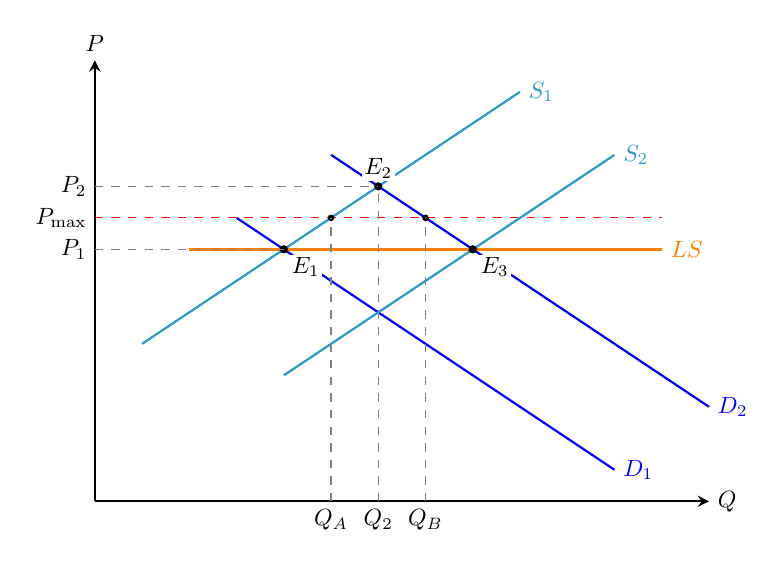
\begin{tikzpicture}[x=1.2cm, y=0.8cm, >=stealth, thick, every node/.style={scale=0.85}]
				% 坐标轴
				\draw[->] (0,0) -- (6.5,0) node[right] {$Q$};
				\draw[->] (0,0) -- (0,7) node[above] {$P$};
				
				% 需求曲线 D1, D2
				\draw[domain=1.5:5.5, smooth, variable=\x, blue] plot ({\x}, {6-\x}) node[right] {$D_1$};
				\draw[domain=2.5:6.5, smooth, variable=\x, blue] plot ({\x}, {8-\x}) node[right] {$D_2$};
				
				% 短期供给曲线 S1, S2
				\draw[domain=0.5:4.5, smooth, variable=\x, cyan!80!black] plot ({\x}, {\x+2}) node[right] {$S_1$};
				\draw[domain=2:5.5, smooth, variable=\x, cyan!80!black] plot ({\x}, {\x}) node[right] {$S_2$};
				
				% 长期供给曲线 LS
				\draw[domain=1:6, smooth, variable=\x, orange, line width=1.2pt] plot ({\x}, {4}) node[right] {$LS$};
				
				% 政府限价线 P_max
				\draw[dashed, thin, red] (0,4.5) node[left, black] {$P_{\max}$} -- (6,4.5);
				
				% 交点 (严格防重叠排版)
				\fill (2,4) circle (1.5pt) node[below right=2pt, fill=white, inner sep=1pt] {$E_1$};
				\fill (3,5) circle (1.5pt) node[above=2pt, fill=white, inner sep=1pt] {$E_2$};
				\fill (4,4) circle (1.5pt) node[below right=2pt, fill=white, inner sep=1pt] {$E_3$};
				
				% 限价导致的供需缺口端点
				\fill (2.5,4.5) circle (1.2pt);
				\fill (3.5,4.5) circle (1.2pt);
				
				% 投影线
				\draw[dashed, thin, gray] (2.5,0) node[below, black] {$Q_A$} -- (2.5,4.5);
				\draw[dashed, thin, gray] (3.5,0) node[below, black] {$Q_B$} -- (3.5,4.5);
				\draw[dashed, thin, gray] (3,0) node[below, black] {$Q_2$} -- (3,5);
				
				\draw[dashed, thin, gray] (0,5) node[left, black] {$P_2$} -- (3,5);
				\draw[dashed, thin, gray] (0,4) node[left, black] {$P_1$} -- (2,4);
			\end{tikzpicture}
		\end{center}
		
		\item \textbf{政府通过了一项法令，允许对每英亩用于种植烟草的土地给予补贴。这一措施会怎样影响烟草的长期供给曲线？}
		
		\textbf{答：}
		该补贴政策将导致烟草行业的长期供给曲线整体垂直向下（或向右下方）平移。
		
		政府按面积发放补贴，实质上外生地抵消了厂商的部分生产成本，导致整个行业的平均成本和边际成本曲线整体向下平移。如图所示，若市场初始均衡于点 $E_1$，成本下移会使现有农户瞬间获得超额利润。这一价格信号必然吸引新农户转产进入，并促使原有农户扩大种植。全行业供给激增导致市场价格持续下行。
		
		该扩张过程会一直持续到价格完全跌落至扣除补贴后的新平均成本最低点（即价格下降至 $P_2$），经济利润再次归零。宏观上，这必然表现为行业的长期供给曲线由 $LS_1$ 平移至 $LS_2$（平移量即为单位产量的补贴额度），最终市场在点 $E_2$ 达成新均衡，均衡价格永久性降低，总产出增加。
		
		\begin{center}
			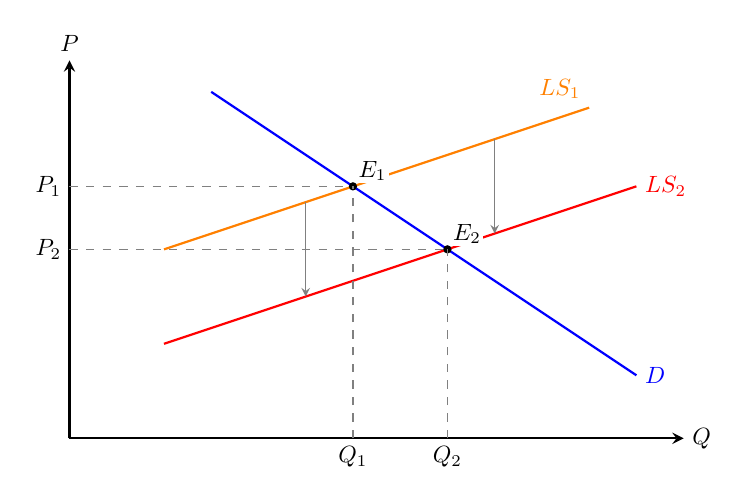
\begin{tikzpicture}[x=1.2cm, y=0.8cm, >=stealth, thick, every node/.style={scale=0.85}]
				% 坐标轴
				\draw[->] (0,0) -- (6.5,0) node[right] {$Q$};
				\draw[->] (0,0) -- (0,6) node[above] {$P$};
				
				% 需求曲线 D (P = 7 - Q)
				\draw[domain=1.5:6, smooth, variable=\x, blue] plot ({\x}, {7-\x}) node[right] {$D$};
				
				% 初始长期供给曲线 LS1 (P = 0.5Q + 2.5) 
				\draw[domain=1:5.5, smooth, variable=\x, orange] plot ({\x}, {0.5*\x + 2.5}) node[above left] {$LS_1$};
				
				% 补贴后的长期供给曲线 LS2 (P = 0.5Q + 1)，向下平移 1.5
				\draw[domain=1:6, smooth, variable=\x, red] plot ({\x}, {0.5*\x + 1}) node[right] {$LS_2$};
				
				% 核心交点 
				\fill (3,4) circle (1.5pt) node[above right=1pt, fill=white, inner sep=1pt] {$E_1$};
				\fill (4,3) circle (1.5pt) node[above right=1pt, fill=white, inner sep=1pt] {$E_2$};
				
				% 平移指示箭头
				\draw[->, thin, gray] (2.5, 3.75) -- (2.5, 2.25);
				\draw[->, thin, gray] (4.5, 4.75) -- (4.5, 3.25);
				
				% 投影线
				\draw[dashed, thin, gray] (3,0) node[below, black] {$Q_1$} -- (3,4);
				\draw[dashed, thin, gray] (4,0) node[below, black] {$Q_2$} -- (4,3);
				\draw[dashed, thin, gray] (0,4) node[left, black] {$P_1$} -- (3,4);
				\draw[dashed, thin, gray] (0,3) node[left, black] {$P_2$} -- (4,3);
			\end{tikzpicture}
		\end{center}
		\newpage
		\item \textbf{一个地区有若干家本地商店以及其他直销点或网站销售某种品牌的真空吸尘器。假如所有销售商要价相同，他们的长期经济利润是否都等于零？假如所有销售商要价相同，但是一家当地商店的经营场所为他自己拥有的房子，不必付租金，这个销售商的经济利润为正吗？不必付租金的这家销售商是否有激励去降低其销售价格？}
		
		\textbf{答：}
		如果所有销售商要价相同，他们的长期经济利润必然都等于零。在高度竞争的零售市场中，若存在超额利润，无壁垒的特性将迅速吸引新竞争者涌入，摊薄客流并压低毛利；若全行业亏损则会引发退出潮。市场的动态调整终将抹平所有超额收益。
		
		该免租商店的经济利润依然为零。免交租金仅使其账面上的“会计利润”虚高，但自有商业房产存在“机会成本”（即按市价出租给他人可获得的最高租金收益）。经济学的核心利润测算公式为：
		\[
		\begin{aligned}
			\text{经济利润} = \text{总收益} - (\text{显性会计成本} + \text{隐性机会成本})
		\end{aligned}
		\]
		该房屋作为商业门市的地段溢价，恰好被其自身高昂的隐性地租完全抵消。扣除这一机会成本后，其真实经济利润与其他需要按月付租金的竞品没有区别。
		
		该免租销售商毫无激励去主动降低销售价格。在完全竞争市场中，该商店面临一条近乎完全弹性的水平需求曲线。按照当前的市价，他完全有能力出清所有库存。盲目降价不仅无法让他长期垄断市场，反而会白白流失边际收益（$MR$），导致原本为零的经济利润直接跌成负值。因此，安于接受市价是其维持利润最大化的唯一理性决策。
		
	\end{enumerate}
	\newpage
	\section{练习题}
	\begin{enumerate}[label=\textbf{\arabic*.}, leftmargin=*]
		\item \textbf{下表给出了一家厂商的单位产品销售价格（单位：美元）和总成本的信息。假设你需要填充表中空格，并分析：如果价格从 60 美元下降到 50 美元，企业的产量选择和利润将发生何种变化？}
		
		\textbf{答：}
		首先，基于收益、成本与利润的基本核算逻辑可推导出表中的各项经营指标。其次，当市场价格为 60 美元时，企业遵循利润最大化原则（$MR=MC$），将最优产量设定为 10 个单位，获取最大利润 190 美元。最终，若价格滑落至 50 美元，边际收益同步下沉，企业必须将产量相应缩减至 9 个单位以重新实现均衡，此时最高利润亦随之缩水至 95 美元。
		
		\begin{center}
			\footnotesize
			\setlength{\tabcolsep}{2pt}
			\begin{tabularx}{\linewidth}{@{} *{10}{>{\centering\arraybackslash}X} @{}}
				\toprule
				& & \multicolumn{2}{c}{$R$} & $\pi$ & $MC$ & $MR$ & $R$ & $MR$ & $\pi$ \\
				\cmidrule(lr){3-4} \cmidrule(lr){5-5} \cmidrule(lr){6-7} \cmidrule(lr){8-10}
				$q$ & $P$ & $P=60$ & $C$ & $P=60$ & $P=60$ & $P=60$ & $P=50$ & $P=50$ & $P=50$ \\
				\midrule
				0 & 60 & 0 & 100 & -100 & — & — & 0 & — & -100 \\
				1 & 60 & 60 & 150 & -90 & 50 & 60 & 50 & 50 & -100 \\
				2 & 60 & 120 & 178 & -58 & 28 & 60 & 100 & 50 & -78 \\
				3 & 60 & 180 & 198 & -18 & 20 & 60 & 150 & 50 & -48 \\
				4 & 60 & 240 & 212 & 28 & 14 & 60 & 200 & 50 & -12 \\
				5 & 60 & 300 & 230 & 70 & 18 & 60 & 250 & 50 & 20 \\
				6 & 60 & 360 & 250 & 110 & 20 & 60 & 300 & 50 & 50 \\
				7 & 60 & 420 & 272 & 148 & 22 & 60 & 350 & 50 & 78 \\
				8 & 60 & 480 & 310 & 170 & 38 & 60 & 400 & 50 & 90 \\
				9 & 60 & 540 & 355 & 185 & 45 & 60 & 450 & 50 & 95 \\
				10 & 60 & 600 & 410 & 190 & 55 & 60 & 500 & 50 & 90 \\
				11 & 60 & 660 & 475 & 185 & 65 & 60 & 550 & 50 & 75 \\
				\bottomrule
			\end{tabularx}
		\end{center}
		
		\item \textbf{从上一题的数据进一步分析，如果固定成本从 100 美元增加到 150 美元，再增加到 200 美元，给定每单位 60 美元的价格保持不变，厂商的产出选择和利润会发生什么变化？从固定成本对厂商产出选择的影响中能得出什么一般结论？}
		
		\textbf{答：}
		首先，如表所示，随着固定成本从 100 美元递增至 200 美元，厂商在各产量上的总成本等额攀升，导致绝对利润被逐级压缩。其次，尽管利润总额缩水，厂商为实现利润最大化（或亏损最小化）的最优产量始终锚定在 10 个单位。最终可得出微观经济学的一般结论：在短期内，固定成本的高低对厂商的最优产出决策完全呈中性。因为利润最大化的一阶条件为边际收益等于边际成本（$MR = MC$），而固定成本作为常数，在对总成本求导时即被消除，不对边际成本构成任何影响，故最优产量维持不变。
		
		\begin{center}
			\footnotesize
			\setlength{\tabcolsep}{2pt}
			\begin{tabularx}{\linewidth}{@{} *{10}{>{\centering\arraybackslash}X} @{}}
				\toprule
				$q$ & $P$ & $TR$ & $TC_{FC=100}$ & $\pi_{FC=100}$ & $MC$ & $TC_{FC=150}$ & $\pi_{FC=150}$ & $TC_{FC=200}$ & $\pi_{FC=200}$ \\
				\midrule
				0 & 60 & 0 & 100 & -100 & — & 150 & -150 & 200 & -200 \\
				1 & 60 & 60 & 150 & -90 & 50 & 200 & -140 & 250 & -190 \\
				2 & 60 & 120 & 178 & -58 & 28 & 228 & -108 & 278 & -158 \\
				3 & 60 & 180 & 198 & -18 & 20 & 248 & -68 & 298 & -118 \\
				4 & 60 & 240 & 212 & 28 & 14 & 262 & -22 & 312 & -72 \\
				5 & 60 & 300 & 230 & 70 & 18 & 280 & 20 & 330 & -30 \\
				6 & 60 & 360 & 250 & 110 & 20 & 300 & 60 & 350 & 10 \\
				7 & 60 & 420 & 272 & 148 & 22 & 322 & 98 & 372 & 48 \\
				8 & 60 & 480 & 310 & 170 & 38 & 360 & 120 & 410 & 70 \\
				9 & 60 & 540 & 355 & 185 & 45 & 405 & 135 & 455 & 85 \\
				10 & 60 & 600 & 410 & 190 & 55 & 460 & 140 & 510 & 90 \\
				\bottomrule
			\end{tabularx}
		\end{center}
		\newpage
		\item \textbf{使用与上述相同的信息，请推导厂商的短期供给曲线。假如市场中存在 100 家相同的厂商，市场供给曲线将呈现何种形态？}
		
		\textbf{答：}
		首先，在完全竞争市场中，个体厂商的短期供给曲线是其平均可变成本（$AVC$）曲线最低点以上的边际成本（$MC$）曲线片段。如左图所示，当市场价格高于 $AVC$ 最低点（短期停业临界点）时，厂商将沿着向右上方倾斜的 $MC$ 曲线扩张产出。其次，行业的短期供给曲线是所有私人厂商供给曲线在水平方向上的加总。假设市场包含 100 家同质化厂商，则在任一给定价格下，市场总供给量均扩大为个体产量的 100 倍。如右图所示，加总后的市场短期供给曲线在纵向价格坐标上与个体保持一致，横轴规模则被等比例延展了 100 倍。
		
		\begin{center}
			\footnotesize
			\setlength{\tabcolsep}{2pt}
			\begin{tabularx}{0.8\linewidth}{@{} *{6}{>{\centering\arraybackslash}X} @{}}
				\toprule
				$q$ & $TC$ & $MC$ & $TVC$ & $TFC$ & $AVC$ \\
				\midrule
				0 & 100 & — & 0 & 100 & — \\
				1 & 150 & 50 & 50 & 100 & 50.0 \\
				2 & 178 & 28 & 78 & 100 & 39.0 \\
				3 & 198 & 20 & 98 & 100 & 32.7 \\
				4 & 212 & 14 & 112 & 100 & 28.0 \\
				5 & 230 & 18 & 130 & 100 & 26.0 \\
				6 & 250 & 20 & 150 & 100 & 25.0 \\
				7 & 272 & 22 & 172 & 100 & 24.6 \\
				8 & 310 & 38 & 210 & 100 & 26.3 \\
				9 & 355 & 45 & 255 & 100 & 28.3 \\
				10 & 410 & 55 & 310 & 100 & 31.0 \\
				11 & 475 & 65 & 375 & 100 & 34.1 \\
				\bottomrule
			\end{tabularx}
		\end{center}
		
		\begin{center}
			\begin{tikzpicture}[>=stealth, thick, every node/.style={scale=0.85}]
				% 全局辅助线 (底层防遮挡)
				\draw[dashed, gray, thin] (0, 1.47) -- (14, 1.47); % AVC min 对应的价格水位
				
				% 左图：个体厂商
				\begin{scope}[x=0.35cm, y=0.06cm]
					\draw[->] (0,0) -- (13,0) node[right] {$q$};
					\draw[->] (0,0) -- (0,75) node[above] {$C, P$};
					
					\draw[cyan!80!black] plot[smooth] coordinates {(1,50) (2,28) (3,20) (4,14) (5,18) (6,20) (7,22) (8,38) (9,45) (10,55) (11,65)} node[right] {$MC$};
					\draw[blue!70!black] plot[smooth] coordinates {(1,50) (2,39) (3,32.7) (4,28) (5,26) (6,25) (7,24.6) (8,26.3) (9,28.3) (10,31) (11,34.1)} node[right] {$AVC$};
					
					\node at (6, -10) {个体厂商};
				\end{scope}
				
				% 右图：市场供给
				\begin{scope}[xshift=7cm, x=0.0035cm, y=0.06cm]
					\draw[->] (0,0) -- (1300,0) node[right] {$Q$};
					\draw[->] (0,0) -- (0,75) node[above] {$P$};
					
					\draw[red!80!black] plot[smooth] coordinates {(700,24.6) (800,38) (900,45) (1000,55) (1100,65)} node[right] {$S$};
					
					\node at (600, -10) {市场供给};
				\end{scope}
			\end{tikzpicture}
		\end{center}
		
		\item \textbf{假设你是竞争市场上一家钟表制造厂的经理，你的生产成本函数为：$C = 200 + 2q^{2}$，其中 $q$ 为产出水平；$C$ 为总成本（该函数的边际成本为 $4q$，固定成本为 $200$ 美元）。如果市场价格定为 $100$ 美元，为追求利润最大化，你应该生产多少钟表并能获取多少利润？此外，厂商保持正产出的最低价格底线是多少？}
		
		\textbf{答：}
		首先，基于竞争性厂商面对既定市场价格的前提，钟表制造厂的总利润函数可被构建为总收益减去总成本的代数式。要实现利润极值，必须满足利润函数关于产量的一阶导数等于零的优化条件，即边际收益等于边际成本。通过构建一阶条件方程并代入 $P = 100$：
		\[
		\begin{aligned}
			\pi &= P q - C = 100 q - (200 + 2q^{2}) \\
			\frac{\mathrm{d}\pi}{\mathrm{d}q} &= 100 - 4q = 0
		\end{aligned}
		\]
		解得利润最大化的最优产出水平为 $q = 25$。其次，将最优产量反代回利润函数进行核算，可精确求得制造厂在该产量下的经济利润为：
		\[
		\begin{aligned}
			\pi &= 100 \times 25 - (200 + 2 \times 25^{2}) = 1050 \, \text{（美元）}
		\end{aligned}
		\]
		最终，关于企业的停业决策，微观经济学原理指出，在短期经营中只要总收益大于或等于总可变成本，厂商维持正产出便是有利的。这一底线条件等价于价格必须高于平均可变成本曲线的最低点。提取出平均可变成本函数与边际成本函数：
		\[
		\begin{aligned}
			AVC &= \frac{VC}{q} = \frac{2q^{2}}{q} = 2q \\
			MC &= 4q
		\end{aligned}
		\]
		从代数逻辑可知，对于任意正向产出 $q > 0$，恒存在 $MC > AVC$ 的不等式关系。这意味着平均可变成本曲线的最低端逼近原点。因此，只要市场价格微弱大于零，厂商在短期内就有充足的动力维持正的产出以弥补部分固定成本。
		
		\item \textbf{假设竞争性厂商生产产量为 $q$ 时的边际成本由下式给出：$MC(q) = 3 + 2q$。如果该产品的市场价格为 9 美元，厂商的产出水平与其对应的生产者剩余各是多少？若已知厂商的平均可变成本曲线为 $AVC(q) = 3 + q$，且固定成本为 3 美元，短期内厂商的利润状态是正、为负还是为零？}
		
		\textbf{答：}
		首先，身处完全竞争市场，厂商锁定最优产量的行为准则是将边际成本推至与市场价格齐平的边界。构建均衡等式 $P = MC$，即 $9 = 3 + 2q$，经过代数移项可迅速解得最优产出水平 $q = 3$。其次，衡量厂商在生产中获得的净福利，需计算生产者剩余。由于给定的边际成本函数呈现完美的线性特征，如图所示，生产者剩余在几何形态上严格映射为水平价格线与向右上倾斜的边际成本曲线之间所夹的阴影三角形面积。运用三角形面积公式计算如下：
		\[
		\begin{aligned}
			PS &= \frac{1}{2} \times (9 - 3) \times 3 = 9 \, \text{（美元）}
		\end{aligned}
		\]
		最终，为了探究底层的真实盈利状况，需要从可变成本与固定成本中还原出完整的总成本函数。根据题意推导总成本并将其引入利润等式中：
		\[
		\begin{aligned}
			TC(q) &= AVC(q) \times q + FC = (3 + q)q + 3 = 3q + q^{2} + 3 \\
			\pi &= TR - TC = 9q - (3q + q^{2} + 3)
		\end{aligned}
		\]
		将最优产量 $q = 3$ 代入上式进行最终核算，得出总利润 $\pi = 27 - (9 + 9 + 3) = 6$ 美元。由此可以做出严谨判定：在给定的市场与成本结构下，短期内厂商将斩获严格为正的经济利润。
		
		\begin{center}
			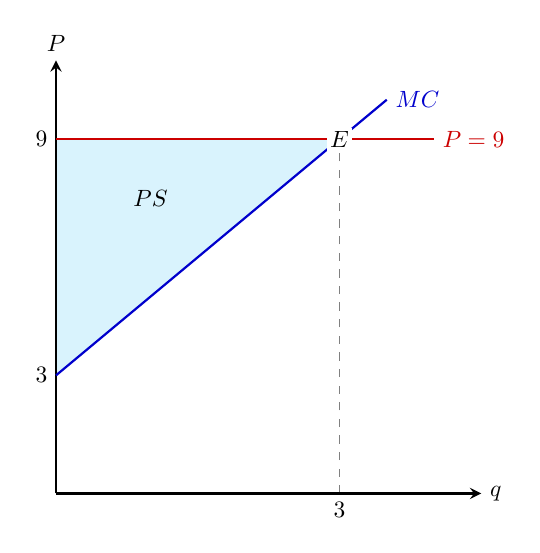
\begin{tikzpicture}[x=1.2cm, y=0.5cm, >=stealth, thick, every node/.style={scale=0.85}]
				% 1. 阴影面积填充 (置于底层)
				\fill[cyan!15] (0,3) -- (3,9) -- (0,9) -- cycle;
				
				% 2. 坐标轴与辅助线
				\draw[dashed, gray, thin] (3,0) -- (3,9);
				\draw[->] (0,0) -- (4.5,0) node[right] {$q$};
				\draw[->] (0,0) -- (0,11) node[above] {$P$};
				
				% 3. 核心曲线绘制
				\draw[blue!80!black, domain=0:3.5] plot (\x, {3 + 2*\x}) node[right] {$MC$};
				\draw[red!80!black] (0,9) -- (4,9) node[right] {$P=9$};
				
				% 4. 关键点与标签标注 (防遮挡)
				\node[fill=white, inner sep=1.5pt] at (3,9) {$E$};
				\node at (1, 7.5) {$PS$};
				\node[left] at (0,3) {$3$};
				\node[below] at (3,0) {$3$};
				\node[left] at (0,9) {$9$};
			\end{tikzpicture}
		\end{center}
		
		\item \textbf{竞争性市场中某厂商的生产成本函数为 $C = 50 + 4q + 2q^2$，边际成本函数为 $MC = 4 + 4q$。当市场价格给定为 20 美元时，若厂商产量为 5，厂商利润达到最大化了吗？在长期，厂商产量应该定为多少？}
		
		\textbf{答：}
		首先，在完全竞争市场下，厂商构筑利润最大化的绝对核心法则为边际收益等于边际成本（$P = MC$）。将给定的市场价格 $P=20$ 代入边际成本函数，构建一阶最优条件：
		\[
		\begin{aligned}
			20 &= 4 + 4q \\
			q &= 4
		\end{aligned}
		\]
		由此可知，当产量为 5 时，边际成本远超边际收益，厂商并未实现利润最大化，其最优产出水平应紧缩至 4 个单位。其次，基于该最优产量节点，核算厂商的当期绝对利润：
		\[
		\begin{aligned}
			\pi &= P q - C(q) \\
			&= 20 \times 4 - \left(50 + 4 \times 4 + 2 \times 4^{2}\right) \\
			&= 80 - 98 = -18
		\end{aligned}
		\]
		最终，利润核算表明，即便企业在边际上达到了最优（亏损最小化），其经济利润依然为负（$-18$）。基于微观经济学的长期动态调整机制，在价格与成本结构不发生根本性反转的前提下，长期内所有的固定成本将转化为可变成本，厂商无法承受持续的经济亏损，必将理性地选择退出该行业，此时的长期产量将归零。
		
		\item \textbf{假设厂商成本为 $C(q) = 16 + 4q^2$。请推导并绘制平均成本、固定成本、可变成本、平均可变成本和平均固定成本曲线。进一步求出使平均成本最小的产出水平，并界定在何种价格区间内厂商会保持正产量、承受负利润或赚取正利润。}
		
		\textbf{答：}
		首先，由总成本函数 $C(q) = 16 + 4q^2$ 可分离出固定成本 $FC = 16$ 与可变成本 $VC = 4q^2$。将其分别除以产量 $q$，可推导出平均可变成本 $AVC = 4q$，平均固定成本 $AFC = 16/q$，以及平均成本 $AC = 4q + 16/q$。其次，通过对总成本求导可得边际成本 $MC = 8q$。如图所示，平均成本曲线呈 U 型，而边际成本与平均可变成本曲线均为由原点出发的射线。再者，当边际成本等于平均成本（$AC = MC$）时，平均成本达到最低点：
		\[
		\begin{aligned}
			4q + \frac{16}{q} &= 8q \\
			q &= 2
		\end{aligned}
		\]
		将 $q = 2$ 代入可得最小平均成本为 $AC_{min} = 16$。最终，基于厂商的停业点与盈亏平衡点界定价格区间：由于 $MC$ 始终位于 $AVC$ 上方，只要市场价格 $P > 0$，厂商就会提供正的产量；当价格 $P > 16$ 时，价格高于最小平均成本，厂商赚取正利润；当价格处于 $0 < P < 16$ 区间时，厂商虽能弥补可变成本并维持运转，但必然承受负利润。
		
		\begin{center}
			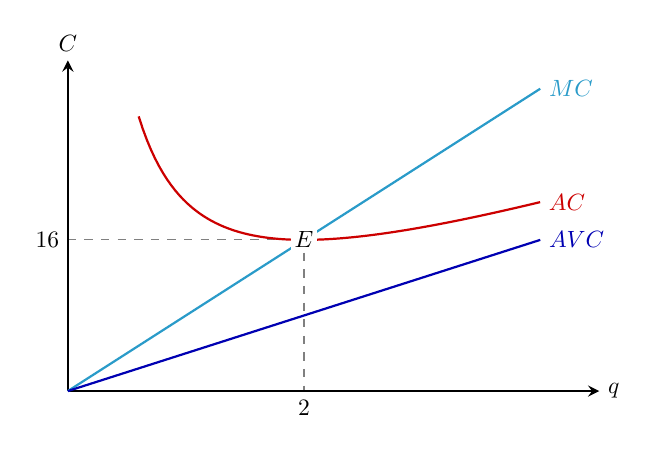
\begin{tikzpicture}[x=1.5cm, y=0.12cm, >=stealth, thick, every node/.style={scale=0.85}]
				% 1. 全局辅助虚线 (置于最底层防遮挡)
				\draw[dashed, gray, thin] (0, 16) -- (2, 16) -- (2, 0);
				
				% 2. 坐标轴
				\draw[->] (0,0) -- (4.5,0) node[right] {$q$};
				\draw[->] (0,0) -- (0,35) node[above] {$C$};
				
				% 3. 核心数学曲线绘制 (严格裁切定义域防溢出)
				\draw[cyan!80!black, domain=0:4] plot (\x, {8*\x}) node[right] {$MC$};
				\draw[blue!70!black, domain=0:4] plot (\x, {4*\x}) node[right] {$AVC$};
				\draw[red!80!black, domain=0.6:4, samples=100] plot (\x, {16/\x + 4*\x}) node[right] {$AC$};
				
				% 4. 标签与交点标注
				\node[fill=white, inner sep=1.5pt] at (2,16) {$E$};
				\node[left] at (0,16) {$16$};
				\node[below] at (2,0) {$2$};
			\end{tikzpicture}
		\end{center}
		
		\item \textbf{一家竞争性厂商的短期成本函数为 $C(q) = q^3 - 8q^2 + 30q + 5$。请推导边际成本、平均成本和平均可变成本并在图形上标示。分析当价格处于何种区间时厂商产量为零，在图上勾勒厂商的供给曲线，并计算当产量为 6 时所需的市场价格。}
		
		\textbf{答：}
		首先，对总成本函数求导并运用均摊法则，可分别推导出边际成本 $MC = 3q^2 - 16q + 30$、平均可变成本 $AVC = q^2 - 8q + 30$ 以及平均成本 $AC = q^2 - 8q + 30 + 5/q$。其次，厂商在短期内维持生产的物理底线是价格不低于 $AVC$ 的最低点（即短期停业点）。通过联立 $MC = AVC$ 搜寻该临界点：
		\[
		\begin{aligned}
			3q^2 - 16q + 30 &= q^2 - 8q + 30 \\
			2q^2 - 8q &= 0
		\end{aligned}
		\]
		解得停业临界产量 $q = 4$。将其反代入 $AVC$ 函数，得到最低可变成本 $AVC_{min} = 14$。这意味着，当市场价格处于 $P < 14$ 区间时，厂商连基本的可变成本都无法弥补，理性的选择是瞬间停产，产量归零。再者，当超越该停业点后，向右上方倾斜的边际成本曲线片段（图中点 $A$ 右侧的加粗红线段）在几何上严格映射为厂商的短期供给曲线。最终，依据 $P = MC$ 的利润最大化原则，若要使厂商提供 6 个单位的产量，市场价格必须被精准锁定在：
		\[
		\begin{aligned}
			P &= 3 \times 6^2 - 16 \times 6 + 30 = 42
		\end{aligned}
		\]
		
		\begin{center}
			\begin{tikzpicture}[x=1.5cm, y=0.12cm, >=stealth, thick, every node/.style={scale=0.85}]
				% 1. 全局辅助虚线 (置于最底层防遮挡)
				\draw[dashed, gray, thin] (0, 14) -- (4, 14) -- (4, 0);
				\draw[dashed, gray, thin] (0, 42) -- (6, 42) -- (6, 0);
				
				% 2. 坐标轴
				\draw[->] (0,0) -- (7.5,0) node[right] {$q$};
				\draw[->] (0,0) -- (0,55) node[above] {$C, P$};
				
				% 3. 核心数学曲线绘制 (严格裁切定义域，手动锚定标签防堆叠)
				% AVC 曲线
				\draw[cyan!80!black, domain=1:6.8, samples=100] plot (\x, {\x*\x - 8*\x + 30});
				\node[cyan!80!black, right] at (6.8, {6.8*6.8 - 8*6.8 + 30 - 1.5}) {$AVC$}; % 标签刻意向下偏移
				
				% AC 曲线 (由于 AC = AVC + 5/q，在大产量时两线必然数学趋近。此处微调标签位置以错开视觉重叠)
				\draw[blue!70!black, domain=1.2:6.8, samples=100] plot (\x, {\x*\x - 8*\x + 30 + 5/\x});
				\node[blue!70!black, right] at (6.8, {6.8*6.8 - 8*6.8 + 30 + 5/6.8 + 1.5}) {$AC$}; % 标签刻意向上偏移
				
				% 边际成本分为两段绘制：低于停业点的为普通线，高于停业点的加粗变色作为供给曲线
				\draw[gray, domain=1.5:4, samples=50] plot (\x, {3*\x*\x - 16*\x + 30});
				\draw[red!80!black, line width=1.2pt, domain=4:6.3, samples=100] plot (\x, {3*\x*\x - 16*\x + 30});
				\node[red!80!black, above left] at (6.3, {3*6.3*6.3 - 16*6.3 + 30}) {$MC \, (\text{供给曲线})$};
				
				% 4. 标签与交点标注
				\node[fill=white, inner sep=1.5pt] at (4,14) {$A$};
				\node[left] at (0,14) {$14$};
				\node[below] at (4,0) {$4$};
				\node[left] at (0,42) {$42$};
				\node[below] at (6,0) {$6$};
			\end{tikzpicture}
		\end{center}
		
		\item \textbf{假设某厂商的生产函数为 $q = 9x^{1/2}$，在短期内，固定成本为 1000 美元，可变投入 $x$ 的单位成本为 4000 美元。请推导出生产 $q$ 单位产品的总成本函数并写出供给曲线方程。如果市场价格跃升至 1000 美元，厂商的产量和利润水平将达到多少？并在成本曲线图上标示出结论。}
		
		\textbf{答：}
		对生产函数进行逆推，得可变要素需求量 $x = q^2/81$。将其与要素价格相乘，并叠加恒定的固定成本，即可获得关于产出的二次总成本函数：
		\[
		\begin{aligned}
			C(q) &= FC + P_{x} \cdot x \\
			&= 1000 + 4000 \left(\frac{q^2}{81}\right) = \frac{4000}{81}q^2 + 1000
		\end{aligned}
		\]
		其次，基于完全竞争法则，厂商的短期供给曲线等同于边际成本曲线。由此，厂商的线性供给曲线方程直接确立为 $P = 8000q/81 \, (q>0)$。再者，当遭遇 1000 美元的价格信号冲击时，将价格代入供给方程：
		\[
		\begin{aligned}
			1000 &= \frac{8000q}{81} \\
			q &= 10.125
		\end{aligned}
		\]
		最终，利润等于总收益减去总成本。将最优产量回代至利润表达式中进行核算：
		\[
		\begin{aligned}
			\pi &= TR - TC \\
			&= 1000 \times 10.125 - \left[\frac{4000}{81} \times (10.125)^{2} + 1000\right] \\
			&= 10125 - (5062.5 + 1000) = 4062.5 \, \text{（美元）}
		\end{aligned}
		\]
		在几何图面上，如图所示，这笔高达 4062.5 美元的超额利润，被精确映射为夹在市场价格线（$P=1000$）与平均成本曲线交点（$AC \approx 598.7$）之间，且宽度延展至均衡产量 $10.125$ 的浅色阴影矩形块。
		
		\begin{center}
			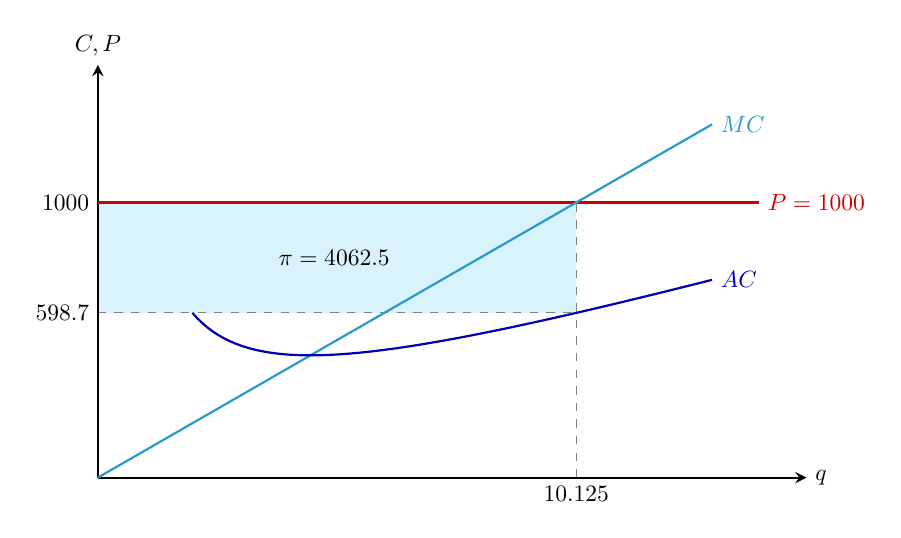
\begin{tikzpicture}[x=0.6cm, y=0.0035cm, >=stealth, thick, every node/.style={scale=0.85}]
				% 1. 阴影面积填充 (置于底层防遮挡) 
				% 10.125 处的 AC 大约为 598.76
				\fill[cyan!15] (0, 598.76) rectangle (10.125, 1000);
				
				% 2. 坐标轴与辅助线
				\draw[dashed, gray, thin] (10.125, 0) -- (10.125, 1000);
				\draw[dashed, gray, thin] (0, 598.76) -- (10.125, 598.76);
				\draw[->] (0,0) -- (15,0) node[right] {$q$};
				\draw[->] (0,0) -- (0,1500) node[above] {$C, P$};
				
				% 3. 核心曲线绘制
				\draw[red!80!black] (0, 1000) -- (14, 1000) node[right] {$P=1000$};
				% 修复：加括号改变运算顺序，避免 8000*\x 内部计算超过 16384 的上限
				\draw[cyan!80!black, domain=0:13] plot (\x, {(8000/81)*\x}) node[right] {$MC$};
				% 修复：同理处理 4000*\x
				\draw[blue!70!black, domain=2:13, samples=100] plot (\x, {(4000/81)*\x + 1000/\x}) node[right] {$AC$};
				
				% 4. 标签与交点标注
				\node at (5, 800) {$\pi = 4062.5$};
				\node[left] at (0,1000) {$1000$};
				\node[left] at (0,598) {$598.7$};
				\node[below] at (10.125,0) {$10.125$};
			\end{tikzpicture}
		\end{center}
		
		\item \textbf{假设某一特殊行业的市场需求为 $Q^D = 6500 - 100P$，市场供给为 $Q^S = 1200P$。行业内所有厂商完全相同且处于完全竞争状态，单家厂商的总成本为 $C(q) = 722 + q^2/200$，边际成本为 $MC(q) = 2q/200$。请计算当期均衡指标，并详细分析行业的长期进退动态以及短/长期的底线销售价格。}
		
		\textbf{答：}
		首先，联立市场需求与供给方程可求得当期市场均衡指标。由 $6500 - 100P = 1200P$ 解得市场均衡价格 $P = 5$，代入可得行业总产量 $Q = 6000$。在完全竞争市场中，厂商依据价格等于边际成本（$P = MC$）原则实现利润最大化，即：
		\[
		\begin{aligned}
			5 = \frac{q}{100} \implies q = 500
		\end{aligned}
		\]
		此时行业内生产的厂商数量为 $N = Q/q = 12$ 家，单家厂商所获经济利润为 $\pi = 5 \times 500 - (722 + 500^2/200) = 528$。
		
		其次，分析行业的长期进退动态。由于当前存在正的经济利润（$\pi = 528$），在长期会吸引外部新厂商进入该行业。随着厂商数量增加，行业供给曲线将向右下方移动，导致市场均衡价格不断压低，直至单家厂商的超额经济利润被完全榨干，行业达到长期的稳态均衡。
		
		再者，行业的长期底线销售价格取决于平均成本（$AC$）的最低点。令边际成本等于平均成本以求取长期均衡状态下的厂商产量与价格底线：
		\[
		\begin{aligned}
			\frac{722}{q} + \frac{q}{200} &= \frac{q}{100} \\
			\frac{q}{200} &= \frac{722}{q} \implies q = 380
		\end{aligned}
		\]
		将长期底线产量 $q = 380$ 代入，求得长期的绝对底线价格 $P_{LR} = AC(380) = 3.8$。当价格低于 $3.8$ 时，厂商在长期将亏损并选择退出行业。
		
		最终，在短期内厂商维持生产的底线是价格不低于最低平均可变成本（$\min AVC$）。由于本题中可变成本为 $VC = q^2/200$，其平均可变成本为 $AVC = q/200$。当产量 $q$ 趋近于零时，$AVC$ 的谷底极限值为 $0$。因此，在短期内只要价格微大于零，厂商继续生产所获得的收益便能部分弥补固定成本，故短期的底线销售价格理论上趋于 $0$。

		
		\item \textbf{竞争性厂商的总成本函数为 $C(q) = 450 + 15q + 2q^{2}$，边际成本函数为 $MC(q) = 15 + 4q$。如果市场价格为 $P=115$ 美元/单位，求出厂商生产的产量，并计算利润和生产者剩余。}
		
		\textbf{答：}
		首先，竞争性厂商通过将边际成本与给定的市场价格对齐来搜寻最优产出规模。构建一阶利润最大化条件 $P = MC$，即 $115 = 15 + 4q$，通过简单的代数移项可解得厂商的最优产量为 $q = 25$。其次，将该产量代入总收益与总成本之差的等式中，可核算出厂商当期截获的绝对经济利润：
		\[
		\begin{aligned}
			\pi &= P q - C(q) \\
			&= 115 \times 25 - \left(450 + 15 \times 25 + 2 \times 25^{2}\right) \\
			&= 2875 - (450 + 375 + 1250) = 800 \, \text{（美元）}
		\end{aligned}
		\]
		最终，考察该厂商的生产者剩余。从代数逻辑上看，生产者剩余等于总收益剥离总可变成本，亦等价于经济利润加上固定成本。从几何形态上看，如图所示，由于边际成本曲线呈完美线性，生产者剩余严格映射为市场价格线与边际成本曲线之间所夹的阴影三角形面积。两种路径的计算殊途同归：
		\[
		\begin{aligned}
			PS &= \pi + FC = 800 + 450 = 1250 \, \text{（美元）} \\
			PS &= \frac{1}{2} \times (115 - 15) \times 25 = 1250 \, \text{（美元）}
		\end{aligned}
		\]
		
		\begin{center}
			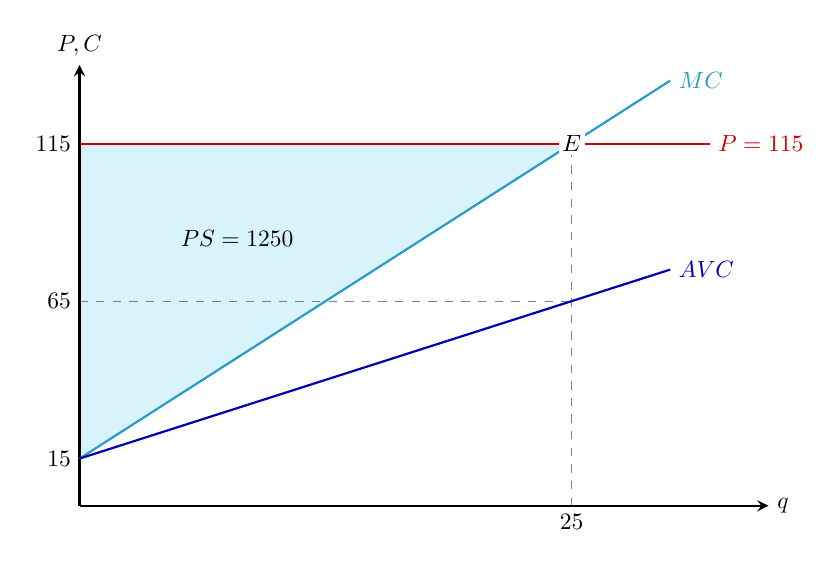
\begin{tikzpicture}[x=0.25cm, y=0.04cm, >=stealth, thick, every node/.style={scale=0.85}]
				% 1. 阴影填充 (底层)
				\fill[cyan!15] (0,15) -- (25,115) -- (0,115) -- cycle;
				
				% 2. 辅助线
				\draw[dashed, gray, thin] (25,0) -- (25,115);
				\draw[dashed, gray, thin] (0,65) -- (25,65);
				
				% 3. 坐标轴
				\draw[->] (0,0) -- (35,0) node[right] {$q$};
				\draw[->] (0,0) -- (0,140) node[above] {$P, C$};
				
				% 4. 核心曲线绘制
				\draw[red!80!black] (0,115) -- (32,115) node[right] {$P=115$};
				\draw[cyan!80!black, domain=0:30] plot (\x, {15 + 4*\x}) node[right] {$MC$};
				\draw[blue!70!black, domain=0:30] plot (\x, {15 + 2*\x}) node[right] {$AVC$};
				
				% 5. 标签防遮挡锚定
				\node[fill=white, inner sep=1.5pt] at (25,115) {$E$};
				\node at (8, 85) {$PS = 1250$};
				\node[left] at (0,115) {$115$};
				\node[left] at (0,65) {$65$};
				\node[left] at (0,15) {$15$};
				\node[below] at (25,0) {$25$};
			\end{tikzpicture}
		\end{center}
		
		\item \textbf{很多商店提供相片冲洗服务。如果每家商店的成本函数均为 $C(q) = 50 + 0.5q + 0.08q^2$，边际成本为 $MC(q) = 0.5 + 0.16q$。如果当前收费为 8.50 美元，该行业处在长期均衡状态吗？若不是，长期均衡价格是多少？假设新冲洗技术可使成本整体降低 25\%，在行业处于长期均衡时，厂商最多愿意支付多高的价格购买该技术？}
		
		\textbf{答：}
		首先，检验当前 8.50 美元价格下的行业状态。根据利润最大化条件 $P = MC$，将 $P = 8.5$ 代入边际成本函数解得最优产量 $q = 50$。此时单家厂商所获的经济利润为：
		\[
		\begin{aligned}
			\pi &= 8.5 \times 50 - \left[50 + 0.5 \times 50 + 0.08 \times (50)^2\right] \\
			&= 425 - 275 = 150 \text{（美元）}
		\end{aligned}
		\]
		由于此时存在严格为正的经济利润（如图中 $A$ 点所示），行业将吸引新厂商进入，因此当前并不处于长期均衡状态。
		
		在长期动态演化中，新厂商的进入会增加市场供给并压低价格。长期均衡的达成条件是超额经济利润被完全消除，此时市场价格必须等于平均成本曲线的最底端（即满足 $MC = AC$ 的临界点）：
		\[
		\begin{aligned}
			0.5 + 0.16q &= \frac{50}{q} + 0.5 + 0.08q \\
			0.08q^2 &= 50 \implies q = 25
		\end{aligned}
		\]
		由此推导出，该行业的长期均衡价格为 $P = MC(25) = 4.5$ 美元，对应图中的 $E_1$ 点。
		
		当厂商引入降低 25\% 成本的新技术后，其总成本函数更新为 $C_{new}(q) = 37.5 + 0.375q + 0.06q^2$，相应的边际成本下移为 $MC_{new} = 0.375 + 0.12q$。如图所示，新技术的采用使得该厂商的平均成本曲线由 $AC_1$ 下移至 $AC_2$，边际成本曲线由 $MC_1$ 下移至 $MC_2$。若市场价格仍处于原长期均衡位势（$P = 4.5$），率先采用该技术的厂商将依据新的边际成本曲线重新设定产量至 $E_2$ 点：
		\[
		\begin{aligned}
			4.5 &= 0.375 + 0.12q \implies q = 34.375
		\end{aligned}
		\]
		
		最终，将新的最优产量 $34.375$ 代入新成本结构，核算该厂商由于技术红利所能获得的经济利润：
		\[
		\begin{aligned}
			\pi_{new} &= 4.5 \times 34.375 - \left[37.5 + 0.375 \times 34.375 + 0.06 \times (34.375)^2\right] \\
			&= 154.6875 - 121.2891 \approx 33.40 \text{（美元）}
		\end{aligned}
		\]
		由于引入新技术前厂商在长期均衡状态下的经济利润为零，这笔约 33.40 美元的额外经济利润，便构成了该厂商为购买该项技术专利所愿意支付的最高对价。
		
		\begin{center}
			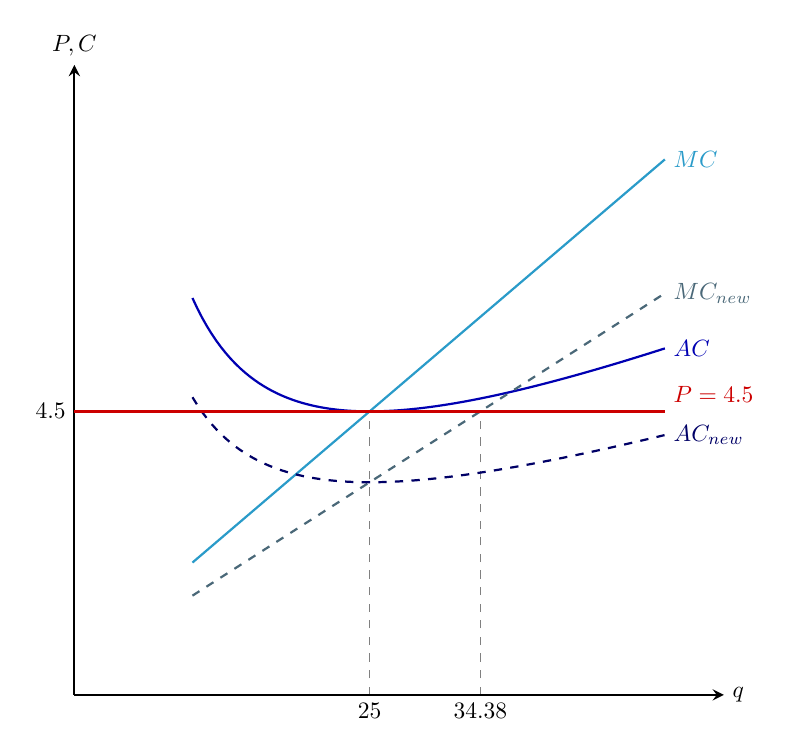
\begin{tikzpicture}[x=0.15cm, y=0.8cm, >=stealth, thick, every node/.style={scale=0.85}]
				% 1. 辅助虚线
				\draw[dashed, gray, thin] (25,0) -- (25,4.5);
				\draw[dashed, gray, thin] (34.375,0) -- (34.375,4.5);
				
				% 2. 坐标轴
				\draw[->] (0,0) -- (55,0) node[right] {$q$};
				\draw[->] (0,0) -- (0,10) node[above] {$P, C$};
				
				% 3. 原成本曲线
				\draw[cyan!80!black, domain=10:50] plot (\x, {0.5 + 0.16*\x}) node[right] {$MC$};
				\draw[blue!70!black, domain=10:50, samples=100] plot (\x, {50/\x + 0.5 + 0.08*\x}) node[right] {$AC$};
				
				% 4. 新成本曲线 (技术进步)
				\draw[cyan!40!black, dashed, domain=10:50] plot (\x, {0.375 + 0.12*\x}) node[right] {$MC_{new}$};
				\draw[blue!40!black, dashed, domain=10:50, samples=100] plot (\x, {37.5/\x + 0.375 + 0.06*\x}) node[right] {$AC_{new}$};
				
				% 5. 均衡价格线与标签
				\draw[red!80!black] (0,4.5) -- (50,4.5) node[above right] {$P=4.5$};
				\node[left] at (0,4.5) {$4.5$};
				\node[below] at (25,0) {$25$};
				\node[below] at (34.375,0) {$34.38$};
			\end{tikzpicture}
		\end{center}
		\newpage
		\item \textbf{假设某城市市中心的热狗销售亭边际成本均为 1.50 美元/个，无固定成本，且面临每天最多销售 100 个的产能天花板。如果当前售价 2 美元，每家想销售多少？该完全竞争状态下的 2 美元能否长期持续？若市场需求为 $Q = 4400 - 1200P$，均衡时有多少家销售亭？若政府无偿限发 20 个许可证，销售价格和牌照的最大支付意愿各是多少？}
		
		\textbf{答：}
		首先，在 2 美元的市场价格下，由于单家厂商面临的边际收益（2 美元）严格大于边际成本（1.5 美元），利润最大化将驱使销售亭满负荷运转。受限于刚性的产能天花板，其最优日销售量处于 $q = 100$ 个的角点解。
		
		在无进入壁垒的完全竞争生态中，2 美元的价格无法在长期维持。单件 0.5 美元的正向利润空间将吸引新厂商进入市场，总供给的增加会导致市场均衡价格下行，直至价格收敛于边际成本，即长期均衡价格为 $P = 1.5$ 美元。
		
		如图 (a) 所示，当市场在长期底线出清时，将 $P = 1.5$ 代入市场需求函数，可得均衡总成交量：
		\[
		\begin{aligned}
			Q &= 4400 - 1200 \times 1.5 = 2600
		\end{aligned}
		\]
		按照每家销售亭满载 100 个计算，长期均衡状态下市场将容纳 $N = 2600 / 100 = 26$ 家厂商，对应图中 $E_1$ 点。
		
		最终，若市政当局实施配额干预，将特许经营牌照限制在 20 张，市场的总供给量将被强制截断在垂直的供给线 $S_{quota} = 20 \times 100 = 2000$ 个。将此配额供给量代入需求函数以求取新的市场出清价格：
		\[
		\begin{aligned}
			2000 &= 4400 - 1200P \implies P = 2 \text{（美元）}
		\end{aligned}
		\]
		在配额制度下（图中 $E_2$ 点），热狗售价回升至 2 美元。此时，拥有牌照的单家销售亭每天可获得超额经济利润 $\pi = 100 \times (2 - 1.5) = 50$ 美元。这笔每日 50 美元的稳定经济地租，即构成了理性厂商为争夺该经营许可证所愿意支付的最大竞价。
		
		\begin{center}
			\begin{tikzpicture}[>=stealth, thick, every node/.style={scale=0.85}, x=0.0022cm, y=1.2cm]
				% 全局投影虚线
				\draw[dashed, gray, thin] (0, 2) -- (2000, 2) -- (2000, 0);
				\draw[dashed, gray, thin] (0, 1.5) -- (2600, 1.5) -- (2600, 0);
				
				% 坐标轴
				\draw[->] (0,0) -- (3500,0) node[right] {$Q$};
				\draw[->] (0,0) -- (0,3.5) node[above] {$P$};
				\node[below left] at (0,0) {$0$};
				
				% 需求与供给曲线
				\draw[draw=blue, domain=500:3200, smooth] plot (\x, {44/12 - \x/1200}) node[right] {$D$};
				\draw[draw=orange, domain=0:3200] plot (\x, {1.5}) node[above] {$S_{LR}$};
				\draw[draw=red, domain=0:3] (2000, 0) -- (2000, 3) node[right] {$S_{quota}$};
				
				% 交点与标号
				\fill (2600, 1.5) circle (1.5pt);
				\node[above right, fill=white, inner sep=1pt] at (2600, 1.5) {$E_1$};
				\node[below, text=black] at (2600, 0) {$2600$};
				\node[left, text=black] at (0, 1.5) {$1.5$};
				
				\fill (2000, 2) circle (1.5pt);
				\node[above right, fill=white, inner sep=1pt] at (2000, 2) {$E_2$};
				\node[below, text=black] at (2000, 0) {$2000$};
				\node[left, text=black] at (0, 2) {$2$};
				
				\node[below] at (1500, -0.6) {(a) 热狗市场总供需与配额效应};
			\end{tikzpicture}
		\end{center}
		\newpage
		\item \textbf{对竞争性行业中的一个售价为 5 美元的产品厂商开征 1 美元的销售税。该孤立税收如何扭曲该厂商的成本曲线？厂商的价格、产出与利润将发生何种异动？长期来看，该厂商是坚守还是逃离？}
		
		\textbf{答：}
		该笔仅针对单一厂商征收的 1 美元专属销售税，在数学几何上等效于将其总成本曲线整体向上平移。这将直接导致其平均成本曲线上移至 $AC_{tax} = AC + 1$，边际成本曲线也同步上移至 $MC_{tax} = MC + 1$。
		
		在完全竞争市场中，单个厂商是宏观价格的被动接受者。由于全行业仅有该单一厂商被征税，其个体的产量缩减不足以影响市场总供给，因此厂商面临的外部销售价格将维持在 $P = 5$ 美元不变。如图 (b) 所示，在成本曲线上移的压迫下，为了重新满足 $P = MC_{tax}$ 的利润最大化条件，厂商的最优产量点将由 $E_1$ 沿着新的边际成本曲线左移至 $E_2$，产出不可避免地出现缩减。与此同时，由于价格被锁定而平均成本全面抬升，厂商的利润空间被严重挤压并陷入负值区域。
		
		考量长期的市场演化。在完全竞争的稳态下，原生厂商本身处于 $P = \min AC$ 的零经济利润均衡点。这 1 美元的额外税负使得厂商税后的最低平均成本严格高于市场价格（$\min AC_{tax} > P$）。面对长期中无法消除的绝对亏损，理性的经济决策注定该厂商将被迫清算资产，永久性地退出该行业。
		
		\begin{center}
			\begin{tikzpicture}[>=stealth, thick, every node/.style={scale=0.85}, x=0.4cm, y=0.6cm]
				% 全局投影虚线
				\draw[dashed, gray, thin] (0, 5) -- (12, 5);
				\draw[dashed, gray, thin] (8, 0) -- (8, 6.125);
				\draw[dashed, gray, thin] (10, 0) -- (10, 5);
				\draw[dashed, gray, thin] (0, 6.125) -- (8, 6.125);
				
				% 坐标轴
				\draw[->] (0,0) -- (15,0) node[right] {$q$};
				\draw[->] (0,0) -- (0,8.5) node[above] {$P, C$};
				\node[below left] at (0,0) {$0$};
				
				% 价格线
				\draw[draw=black] (0, 5) -- (14, 5) node[right] {$P=5$};
				
				% 原成本曲线 (设定 MC = 0.5q, AC = 0.25q + 25/q， min AC = 5 在 q=10)
				\draw[draw=blue, domain=4.5:14, smooth] plot (\x, {0.25*\x + 25/\x}) node[right] {$AC_1$};
				\draw[draw=cyan!80!black, domain=0:14, smooth] plot (\x, {0.5*\x}) node[right] {$MC_1$};
				
				% 税后成本曲线 (上移 1 个单位)
				\draw[draw=red, domain=4.5:14, smooth] plot (\x, {0.25*\x + 25/\x + 1}) node[right] {$AC_{tax}$};
				\draw[draw=orange!90!red, domain=0:14, smooth] plot (\x, {0.5*\x + 1}) node[right] {$MC_{tax}$};
				
				% 交点与标号
				\fill (10, 5) circle (1.5pt);
				\node[below right, fill=white, inner sep=1pt] at (10, 5) {$E_1$};
				\node[below, text=black] at (10, 0) {$q_1$};
				
				\fill (8, 5) circle (1.5pt);
				\node[below right, fill=white, inner sep=1pt] at (8, 5) {$E_2$};
				\node[below, text=black] at (8, 0) {$q_2$};
				
				\fill (8, 6.125) circle (1.5pt);
				\node[left, text=black] at (0, 6.125) {$AC_2$};
				\node[left, text=black] at (0, 5) {$5$};
				
				\node[below] at (7, -1.2) {(b) 单一厂商的征税效应与退出动态};
			\end{tikzpicture}
		\end{center}
		\newpage
		\item \textbf{在一竞争性行业中，一半的环境污染厂商被征收 10\% 销售税，税收全额转用作对另一半无污染厂商的 10\% 销售补贴。假设初态所有厂商长期平均成本相同，长短期内各变量将如何演化？这种完美的税补预算平衡政策能否长久维系？}
		
		\textbf{答：}
		首先，分析短期的产量与价格调整。征收 10\% 的税收使污染厂商的成本曲线整体上移，而 10\% 的补贴使清洁厂商的成本曲线对称下移。如图 (a) 与 (b) 所示，在初始市场均衡价格 $P_0$ 下，污染厂商依据 $P_0 = MC_t$ 将最优产量由 $q_0$ 缩减至 $q_1$；清洁厂商则依据 $P_0 = MC_s$ 将产量由 $q_0$ 扩张至 $q_2$。由于双方初始规模对称且成本平移幅度相同，个体产量的增减相互抵消（$\Delta q_p + \Delta q_c = 0$）。因此，短期内行业总供给保持不变，市场出清价格维持在 $P_0$。
		
		接着分析长期的行业进退动态。在价格 $P_0$ 下，污染厂商因平均成本高于价格（$AC_t > P_0$）而遭受经济亏损，将逐渐退出市场；清洁厂商因平均成本低于价格（$AC_s < P_0$）获得超额利润，从而吸引新资本进入。长期来看，污染厂商将被完全淘汰，市场结构彻底转变为全清洁产能。
		
		最终，检验该预算平衡政策的长期可持续性。若政府需维持财政收支平衡，必须满足税收等于补贴的约束：
		\[
		\begin{aligned}
			t \cdot P \cdot Q_p &= s \cdot P \cdot Q_c \implies s = t \left( \frac{Q_p}{Q_c} \right)
		\end{aligned}
		\]
		式中 $Q_p$ 与 $Q_c$ 分别代表污染与清洁厂商的总产量。随着污染厂商退出（$Q_p \to 0$）与清洁厂商扩张，在固定税率 $t$ 下，政府必须持续下调补贴率 $s$ 以维持收支平衡。当行业完全由清洁厂商构成时（$Q_p = 0$），税收总额归零，补贴率 $s$ 必然降至零。此时税补政策自然终止，留存厂商的成本曲线回落至初始状态，市场将以原价格 $P_0$ 达成全新的长期零利润均衡。
		
		\begin{center}
			\begin{tikzpicture}[>=stealth, thick, every node/.style={scale=0.85}, x=0.55cm, y=0.32cm]
				% ------------------ 层 0: 全局价格投影虚线 ------------------
				\draw[dashed, gray, thin] (0, 8) -- (16.5, 8);
				\node[left, text=black] at (0, 8) {$P_0$};
				
				% ------------------ 层 1: 左图 (污染厂商) ------------------
				\begin{scope}[xshift=0cm]
					% 坐标轴
					\draw[->] (0,0) -- (7.5,0) node[right] {$q$};
					\draw[->] (0,0) -- (0,14) node[above] {$P, C$};
					\node[below left] at (0,0) {$0$};
					
					% 原初成本曲线 (AC = q + 16/q, MC = 2q)
					\draw[draw=blue, domain=1.8:6.5, smooth] plot (\x, {\x + 16/\x});
					\draw[draw=cyan!80!black, domain=0:6.5, smooth] plot (\x, {2*\x});
					
					% 征税后成本曲线 (上移 2 个单位)
					\draw[draw=red, domain=1.8:6.5, smooth] plot (\x, {\x + 16/\x + 2}) node[right] {$AC_t$};
					\draw[draw=orange!90!red, domain=0:5.5, smooth] plot (\x, {2*\x + 2}) node[right] {$MC_t$};
					
					% 交点与标号
					\fill (4, 8) circle (1.5pt);
					\node[below right, fill=white, inner sep=1pt] at (4, 8) {$E_0$};
					\draw[dashed, gray, thin] (4,0) node[below] {$q_0$} -- (4,8);
					
					\fill (3, 8) circle (1.5pt);
					\node[above left, fill=white, inner sep=1pt] at (3, 8) {$E_1$};
					\draw[dashed, gray, thin] (3,0) node[below] {$q_1$} -- (3,8);
					
					\node[below] at (3.75, -1.8) {(a) 污染厂商减产与亏损};
				\end{scope}
				
				% ------------------ 层 2: 右图 (清洁厂商) ------------------
				\begin{scope}[xshift=5.2cm] 
					% 坐标轴
					\draw[->] (0,0) -- (7.5,0) node[right] {$q$};
					\draw[->] (0,0) -- (0,14) node[above] {$P, C$};
					\node[below left] at (0,0) {$0$};
					
					% 原初成本曲线
					\draw[draw=blue, domain=1.8:6.5, smooth] plot (\x, {\x + 16/\x});
					\draw[draw=cyan!80!black, domain=0:6.5, smooth] plot (\x, {2*\x});
					
					% 补贴后成本曲线 (下移 2 个单位)
					\draw[draw=green!60!black, domain=2:6.5, smooth] plot (\x, {\x + 16/\x - 2}) node[right] {$AC_s$};
					\draw[draw=teal, domain=0:7, smooth] plot (\x, {2*\x - 2}) node[above right] {$MC_s$};
					
					% 交点与标号
					\fill (4, 8) circle (1.5pt);
					\node[above left, fill=white, inner sep=1pt] at (4, 8) {$E_0$};
					\draw[dashed, gray, thin] (4,0) node[below] {$q_0$} -- (4,8);
					
					\fill (5, 8) circle (1.5pt);
					\node[below right, fill=white, inner sep=1pt] at (5, 8) {$E_2$};
					\draw[dashed, gray, thin] (5,0) node[below] {$q_2$} -- (5,8);
					
					\node[below] at (3.75, -1.8) {(b) 清洁厂商扩张与盈利};
				\end{scope}
			\end{tikzpicture}
		\end{center}
	\end{enumerate}
	
	% =======================================================
	%                   第 9 章：竞争性市场分析
	% =======================================================
	\chapter{竞争性市场分析}
	
	\section{复习题}
	\begin{enumerate}[label=\textbf{\arabic*.}, leftmargin=*]
		\item \textbf{无谓损失的含义是什么？为什么价格上限通常导致无谓损失？}
		
		\textbf{答：}
		首先，无谓损失是指市场在偏离竞争性均衡的非效率状态下，生产者与消费者总剩余的净减少量，即任何一方都未能获得的福利。其次，价格上限管制导致无谓损失的机制如下。
		
		如图所示，当政府设定低于市场均衡价格 $P_0$ 的价格上限 $P_{max}$ 时，市场有效交易量由 $Q_0$ 减少至 $Q_1$。对于仍能以低价购得商品的消费者，其消费者剩余增加了矩形 $A$ 的面积；但由于产出减少，部分需求无法满足，产生面积为 $B$ 的福利损失。对于生产者，由于价格下降且产出减少，其生产者剩余的损失包括向消费者转移的矩形 $A$ 以及产出减少造成的三角形 $C$。相关的福利变动可量化为：
		\[
		\begin{aligned}
			\Delta CS &= A - B \\
			\Delta PS &= -A - C \\
			\Delta TS &= \Delta CS + \Delta PS = -(B + C)
		\end{aligned}
		\]
		最终，社会总剩余（$\Delta TS$）的净损失为图中的三角形 $B$ 与 $C$ 之和，这确切地映射了价格上限所引发的无谓损失。
		
		\begin{center}
			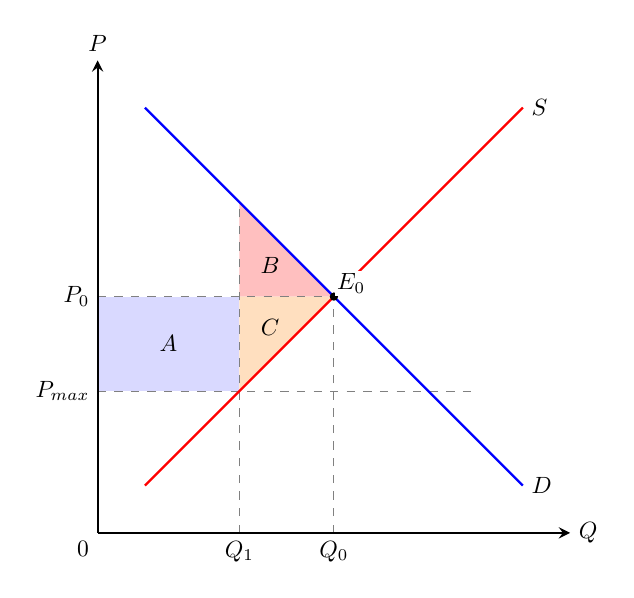
\begin{tikzpicture}[x=0.6cm, y=0.6cm, >=stealth, thick, every node/.style={scale=0.85}]
				% 1. 福利或剩余区域填充 (最底层)
				\fill[blue!15] (0, 3) rectangle (3, 5);
				\node at (1.5, 4) {$A$};
				\fill[red!25] (3, 5) -- (3, 7) -- (5, 5) -- cycle;
				\node at (3.65, 5.65) {$B$};
				\fill[orange!25] (3, 3) -- (3, 5) -- (5, 5) -- cycle;
				\node at (3.65, 4.35) {$C$};
				
				% 2. 全局辅助虚线
				\draw[dashed, gray, thin] (0, 5) node[left, text=black] {$P_0$} -- (5, 5);
				\draw[dashed, gray, thin] (5, 0) node[below, text=black] {$Q_0$} -- (5, 5);
				\draw[dashed, gray, thin] (0, 3) node[left, text=black] {$P_{max}$} -- (8, 3);
				\draw[dashed, gray, thin] (3, 0) node[below, text=black] {$Q_1$} -- (3, 7);
				
				% 3. 坐标轴
				\draw[->] (0,0) -- (10,0) node[right] {$Q$};
				\draw[->] (0,0) -- (0,10) node[above] {$P$};
				\node[below left] at (0,0) {$0$};
				
				% 4. 绘图代码
				\draw[draw=blue, domain=1:9, smooth] plot (\x, {10-\x}) node[right] {$D$};
				\draw[draw=red, domain=1:9, smooth] plot (\x, {\x}) node[right] {$S$};
				
				% 5. 均衡点
				\fill (5, 5) circle (1.5pt);
				\node[above right, fill=white, inner sep=1pt] at (5, 5) {$E_0$};
			\end{tikzpicture}
		\end{center}
		\newpage
		\item \textbf{假设某商品的供给曲线完全无弹性。如果政府规定的最高价格低于市场出清价格，这会导致无谓损失吗？请加以解释。}
		
		\textbf{答：}
		首先，供给完全无弹性意味着其价格弹性为零（$E_s = 0$），在几何图形上表现为一条垂直于横轴的供给曲线 $S$，即市场供给量不随价格波动而变化。在此极端条件下，政府设定低于市场出清价格的最高限价并不会导致无谓损失。
		
		如图所示，实施最高限价 $P_{max}$ 后，虽然需求量沿需求曲线 $D$ 扩张至 $Q_1$，但实际交易量受限于刚性供给，依然保持在原均衡产出 $Q_0$ 水平。该政策的实质是一场纯粹的福利转移：价格强制下降使生产者剩余减少了矩形 $A$ 的面积，而这部分福利完全转化为消费者剩余的等量增加。剩余变化如下：
		\[
		\begin{aligned}
			\Delta CS &= A \\
			\Delta PS &= -A \\
			\Delta TS &= \Delta CS + \Delta PS = 0
		\end{aligned}
		\]
		由于市场的总产销量未发生任何实质性萎缩，社会总剩余保持恒定，因此不存在因产出不足而引发的无谓损失（即 $DWL = 0$）。
		
		\begin{center}
			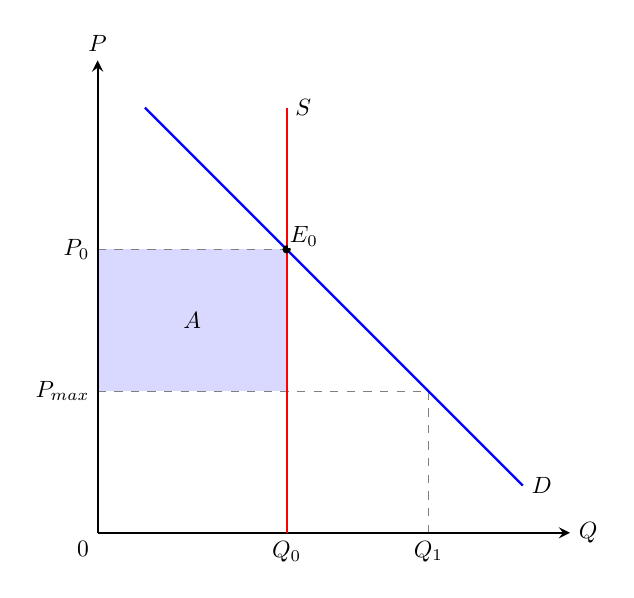
\begin{tikzpicture}[x=0.6cm, y=0.6cm, >=stealth, thick, every node/.style={scale=0.85}]
				% 1. 福利或剩余区域填充
				\fill[blue!15] (0, 3) rectangle (4, 6);
				\node at (2, 4.5) {$A$};
				
				% 2. 全局辅助虚线
				\draw[dashed, gray, thin] (0, 6) node[left, text=black] {$P_0$} -- (4, 6);
				\draw[dashed, gray, thin] (0, 3) node[left, text=black] {$P_{max}$} -- (7, 3);
				\draw[dashed, gray, thin] (7, 0) node[below, text=black] {$Q_1$} -- (7, 3);
				
				% 3. 坐标轴
				\draw[->] (0,0) -- (10,0) node[right] {$Q$};
				\draw[->] (0,0) -- (0,10) node[above] {$P$};
				\node[below left] at (0,0) {$0$};
				
				% 4. 绘图代码
				\draw[draw=blue, domain=1:9, smooth] plot (\x, {10-\x}) node[right] {$D$};
				\draw[draw=red, thick] (4, 0) node[below, text=black] {$Q_0$} -- (4, 9) node[right] {$S$};
				
				% 5. 均衡点
				\fill (4, 6) circle (1.5pt);
				\node[above right, fill=white, inner sep=1pt] at (4, 6) {$E_0$};
			\end{tikzpicture}
		\end{center}
		
		\item \textbf{价格上限怎样改善消费者境况？在什么条件下它可能使消费者的处境变糟？}
		
		\textbf{答：}
		首先，价格上限政策旨在通过限制最高售价来改善消费者的整体福利。当市场供给相对缺乏弹性而需求相对富有弹性时，这一改善效果最为显著，因为价格下调带来的福利转移通常能覆盖产量减少引发的福利损失。然而，当市场供需弹性结构发生反转时，该政策可能使消费者的整体处境恶化。
		
		如图所示，假设市场面临缺乏弹性的需求曲线 $D$ 与富有弹性的供给曲线 $S$。实施价格上限 $P_{max}$ 后，供给量萎缩，市场实际交易量由 $Q_0$ 降至 $Q_1$。对于未能购买到商品而被迫退出市场的消费者，其产生的福利损失为面积较大的深色三角形 $B$；而以低价购得商品的消费者所获得的福利增加，仅为狭长的浅色矩形 $A$。此时，消费者剩余的净变动为：
		\[
		\begin{aligned}
			\Delta CS = A - B < 0
		\end{aligned}
		\]
		在这种极端的数量配给约束下，由于福利损失 $B$ 远大于转移收益 $A$，消费者遭遇了严重的净福利亏损，价格管制反而恶化了需求端的整体处境。
		
		\begin{center}
			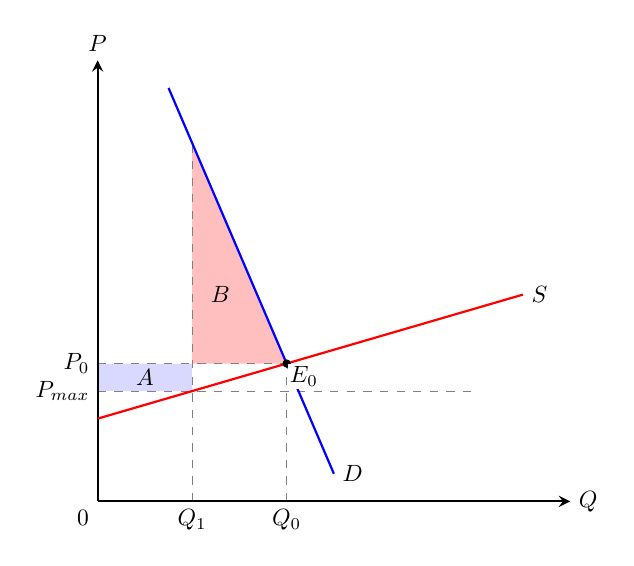
\begin{tikzpicture}[x=0.6cm, y=0.35cm, >=stealth, thick, every node/.style={scale=0.85}]
				% 1. 福利或剩余区域填充 (最底层)
				\fill[blue!15] (0, 4) rectangle (2, 5);
				\node at (1, 4.5) {$A$};
				\fill[red!25] (2, 5) -- (4, 5) -- (2, 13) -- cycle;
				\node at (2.6, 7.5) {$B$};
				
				% 2. 全局辅助虚线
				\draw[dashed, gray, thin] (0, 5) node[left, text=black] {$P_0$} -- (4, 5);
				\draw[dashed, gray, thin] (4, 0) node[below, text=black] {$Q_0$} -- (4, 5);
				\draw[dashed, gray, thin] (0, 4) node[left, text=black] {$P_{max}$} -- (8, 4);
				\draw[dashed, gray, thin] (2, 0) node[below, text=black] {$Q_1$} -- (2, 13);
				
				% 3. 坐标轴
				\draw[->] (0,0) -- (10,0) node[right] {$Q$};
				\draw[->] (0,0) -- (0,16) node[above] {$P$};
				\node[below left] at (0,0) {$0$};
				
				% 4. 绘图代码
				\draw[draw=blue, domain=1.5:5, smooth] plot (\x, {21 - 4*\x}) node[right] {$D$};
				\draw[draw=red, domain=0:9, smooth] plot (\x, {3 + 0.5*\x}) node[right] {$S$};
				
				% 5. 均衡点
				\fill (4, 5) circle (1.5pt);
				\node[below right, fill=white, inner sep=1pt] at (4, 5) {$E_0$};
			\end{tikzpicture}
		\end{center}
		
		\item \textbf{假设政府规定商品的最低价格，这会使生产者整体的处境恶化吗？请加以解释。}
		
		\textbf{答：}
		首先，政府设定高于市场出清水平的最低价格（价格下限）会直接干预市场配给，其对生产者整体处境的负面影响通常体现在两种不同的生产决策情境中。
		
		如图 (a) 所示，在法定的最低价格 $P_{min}$ 约束下，需求端收缩导致市场实际容纳量降至 $Q_1$。若生产者具备完全的信息并选择按需生产（产量控制在 $Q_1$），其能够从消费者处获得等同于矩形 $A$ 的价格转移收益，但同时因销量缩减而承受三角形 $C$ 的福利损失。此时生产者剩余变动取决于 $A$ 与 $C$ 的面积博弈。若市场需求富有弹性，产量的大幅萎缩将导致 $C > A$，从而恶化生产者的整体境况。
		
		其次，现实中更常见且具破坏性的是图 (b) 所示的盲目扩产情境。受高价 $P_{min}$ 的信号诱导，生产者通常会将总产量扩张至 $Q_2$。然而，市场实际消化的成交量仍受限于 $Q_1$，这直接导致了规模为 $Q_2 - Q_1$ 的产品滞销。这部分过剩产出未能转化为任何收入，却确切地消耗了要素投入，其成本总额映射为供给曲线下方的梯形区域 $D$。最终，在存在产能过剩的常态下，生产者剩余的总变动量恶化为：
		\[
		\begin{aligned}
			\Delta PS = A - C - D
		\end{aligned}
		\]
		由于无效生产的沉没成本 $D$ 通常十分庞大，该行业生产者往往会陷入严重的净亏损，其整体境况遭到彻底恶化。
		
		\begin{center}
			\begin{tikzpicture}[x=0.45cm, y=0.45cm, >=stealth, thick, every node/.style={scale=0.85}]
				% ---------- 左图 (a) 按需生产 ----------
				\begin{scope}[xshift=3cm]
					% 1. 区域填充
					\fill[blue!15] (0, 5) rectangle (3, 7);
					\node at (1.5, 6) {$A$};
					\fill[orange!25] (3, 3) -- (3, 5) -- (5, 5) -- cycle;
					\node at (3.65, 4.35) {$C$};
					
					% 2. 辅助虚线
					\draw[dashed, gray, thin] (0, 7) node[left, text=black] {$P_{min}$} -- (7, 7);
					\draw[dashed, gray, thin] (0, 5) node[left, text=black] {$P_0$} -- (5, 5);
					\draw[dashed, gray, thin] (3, 0) node[below, text=black] {$Q_1$} -- (3, 7);
					\draw[dashed, gray, thin] (5, 0) node[below, text=black] {$Q_0$} -- (5, 5);
					
					% 3. 坐标轴
					\draw[->] (0,0) -- (9,0) node[right] {$Q$};
					\draw[->] (0,0) -- (0,9) node[above] {$P$};
					\node[below left] at (0,0) {$0$};
					
					% 4. 曲线
					\draw[draw=blue, domain=1:8, smooth] plot (\x, {10-\x}) node[right] {$D$};
					\draw[draw=red, domain=1:8, smooth] plot (\x, {\x}) node[right] {$S$};
					
					\node[below] at (4.5, -1.5) {(a) 按需生产};
				\end{scope}
				
				% ---------- 右图 (b) 盲目扩产 ----------
				\begin{scope}[xshift=9cm]
					% 1. 区域填充
					\fill[blue!15] (0, 5) rectangle (3, 7);
					\node at (1.5, 6) {$A$};
					\fill[orange!25] (3, 3) -- (3, 5) -- (5, 5) -- cycle;
					\node at (3.65, 4.35) {$C$};
					\fill[gray!30] (3, 0) -- (7, 0) -- (7, 7) -- (3, 3) -- cycle;
					\node at (5.5, 2.5) {$D$};
					
					% 2. 辅助虚线
					\draw[dashed, gray, thin] (0, 7) node[left, text=black] {$P_{min}$} -- (7, 7);
					\draw[dashed, gray, thin] (0, 5) node[left, text=black] {$P_0$} -- (5, 5);
					\draw[dashed, gray, thin] (3, 0) node[below, text=black] {$Q_1$} -- (3, 7);
					\draw[dashed, gray, thin] (7, 0) node[below, text=black] {$Q_2$} -- (7, 7);
					
					% 3. 坐标轴
					\draw[->] (0,0) -- (9,0) node[right] {$Q$};
					\draw[->] (0,0) -- (0,9) node[above] {$P$};
					\node[below left] at (0,0) {$0$};
					
					% 4. 曲线
					\draw[draw=blue, domain=1:8, smooth] plot (\x, {10-\x}) node[right] {$D$};
					\draw[draw=red, domain=1:8, smooth] plot (\x, {\x}) node[right] {$S$};
					
					\node[below] at (4.5, -1.5) {(b) 盲目扩产};
				\end{scope}
			\end{tikzpicture}
		\end{center}
		\newpage
		\item \textbf{现实生活中怎样利用限产来提高下列商品或服务的价格？（1）出租车服务；（2）餐馆或酒吧出售的酒类；（3）小麦或玉米。}
		
		\textbf{答：}
		现实生活中，针对不同商品或服务的特征，政府通常采取差异化的限产机制来干预市场供给，从而提高均衡价格。
		
		首先，针对出租车服务，市政当局通常通过控制营运牌照的发放总额来限制供给。如图 (a) 所示，法定的牌照配额 $Q_{max}$ 将原始供给曲线 $S$ 截断为一条完全无弹性的垂直线（形成折线供给曲线 $S'$）。这种严格的数量配给导致市场均衡由 $E_0$ 移至 $E_1$，服务价格被强制抬高至 $P_1$，从而为既有牌照持有者创造了超额垄断利润。
		
		其次，对于餐馆或酒吧的酒类销售，政府通常通过控制特许经营许可的审批来限制合法的销售终端数量。如图 (b) 所示，营业许可数量的减少使得行业总供给曲线由 $S$ 左移至 $S'$。供给的收缩导致均衡点沿需求曲线 $D$ 向上移动，市场出清价格从 $P_0$ 稳步上升至 $P_1$。
		
		最终，在农产品（如小麦或玉米）市场中，政府通常采用休耕补贴等政策，通过直接的财政转移支付鼓励农场主闲置部分耕地。如图 (c) 所示，休耕政策从生产要素（土地）端限制了产出，使农业供给曲线由 $S$ 左移至 $S'$。更关键的是，初级农作物的需求曲线 $D$ 通常高度缺乏弹性（表现为图形上极为陡峭）。因此，供给的微幅收缩即可促使农产品价格由 $P_0$ 大幅攀升至 $P_1$。由于价格上升的比例远超产量下降的比例，农民的总收益（$TR = P \times Q$）得以实现净增长，从而真正达到托底保收的政策目的。
		
		\begin{center}
			\begin{tikzpicture}[x=0.35cm, y=0.35cm, >=stealth, thick, every node/.style={scale=0.85}]
				
				% ==================== 图 (a): 出租车牌照配额 ====================
				\begin{scope}[xshift=0cm]
					% 辅助线
					\draw[dashed, gray, thin] (0, 4) node[left, text=black] {$P_0$} -- (4, 4);
					\draw[dashed, gray, thin] (4, 0) node[below, text=black] {$Q_0$} -- (4, 4);
					\draw[dashed, gray, thin] (0, 5) node[left, text=black] {$P_1$} -- (3, 5);
					\draw[dashed, gray, thin] (3, 0) node[below, text=black] {$Q_{max}$} -- (3, 7);
					
					% 坐标轴
					\draw[->] (0,0) -- (6,0) node[right] {$Q$};
					\draw[->] (0,0) -- (0,8) node[above] {$P$};
					\node[below left] at (0,0) {$0$};
					
					% 曲线
					\draw[draw=blue, domain=1:6, smooth] plot (\x, {8-\x}) node[right] {$D$};
					\draw[draw=red!40, domain=3:6, dashed] plot (\x, {\x}); % 原始被截断部分
					\draw[draw=red, thick] (0,0) -- (3,3) -- (3, 7.5) node[right] {$S'$}; % 配额截断供给
					
					% 均衡点
					\fill (4,4) circle (1.5pt);
					\node[right, fill=white, inner sep=1pt] at (4.2, 4) {$E_0$};
					\fill (3,5) circle (1.5pt);
					\node[right, fill=white, inner sep=1pt] at (3.2, 5) {$E_1$};
					
					\node[below] at (3, -1.5) {(a) 牌照配额};
				\end{scope}
				
				% ==================== 图 (b): 酒类营业许可 ====================
				\begin{scope}[xshift=4.5cm]
					% 辅助线
					\draw[dashed, gray, thin] (0, 4) node[left, text=black] {$P_0$} -- (4, 4);
					\draw[dashed, gray, thin] (4, 0) node[below, text=black] {$Q_0$} -- (4, 4);
					\draw[dashed, gray, thin] (0, 5) node[left, text=black] {$P_1$} -- (3, 5);
					\draw[dashed, gray, thin] (3, 0) node[below, text=black] {$Q_1$} -- (3, 5);
					
					% 坐标轴
					\draw[->] (0,0) -- (6,0) node[right] {$Q$};
					\draw[->] (0,0) -- (0,8) node[above] {$P$};
					\node[below left] at (0,0) {$0$};
					
					% 曲线
					\draw[draw=blue, domain=1:6, smooth] plot (\x, {8-\x}) node[right] {$D$};
					\draw[draw=red, domain=1:6, smooth] plot (\x, {\x}) node[right] {$S$};
					\draw[draw=red, domain=1:5, smooth] plot (\x, {2+\x}) node[right] {$S'$};
					
					% 均衡点
					\fill (4,4) circle (1.5pt);
					\node[right, fill=white, inner sep=1pt] at (4.2, 4) {$E_0$};
					\fill (3,5) circle (1.5pt);
					\node[right, fill=white, inner sep=1pt] at (3.2, 5) {$E_1$};
					
					\node[below] at (3, -1.5) {(b) 限制销售};
				\end{scope}
				
				% ==================== 图 (c): 农产品休耕补贴 ====================
				\begin{scope}[xshift=9cm]
					% 辅助线
					\draw[dashed, gray, thin] (0, 3) node[left, text=black] {$P_0$} -- (4, 3);
					\draw[dashed, gray, thin] (4, 0) node[below, text=black] {$Q_0$} -- (4, 3);
					\draw[dashed, gray, thin] (0, 5) node[left, text=black] {$P_1$} -- (3, 5);
					\draw[dashed, gray, thin] (3, 0) node[below, text=black] {$Q_1$} -- (3, 5);
					
					% 坐标轴
					\draw[->] (0,0) -- (6,0) node[right] {$Q$};
					\draw[->] (0,0) -- (0,8) node[above] {$P$};
					\node[below left] at (0,0) {$0$};
					
					% 曲线 (陡峭需求)
					\draw[draw=blue, domain=2.5:4.5, smooth] plot (\x, {11-2*\x}) node[right] {$D$};
					\draw[draw=red, domain=1.5:6, smooth] plot (\x, {\x-1}) node[right] {$S$};
					\draw[draw=red, domain=1:5, smooth] plot (\x, {\x+2}) node[right] {$S'$};
					
					% 均衡点
					\fill (4,3) circle (1.5pt);
					\node[right, fill=white, inner sep=1pt] at (4.2, 3) {$E_0$};
					\fill (3,5) circle (1.5pt);
					\node[right, fill=white, inner sep=1pt] at (3.2, 5) {$E_1$};
					
					\node[below] at (3, -1.5) {(c) 休耕补贴};
				\end{scope}
				
			\end{tikzpicture}
		\end{center}
		
		\item \textbf{假设政府要提高农民的收入。为什么对社会来说，价格支持或限耕方案比直接发钱给农民的成本大？}
		
		\textbf{答：}
		这三种干预方案在社会总成本与无谓损失（$DWL$）的产生机制上存在本质差异。
		
		首先，直接发放现金补贴属于纯粹的财政转移支付。该方案不扭曲边际价格信号，产出维持在竞争性均衡水平，因此无谓损失为零（$DWL = 0$）。
		
		其次，若实行价格支持（最低限价），高价 $P_s$ 会导致需求萎缩至 $Q_1$ 且刺激农民盲目扩产至 $Q_2$。如图 (a) 所示，庞大的过剩产出（$Q_2 - Q_1$）不仅无法转化为有效消费，反而真实地消耗了生产要素。这笔无效生产成本精确映射为供给曲线下方的灰色梯形区域 $C_{prod}$，构成了巨大的社会资源浪费。
		
		最终，限耕方案旨在人为限制产出（图 (b) 中供给曲线在 $Q_1$ 处截断为垂直线）。虽然避免了无效生产，但本质是“花钱买闲置”。为了促使农民放弃扩产，政府必须向其支付高昂的非生产性补贴，其金额至少等同于图 (b) 中农民因未生产而损失的潜在额外利润（即橘色三角形区域 $Sub$）。
		
		综合考量，价格支持导致了实质性的要素浪费（$C_{prod}$），而限耕方案引发了人为的资源闲置与沉重的财政包袱（橙色区域），两者的社会总成本均远高于零摩擦的现金转移支付。
		
		\begin{center}
			\begin{tikzpicture}[x=0.35cm, y=0.35cm, >=stealth, thick, every node/.style={scale=0.85}]
				
				% ==================== 图 (a): 价格支持 ====================
				\begin{scope}[xshift=0cm]
					% 1. 区域填充: 无效生产成本 (S下方的梯形)
					\fill[gray!25] (3, 0) -- (7, 0) -- (7, 7) -- (3, 3) -- cycle;
					\node at (5.5, 2.5) {$C_{prod}$};
					
					% 2. 辅助虚线
					\draw[dashed, gray, thin] (0, 7) node[left, text=black] {$P_s$} -- (7, 7);
					\draw[dashed, gray, thin] (0, 5) node[left, text=black] {$P_0$} -- (5, 5);
					\draw[dashed, gray, thin] (3, 0) node[below, text=black] {$Q_1$} -- (3, 7);
					\draw[dashed, gray, thin] (5, 0) node[below, text=black] {$Q_0$} -- (5, 5);
					\draw[dashed, gray, thin] (7, 0) node[below, text=black] {$Q_2$} -- (7, 7);
					
					% 3. 坐标轴
					\draw[->] (0,0) -- (9,0) node[right] {$Q$};
					\draw[->] (0,0) -- (0,9) node[above] {$P$};
					\node[below left] at (0,0) {$0$};
					
					% 4. 曲线
					\draw[draw=blue, domain=1:8, smooth] plot (\x, {10-\x}) node[right] {$D$};
					\draw[draw=red, domain=1:8, smooth] plot (\x, {\x}) node[right] {$S$};
					
					% 5. 均衡点
					\fill (5, 5) circle (1.5pt);
					\node[above right, fill=white, inner sep=1pt] at (5, 5) {$E_0$};
					
					\node[below] at (4.5, -1.5) {(a) 价格支持};
				\end{scope}
				
				% ==================== 图 (b): 限耕方案 ====================
				\begin{scope}[xshift=5.5cm]
					% 1. 区域填充: 政府必须支付的底线补贴 (利润损失)
					\fill[orange!25] (3, 3) -- (3, 7) -- (7, 7) -- cycle;
					
					% 2. 辅助虚线
					\draw[dashed, gray, thin] (0, 7) node[left, text=black] {$P_s$} -- (7, 7);
					\draw[dashed, gray, thin] (0, 5) node[left, text=black] {$P_0$} -- (5, 5);
					\draw[dashed, gray, thin] (3, 0) node[below, text=black] {$Q_1$} -- (3, 7);
					\draw[dashed, gray, thin] (5, 0) node[below, text=black] {$Q_0$} -- (5, 5);
					\draw[dashed, gray, thin] (7, 0) node[below, text=black] {$Q_2$} -- (7, 7);
					
					% 3. 坐标轴
					\draw[->] (0,0) -- (9,0) node[right] {$Q$};
					\draw[->] (0,0) -- (0,9) node[above] {$P$};
					\node[below left] at (0,0) {$0$};
					
					% 4. 曲线
					\draw[draw=blue, domain=1:8, smooth] plot (\x, {10-\x}) node[right] {$D$};
					\draw[draw=red, domain=1:3, smooth] plot (\x, {\x});
					\draw[draw=red, thick] (3, 3) -- (3, 8.5) node[right] {$S'$}; % 截断的无弹性供给
					\draw[draw=red, domain=3:8, dashed] plot (\x, {\x}) node[right] {$S$};
					
					% 5. 均衡点
					\fill (5, 5) circle (1.5pt);
					\node[above right, fill=white, inner sep=1pt] at (5, 5) {$E_0$};
					
					\node[below] at (4.5, -1.5) {(b) 限耕方案};
				\end{scope}
				
			\end{tikzpicture}
		\end{center}
		
		\item \textbf{假设政府要限制对某商品的进口。进口配额与关税，哪种政策更好？为什么？}
		
		\textbf{答：}
		相对而言，进口关税政策优于进口配额政策。
		
		在同等限产目标下，进口配额与关税会引发等量的国内价格上涨（由 $P_w$ 升至 $P_d$）与进口量萎缩（由 $Q_4 - Q_1$ 降至 $Q_3 - Q_2$）。因此，两者造成的消费者剩余净缩减，以及引发的无谓损失（图中的三角形 $B$ 和 $C$）完全相同。
		
		两者的核心分歧在于对超额利润（图中的矩形 $R$）的截留去向不同：若实行关税，矩形 $R$ 转化为本国政府的关税收入。这笔资金留在国内，可通过转移支付等形式返还给国民，从而在宏观上部分抵消社会的福利损失。若实行配额，由于国内外存在巨大的价格落差，矩形 $R$ 通常会沦为配额租金。除非政府公开拍卖配额，否则这笔巨额利润将被持有配额的外国出口商直接攫取，造成国内财富向国外的净流失。
		
		最终，由于关税能够将政策租金截留在国内，其在保护国内整体福利总量方面，显然是更优的贸易干预工具。
		
		\begin{center}
			\begin{tikzpicture}[x=0.6cm, y=0.6cm, >=stealth, thick, every node/.style={scale=0.85}]
				% 1. 区域填充 (福利与租金)
				\fill[blue!15] (2.5, 2) rectangle (5.5, 4);
				\node at (4, 3) {$R$};
				
				\fill[red!15] (1.5, 2) -- (2.5, 2) -- (2.5, 4) -- cycle;
				\node at (2.15, 2.65) {$B$};
				
				\fill[red!15] (5.5, 2) -- (6.5, 2) -- (5.5, 4) -- cycle;
				\node at (5.85, 2.65) {$C$};
				
				% 2. 辅助虚线 (置于最底层防遮挡)
				\draw[dashed, gray, thin] (0, 4) node[left, text=black] {$P_d$} -- (5.5, 4);
				\draw[dashed, gray, thin] (0, 2) node[left, text=black] {$P_w$} -- (6.5, 2);
				
				\draw[dashed, gray, thin] (1.5, 0) node[below, text=black] {$Q_1$} -- (1.5, 2);
				\draw[dashed, gray, thin] (2.5, 0) node[below, text=black] {$Q_2$} -- (2.5, 4);
				\draw[dashed, gray, thin] (5.5, 0) node[below, text=black] {$Q_3$} -- (5.5, 4);
				\draw[dashed, gray, thin] (6.5, 0) node[below, text=black] {$Q_4$} -- (6.5, 2);
				
				% 3. 坐标轴
				\draw[->] (0,0) -- (8,0) node[right] {$Q$};
				\draw[->] (0,0) -- (0,8) node[above] {$P$};
				\node[below left] at (0,0) {$0$};
				
				% 4. 供需曲线 (精确裁切 domain，切除无用的高耸部分)
				\draw[draw=blue, domain=3.5:7.2, smooth] plot (\x, {15-2*\x}) node[right] {$D_{dom}$};
				\draw[draw=red, domain=0.5:4.5, smooth] plot (\x, {2*\x-1}) node[right] {$S_{dom}$};
				
				% 5. 均衡点与标号 (强制白底防交叉线干扰)
				\fill (4, 7) circle (1.5pt);
				\node[left] at (4, 7.15) {$E_0$};
			\end{tikzpicture}
		\end{center}
		
		\item \textbf{税收负担由生产者和消费者分担。在什么情况下，消费者支付大部分税款？生产者支付大部分税款？消费者从补贴中受益的份额的决定因素是什么？}
		
		\textbf{答：}
		首先，税收负担在买卖双方之间的分配比例并不取决于法定纳税人，而是完全取决于市场需求与供给的相对价格弹性。税负总倾向于落在缺乏弹性（即对价格变动反应迟钝）的一方。
		
		如图 (a) 所示，当需求相对缺乏弹性而供给富有弹性时，等额的税收楔子 $t$ 导致买方支付价格 $P_b$ 大幅上升，而卖方净得价格 $P_s$ 仅微幅下降。税收主要切入了消费者剩余，因此消费者承担了绝大部分税款（上方较大的蓝色矩形 $C$）。相反，如图 (b) 所示，当需求富有弹性而供给缺乏弹性时，买方价格 $P_b$ 仅略微上升，卖方价格 $P_s$ 则大幅跳水，税收负担主要落在生产者肩上（下方较大的红色矩形 $P$）。
		
		这一规律可通过“转嫁因子”公式进行精确的代数量化：
		\[
		\begin{aligned}
			\text{买方转嫁因子} = \frac{E_s}{E_s - E_d}
		\end{aligned}
		\]
		当需求完全无弹性（$E_d = 0$）时，转嫁因子为 $1$，消费者承担全部税负；当需求完全富有弹性（$E_d = -\infty$）时，转嫁因子为 $0$，生产者承担全部税负。
		
		最终，补贴可视为“负税收”，其福利归属机制与税收完全一致。消费者从补贴中受益的份额同样由相对弹性决定。如果需求缺乏弹性而供给富有弹性，补贴将导致市场均衡价格大幅跳水，红利主要转化为消费者的福利；反之，若供给缺乏弹性，补贴将主要推高生产者的出厂结算价，使生产者成为最大受益方。
		
		\begin{center}
			\begin{tikzpicture}[x=0.55cm, y=0.55cm, >=stealth, thick, every node/.style={scale=0.85}]
				
				% ==================== 图 (a): 缺乏弹性的需求 ====================
				\begin{scope}[xshift=0cm]
					% 1. 税负区域填充 
					\fill[blue!15] (0, 4) rectangle (2.4, 5.8);
					\fill[red!15] (0, 3.7) rectangle (2.4, 4);
					
					% 2. 辅助虚线与无重叠标签 (将线与文字物理分离)
					\draw[dashed, gray, thin] (0, 5.8) -- (2.4, 5.8);
					\node[left] at (0, 5.8) {$P_b$};
					
					\draw[dashed, gray, thin] (0, 4) -- (3, 4);
					\node[left] at (0, 4.2) {$P_0$}; % 物理上移防重叠
					
					\draw[dashed, gray, thin] (0, 3.7) -- (2.4, 3.7);
					\node[left] at (0, 3.5) {$P_s$}; % 物理下移防重叠
					
					\draw[dashed, gray, thin] (2.4, 0) node[below, text=black] {$Q_1$} -- (2.4, 5.8);
					\draw[dashed, gray, thin] (3, 0) node[below, text=black] {$Q_0$} -- (3, 4);
					
					% 3. 坐标轴 (已修复纵轴)
					\draw[->] (0,0) -- (6,0) node[right] {$Q$};
					\draw[->] (0,0) -- (0,8) node[above] {$P$};
					\node[below left] at (0,0) {$0$};
					
					% 4. 曲线与税收楔子
					\draw[draw=blue, domain=1.5:4, smooth] plot (\x, {13-3*\x}) node[right] {$D$};
					\draw[draw=red, domain=0:6, smooth] plot (\x, {2.5+0.5*\x}) node[right] {$S$};
					
					\draw[<->, thick] (2.4, 3.7) -- (2.4, 5.8) node[midway, right, fill=white, inner sep=1pt] {$t$};
					
					% 5. 交点
					\fill (3, 4) circle (1.5pt);
					\node[below] at (3, -1.5) {(a) 需求缺乏弹性};
				\end{scope}
				
				% ==================== 图 (b): 富有弹性的需求 ====================
				\begin{scope}[xshift=7cm]
					% 1. 税负区域填充
					\fill[blue!15] (0, 4) rectangle (2.4, 4.3);
					\fill[red!15] (0, 2.2) rectangle (2.4, 4);
					
					% 2. 辅助虚线与无重叠标签 (将线与文字物理分离)
					\draw[dashed, gray, thin] (0, 4.3) -- (2.4, 4.3);
					\node[left] at (0, 4.45) {$P_b$}; % 物理上移防重叠
					
					\draw[dashed, gray, thin] (0, 4) -- (3, 4);
					\node[left] at (0, 3.85) {$P_0$}; % 物理下移防重叠
					
					\draw[dashed, gray, thin] (0, 2.2) -- (2.4, 2.2);
					\node[left] at (0, 2.2) {$P_s$};
					
					\draw[dashed, gray, thin] (2.4, 0) node[below, text=black] {$Q_1$} -- (2.4, 4.3);
					\draw[dashed, gray, thin] (3, 0) node[below, text=black] {$Q_0$} -- (3, 4);
					
					% 3. 坐标轴 (已修复纵轴)
					\draw[->] (0,0) -- (6,0) node[right] {$Q$};
					\draw[->] (0,0) -- (0,8) node[above] {$P$};
					\node[below left] at (0,0) {$0$};
					
					% 4. 曲线与税收楔子
					\draw[draw=blue, domain=0:6, smooth] plot (\x, {5.5-0.5*\x}) node[right] {$D$};
					\draw[draw=red, domain=2:4, smooth] plot (\x, {-5+3*\x}) node[right] {$S$};
					
					\draw[<->, thick] (2.4, 2.2) -- (2.4, 4.3) node[midway, right, fill=white, inner sep=1pt] {$t$};
					
					% 5. 交点
					\fill (3, 4) circle (1.5pt);
					\node[below] at (3, -1.5) {(b) 需求富有弹性};
				\end{scope}
				
			\end{tikzpicture}
		\end{center}
		
		\item \textbf{为什么征税会产生无谓损失？损失大小由什么决定？}
		
		\textbf{答：}首先，税收在买方支付价格 $P_b$ 与卖方接受价格 $P_s$ 之间打入楔子，导致市场出清受阻，交易量由均衡数量 $Q_0$ 强制降至 $Q_1$。在这一过程中，消费者剩余减少面积 $A+B$，生产者剩余减少面积 $C+D$，而政府的税收收入仅增加 $A+D$。总福利的净损失即无谓损失，面积为 $B+C$，代表了价格控制带来的无效率。
		
		无谓损失的大小由供需曲线的绝对价格弹性及税收规模决定。供需弹性越大，既定税收造成的均衡数量萎缩越严重；税收规模越大，无谓损失亦呈指数级扩大。
		
		\begin{center}
			\begin{tikzpicture}[x=0.75cm, y=0.75cm, >=stealth, thick, every node/.style={scale=0.85}]
				% 1. 福利或剩余区域填充 (最底层)
				\fill[blue!10] (3, 4) -- (4, 3) -- (3, 3) -- cycle;
				\fill[red!10]  (3, 2) -- (4, 3) -- (3, 3) -- cycle;
				
				% 2. 全局辅助虚线
				\draw[dashed, gray, thin] (0, 4) node[left, text=black] {$P_b$} -- (3, 4) -- (3, 0) node[below, text=black] {$Q_1$};
				\draw[dashed, gray, thin] (0, 3) node[left, text=black] {$P_0$} -- (4, 3) -- (4, 0) node[below, text=black] {$Q_0$};
				\draw[dashed, gray, thin] (0, 2) node[left, text=black] {$P_s$} -- (3, 2);
				
				% 3. 坐标轴
				\draw[->] (0, 0) -- (6.5, 0) node[below] {$Q$};
				\draw[->] (0, 0) -- (0, 6.5) node[left] {$P$};
				
				% 4. 供需实线
				\draw plot[domain=1:5.5] (\x, 7-\x) node[right] {$D$};
				\draw plot[domain=1:5.5] (\x, -1+\x) node[right] {$S$};
				
				% 5. 交点与标号
				\node[fill=white, inner sep=1pt] at (1.5, 3.5) {$A$};
				\node[fill=white, inner sep=1pt] at (1.5, 2.5) {$D$};
				\node[fill=none, inner sep=0pt] at (3.35, 3.35) {$B$};
				\node[fill=none, inner sep=0pt] at (3.35, 2.65) {$C$};
				
				\fill (4,3) circle (1.5pt);
				\fill (3,4) circle (1.5pt);
				\fill (3,2) circle (1.5pt);
			\end{tikzpicture}
		\end{center}
	\end{enumerate}
	\section{练习题}
	\begin{enumerate}[label=\textbf{\arabic*.}, leftmargin=*]
		\item \textbf{假设低技术劳动力供给为 $L^S = 10w$（$L^S$ 单位为百万；$w$ 为美元/小时），劳动力需求为 $L^D = 80 - 10w$。（1）自由市场工资率和雇用水平为多少？假设规定最低工资为 5 美元/小时，雇用人数为多少？（2）若不规定最低工资，而是向每位雇员支付 1 美元补贴，雇用水平与均衡工资率各为多少？}
		
		\textbf{答：}首先，在完全竞争的劳动市场中，无干预情况下的供需均衡条件为 $L^S = L^D$。通过联立可得初始均衡点 $E_0$：
		\[
		\begin{aligned}
			10w &= 80 - 10w \\
			w &= 4 \text{，} L = 40
		\end{aligned}
		\]
		均衡工资率为 4 美元/小时，雇用水平为 40（百万）。其次，若实施 $w=5$ 的法定最低工资，高薪吸引劳动供给扩张至 $L^S = 50$，而厂商需求缩减至 $L^D = 30$。受限于需求短边原则，实际雇用人数将下降至 30（百万），从而引发数量为 20（百万）的结构性失业（如左图线段 $AB$ 所示）。最终，若政策转为向每位雇员支付 1 美元/小时的补贴，买方实付工资 $w^D$ 与卖方实收工资 $w^S$ 将发生分离并形成楔子，需同时满足：
		\[
		\begin{aligned}
			L^S &= 10w^S \\
			L^D &= 80 - 10w^D \\
			w^S - w^D &= 1 \\
			L^S &= L^D
		\end{aligned}
		\]
		联立方程解得雇员实发工资 $w^S = 4.5$，雇主实付工资 $w^D = 3.5$。此时雇用水平沿供需曲线扩张至 $L = 45$（百万），实现新的市场均衡（如右图点 $C, D$ 所示）。
		
		\begin{center}
			\begin{tikzpicture}[x=0.08cm, y=0.7cm, >=stealth, thick, every node/.style={scale=0.75}]
				% 劳动市场 - 最低工资
				\begin{scope}[xshift=0cm]
					\draw[dashed, gray, thin] (0, 4) -- (40, 4) -- (40, 0);
					\draw[dashed, gray, thin] (0, 5) -- (50, 5);
					\draw[dashed, gray, thin] (30, 5) -- (30, 0);
					\draw[dashed, gray, thin] (50, 5) -- (50, 0);
					
					\draw[->] (0,0) -- (65,0) node[right] {$L$};
					\draw[->] (0,0) -- (0,7) node[above] {$w$};
					
					\node[left] at (0, 4) {$4$};
					\node[left] at (0, 5) {$5$};
					\node[below] at (30, 0) {$30$};
					\node[below] at (40, 0) {$40$};
					\node[below] at (50, 0) {$50$};
					
					\draw[domain=15:60, samples=2] plot (\x, {\x/10}) node[right] {$S$};
					\draw[domain=15:60, samples=2] plot (\x, {8 - \x/10}) node[right] {$D$};
					
					\draw[very thick, black] (30,5) -- (50,5);
					
					\fill[white] (40,4) circle (1.2pt);
					\draw (40,4) circle (1.2pt) node[below, yshift=-8pt, fill=white, inner sep=1pt] {$E_0$};
					\fill[white] (30,5) circle (1.2pt);
					\draw (30,5) circle (1.2pt) node[below left, fill=white, inner sep=1pt] {$A$};
					\fill[white] (50,5) circle (1.2pt);
					\draw (50,5) circle (1.2pt) node[below right, fill=white, inner sep=1pt] {$B$};
				\end{scope}
				
				% 劳动市场 - 补贴
				\begin{scope}[xshift=8.5cm]
					\draw[dashed, gray, thin] (0, 4) -- (40, 4) -- (40, 0);
					\draw[dashed, gray, thin] (0, 4.5) -- (45, 4.5);
					\draw[dashed, gray, thin] (0, 3.5) -- (45, 3.5);
					\draw[dashed, gray, thin] (45, 4.5) -- (45, 0);
					
					\draw[->] (0,0) -- (65,0) node[right] {$L$};
					\draw[->] (0,0) -- (0,7) node[above] {$w$};
					
					\node[left] at (0, 4.5) {$4.5$};
					\node[left] at (0, 4) {$4$};
					\node[left] at (0, 3.5) {$3.5$};
					\node[below left] at (40, 0) {$40$};
					\node[below right] at (45, 0) {$45$};
					
					\draw[domain=15:60, samples=2] plot (\x, {\x/10}) node[right] {$S$};
					\draw[domain=15:60, samples=2] plot (\x, {8 - \x/10}) node[right] {$D$};
					
					\draw[very thick, black] (45,3.5) -- (45,4.5);
					
					\fill[white] (40,4) circle (1.2pt);
					\draw (40,4) circle (1.2pt) node[left, xshift=-7pt, fill=white, inner sep=1pt] {$E_0$};
					\fill[white] (45,4.5) circle (1.2pt);
					\draw (45,4.5) circle (1.2pt) node[above left, fill=white, inner sep=1pt] {$C$};
					\fill[white] (45,3.5) circle (1.2pt);
					\draw (45,3.5) circle (1.2pt) node[below left, fill=white, inner sep=1pt] {$D$};
				\end{scope}
			\end{tikzpicture}
		\end{center}
		\newpage
		\item \textbf{假设小器具市场需求为 $P = 10 - Q$，供给为 $P = Q - 4$（$P, Q$ 的单位分别为美元/件和千件）。（1）均衡价格与数量是多少？（2）若政府征税 1 美元/件，新的均衡数量、买方支付与卖方接受价格是多少？（3）若取消税收，给予生产者补贴 1 美元/件，新的均衡数量、价格及政府总成本各是多少？}
		
		\textbf{答：}首先，自由市场均衡由供需等式 $10 - Q = Q - 4$ 决定，解得初始交点 $E_0$ 的均衡产出 $Q_0 = 7$（千件），均衡价格 $P_0 = 3$（美元/件）。其次，征收 1 美元/件的单位税收后，买方价格 $P_b$ 与卖方价格 $P_s$ 产生分离，且满足差额条件。将其与供需系统联立：
		\[
		\begin{aligned}
			P_b &= 10 - Q_1 \\
			P_s &= Q_1 - 4 \\
			P_b - P_s &= 1
		\end{aligned}
		\]
		解得新均衡数量萎缩至 $Q_1 = 6.5$（千件）。对应买方支付价格 $P_b = 3.5$，卖方接受价格 $P_s = 2.5$。税收干预导致了图面左侧阴影区域 $\Delta E_0AB$ 所示的无谓损失。最终，若政策反转为向生产者提供 1 美元/件的单位补贴，卖方实际获取的价格将反超买方支付价格，联立系统变更为 $P_s - P_b = 1$。代入解得：
		\[
		\begin{aligned}
			(Q_2 - 4) - (10 - Q_2) &= 1 \\
			Q_2 &= 7.5
		\end{aligned}
		\]
		新均衡数量扩张至 $Q_2 = 7.5$（千件），对应卖方接受价格 $P_s = 3.5$，买方支付价格 $P_b = 2.5$（如右图点 $C, D$ 所示）。政府支出的总补贴成本为单位补贴与新产量的乘积（如右侧阴影矩形）：
		\[
		\begin{aligned}
			\text{总成本} = \text{单位补贴} \times Q_2 = 1 \times 7.5 = 7.5 \text{（千美元）}
		\end{aligned}
		\]
		
		\begin{center}
			\begin{tikzpicture}[x=0.6cm, y=0.6cm, >=stealth, thick, every node/.style={scale=0.75}]
				% 产品市场 - 征税
				\begin{scope}[xshift=0cm]
					\fill[gray!20] (6.5, 2.5) -- (6.5, 3.5) -- (7, 3) -- cycle;
					
					\draw[dashed, gray, thin] (0, 3) -- (7, 3) -- (7, 0);
					\draw[dashed, gray, thin] (0, 3.5) -- (6.5, 3.5);
					\draw[dashed, gray, thin] (0, 2.5) -- (6.5, 2.5);
					\draw[dashed, gray, thin] (6.5, 3.5) -- (6.5, 0);
					
					\draw[->] (0,0) -- (9.5,0) node[right] {$Q$};
					\draw[->] (0,0) -- (0,6) node[above] {$P$};
					
					\node[left] at (0, 3.5) {$3.5$};
					\node[left] at (0, 3) {$3$};
					\node[left] at (0, 2.5) {$2.5$};
					\node[below left] at (6.5, 0) {$6.5$};
					\node[below right] at (7, 0) {$7$};
					
					\draw[domain=4:9, samples=2] plot (\x, {10 - \x}) node[right] {$D$};
					\draw[domain=4:9, samples=2] plot (\x, {\x - 4}) node[right] {$S$};
					
					\draw[very thick, black] (6.5, 2.5) -- (6.5, 3.5);
					
					\fill[white] (7,3) circle (1.2pt);
					\draw (7,3) circle (1.2pt) node[right, fill=white, inner sep=1pt,xshift=6pt] {$E_0$};
					\fill[white] (6.5,3.5) circle (1.2pt);
					\draw (6.5,3.5) circle (1.2pt) node[above right, fill=white, inner sep=1pt] {$A$};
					\fill[white] (6.5,2.5) circle (1.2pt);
					\draw (6.5,2.5) circle (1.2pt) node[below right, fill=white, inner sep=1pt] {$B$};
				\end{scope}
				
				% 产品市场 - 补贴
				\begin{scope}[xshift=8cm]
					\fill[blue!10] (0, 2.5) rectangle (7.5, 3.5);
					
					\draw[dashed, gray, thin] (0, 3) -- (7, 3) -- (7, 0);
					\draw[dashed, gray, thin] (0, 3.5) -- (7.5, 3.5);
					\draw[dashed, gray, thin] (0, 2.5) -- (7.5, 2.5);
					\draw[dashed, gray, thin] (7.5, 3.5) -- (7.5, 0);
					
					\draw[->] (0,0) -- (9.5,0) node[right] {$Q$};
					\draw[->] (0,0) -- (0,6) node[above] {$P$};
					
					\node[left] at (0, 3.5) {$3.5$};
					\node[left] at (0, 3) {$3$};
					\node[left] at (0, 2.5) {$2.5$};
					\node[below left] at (7, 0) {$7$};
					\node[below right] at (7.5, 0) {$7.5$};
					
					\draw[domain=4:9, samples=2] plot (\x, {10 - \x}) node[right] {$D$};
					\draw[domain=4:9, samples=2] plot (\x, {\x - 4}) node[right] {$S$};
					
					\draw[very thick, black] (7.5, 2.5) -- (7.5, 3.5);
					
					\fill[white] (7,3) circle (1.2pt);
					\draw (7,3) circle (1.2pt) node[left, xshift=-8pt, fill=white, inner sep=1pt] {$E_0$};
					\fill[white] (7.5,3.5) circle (1.2pt);
					\draw (7.5,3.5) circle (1.2pt) node[above right, fill=white, inner sep=1pt] {$C$};
					\fill[white] (7.5,2.5) circle (1.2pt);
					\draw (7.5,2.5) circle (1.2pt) node[below right, fill=white, inner sep=1pt] {$D$};
					
					\node at (3.75, 3) {总成本};
				\end{scope}
			\end{tikzpicture}
		\end{center}
		\newpage
		
		\item \textbf{日本大米的生产成本极高，这主要归因于土地的高额机会成本及不能取得规模经济效益。试分析两种维持日本大米生产的政策：（1）发放补贴；（2）征收进口关税。运用供求图表描绘均衡价格和数量、国内大米产量、政府收入或赤字、政策带来的无谓损失。日本政府偏爱哪种政策？日本农场主呢？}
		
		\textbf{答：}首先，考察发放补贴的政策效应。如左图所示，补贴促使国内实际均衡产量扩张至 $Q_1$。此时，卖方接受价格上升至 $P_s$，买方支付价格下降至 $P_b$。在此干预下，生产者剩余增加面积 $A+B$，消费者剩余增加面积 $C+F$。然而，政府必须承担总额为矩形 $A+B+C+E+F$ 的补贴赤字，社会总福利的净损失即无谓损失表现为三角形 $E$。
		
		接着考察征收进口关税的政策效应。在无关税的世界价格 $P_w$ 下，国内产出仅为 $Q_1^S$，需求为 $Q_1^D$。征收关税后，国内价格抬升至 $P_w+T$，刺激国内大米产量扩张至 $Q_2^S$，而国内需求萎缩至 $Q_2^D$。此时，生产者剩余增加面积 $A$，消费者剩余严重受损，减少面积 $A+B+C+E$。政府由此获得面积 $C$ 的关税收入，整体政策造成的无谓损失为 $B+E$。
		
		通过政策对比可知，日本政府偏爱征收进口关税，因其不仅能保护国内农业，还能产生直接的财政收入，避免巨额赤字。相反，日本农场主更偏爱发放补贴政策，因为补贴不仅同样提高了实际售价，还避免了因价格上涨导致的需求萎缩风险。
		
		\begin{center}
			\begin{tikzpicture}[x=0.55cm, y=0.55cm, >=stealth, thick, every node/.style={scale=0.75}]
				% 1. 补贴政策
				\begin{scope}[xshift=0cm]
					% 填充
					\fill[blue!10] (4,4) -- (5,5) -- (5,3) -- cycle;
					
					% 辅助虚线
					\draw[dashed, gray, thin] (0,5) -- (5,5) -- (5,0);
					\draw[dashed, gray, thin] (0,4) -- (4,4) -- (4,0);
					\draw[dashed, gray, thin] (0,3) -- (5,3);
					
					% 坐标轴
					\draw[->] (0,0) -- (6.5,0) node[right] {$Q$};
					\draw[->] (0,0) -- (0,6.5) node[above] {$P$};
					
					\node[left, inner sep=1pt] at (0, 5) {$P_s$};
					\node[left, inner sep=1pt] at (0, 4) {$P_0$};
					\node[left, inner sep=1pt] at (0, 3) {$P_b$};
					\node[below, inner sep=1pt] at (4, 0) {$Q_0$};
					\node[below, inner sep=1pt] at (5, 0) {$Q_1$};
					
					% 供需线
					\draw[domain=1:6, samples=2] plot (\x, {\x}) node[right] {$S$};
					\draw[domain=1.5:6, samples=2] plot (\x, {8-\x}) node[right] {$D$};
					
					% 交点与标号
					\node at (2.5, 4.5) {$A$};
					\node at (1.5, 4.5) {$B$};
					\node at (2.5, 3.5) {$C$};
					\node at (1.5, 3.5) {$F$};
					\fill[white] (4.65, 4) circle (3pt);
					\node[inner sep=1pt] at (4.65, 4) {$E$};
					\node at (3, -1.5) {（a）补贴政策};
				\end{scope}
				
				% 2. 关税政策
				\begin{scope}[xshift=8.5cm]
					% 填充
					\fill[gray!20] (2,2) -- (3,3) -- (3,2) -- cycle; 
					\fill[gray!20] (6,2) -- (5,3) -- (5,2) -- cycle; 
					\fill[blue!10] (3,2) rectangle (5,3); 
					
					% 辅助虚线
					\draw[dashed, gray, thin] (0,3) -- (5,3);
					\draw[dashed, gray, thin] (0,2) -- (6,2);
					\draw[dashed, gray, thin] (2,2) -- (2,0);
					\draw[dashed, gray, thin] (3,3) -- (3,0);
					\draw[dashed, gray, thin] (5,3) -- (5,0);
					\draw[dashed, gray, thin] (6,2) -- (6,0);
					
					% 坐标轴
					\draw[->] (0,0) -- (7.5,0) node[right] {$Q$};
					\draw[->] (0,0) -- (0,5.5) node[above] {$P$};
					
					\node[left, inner sep=1pt] at (0, 3) {$P_w+T$};
					\node[left, inner sep=1pt] at (0, 2) {$P_w$};
					\node[below, inner sep=1pt] at (2, 0) {$Q_1^S$};
					\node[below, inner sep=1pt] at (3, 0) {$Q_2^S$};
					\node[below, inner sep=1pt] at (5, 0) {$Q_2^D$};
					\node[below, inner sep=1pt] at (6, 0) {$Q_1^D$};
					
					% 供需线
					\draw[domain=0:4.5, samples=2] plot (\x, {\x}) node[right] {$S$};
					\draw[domain=2:7, samples=2] plot (\x, {8-\x}) node[right] {$D$};
					
					% 交点与标号
					\node at (1.5, 2.5) {$A$};
					\node[inner sep=1pt] at (2.65, 2.35) {$B$};
					\node at (4, 2.5) {$C$};
					\node[inner sep=1pt] at (5.35, 2.35) {$E$};
					\node at (3.5, -1.5) {（b）关税政策};
				\end{scope}
			\end{tikzpicture}
		\end{center}
		
		\item \textbf{1983 年里根执政时推行“实物支付计划”。假设小麦需求函数为 $Q^D = 28 - 2P$，供给函数为 $Q^S = 4 + 4P$（$P$ 单位为美元/蒲式耳，$Q$ 单位为 10 亿蒲式耳）。（1）求自由市场均衡价格和产量。（2）假设政府向农民支付储备小麦，鼓励其退耕使供给减少自由市场均衡产量的 25\%。农民可在市场上自由出售这些小麦。问农民的产量、政府间接供应量、新市场价格、农民获益及消费者福利各是多少？（3）若政府不返送小麦，其将积压或变质。纳税人是否受益？该计划存在何种潜在问题？}
		
		\textbf{答：}在自由市场出清条件下，由 $Q^D = Q^S$ 联立解得初始均衡点 $E_0$ 的产出 $Q^* = 20$（十亿蒲式耳），均衡价格 $P^* = 4$（美元/蒲式耳）。
		
		实施“实物支付计划”要求缩减 25\% 的市场产能，即农场主实际产出降至 15（十亿蒲式耳）。政府从储备中提取 5（十亿蒲式耳）进行转移支付。由于市场总供给仍维持 20（十亿蒲式耳），均衡价格严格锁定为 $P=4$，故消费者福利无损耗。在此机制下，农场主在总销售额不变的前提下，节约了削减产能对应的可变成本。反解供给函数得 $P = 0.25Q - 1$，该节约成本等价于供给曲线下方 $Q \in [15, 20]$ 区间的几何面积（如图中阴影梯形所示）：
		\[
		\begin{aligned}
			\Delta PS = \frac{1}{2} \times (2.75 + 4.00) \times 5 = 16.875 \text{（十亿美元）}
		\end{aligned}
		\]
		即农场主获取额外政策租金 168.75 亿美元。最终，若政府选择不返送小麦而任其积压，纳税人确实能在短期内因免于支付高昂的跨期仓储及物流费用而受益。但该计划的底层风险在于，过度消耗国家战略粮食储备将削弱系统应对气候灾害等突发性供给冲击的缓冲能力，极易引发未来的价格剧烈波动。
		
		\begin{center}
			\begin{tikzpicture}[x=0.35cm, y=1cm, >=stealth, thick, every node/.style={scale=0.85}]
				% 1. 区域填充 (节约的可变成本/增加的生产者剩余)
				\fill[blue!10] (15, 0) -- (15, 2.75) -- (20, 4) -- (20, 0) -- cycle;
				
				% 2. 辅助虚线
				\draw[dashed, gray, thin] (0, 4) -- (20, 4) -- (20, 0);
				\draw[dashed, gray, thin] (0, 2.75) -- (15, 2.75) -- (15, 0);
				\draw[dashed, gray, thin] (15, 2.75) -- (15, 4);
				
				% 3. 坐标轴
				\draw[->] (0,0) -- (30,0) node[right] {$Q$};
				\draw[->] (0,0) -- (0,5.5) node[above] {$P$};
				
				\node[left, inner sep=1pt] at (0, 4) {$4.00$};
				\node[left, inner sep=1pt] at (0, 2.75) {$2.75$};
				\node[below, inner sep=1pt] at (15, 0) {$15$};
				\node[below, inner sep=1pt] at (20, 0) {$20$};
				
				% 4. 供需实线
				\draw[domain=4:24, samples=2] plot (\x, {0.25*\x - 1}) node[right] {$S$};
				\draw[domain=14:26, samples=2] plot (\x, {14 - 0.5*\x}) node[right] {$D$};
				
				% 5. 交点与标号 (强制清除干扰)
				\fill[white] (20,4) circle (1.5pt);
				\draw (20,4) circle (1.5pt) node[right, inner sep=2pt, fill=white,xshift=8pt] {$E_0$};
				\fill[white] (15,2.75) circle (1.5pt);
				\draw (15,2.75) circle (1.5pt) node[above left, inner sep=2pt, fill=white,xshift=-2pt] {$A$};
				
				\node at (17.5, 1.5) {$\Delta PS$};
			\end{tikzpicture}
		\end{center}
		
		
		\item \textbf{美国的果冻软糖年消费量约 1 亿磅，价格为 50 美分/磅。政府决定买断维持 1 美元/磅所必需的全部软糖。（1）该方案会使政府年花费超过 0.5 亿美元吗？在何种情况下如此？（2）方案会使消费者年花费（以消费者剩余损失衡量）超过 0.5 亿美元吗？试用图表加以描绘。}
		
		\textbf{答：}在实施 $P_s = 1$ 美元/磅的价格支持政策后，市场买方需求量沿需求曲线滑落至 $Q_1$，而卖方供给量沿供给曲线扩张至 $Q_2$。为维持该支持价格并吸收过剩产能，政府必须出资购买数量为 $Q_2 - Q_1$ 的全部软糖。
		
		关于政府的财政支出规模，其总额等于采购量与支持价格的乘积，即 $1 \times (Q_2 - Q_1)$。当且仅当市场过剩量 $(Q_2 - Q_1) > 0.5$（亿磅）时，政府年花费将超过 0.5 亿美元。在几何映射上，这完全取决于供需曲线在 $P_s$ 处的价格弹性：若供需弹性均较高，曲线平缓导致过剩缺口大幅拉大，政府成本便会超过 0.5 亿美元。
		
		同时，考察政策干预引发的消费者剩余净损失。该损失表现为图中价格区间内的梯形面积 $A+B$，其代数式为：
		\[
		\begin{aligned}
			\Delta CS &= 0.5Q_1 + \frac{1}{2}(1 - Q_1)(1 - 0.5) \\
			&= 0.25 + 0.25Q_1
		\end{aligned}
		\]
		在需求完全无弹性的极端情形下（即需求曲线垂直，$Q_1 = 1$），消费者剩余损失达到理论最大值 0.5 亿美元。只要需求存在任何微弱的弹性（即 $Q_1 < 1$），则必然满足 $\Delta CS < 0.5$。因此，在常规市场环境下，消费者福利损失不会超过 0.5 亿美元。
		
		\begin{center}
			\begin{tikzpicture}[x=2.5cm, y=3cm, >=stealth, thick, every node/.style={scale=0.85}]
				% 1. 福利与成本区域填充 (最底层)
				\fill[blue!10] (0.5, 0) rectangle (1.5, 1);
				\fill[gray!20] (0, 0.5) -- (0, 1) -- (0.5, 1) -- (1, 0.5) -- cycle;
				
				% 2. 全局辅助虚线
				\draw[dashed, gray, thin] (0, 1) -- (1.5, 1) -- (1.5, 0);
				\draw[dashed, gray, thin] (0, 0.5) -- (1, 0.5) -- (1, 0);
				\draw[dashed, gray, thin] (0.5, 1) -- (0.5, 0);
				
				% 3. 坐标轴
				\draw[->] (0,0) -- (2,0) node[right] {$Q$};
				\draw[->] (0,0) -- (0,1.5) node[above] {$P$};
				
				\node[left, inner sep=1pt] at (0, 1) {$P_s = 1.0$};
				\node[left, inner sep=1pt] at (0, 0.5) {$P_0 = 0.5$};
				\node[below, inner sep=1pt] at (0.5, 0) {$Q_1$};
				\node[below, inner sep=1pt] at (1, 0) {$Q_0 = 1.0$};
				\node[below, inner sep=1pt] at (1.5, 0) {$Q_2$};
				
				% 4. 供需实线
				\draw[domain=0.5:1.75, samples=2] plot (\x, {\x - 0.5}) node[right] {$S$};
				\draw[domain=0.1:1.3, samples=2] plot (\x, {1.5 - \x}) node[right] {$D$};
				
				% 5. 交点与标号 (强制清除干扰，严格使用英文半角逗号)
				\node at (0.25, 0.75) {$A$};
				\node[inner sep=1pt] at (0.65, 0.65) {$B$};
				
				\fill[white] (1,0.5) circle (1.5pt);
				\draw (1,0.5) circle (1.5pt) node[right, inner sep=2pt, fill=white, xshift=6pt] {$E_0$};
			\end{tikzpicture}
		\end{center}
		
		
		\item \textbf{在竞争性国际市场上，一种植物纤维的世界价格为 9 美元/磅。美国国内供给与需求方程分别为 $Q_S = (2/3)P$ 与 $Q_D = 40 - 2P$。（1）验证无贸易限制时进口量为 1600 万磅。（2）若征收 3 美元/磅关税，国内价格、进口水平、关税收入及无谓损失各为多少？（3）若无关税但实行 800 万磅进口配额，国内价格是多少？消费者的配额成本与生产者的获益各是多少？}
		
		\textbf{答：}在自由贸易条件下，国内市场价格等于世界价格 $P_w = 9$（美元/磅）。将此价格代入需求与供给方程，可得国内需求量 $Q_D = 40 - 2(9) = 22$（百万磅），国内供给量 $Q_S = (2/3)(9) = 6$（百万磅）。产需缺口由进口填补，即进口量为 $22 - 6 = 16$（百万磅）。
		
		若征收 3 美元/磅的关税，国内价格上升至 $P_t = 12$（美元/磅）。此时国内供给量扩张至 $Q_S = (2/3)(12) = 8$（百万磅），需求量减少至 $Q_D = 40 - 2(12) = 16$（百万磅）。新的进口规模收缩为 $16 - 8 = 8$（百万磅）。政府获取的关税收入为 $3 \times 8 = 24$（百万美元）。
		
		由资源配置扭曲产生的无谓损失为：
		\[
		\begin{aligned}
			\text{DWL} &= \frac{1}{2} \times 3 \times (8 - 6) + \frac{1}{2} \times 3 \times (22 - 16) \\
			&= 12 \text{（百万美元）}
		\end{aligned}
		\]
		
		若实行 800 万磅的进口配额，数量限制直接决定国内均衡价格。联立供需等式 $Q_D - Q_S = 8$，即 $(40 - 2P) - (2/3)P = 8$，解得国内影子价格为 $P_q = 12$（美元/磅）。由于配额与等效关税产生相同的价格干预效应，如图所示，消费者的配额成本即为消费者剩余的损失，表现为图中的梯形面积 $ABCE$：
		\[
		\begin{aligned}
			\text{配额成本} &= \frac{1}{2} \times (12 - 9) \times (22 + 16) \\
			&= 57 \text{（百万美元）}
		\end{aligned}
		\]
		同时，国内生产者的获益表现为生产者剩余的增加，即图中的梯形面积 $AGFE$：
		\[
		\begin{aligned}
			\text{生产者获益} &= \frac{1}{2} \times (12 - 9) \times (8 + 6) \\
			&= 21 \text{（百万美元）}
		\end{aligned}
		\]
		
		\begin{center}
			\begin{tikzpicture}[x=0.25cm, y=0.35cm, >=stealth, thick, every node/.style={scale=0.85}]
				% 1. 福利与成本区域填充 (最底层)
				\fill[blue!10] (0,9) -- (22,9) -- (16,12) -- (0,12) -- cycle; 
				\fill[red!15] (0,9) -- (6,9) -- (8,12) -- (0,12) -- cycle; 
				
				% 2. 全局辅助虚线
				\draw[dashed, gray, thin] (0,12) -- (16,12) -- (16,0);
				\draw[dashed, gray, thin] (8,12) -- (8,0);
				\draw[dashed, gray, thin] (0,9) -- (22,9) -- (22,0);
				\draw[dashed, gray, thin] (6,9) -- (6,0);
				
				% 3. 坐标轴
				\draw[->] (0,0) -- (26,0) node[right] {$Q$};
				\draw[->] (0,0) -- (0,15) node[above] {$P$};
				
				\node[left, inner sep=1pt] at (0, 12) {$12$};
				\node[left, inner sep=1pt] at (0, 9) {$9$};
				\node[below, inner sep=1pt] at (6, 0) {$6$};
				\node[below, inner sep=1pt] at (8, 0) {$8$};
				\node[below, inner sep=1pt] at (16, 0) {$16$};
				\node[below, inner sep=1pt] at (22, 0) {$22$};
				
				% 4. 供需实线 (严格裁切 domain 防溢出)
				\draw[domain=0:9.5, samples=2] plot (\x, {1.5*\x}) node[right] {$S$};
				\draw[domain=11:25, samples=2] plot (\x, {20 - 0.5*\x}) node[right] {$D$};
				
				% 5. 交点与标号 (物理坐标分离，彻底防止覆盖轴标签)
				\node[above right, inner sep=2pt] at (0, 12) {$E$};
				\node[below right, inner sep=2pt] at (0, 9) {$A$};
				
				\fill[white] (22,9) circle (1.2pt);
				\draw (22,9) circle (1.2pt) node[above right, inner sep=1pt, fill=white] {$B$};
				
				\fill[white] (16,12) circle (1.2pt);
				\draw (16,12) circle (1.2pt) node[above right, inner sep=1pt, fill=white] {$C$};
				
				\fill[white] (6,9) circle (1.2pt);
				\draw (6,9) circle (1.2pt) node[below right, inner sep=1pt, fill=white] {$G$};
				
				\fill[white] (8,12) circle (1.2pt);
				\draw (8,12) circle (1.2pt) node[above left, inner sep=1pt, fill=white] {$F$};
			\end{tikzpicture}
		\end{center}
		
		\newpage
		\item \textbf{美国目前对所有的进口咖啡征收关税。美国每年的咖啡需求曲线为 $Q = 250 - 10P$，式中，$Q$ 为需求量（百万磅），$P$ 为市场价格。世界生产者可以以不变的边际成本（等于平均成本）8 美元/磅给美国的批发商供货。美国批发商转手每磅加价 2 美元出售。美国咖啡市场是竞争性的。国会正考虑对每磅进口咖啡征收 2 美元的关税。（1）如果没有关税，消费者支付多少？需求量多少？（2）如果征收关税，消费者支付多少？需求量多少？（3）计算消费者剩余损失。（4）计算政府税收收入。（5）税收带来的是净福利还是净损失？}
		
		\textbf{答：}在未受政策干预的竞争性市场中，消费者支付的初始终端价格由世界市场的边际成本与批发商的恒定加价共同决定，即 $P_0 = 8 + 2 = 10$（美元/磅）。将其代入需求函数 $Q = 250 - 10P$，解得初始市场需求量为 $Q_0 = 150$（百万磅）。
		
		若实施 2 美元/磅的进口关税，由于面向美国市场的咖啡供给具有完全弹性（表现为水平的供给曲线），关税负担将完全前向转嫁给消费者。此时，买方实际支付价格上升至 $P_t = 10 + 2 = 12$（美元/磅）。在此价格水平下，对应的新需求量沿需求曲线收缩至 $Q_t = 250 - 10 \times 12 = 130$（百万磅）。
		
		关于政策引发的社会福利变动，政府获取的税收收入等于单位关税额与最终进口需求量的乘积（如图中矩形区域所示）：
		\[
		\begin{aligned}
			\text{税收收入} = 2 \times 130 = 260 \text{（百万美元）}
		\end{aligned}
		\]
		在价格上升与需求萎缩的双重挤压下，消费者剩余显著减少，其损失规模等于图示矩形与三角形面积之和：
		\[
		\begin{aligned}
			\Delta CS &= - \left[ (12 - 10) \times 130 + \frac{1}{2} \times (12 - 10) \times (150 - 130) \right] \\
			&= -280 \text{（百万美元）}
		\end{aligned}
		\]
		由于供给侧为完全弹性，外国生产商与本土批发商均不承担实际福利变动。综上，消费者剩余的绝对损失（280 百万美元）大于政府获得的税收转移（260 百万美元），其差额 20 百万美元即为税收扭曲导致的无谓损失（如图中阴影三角形 $ABE_0$ 所示），故对整体社会而言该干预带来的是净福利损失。
		
		\begin{center}
			\begin{tikzpicture}[x=0.05cm, y=0.4cm, >=stealth, thick, every node/.style={scale=0.85}]
				% 1. 福利与成本区域填充 (最底层)
				\fill[blue!10] (0, 10) rectangle (130, 12); 
				\fill[gray!20] (130, 10) -- (130, 12) -- (150, 10) -- cycle; 
				
				% 2. 全局辅助虚线
				\draw[dashed, gray, thin] (0, 12) -- (130, 12) -- (130, 0);
				\draw[dashed, gray, thin] (0, 10) -- (150, 10) -- (150, 0);
				
				% 3. 坐标轴
				\draw[->] (0,0) -- (180,0) node[right] {$Q$};
				\draw[->] (0,0) -- (0,15) node[above] {$P$};
				
				\node[left, inner sep=1pt] at (0, 12) {$12$};
				\node[left, inner sep=1pt] at (0, 10) {$10$};
				\node[below, inner sep=1pt] at (130, 0) {$130$};
				\node[below, inner sep=1pt] at (150, 0) {$150$};
				
				% 4. 供需实线 (严格裁切 domain 防溢出)
				\draw[domain=0:165, samples=2] plot (\x, {10}) node[right] {$S_0$};
				\draw[domain=0:145, samples=2] plot (\x, {12}) node[right] {$S_t$};
				\draw[domain=90:170, samples=2] plot (\x, {25 - 0.1*\x}) node[right] {$D$};
				
				% 5. 交点与标号 (强制清除干扰，严格使用英文半角逗号)
				\node at (65, 11) {税收收入};
				
				\fill[white] (130,12) circle (1.2pt);
				\draw (130,12) circle (1.2pt) node[above right, inner sep=1pt, fill=white] {$A$};
				
				\fill[white] (150,10) circle (1.2pt);
				\draw (150,10) circle (1.2pt) node[above right, inner sep=1pt, fill=white] {$E_0$};
				
				\fill[white] (130,10) circle (1.2pt);
				\draw (130,10) circle (1.2pt) node[below left, inner sep=1pt, fill=white] {$B$};
			\end{tikzpicture}
		\end{center}
		\newpage
		\item \textbf{在高度竞争的国际市场上，某种特殊金属的世界价格为 9 美元/盎司。美国国内供给方程为 $Q^S = (2/3)P$，需求方程为 $Q^D = 40 - 2P$（$Q$ 单位为百万盎司）。（1）当关税为 9 美元/盎司时，国内价格是多少？（2）如果取消关税，通过“自愿限制进口协议”（VER）将年进口量限制为 800 万盎司，国内该金属价格是多少？}
		
		\textbf{答：}分析征收 9 美元/盎司关税时的国内市场均衡。若实施该关税，进口金属的含税到岸价格将被推高至 $P_w + T = 9 + 9 = 18$（美元/盎司）。在此情形下，需先考察无国际贸易的封闭市场均衡条件 $Q^S = Q^D$：
		\[
		\begin{aligned}
			\frac{2}{3}P &= 40 - 2P \\
			P^* &= 15 \text{，} Q^* = 10
		\end{aligned}
		\]
		由于国内封闭均衡价格（15 美元/盎司）低于含税进口价格（18 美元/盎司），该关税构成了禁止性关税。国内市场需求将完全由国内供给满足，实际进口量降为零，国内均衡价格锁定在 15 美元/盎司。
		
		若取消关税并实施年进口量 800 万盎司的“自愿限制进口协议”（VER），该数量限制决定了国内产需缺口。联立供需方程与配额等式：
		\[
		\begin{aligned}
			Q^S &= \frac{2}{3}P \\
			Q^D &= 40 - 2P \\
			Q^D - Q^S &= 8
		\end{aligned}
		\]
		代入得 
		$$(40 - 2P) - \frac{2}{3}P = 8$$
		解得国内市场价格为 $P = 12$（美元/盎司）。
		
		\begin{center}
			\begin{tikzpicture}[x=0.3cm, y=0.35cm, >=stealth, thick, every node/.style={scale=0.85}]
				% 1. 全局辅助虚线
				\draw[dashed, gray, thin] (0, 18) -- (24, 18);
				\draw[dashed, gray, thin] (0, 15) -- (10, 15) -- (10, 0);
				\draw[dashed, gray, thin] (0, 12) -- (16, 12) -- (16, 0);
				\draw[dashed, gray, thin] (8, 12) -- (8, 0);
				\draw[dashed, gray, thin] (0, 9) -- (22, 9) -- (22, 0);
				\draw[dashed, gray, thin] (6, 9) -- (6, 0);
				
				% 2. 坐标轴
				\draw[->] (0,0) -- (26,0) node[right] {$Q$};
				\draw[->] (0,0) -- (0,21) node[above] {$P$};
				
				\node[left, inner sep=1pt] at (0, 18) {$P_w+T=18$};
				\node[left, inner sep=1pt] at (0, 15) {$P^*=15$};
				\node[left, inner sep=1pt] at (0, 12) {$P_{\text{VER}}=12$};
				\node[left, inner sep=1pt] at (0, 9) {$P_w=9$};
				\node[below, inner sep=1pt] at (6, 0) {$6$};
				\node[below, inner sep=1pt] at (8, 0) {$8$};
				\node[below, inner sep=1pt] at (10, 0) {$10$};
				\node[below, inner sep=1pt] at (16, 0) {$16$};
				\node[below, inner sep=1pt] at (22, 0) {$22$};
				
				% 3. 供需实线 (严格裁切 domain 防溢出)
				\draw[domain=0:13, samples=2] plot (\x, {1.5*\x}) node[right] {$S$};
				\draw[domain=4:24, samples=2] plot (\x, {20 - 0.5*\x}) node[right] {$D$};
				
				% 4. 交点与标号 (强制清除交叉线干扰)
				\fill[white] (10,15) circle (1.5pt);
				\draw (10,15) circle (1.5pt) node[above, inner sep=2pt, fill=white,xshift=15pt,yshift=-1pt] {$E^*$};
			\end{tikzpicture}
		\end{center}
		\newpage
		\item \textbf{国会经常讨论征收白酒税，这项税收不适用于啤酒。白酒供给价格弹性为 4.0，需求价格弹性为 -0.2，啤酒与白酒的需求交叉价格弹性为 0.1。（1）如果征税，谁将承担主要税负，生产者还是消费者？为什么？（2）假定啤酒供给具有无限弹性，该税收将怎样影响啤酒市场？}
		
		\textbf{答：}根据税收归宿原理，税负在买卖双方间的分配取决于供需的相对价格弹性。买方（消费者）承担的税收转嫁份额公式为：
		\[
		\begin{aligned}
			\text{买方税负份额} = \frac{E_s}{E_s - E_d}
		\end{aligned}
		\]
		代入白酒的供给弹性 $E_s = 4.0$ 与需求弹性 $E_d = -0.2$：
		\[
		\begin{aligned}
			\text{买方税负份额} = \frac{4.0}{4.0 - (-0.2)} \approx 0.95
		\end{aligned}
		\]
		计算结果表明，由于白酒供给富有弹性而需求严重缺乏弹性，约 95\% 的实质税负将由消费者承担。因此，消费者将承担该税收的主要税负。
		
		考察该税收对啤酒市场的影响。白酒与啤酒的交叉需求弹性为 $0.1 > 0$，表明两者互为替代品。对白酒征收从量税导致其消费者实际支付价格上升，进而促使消费者将部分需求向啤酒转移，表现为啤酒的需求曲线向右平移。由于假定啤酒的供给具有无限弹性（供给曲线为一条水平线），需求曲线的右移不会改变啤酒的均衡价格。如图所示，全部溢出效应均表现为均衡产量的增加（从 $Q_0$ 扩张至 $Q_1$），价格保持刚性。
		
		\begin{center}
			\begin{tikzpicture}[x=1.5cm, y=1.5cm, >=stealth, thick, every node/.style={scale=0.85}]
				% 1. 全局辅助虚线
				\draw[dashed, gray, thin] (1.5, 1) -- (1.5, 0);
				\draw[dashed, gray, thin] (2.5, 1) -- (2.5, 0);
				
				% 2. 坐标轴
				\draw[->] (0,0) -- (4,0) node[right] {$Q_{\text{啤酒}}$};
				\draw[->] (0,0) -- (0,3) node[above] {$P_{\text{啤酒}}$};
				
				\node[left, inner sep=1pt] at (0, 1) {$P_0$};
				\node[below, inner sep=1pt] at (1.5, 0) {$Q_0$};
				\node[below, inner sep=1pt] at (2.5, 0) {$Q_1$};
				
				% 3. 供需实线
				\draw[domain=0:3.5, samples=2] plot (\x, {1}) node[right] {$S$};
				\draw[domain=0.5:2.5, samples=2] plot (\x, {2.5 - \x}) node[above,yshift=22pt,xshift=-19pt] {$D_0$};
				\draw[domain=1.5:3.5, samples=2] plot (\x, {3.5 - \x}) node[above,yshift=2pt] {$D_1$};
				
				% 4. 动态箭头
				\draw[->, gray, shorten >=2pt, shorten <=2pt] (1.3, 1.5) -- (1.8, 1.5);
				
				% 5. 交点与标号
				\fill[white] (1.5,1) circle (1.5pt);
				\draw (1.5,1) circle (1.5pt) node[below left, inner sep=2pt, fill=white,xshift=-2pt,yshift=-2pt] {$E_0$};
				
				\fill[white] (2.5,1) circle (1.5pt);
				\draw (2.5,1) circle (1.5pt) node[above right, inner sep=2pt, fill=white,xshift=2pt,yshift=2pt] {$E_1$};
			\end{tikzpicture}
		\end{center}
		
		\item \textbf{在例 9.1 中，计算了天然气价格控制带来的损益，发现无谓损失为 56.8 亿美元（基于 $P=50$ 美元/桶）。已知供给 $Q^S = 15.90 + 0.72P_G + 0.05P_O$，需求 $Q^D = 0.02 - 1.8P_G + 0.69P_O$（$P_G$ 为天然气价格，$P_O$ 为石油价格）。（1）如果 $P_O = 60$ 美元/桶，天然气的自由市场价格是多少？如果价格上限为 3 美元/千立方英尺，无谓损失多大？（2）石油价格应为多少，才会得到 3 美元的天然气自由市场价格？}
		
		\textbf{答：}在 $P_O = 60$ 的约束下代入供需函数，得到特定状态下的天然气供给与需求方程：
		\[
		\begin{aligned}
			Q^S &= 18.9 + 0.72P_G \\
			Q^D &= 41.42 - 1.8P_G
		\end{aligned}
		\]
		令 $Q^S = Q^D$ 使得市场出清，解得自由市场均衡价格 $P_G = 8.94$（美元/千立方英尺），对应均衡产出 $Q_0 = 25.3$（万亿立方英尺）。
		
		若政府将价格上限定在 $P_{max} = 3$ 美元/千立方英尺，生产者将沿供给曲线缩减产能，实际供给量收缩至 $Q^S = 18.9 + 0.72 \times 3 = 21.1$。由于产出下降，受限产量 $Q=21.1$ 在需求曲线上对应的消费者支付意愿价格为 $P_D = (41.42 - 21.1) / 1.8 = 11.29$。如图所示，数量控制切断了有效交易，造成的无谓损失为需求曲线与供给曲线之间的三角形区域：
		\[
		\begin{aligned}
			\text{DWL} &= \frac{1}{2} \times (P_D - P_{max}) \times (Q_0 - Q^S) \\
			&= \frac{1}{2} \times (11.29 - 3) \times (25.3 - 21.1) = 17.4 \text{（亿美元）}
		\end{aligned}
		\]
		
		最终，若要使自由市场原生出清价格恰好等于 3 美元/千立方英尺，需将 $P_G = 3$ 作为已知变量代入供需平衡等式：
		\[
		\begin{aligned}
			15.90 + 0.72(3) + 0.05P_O &= 0.02 - 1.8(3) + 0.69P_O \\
			0.64P_O &= 15.88 + 2.52(3)
		\end{aligned}
		\]
		解得此时的石油价格必须回落至 $P_O = 36.63$（美元/桶）。
		
		\begin{center}
			\begin{tikzpicture}[x=0.5cm, y=0.4cm, >=stealth, thick, every node/.style={scale=0.85}]
				% 1. 底层填充
				\fill[gray!15] (21.1, 3) -- (21.1, 11.29) -- (25.3, 8.94) -- cycle;
				
				% 2. 辅助虚线
				\draw[dashed, gray, thin] (18, 11.29) node[left, text=black] {$11.29$} -- (21.1, 11.29);
				\draw[dashed, gray, thin] (18, 8.94) node[left, text=black] {$8.94$} -- (25.3, 8.94) -- (25.3, 0) node[below, text=black] {$25.3$};
				\draw[dashed, gray, thin] (18, 3) node[left, text=black] {$3.00$} -- (21.1, 3);
				\draw[dashed, gray, thin] (21.1, 11.29) -- (21.1, 0) node[below, text=black] {$21.1$};
				
				% 3. 坐标轴
				\draw[->] (18, 0) -- (28, 0) node[below] {$Q$};
				\draw[->] (18, 0) -- (18, 14) node[left] {$P_G$};
				
				% 4. 供需实线
				\draw plot[domain=19:27] (\x, 1.388*\x - 26.25) node[right] {$S$};
				\draw plot[domain=19:27] (\x, 23.01 - 0.555*\x) node[right] {$D$};
				
				% 5. 交点与标号
				\node[fill=white, inner sep=1pt] at (22.5, 8.75) {DWL};
				\fill (25.3, 8.94) circle (1.5pt);
				\fill (21.1, 11.29) circle (1.5pt);
				\fill (21.1, 3) circle (1.5pt);
			\end{tikzpicture}
		\end{center}
		
		
		\item \textbf{在 2011 年，食糖进口限额为 69 亿磅，拉动价格上升到 36.2 美分/磅。假设进口限额扩大为 100 亿磅。已知需求 $Q_D = 29.73 - 0.19P$，供给 $Q_S = -7.95 + 0.66P$（世界价格为 24 美分/磅）。（1）新的国内价格将是多少？（2）国内生产者和消费者的损益各为多少？（3）对无谓损失和国外生产者会产生什么影响？}
		
		\textbf{答：}当进口配额放宽至 100 亿磅时，新的市场均衡要求国内供需差额严格等于配额限制，即 $Q_D - Q_S = 10$。联立需求与供给方程：
		\[
		\begin{aligned}
			(29.73 - 0.19P) - (-7.95 + 0.66P) &= 10 \\
			37.68 - 0.85P &= 10
		\end{aligned}
		\]
		解得新的国内出清价格 $P = 32.6$（美分/磅）。将其代回原供需方程，国内供给量收缩至 $Q_S = 13.6$（10 亿磅），国内需求量扩张至 $Q_D = 23.6$（10 亿磅）。
		
		对比 69 亿磅旧配额时期（对应 $P=36.2$，$Q_S=15.9$，$Q_D=22.8$），配额放宽导致国内价格下跌。在此过程中，消费者剩余表现为图中大梯形面积的扩张：
		\[
		\begin{aligned}
			\Delta CS &= \frac{1}{2} \times (36.2 - 32.6) \times (22.8 + 23.6) \times 10^{-2} \times 10 \\
			&= 8.352 \text{（亿美元）}
		\end{aligned}
		\]
		即消费者福利增加 8.352 亿美元。相反，国内价格的下跌使得国内生产者剩余遭受了相应的梯形面积压缩：
		\[
		\begin{aligned}
			\Delta PS &= - \frac{1}{2} \times (36.2 - 32.6) \times (15.9 + 13.6) \times 10^{-2} \times 10 \\
			&= -5.31 \text{（亿美元）}
		\end{aligned}
		\]
		即国内生产者福利减少 5.31 亿美元。
		
		考察配额扩张对国外生产者租金及市场效率的影响。国外生产者在 69 亿磅旧配额下的租金利润为 $(36.2 - 24) \times 6.9 \times 10^{-1} = 8.418$（亿美元）。配额扩至 100 亿磅后，单位利润空间虽受挤压，但销售总量的扩张抵消了价格劣势，新租金利润为 $(32.6 - 24) \times 10 \times 10^{-1} = 8.60$（亿美元）。因此，国外生产者净获益增加 1820 万美元。由于配额限额的扩大缓解了国内市场的供需扭曲，整体无谓损失的缩减量等于国内社会总剩余的净增加（$\Delta CS + \Delta PS = 3.042$ 亿美元）减去转移给国外生产者的租金增量（0.182 亿美元），这体现了贸易壁垒降低对资源配置效率的有效修复。
		
		\begin{center}
			\begin{tikzpicture}[x=0.25cm, y=0.35cm, >=stealth, thick, every node/.style={scale=0.75}]
				% 1. 福利与成本区域填充 (最底层，灰色覆盖蓝色形成重叠效果)
				\fill[blue!10] (0, 32.6) -- (23.6, 32.6) -- (22.8, 36.2) -- (0, 36.2) -- cycle; 
				\fill[gray!20] (0, 32.6) -- (13.6, 32.6) -- (15.9, 36.2) -- (0, 36.2) -- cycle; 
				
				% 2. 全局辅助虚线
				\draw[dashed, gray, thin] (0, 36.2) -- (22.8, 36.2) -- (22.8, 20);
				\draw[dashed, gray, thin] (0, 32.6) -- (23.6, 32.6) -- (23.6, 20);
				\draw[dashed, gray, thin] (15.9, 36.2) -- (15.9, 20);
				\draw[dashed, gray, thin] (13.6, 32.6) -- (13.6, 20);
				
				% 3. 坐标轴 (为节省纵向空间，截断起始坐标点为 20)
				\draw[->] (0, 20) -- (28, 20) node[right] {$Q$};
				\draw[->] (0, 20) -- (0, 42) node[above] {$P$};
				
				\node[left, inner sep=1pt] at (0, 36.2) {$36.2$};
				\node[left, inner sep=1pt] at (0, 32.6) {$32.6$};
				
				% 轴标签：采用引线错层分离技术，彻底杜绝紧凑数值重叠
				\node[below left, inner sep=1pt] at (13.6, 20) {$13.6$};
				\draw[gray, thin] (15.9, 20) -- (15.9, 18.5) node[below, text=black, inner sep=1pt] {$15.9$};
				
				\node[below left, inner sep=1pt] at (22.8, 20) {$22.8$};
				\draw[gray, thin] (23.6, 20) -- (23.6, 18.5) node[below, text=black, inner sep=1pt] {$23.6$};
				
				% 4. 供需实线 (严格裁切 domain 防溢出，点斜式还原真实斜率)
				\draw[domain=8:18, samples=2] plot (\x, {1.565*\x + 11.31}) node[right] {$S$};
				\draw[domain=21.5:26, samples=2] plot (\x, {138.8 - 4.5*\x}) node[right] {$D$};
				
				% 5. 交点与标号 (物理坐标分离，彻底防止覆盖轴标签)
				\node at (6.8, 34.4) {$\Delta PS$};
				\node at (18.5, 34.4) {$\Delta CS$};
				
				\fill[white] (15.9, 36.2) circle (1.2pt);
				\draw (15.9, 36.2) circle (1.2pt);
				
				\fill[white] (13.6, 32.6) circle (1.2pt);
				\draw (13.6, 32.6) circle (1.2pt);
				
				\fill[white] (22.8, 36.2) circle (1.2pt);
				\draw (22.8, 36.2) circle (1.2pt);
				
				\fill[white] (23.6, 32.6) circle (1.2pt);
				\draw (23.6, 32.6) circle (1.2pt);
			\end{tikzpicture}
		\end{center}
		
		
		\item \textbf{Hula 豆的国内供给 $P = 50 + Q$，需求 $P = 200 - 2Q$（$P$ 单位为美分/磅，$Q$ 单位为百万磅）。世界时价为 60 美分/磅。美国拟征收关税 40 美分/磅。试找出征收关税后 Hula 豆的国内价格，同时计算关税给消费者、生产者和政府带来的收益或损失。}
		
		\textbf{答：}在未干预的自由贸易条件下，世界市场价格为 $P_w = 60$（美分/磅）。将其代入国内供需方程，可得国内供给量为 $Q_S = 60 - 50 = 10$（百万磅），国内需求量为 $Q_D = (200 - 60)/2 = 70$（百万磅）。产需缺口由进口填补，初始进口量为 60（百万磅）。
		
		拟征收 40 美分/磅的关税后，进口的含税价格上升至 $P_{w+t} = 100$（美分/磅）。此时需考察国内封闭状态下的绝对自给均衡条件 $Q_S = Q_D$：
		\[
		\begin{aligned}
			50 + Q &= 200 - 2Q \\
			Q^* &= 50 \text{，} P^* = 100
		\end{aligned}
		\]
		计算表明，国内封闭均衡价格恰好等于加征关税后的进口价格（100 美分/磅）。因此，该关税构成了禁止性关税，实际进口量降为零，国内市场出清价格锁定在 100（美分/磅）。
		
		考察该干预政策造成的福利变动。由于价格大幅上升，消费者剩余显著减少，其损失表现为图中价格区间内的大梯形面积：
		\[
		\begin{aligned}
			\Delta CS &= - \frac{1}{2} \times (100 - 60) \times (70 + 50) \\
			&= -2400 \text{（百万美分）}
		\end{aligned}
		\]
		即消费者福利损失 24（百万美元）。同时，国内生产者因关税保护获得了福利增加，其生产者剩余的扩张表现为图中的小梯形面积：
		\[
		\begin{aligned}
			\Delta PS &= \frac{1}{2} \times (100 - 60) \times (10 + 50) \\
			&= 1200 \text{（百万美分）}
		\end{aligned}
		\]
		即生产者福利增加 12（百万美元）。由于禁止性关税导致进口贸易完全停止，关税税基归零，故政府获得的关税收入为 0。
		
		\begin{center}
			\begin{tikzpicture}[x=0.08cm, y=0.06cm, >=stealth, thick, every node/.style={scale=0.85}]
				% 1. 福利与成本区域填充 (灰色代表总 CS 损失，蓝色覆盖其上代表 PS 增加)
				\fill[gray!20] (0, 60) -- (70, 60) -- (50, 100) -- (0, 100) -- cycle; 
				\fill[blue!10] (0, 60) -- (10, 60) -- (50, 100) -- (0, 100) -- cycle; 
				
				% 2. 全局辅助虚线
				\draw[dashed, gray, thin] (0, 100) -- (50, 100) -- (50, 0);
				\draw[dashed, gray, thin] (0, 60) -- (70, 60) -- (70, 0);
				\draw[dashed, gray, thin] (10, 60) -- (10, 0);
				
				% 3. 坐标轴
				\draw[->] (0, 0) -- (90, 0) node[right] {$Q$};
				\draw[->] (0, 0) -- (0, 130) node[above] {$P$};
				
				\node[left, inner sep=1pt] at (0, 100) {$100$};
				\node[left, inner sep=1pt] at (0, 60) {$60$};
				\node[left, inner sep=1pt] at (0, 50) {$50$};
				\node[below, inner sep=1pt] at (10, 0) {$10$};
				\node[below, inner sep=1pt] at (50, 0) {$50$};
				\node[below, inner sep=1pt] at (70, 0) {$70$};
				
				% 4. 供需实线 (严格裁切 domain 防溢出)
				\draw[domain=0:65, samples=2] plot (\x, {50 + \x}) node[right] {$S$};
				\draw[domain=35:85, samples=2] plot (\x, {200 - 2*\x}) node[right] {$D$};
				
				% 5. 交点与标号 (强制清除交叉线干扰)
				\node at (20, 80) {$\Delta PS$};
				\node at (45, 75) {DWL};
				
				\fill[white] (50, 100) circle (1.5pt);
				\draw (50, 100) circle (1.5pt) node[above right, inner sep=2pt, fill=white] {$E^*$};
				
				\fill[white] (10, 60) circle (1.5pt);
				\draw (10, 60) circle (1.5pt) node[below right, inner sep=1pt, fill=white,xshift=2pt,yshift=-2pt] {$A$};
				
				\fill[white] (70, 60) circle (1.5pt);
				\draw (70, 60) circle (1.5pt) node[above right, inner sep=1pt, fill=white] {$B$};
			\end{tikzpicture}
		\end{center}
		
		\item \textbf{当前，美国的社会保障人头税是在雇主与雇员之间分摊的。雇主向政府支付雇员工资的 $6.2\%$，而雇员也支付其工资的 $6.2\%$。假定这一税种有了变化，雇主支付 $12.4\%$，而雇员无需纳税，雇员的福利会改善吗？}
		
		\textbf{答：}在完全竞争的劳动力市场中，税收的经济归宿（即实际税负分配）完全由劳动力供给和需求的相对价格弹性决定，而与税收的法定归宿无关。
		
		如左图（a）所示，当法定纳税义务由劳资双方平摊（各承担 $6.2\%$）时，劳动力供给曲线向上平移，需求曲线向下平移，共同形成总额为 $12.4\%$ 的税收楔子。
		
		如右图（b）所示，当税制调整为雇主全额承担 $12.4\%$ 时，相当于将原本作用于供给侧的税收楔子全部转移至需求侧，使得有效需求曲线向下平移 $12.4\%$，而供给曲线保持初始状态。由于打入劳动力市场的总税收楔子严格维持在 $12.4\%$ 未变，两类情形下决定的均衡雇佣数量（$L_1$），以及雇员实际获取的税后净工资（$w_S$）与雇主实际支付的毛工资（$w_D$）均完全一致。因此，该税制调整不会改善雇员的真实经济福利。
		
		\begin{center}
			\begin{tikzpicture}[x=0.45cm, y=0.45cm, >=stealth, thick, every node/.style={scale=0.85}]
				% ----------------------------------------------------
				% 子图 (a)：劳资双方平摊 (各 6.2%)
				% ----------------------------------------------------
				\begin{scope}[xshift=0cm]
					% 1. 底层填充 (总税收矩形)
					\fill[gray!20] (0, 4) rectangle (4, 8);
					
					% 2. 全局辅助虚线
					\draw[dashed, gray, thin] (0, 8) -- (4, 8) -- (4, 0);
					\draw[dashed, gray, thin] (0, 6) -- (6, 6) -- (6, 0);
					\draw[dashed, gray, thin] (0, 4) -- (4, 4);
					
					% 3. 坐标轴
					\draw[->] (0, 0) -- (9, 0) node[right] {$L$};
					\draw[->] (0, 0) -- (0, 10) node[above] {$w$};
					
					\node[left, inner sep=1pt] at (0, 8) {$w_D$};
					\node[left, inner sep=1pt] at (0, 6) {$w_0$};
					\node[left, inner sep=1pt] at (0, 4) {$w_S$};
					\node[below, inner sep=1pt] at (4, 0) {$L_1$};
					\node[below, inner sep=1pt] at (6, 0) {$L_0$};
					
					% 4. 供需实线 (严格裁切 domain)
					\draw[domain=1.5:8, samples=2] plot (\x, {\x}) node[right] {$S$};
					\draw[domain=2:8, samples=2] plot (\x, {12-\x}) node[right] {$D$};
					\draw[domain=1.5:6.5, samples=2] plot (\x, {\x+2}) node[right] {$S'$};
					\draw[domain=2:6.5, samples=2] plot (\x, {10-\x}) node[right] {$D'$};
					
					\node at (2, 6.5) {总税收};
					
					% 5. 交点与标号 (强制清除交叉线干扰)
					\fill[white] (6, 6) circle (1.2pt);
					\draw (6, 6) circle (1.2pt) node[above right, inner sep=1pt, fill=white] {$E_0$};
					
					\fill[white] (4, 6) circle (1.2pt);
					\draw (4, 6) circle (1.2pt) node[left, inner sep=2pt, fill=white] {$E_1$};
					
					\node at (4.5, -2) {（a）劳资双方平摊};
				\end{scope}
				
				% ----------------------------------------------------
				% 子图 (b)：雇主全额承担 (12.4%)
				% ----------------------------------------------------
				\begin{scope}[xshift=7.5cm]
					% 1. 底层填充 (总税收矩形)
					\fill[gray!20] (0, 4) rectangle (4, 8);
					
					% 2. 全局辅助虚线
					\draw[dashed, gray, thin] (0, 8) -- (4, 8) -- (4, 0);
					\draw[dashed, gray, thin] (0, 6) -- (6, 6) -- (6, 0);
					\draw[dashed, gray, thin] (0, 4) -- (4, 4);
					
					% 3. 坐标轴
					\draw[->] (0, 0) -- (9, 0) node[right] {$L$};
					\draw[->] (0, 0) -- (0, 10) node[above] {$w$};
					
					\node[left, inner sep=1pt] at (0, 8) {$w_D$};
					\node[left, inner sep=1pt] at (0, 6) {$w_0$};
					\node[left, inner sep=1pt] at (0, 4) {$w_S$};
					\node[below, inner sep=1pt] at (4, 0) {$L_1$};
					\node[below, inner sep=1pt] at (6, 0) {$L_0$};
					
					% 4. 供需实线
					\draw[domain=1.5:8, samples=2] plot (\x, {\x}) node[right] {$S$};
					\draw[domain=2:8, samples=2] plot (\x, {12-\x}) node[right] {$D$};
					\draw[domain=2:6.5, samples=2] plot (\x, {8-\x}) node[right] {$D''$};
					
					\node at (2, 7) {总税收};
					
					% 5. 交点与标号
					\fill[white] (6, 6) circle (1.2pt);
					\draw (6, 6) circle (1.2pt) node[above right, inner sep=1pt, fill=white] {$E_0$};
					
					\fill[white] (4, 4) circle (1.2pt);
					\draw (4, 4) circle (1.2pt) node[below right, inner sep=1pt, fill=white] {$E_2$};
					
					\node at (4.5, -2) {（b）雇主全额承担};
				\end{scope}
			\end{tikzpicture}
		\end{center}
		
		\item \textbf{税收负担常由生产者和消费者分摊，并且，汽车需求要经历缓慢的存量调整过程。假设政府突然对进口汽车征收 $20\%$ 的销售税，长期内消费者支付的税收份额是上升、下降还是不变？如果征收 50 美分/加仑的汽油税，情况又将如何？}
		
		\textbf{答：}税负分摊法则表明，缺乏价格弹性的一方将承担更大比例的税负。汽车作为耐用品，其短期需求极富弹性（消费者可推迟换车计划），而长期需求逐渐缺乏弹性（汽车彻底报废后产生刚性重置需求）。因此，汽车被征税后，其需求曲线将随时间推移发生从平缓到陡峭的旋转。如图所示，在短期内（图 a），由于需求富有弹性，大部分税负由生产者吸收；而在长期内（图 b），随着需求刚性显现，大部分税负将被重新转嫁给消费者。即长期内消费者支付的汽车税份额将上升。
		
		相反，汽油作为非耐用消耗品，其需求弹性随时间呈现相反的演化路径。短期内，受限于通勤刚性，汽油需求高度缺乏弹性，消费者承担了绝大部分的汽油税；而在长期内，消费者可以通过购买高燃油经济性车辆或改变出行方式，使得汽油需求变得极富弹性。在此过程中，需求曲线从陡峭趋于平缓，消费者通过削减需求使税收负担回流至生产者。即长期内消费者支付的汽油税份额将下降。
		
		\begin{center}
			\begin{tikzpicture}[x=1.2cm, y=0.8cm, >=stealth, thick, every node/.style={scale=0.85}]
				% 1. 短期汽车市场 (富有弹性)
				\begin{scope}[xshift=0cm]
					% 底层填充：蓝=消费者税负，红=生产者税负
					\fill[blue!10] (0, 3.67) rectangle (1.67, 4.17);
					\fill[red!10]  (0, 2.67) rectangle (1.67, 3.67);
					
					% 辅助虚线
					\draw[dashed, gray, thin] (0, 4.17) -- (1.67, 4.17) -- (1.67, 0);
					\draw[dashed, gray, thin] (0, 3.67) -- (2.67, 3.67) -- (2.67, 0);
					\draw[dashed, gray, thin] (0, 2.67) -- (1.67, 2.67);
					
					% 坐标轴
					\draw[->] (0, 0) -- (5.5, 0) node[right] {$Q$};
					\draw[->] (0, 0) -- (0, 6) node[above] {$P$};
					
					\node[left, inner sep=1pt] at (0, 4.17) {$P_c$};
					\node[left, inner sep=1pt] at (0, 3.67) {$P_0$};
					\node[left, inner sep=1pt] at (0, 2.67) {$P_s$};
					\node[below, inner sep=1pt] at (1.67, 0) {$Q_t$};
					\node[below, inner sep=1pt] at (2.67, 0) {$Q_0$};
					
					% 供需实线
					\draw[domain=0.5:4.5, samples=2] plot (\x, {1+\x}) node[right] {$S$};
					\draw[domain=0.5:5, samples=2] plot (\x, {5-0.5*\x}) node[below] {$D_{SR}$};
					
					% 交点与标号
					\fill[white] (2.67, 3.67) circle (1.5pt);
					\draw (2.67, 3.67) circle (1.5pt) node[above, inner sep=1pt, fill=white,yshift=6pt] {$E_0$};
					
					\node at (2.75, -1) {（a）汽车市场（短期）};
				\end{scope}
				
				% 2. 长期汽车市场 (缺乏弹性)
				\begin{scope}[xshift=8cm]
					% 底层填充
					\fill[blue!10] (0, 3.4) rectangle (1.8, 4.3);
					\fill[red!10]  (0, 2.8) rectangle (1.8, 3.4);
					
					% 辅助虚线
					\draw[dashed, gray, thin] (0, 4.3) -- (1.8, 4.3) -- (1.8, 0);
					\draw[dashed, gray, thin] (0, 3.4) -- (2.4, 3.4) -- (2.4, 0);
					\draw[dashed, gray, thin] (0, 2.8) -- (1.8, 2.8);
					
					% 坐标轴
					\draw[->] (0, 0) -- (5.5, 0) node[right] {$Q$};
					\draw[->] (0, 0) -- (0, 6) node[above] {$P$};
					
					\node[left, inner sep=1pt] at (0, 4.3) {$P_c$};
					\node[left, inner sep=1pt] at (0, 3.4) {$P_0$};
					\node[left, inner sep=1pt] at (0, 2.8) {$P_s$};
					\node[below, inner sep=1pt] at (1.8, 0) {$Q_t$};
					\node[below, inner sep=1pt] at (2.4, 0) {$Q_0$};
					
					% 供需实线
					\draw[domain=0.5:4.5, samples=2] plot (\x, {1+\x}) node[right] {$S$};
					\draw[domain=0.8:3.5, samples=2] plot (\x, {7-1.5*\x}) node[right] {$D_{LR}$};
					
					% 交点与标号
					\fill[white] (2.4, 3.4) circle (1.5pt);
					\draw (2.4, 3.4) circle (1.5pt) node[above, inner sep=1pt, fill=white,yshift=7pt,xshift=1pt] {$E_0$};
					
					\node at (2.75, -1) {（b）汽车市场（长期）};
				\end{scope}
			\end{tikzpicture}
		\end{center}
		
		\newpage
		
		
		\item \textbf{2011 年，美国人消费了 160 亿包香烟。他们支付的平均零售价格为 5 美元/包。（1）给定供给弹性为 0.5，需求弹性为 -0.4，推导香烟的线性需求与供给曲线。（2）香烟税为每包 1 美元，该税收对市场出清价格和产量产生了什么影响？（3）消费者将支付多少香烟税？生产者呢？}
		
		\textbf{答：}在初始出清点 $Q_0 = 160$（亿包）、$P_0 = 5$（美元/包）处，基于点弹性公式推导线性供需方程。设定需求函数 $Q_D = a - bP$，由需求弹性 $E_D = -0.4$ 可得：
		\[
		\begin{aligned}
			-0.4 &= -b \times \frac{5}{160} \implies b = 12.8
		\end{aligned}
		\]
		代入截距项 $a = 160 + 12.8 \times 5 = 224$，得需求曲线方程为 $Q_D = 224 - 12.8P$。同理，设定供给函数 $Q_S = c + dP$，由供给弹性 $E_S = 0.5$ 可得：
		\[
		\begin{aligned}
			0.5 &= d \times \frac{5}{160} \implies d = 16
		\end{aligned}
		\]
		代入截距项 $c = 160 - 16 \times 5 = 80$，得供给曲线方程为 $Q_S = 80 + 16P$。
		
		当政府征收 $T=1$（美元/包）的单位从量税时，买方支付价格 $P_b$ 与卖方接受价格 $P_s$ 产生分离，且满足差额等式 $P_b - P_s = 1$。将其与供需平衡条件联立：
		\[
		\begin{aligned}
			224 - 12.8P_b &= 80 + 16(P_b - 1) \\
			28.8P_b &= 160
		\end{aligned}
		\]
		解得新的买方支付价格 $P_b \approx 5.56$（美元/包），对应的卖方接受价格 $P_s = P_b - 1 \approx 4.56$（美元/包）。此时均衡交易量下降至 $Q_1 = 80 + 16 \times 4.56 = 152.96 \approx 153$（亿包）。
		
		考察税负在买卖双方间的分配。在总计 1.00 美元的单位税收中，消费者承担的部分为 $5.56 - 5.00 = 0.56$（美元/包），生产者承担的部分为 $5.00 - 4.56 = 0.44$（美元/包）。该结果严格符合税收归宿的弹性转嫁公式：
		\[
		\begin{aligned}
			\text{消费者税负占比} = \frac{E_S}{E_S - E_D} = \frac{0.5}{0.5 - (-0.4)} \approx 56\%
		\end{aligned}
		\]
		即消费者承担了约 56\% 的绝对税负（56 美分），而生产者承担了剩余的 44\%（44 美分）。如图中阴影矩形所示，上方蓝色区域代表消费者承担的税收，下方灰色区域代表生产者承担的税收。
		
		\begin{center}
			\begin{tikzpicture}[x=0.045cm, y=0.8cm, >=stealth, thick, every node/.style={scale=0.85}]
				% 1. 底层填充 (蓝=消费者税负, 灰=生产者税负)
				\fill[blue!10] (0, 5) rectangle (153, 5.56);
				\fill[gray!20] (0, 4.56) rectangle (153, 5);
				
				% 2. 全局辅助虚线
				\draw[dashed, gray, thin] (0, 5.56) -- (153, 5.56) -- (153, 0);
				\draw[dashed, gray, thin] (0, 5) -- (160, 5) -- (160, 0);
				\draw[dashed, gray, thin] (0, 4.56) -- (153, 4.56);
				
				% 3. 坐标轴
				\draw[->] (0,0) -- (190,0) node[right] {$Q$};
				\draw[->] (0,0) -- (0,7.5) node[above] {$P$};
				
				\node[left, inner sep=1pt] at (0, 5.56) {$5.56$};
				\node[left, inner sep=1pt] at (0, 5) {$5.00$};
				\node[left, inner sep=1pt] at (0, 4.56) {$4.56$};
				\node[below, inner sep=1pt] at (153, 0) {$153$};
				\node[below, inner sep=1pt] at (160, 0) {$160$};
				
				% 4. 供需实线 (点斜式还原真实斜率，严格裁切 domain 防溢出)
				\draw[domain=100:185, samples=2] plot (\x, {\x/16 - 5}) node[right] {$S$};
				\draw[domain=130:185, samples=2] plot (\x, {17.5 - \x/12.8}) node[right] {$D$};
				
				% 5. 交点与标号 (强制清除交叉线干扰)
				\fill[white] (160, 5) circle (1.2pt);
				\draw (160, 5) circle (1.2pt) node[right, inner sep=2pt, fill=white] {$E_0$};
				
				\fill[white] (153, 5.56) circle (1.2pt);
				\draw (153, 5.56) circle (1.2pt) node[above right, inner sep=1pt, fill=white] {$A$};
				
				\fill[white] (153, 4.56) circle (1.2pt);
				\draw (153, 4.56) circle (1.2pt) node[below right, inner sep=1pt, fill=white] {$B$};
			\end{tikzpicture}
		\end{center}
		
		
	\end{enumerate}
	
	% =======================================================
	%               第 10 章：市场势力：垄断与买方垄断
	% =======================================================
	\chapter{市场势力：垄断与买方垄断}
	
	\section{复习题}
	\begin{enumerate}[label=\textbf{\arabic*.}, leftmargin=*]
		\item \textbf{假设某个垄断者在边际成本大于边际收益处生产，它将如何调整产量水平以增加其利润？}
		
		\textbf{答：}垄断者应降低产量直至边际成本等于边际收益。当边际成本大于边际收益时，生产边际产品的增量成本高于增量收益，导致利润受损。为实现利润最大化，垄断者必须缩减产量，这一调整过程将使边际成本递减而边际收益递增，最终收敛于二者相等的利润最大化均衡点。
		
		\item \textbf{我们将边际成本上的加价百分比写成 $(P - MC) / P$。对一个追求利润最大化的垄断者，这个加价是如何取决于需求弹性的？为什么这个加价率可被看作垄断势力的一种量度？}
		
		\textbf{答：}该加价率（勒纳指数）等于需求价格弹性 $E_d$ 的负倒数，即：
		\[
		\begin{aligned}
			\frac{P - MC}{P} = -\frac{1}{E_d}
		\end{aligned}
		\]
		当需求变得更有弹性（$|E_d|$ 增大）时，弹性的倒数变小，垄断势力相应减弱。这表明厂商将价格提升至边际成本之上的能力直接受制于需求弹性。该加价率反映了市场价格偏离边际成本的相对程度，加价幅度越小，说明市场对厂商定价权的约束越强，因此它是测度厂商垄断势力的核心指标。
		
		\item \textbf{为什么在垄断下没有市场供给曲线？}
		
		\textbf{答：}市场供给曲线本质上要求价格与产量之间存在严格的一一对应关系。在垄断条件下，产量决策不仅取决于边际成本，还取决于需求曲线的形状。
		
		\begin{center}
			\begin{tikzpicture}[x=0.6cm, y=0.45cm, >=stealth, thick, every node/.style={scale=0.85}]
				% ================= Scope (a): Same Q, Different P =================
				\begin{scope}[xshift=0cm]
					% 2. 辅助虚线
					\draw[thin, gray, dashed] (1.8, 0) node[below, text=black] {$Q_1$} -- (1.8, 6.4);
					\draw[thin, gray, dashed] (0, 6.4) node[left, text=black] {$P_1$} -- (1.8, 6.4);
					\draw[thin, gray, dashed] (0, 4.6) node[left, text=black] {$P_2$} -- (1.8, 4.6);
					
					% 3. 坐标轴
					\draw[->] (0,0) -- (6,0) node[right] {$Q$};
					\draw[->] (0,0) -- (0,9) node[above] {$P$};
					\node[below left] at (0,0) {$O$};
					
					% 4. 绘图代码 (严格裁切 domain)
					\draw[domain=0:4.5] plot (\x, {1 + \x}) node[right] {$MC$};
					\draw[domain=0:4] plot (\x, {10 - 2*\x}) node[right] {$D_1$};
					\draw[dashed, domain=0:2.1] plot (\x, {10 - 4*\x}) node[right] {$MR_1$};
					\draw[domain=0:5.5] plot (\x, {6.4 - \x}) node[right] {$D_2$};
					\draw[dashed, domain=0:2.8] plot (\x, {6.4 - 2*\x}) node[right] {$MR_2$};
					
					% 5. 均衡点
					\fill (1.8, 6.4) circle (1.5pt);
					\fill (1.8, 4.6) circle (1.5pt);
					\fill (1.8, 2.8) circle (1.5pt);
					
					\node at (3, -2) {(a) 产量不变};
				\end{scope}
				
				% ================= Scope (b): Same P, Different Q =================
				\begin{scope}[xshift=8cm]
					% 2. 辅助虚线
					\draw[thin, gray, dashed] (1.8, 0) node[below, text=black] {$Q_1$} -- (1.8, 6.4);
					\draw[thin, gray, dashed] (3, 0) node[below, text=black] {$Q_2$} -- (3, 6.4);
					\draw[thin, gray, dashed] (0, 6.4) node[left, text=black] {$P_1 = P_2$} -- (3, 6.4);
					
					% 3. 坐标轴
					\draw[->] (0,0) -- (7,0) node[right] {$Q$};
					\draw[->] (0,0) -- (0,9) node[above] {$P$};
					\node[below left] at (0,0) {$O$};
					
					% 4. 绘图代码 (严格裁切 domain)
					\draw[domain=0:4.5] plot (\x, {1 + \x}) node[right] {$MC$};
					\draw[domain=0:4] plot (\x, {10 - 2*\x}) node[above right] {$D_1$};
					\draw[dashed, domain=0:2.1] plot (\x, {10 - 4*\x}) node[right] {$MR_1$};
					\draw[domain=0:6.5] plot (\x, {8.8 - 0.8*\x}) node[above right] {$D_2$};
					\draw[dashed, domain=0:5] plot (\x, {8.8 - 1.6*\x}) node[right] {$MR_2$};
					
					% 5. 均衡点
					\fill (1.8, 6.4) circle (1.5pt);
					\fill (3, 6.4) circle (1.5pt);
					\fill (1.8, 2.8) circle (1.5pt);
					\fill (3, 4) circle (1.5pt);
					
					\node at (3.5, -2) {(b) 价格不变};
				\end{scope}
			\end{tikzpicture}
		\end{center}
		首先，需求的变动可能导致价格变动而产量维持不变。如图 (a) 所示，需求曲线由 $D_1$ 旋转移至 $D_2$ 时，对应的边际收益曲线 $MR_1$ 与 $MR_2$ 恰好在同一产量 $Q_1$ 处与边际成本曲线 $MC$ 相交，导致产量不变而价格由 $P_1$ 降至 $P_2$。其次，需求变动也可能导致产量变动而价格不变。如图 (b) 所示，当需求曲线移动使新的边际收益曲线在更高产量 $Q_2$ 处与 $MC$ 相交，但由于新需求曲线更具弹性，均衡价格维持在 $P_1$。最终，这种需求变化引发的多重结果证明，垄断市场中同一价格可对应多种产量，或同一产量对应多种价格，彻底打破了价格与产量的必然映射，故不存在独立的市场供给曲线。
		
		\item \textbf{为什么即使一个厂商不是市场中唯一的生产商还可以有垄断势力？}
		
		\textbf{答：}垄断势力源于厂商对其产品价格的控制力，其大小可通过勒纳指数度量：
		\[
		\begin{aligned}
			L = \frac{P - MC}{P} = -\frac{1}{E_d}
		\end{aligned}
		\]
		公式中 $E_d$ 为该特定厂商所面临的需求价格弹性。只要该厂商生产的产品与其他厂商的产品不完全替代，其面临的需求曲线即向下倾斜（即弹性绝对值小于无穷大）。因此，即便市场中存在多个生产商，只要个体厂商的需求曲线不具备完全弹性，其利润最大化定价便能高于边际成本，从而具备一定程度的垄断势力。
		
		\item \textbf{有哪些不同类型的进入壁垒会引起垄断势力？各给出一个例子。}
		
		\textbf{答：}引起垄断势力的进入壁垒主要包括专有权、对关键资源的控制以及规模经济。
		
		法律授予的专有权构成了制度性壁垒，例如政府向制药企业颁发的新药专利，或赋予特定软件的版权，直接从法理层面排除了潜在竞争者。
		
		对生产所必需的原材料的绝对控制形成资源性壁垒，例如某企业若垄断了全球绝大部分铝土矿矿脉，即可从物理源头上阻止其他企业进入制铝行业。
		
		显著的规模经济会催生自然垄断，此时单一厂商的生产成本随产量增加而持续下降，能够以低于多个竞争厂商共同生产时的平均成本供应整个市场，例如需要铺设庞大地下管网的城市供水系统。
		
		\item \textbf{哪些因素决定了一个厂商大约会有多少垄断势力？简要解释每种因素。}
		
		\textbf{答：}厂商垄断势力的大小本质上由其面临的需求价格弹性决定，而该弹性主要受市场需求弹性、厂商数目以及厂商间的互动方式三大核心因素制约。
		
		市场需求弹性构成了厂商垄断势力的理论上限；由于单一厂商的需求弹性绝对值必然大于或等于整个市场的需求弹性，若整体市场需求极富弹性，任何单一厂商的垄断潜力均会被严格压制。
		
		市场中的竞争者数目直接影响消费者的选择空间；随着厂商数量增加，产品替代性增强，单一厂商面临的需求弹性随之增大，其垄断势力被不断稀释。
		
		厂商间的博弈与互动模式对实际垄断势力起决定性作用；即便市场呈高度集中的寡头格局，若各厂商为争夺市场份额而展开激烈的价格竞争，均衡价格将被迫逼近边际成本，导致所有厂商的实际垄断势力大幅收缩。
		
		\item \textbf{垄断势力为什么有社会成本？如果生产商从垄断势力中的得利能够被再分配给消费者，垄断势力的社会成本能够被消除吗？试简要解释。}
		
		\textbf{答：}垄断势力会导致产量低于完全竞争水平，从而产生消费者与生产者剩余的无谓损失，这构成了其核心社会成本。在垄断均衡点，厂商基于边际收益等于边际成本定价，此时价格 $P_m$ 高于竞争价格 $P_c$，且产量 $Q_m$ 低于竞争产量 $Q_c$。
		
		首先，由于价格上升与购买量减少，消费者损失了由矩形 $A$ 和三角形 $B$ 构成的消费者剩余。生产者虽通过高价攫取了矩形 $A$ 的消费者剩余，但因减产损失了三角形 $C$ 的潜在利润。剩余的净损失（$B+C$）即为无法被任何机制回收的无谓损失。此外，厂商为维持垄断地位所进行的寻租等非生产性行为，会进一步推高实际社会成本。即使通过税收等手段将垄断利润（矩形 $A$）再分配给消费者，也仅是财富转移，由于系统性减产导致的福利绝对蒸发（$B+C$）依然存在，故社会成本无法被消除。
		
		\begin{center}
			\begin{tikzpicture}[x=0.8cm, y=0.7cm, >=stealth, thick, every node/.style={scale=0.85}]
				% 1. 福利填充 (最底层)
				\fill[gray!20] (0, 5) rectangle (2, 6);
				\node at (1, 5.5) {$A$};
				\fill[blue!15] (2, 5) -- (2, 6) -- (3, 5) -- cycle;
				\node at (2.3, 5.3) {$B$};
				\fill[red!15] (2, 4) -- (2, 5) -- (3, 5) -- cycle;
				\node at (2.3, 4.6) {$C$};
				
				% 2. 辅助虚线
				\draw[thin, gray, dashed] (2, 0) node[below, text=black] {$Q_m$} -- (2, 6);
				\draw[thin, gray, dashed] (3, 0) node[below, text=black] {$Q_c$} -- (3, 5);
				\draw[thin, gray, dashed] (0, 6) node[left, text=black] {$P_m$} -- (2, 6);
				\draw[thin, gray, dashed] (0, 5) node[left, text=black] {$P_c$} -- (3, 5);
				\draw[thin, gray, dashed] (0, 4) node[left, text=black] {$MC(Q_m)$} -- (2, 4);
				
				% 3. 坐标轴
				\draw[->] (0,0) -- (6,0) node[right] {$Q$};
				\draw[->] (0,0) -- (0,8.5) node[above] {$P$};
				\node[below left] at (0,0) {$O$};
				
				% 4. 绘图代码
				\draw[domain=0:5.5] plot (\x, {8 - \x}) node[right] {$AR$};
				\draw[domain=0:3.8] plot (\x, {8 - 2*\x}) node[right] {$MR$};
				\draw[domain=0:4.5] plot (\x, {2 + \x}) node[right] {$MC$};
				
				% 5. 交点与标号
				\fill[white] (2,4) circle (1.5pt); \draw (2,4) circle (1.5pt);
				\fill[white] (2,6) circle (1.5pt); \draw (2,6) circle (1.5pt);
				\fill[white] (3,5) circle (1.5pt); \draw (3,5) circle (1.5pt);
			\end{tikzpicture}
		\end{center}
		
		\item \textbf{如果政府迫使垄断者降低价格，为什么垄断者的产量会增加？如果政府要设置一个促使垄断者生产最大产量的最高限价，该限价如何设定？}
		
		\textbf{答：}政府实施价格管制会通过改变垄断者面临的边际收益曲线形状来诱发产量增加。在无管制状态下，垄断者在边际收益等于边际成本处定价，产量为 $Q_m$。
		
		当政府设定低于垄断价格的最高限价 $P_1$ 时，对小于 $Q_1$ 的产出范围，厂商的平均收益与边际收益均被强制拉平且恒等于 $P_1$；超过此产量后，边际收益断崖式跌落至原曲线。这一水平截断使得厂商在较低价格下仍能保持边际收益高于边际成本，从而激励其增产至新的交点 $Q_1$。为促使垄断者实现产量最大化，政府应将最高限价严格设定在完全竞争条件下的均衡价格 $P_c$ 处（即边际成本与平均收益的交点）。若限价进一步降低至 $P_3$，由于此时边际成本超过限价导致厂商大幅减产至 $Q_m$，而消费者需求激增至 $Q_3'$，市场将陷入 $Q_3' - Q_m$ 的严重短缺状态。
		
		\begin{center}
			\begin{tikzpicture}[x=0.8cm, y=0.7cm, >=stealth, thick, every node/.style={scale=0.85}]
				% 2. 辅助虚线
				\draw[thin, gray, dashed] (2, 0) node[below, text=black] {$Q_m$} -- (2, 6);
				\draw[thin, gray, dashed] (2.5, 0) node[below, text=black] {$Q_1$} -- (2.5, 5.5);
				\draw[thin, gray, dashed] (3, 0) node[below, text=black] {$Q_c$} -- (3, 5);
				\draw[thin, gray, dashed] (2, 4) -- (2, 0); 
				\draw[thin, gray, dashed] (4, 0) node[below, text=black] {$Q_3'$} -- (4, 4);
				\draw[thin, gray, dashed] (0, 6) node[left, text=black] {$P_m$} -- (2, 6);
				\draw[thin, gray, dashed] (0, 5.5) node[left, text=black] {$P_1$} -- (2.5, 5.5);
				\draw[thin, gray, dashed] (0, 5) node[left, text=black] {$P_c$} -- (3, 5);
				\draw[thin, gray, dashed] (0, 4) node[left, text=black] {$P_3$} -- (4, 4);

				
				% 3. 坐标轴
				\draw[->] (0,0) -- (6,0) node[right] {$Q$};
				\draw[->] (0,0) -- (0,8.5) node[above] {$P$};
				\node[below left] at (0,0) {$O$};
				
				% 4. 绘图代码
				\draw[domain=0:5.5] plot (\x, {8 - \x}) node[right] {$AR$};
				\draw[domain=0:4.5] plot (\x, {2 + \x}) node[above left] {$MC$};
				\draw[thin, domain=0:4] plot (\x, {8 - 2*\x}) node[right] {$MR$};
				
				% Highlighted new MR curve
				\draw[ultra thick, domain=0:2.5] plot (\x, {5.5});
				\draw[ultra thick, dashed] (2.5, 5.5) -- (2.5, 3);
				\draw[ultra thick, domain=2.5:3.8] plot (\x, {8 - 2*\x});
				
				% 5. 交点与标号
				\fill[white] (2,6) circle (1.5pt); \draw (2,6) circle (1.5pt);
				\fill[white] (2.5,5.5) circle (1.5pt); \draw (2.5,5.5) circle (1.5pt);
				\fill[white] (3,5) circle (1.5pt); \draw (3,5) circle (1.5pt);
			\end{tikzpicture}
		\end{center}
		
		\item \textbf{一个买方垄断者是如何决定购买数量的？它会比一个竞争的买方买得多还是少？作简短解释。}
		
		\textbf{答：}买方垄断者遵循边际价值等于边际支出（$MV = ME$）的最优原则来决定其购买数量，且其购买量必然少于竞争性买方。由于买方垄断者是市场上唯一（或主要）的购买者，其面临的要素供给曲线即为向右上方倾斜的平均支出曲线（$AE$）。由于购买额外单位要素不仅需要支付更高的边际价格，还必须对之前所有已购买要素支付同样上升的价格，这导致其边际支出曲线（$ME$）始终位于平均支出曲线之上。为实现购买利益最大化，垄断者将产量压缩至 $MV$ 与 $ME$ 的交点处，决定了较低的购买量 $Q_m^*$。随后，垄断者沿平均支出曲线向下索取价格，最终达成的要素价格 $P_m^*$ 及其对应的购买量 $Q_m^*$，均严格低于完全竞争市场中由供需曲线直接相交决定的均衡水平（$P_c$ 与 $Q_c$）。
		
		\begin{center}
			\begin{tikzpicture}[x=0.8cm, y=0.7cm, >=stealth, thick, every node/.style={scale=0.85}]
				% 2. 辅助虚线
				\draw[thin, gray, dashed] (2, 0) node[below, text=black] {$Q_m^*$} -- (2, 6);
				\draw[thin, gray, dashed] (3, 0) node[below, text=black] {$Q_c$} -- (3, 5);
				\draw[thin, gray, dashed] (0, 6) node[left, text=black] {$P_v$} -- (2, 6);
				\draw[thin, gray, dashed] (0, 5) node[left, text=black] {$P_c$} -- (3, 5);
				\draw[thin, gray, dashed] (0, 4) node[left, text=black] {$P_m^*$} -- (2, 4);
				
				% 3. 坐标轴
				\draw[->] (0,0) -- (6,0) node[right] {$Q$};
				\draw[->] (0,0) -- (0,8.5) node[above] {$P$};
				\node[below left] at (0,0) {$O$};
				
				% 4. 绘图代码
				\draw[domain=0:5.5] plot (\x, {8 - \x}) node[right] {$MV \text{ (需求)}$};
				\draw[domain=0:4.5] plot (\x, {2 + \x}) node[right] {$AE \text{ (供给)}$};
				\draw[domain=0:3] plot (\x, {2 + 2*\x}) node[right] {$ME$};
				
				% 5. 交点与标号
				\fill[white] (2,6) circle (1.5pt); \draw (2,6) circle (1.5pt);
				\fill[white] (2,4) circle (1.5pt); \draw (2,4) circle (1.5pt);
				\fill[white] (3,5) circle (1.5pt); \draw (3,5) circle (1.5pt);
			\end{tikzpicture}
		\end{center}
		
		\item \textbf{术语“买方垄断势力”的含义是什么？为什么即使不是市场中唯一的买方，厂商也可以有买方垄断势力？}
		
		\textbf{答：}买方垄断势力指购买者通过压低要价，将市场均衡价格降至完全竞争水平以下的能力。该势力的本质是购买者面临向右上方倾斜的要素供给曲线，导致其边际支出始终大于平均支出。因此，只要特定厂商面临的供给价格弹性不是无穷大，其在利润最大化决策下就能将购买价格压低至其边际价值之下。即使该厂商并非市场中的唯一买方，只要市场要素供给不具备完全弹性且买方间存在一定的市场分割或差异化，它依然能够保有一定程度的买方垄断势力。
		
		\item \textbf{买方垄断势力有哪些来源？单个厂商大概有多大的买方垄断势力？由什么决定？}
		
		\textbf{答：}买方垄断势力的大小（即边际价值偏离购买价格的程度）核心取决于厂商面临的供给弹性，而该弹性直接受制于三大底层因素。
		
		市场总体的供给弹性构成了买方势力的基础，供给曲线越缺乏弹性，边际支出偏离平均支出的幅度越大，买方的潜在压价能力越强。
		
		市场中买方的数目稀释了个体的垄断势力，当买方数量极少时，单个厂商的购买决策才能显著改变市场总需求，进而有效压低价格。
		
		买方间的互动模式决定了势力的实际发挥；若寡头买方之间为争夺要素展开激烈竞争，要价会被迅速抬升至接近边际价值，导致买方势力收缩；反之，若买方间存在默契甚至串谋，其买方垄断势力则将逼近纯粹唯一买方下的最大理论水平。
		
		\item \textbf{为什么买方垄断势力有社会成本？如果买方从买方垄断势力中所获利益能够被再分配给卖方，买方垄断势力的社会成本能够被消除吗？作简短解释。}
		
		\textbf{答：}买方垄断势力会导致要素购买量被限制在完全竞争水平之下，从而产生不可逆的社会无谓损失。首先，垄断买方遵循边际价值等于边际支出的原则在 $Q_m$ 处决定购买量，此时其支付的价格 $P_m$ 严格低于竞争均衡价格 $P_c$。由于价格下跌与销售量缩减，卖方不仅损失了面积为 $A$ 的矩形剩余，还丧失了面积为 $C$ 的三角形潜在剩余。
		
		买方虽通过低价攫取了原本属于卖方的矩形 $A$ 剩余，但自身也因购买量从 $Q_c$ 缩减至 $Q_m$ 而损失了面积为 $B$ 的三角形利益。
		
		社会总剩余的净减少量即为无谓损失 $B+C$。即使政府出面干预，将买方通过压价攫取的利益（矩形 $A$）悉数再分配给卖方，这也仅仅是存量财富的转移。只要由垄断定价机制引发的系统性产量萎缩（$Q_m < Q_c$）这一物理事实不被改变，由产量缺口直接导致的无谓损失（$B+C$）就无法被消除。
		
		\begin{center}
			\begin{tikzpicture}[x=1.1cm, y=0.9cm, >=stealth, thick, every node/.style={scale=0.85}]
				% 1. 福利或剩余区域填充 (最底层)
				\fill[gray!20] (0, 4) rectangle (2, 5);
				\node at (1, 4.5) {$A$};
				\fill[blue!15] (2, 5) -- (2, 6) -- (3, 5) -- cycle;
				\node at (2.35, 5.3) {$B$};
				\fill[red!15] (2, 4) -- (2, 5) -- (3, 5) -- cycle;
				\node at (2.35, 4.65) {$C$};
				
				% 2. 辅助虚线与防重叠标签分离
				\draw[thin, gray, dashed] (2, 0) node[below, text=black] {$Q_m$} -- (2, 6);
				\draw[thin, gray, dashed] (3, 0) node[below, text=black] {$Q_c$} -- (3, 5);
				\draw[thin, gray, dashed] (0, 6) node[left, text=black] {$P_v$} -- (2, 6);
				\draw[thin, gray, dashed] (0, 5) node[left, text=black] {$P_c$} -- (3, 5);
				\draw[thin, gray, dashed] (0, 4) node[left, text=black] {$P_m$} -- (2, 4);
				
				% 3. 坐标轴
				\draw[->] (0,0) -- (6,0) node[right] {$Q$};
				\draw[->] (0,0) -- (0,7.5) node[above] {$P$};
				\node[below left] at (0,0) {$O$};
				
				% 4. 绘图代码（严格裁切 domain）
				\draw[domain=0:5.5] plot (\x, {8 - \x}) node[right] {$MV$};
				\draw[domain=0:4.5] plot (\x, {2 + \x}) node[right] {$AE$};
				\draw[domain=0:2.5] plot (\x, {2 + 2*\x}) node[right] {$ME$};
				
				% 5. 均衡点与标号 (fill=white)
				\fill[white] (2,4) circle (1.5pt); \draw (2,4) circle (1.5pt);
				\fill[white] (2,6) circle (1.5pt); \draw (2,6) circle (1.5pt);
				\fill[white] (3,5) circle (1.5pt); \draw (3,5) circle (1.5pt);
			\end{tikzpicture}
		\end{center}
		
		\item \textbf{在美国，反托拉斯法是如何限制市场势力的？给出该法主要条款的例子。}
		
		\textbf{答：}美国反托拉斯法旨在通过一系列明文条例禁止限制竞争的行为，从而防止厂商获取过度市场势力。
		
		具体而言，该法律体系主要通过以下几部核心法案予以界定。1890年《谢尔曼法案》明确判定任何旨在限制贸易或商业的托拉斯、契约或共谋行为（如寡头间的固定价格协议）为非法。
		
		1914年《克莱顿法案》及其后由1936年《罗宾逊—帕特曼法案》修订的条款，不仅禁止具有巨大市场份额的厂商实施排他性交易和掠夺性定价，还严禁可能实质性损害竞争的歧视性定价行为。
		
		《1914年联邦交易委员会法案》创立了联邦交易委员会（FTC），并通过一整套针对欺骗性广告、排他性协定等不公正反竞争做法的禁令，进一步收紧了对市场势力的法律限制。
		
		\item \textbf{简要解释美国反托拉斯法是如何实施的。}
		
		\textbf{答：}美国反托拉斯法的实施体系主要依赖三大途径。
		
		首先，美国司法部反托拉斯局作为行政分支，可基于外部申诉或内部实证研究结果，直接对涉嫌垄断的厂商提起刑事或民事诉讼。
		
		其次，联邦交易委员会（FTC）可通过行政程序主动发起调查或响应外部申诉，要求调查对象自愿配合，或直接下达具有强制约束力的委员会命令以迫使其遵守反托拉斯法。
		
		最终，最常被调用的实施机制是受害实体发起的民事诉讼；原告不仅可向法院申请禁令迫使违规者停止反竞争行为，还可依法索取高达实际损失三倍的惩罚性损害赔偿，这一“三重损害”赔偿机制构成了对潜在违法者最强有力的经济制约。
	\end{enumerate}
	\newpage
	\section{练习题}
	\begin{enumerate}[label=\textbf{\arabic*.}, leftmargin=*]
		\item \textbf{对垄断者产品的需求的增加是否总是会导致较高的价格？解释理由。买方垄断者面临的供给的增加是否总会导致较低的价格？解释理由。}
		
		\textbf{答：}这两种情况均不必然发生，其核心原因在于垄断与买方垄断市场中缺乏独立且一一对应的供给或需求曲线。
		
		首先，对垄断者产品的需求增加并不必然导致价格上升。如图 (a) 所示，当需求曲线由 $D_1$ 移至 $D_2$ 时，由于新需求曲线更具弹性，新的边际收益曲线 $MR_2$ 与边际成本曲线 $MC$ 的交点决定了更高的产量 $Q_2$，但对应的均衡价格恰好维持在 $P$ 不变。
		
		买方垄断者面临的要素供给增加也并不必然导致购买价格下降。如图 (b) 所示，当平均支出曲线（要素供给曲线）由 $AE_1$ 移至 $AE_2$ 时，由于新供给曲线弹性发生变化，新的边际支出曲线 $ME_2$ 与边际价值曲线 $MV$ 的交点决定了更大的购买量 $Q_2$，但垄断买方沿新供给曲线向下索取的价格依然精准维持在 $P$。
		
		在具备市场势力的条件下，需求或供给的变动可能仅改变数量而不改变价格，价格的最终走向严格取决于边际曲线的交点映射与弹性的相对变动。
		
		\begin{center}
			\begin{tikzpicture}[x=0.65cm, y=0.55cm, >=stealth, thick, every node/.style={scale=0.85}]
				% ================= Scope (a): Monopoly =================
				\begin{scope}[xshift=0cm]
					% 2. 辅助虚线
					\draw[thin, gray, dashed] (2, 0) node[below, text=black] {$Q_1$} -- (2, 5);
					\draw[thin, gray, dashed] (3, 0) node[below, text=black] {$Q_2$} -- (3, 5);
					\draw[thin, gray, dashed] (0, 5) node[left, text=black] {$P$} -- (3, 5);
					\draw[thin, gray, dashed] (2, 3) -- (0, 3) node[left, text=black] {$MC_1$};
					\draw[thin, gray, dashed] (3, 4) -- (0, 4) node[left, text=black] {$MC_2$};
					
					% 3. 坐标轴
					\draw[->] (0,0) -- (6,0) node[right] {$Q$};
					\draw[->] (0,0) -- (0,8) node[above] {$P$};
					\node[below left] at (0,0) {$O$};
					
					% 4. 绘图代码
					\draw[domain=0:4.5] plot (\x, {1 + \x}) node[right] {$MC$};
					\draw[domain=0:3.5] plot (\x, {7 - \x}) node[above right] {$D_1$};
					\draw[dashed, domain=0:2.8] plot (\x, {7 - 2*\x}) node[right] {$MR_1$};
					\draw[domain=0:6.5] plot (\x, {6 - 0.333*\x}) node[right] {$D_2$};
					\draw[dashed, domain=0:5] plot (\x, {6 - 0.666*\x}) node[right] {$MR_2$};
					
					% 5. 均衡点
					\fill[white] (2, 5) circle (1.5pt); \draw (2, 5) circle (1.5pt);
					\fill[white] (3, 5) circle (1.5pt); \draw (3, 5) circle (1.5pt);
					\fill[white] (2, 3) circle (1.5pt); \draw (2, 3) circle (1.5pt);
					\fill[white] (3, 4) circle (1.5pt); \draw (3, 4) circle (1.5pt);
					
					\node at (3, -1.8) {(a) 需求增加但价格不变};
				\end{scope}
				
				% ================= Scope (b): Monopsony =================
				\begin{scope}[xshift=8.5cm]
					% 2. 辅助虚线
					\draw[thin, gray, dashed] (2, 0) node[below, text=black] {$Q_1$} -- (2, 6);
					\draw[thin, gray, dashed] (3, 0) node[below, text=black] {$Q_2$} -- (3, 5);
					\draw[thin, gray, dashed] (0, 3) node[left, text=black] {$P$} -- (3, 3);
					\draw[thin, gray, dashed] (0, 6) node[left, text=black] {$MV_1$} -- (2, 6);
					\draw[thin, gray, dashed] (0, 5) node[left, text=black] {$MV_2$} -- (3, 5);
					
					% 3. 坐标轴
					\draw[->] (0,0) -- (6,0) node[right] {$Q$};
					\draw[->] (0,0) -- (0,8) node[above] {$P$};
					\node[below left] at (0,0) {$O$};
					
					% 4. 绘图代码
					\draw[domain=0:5.5] plot (\x, {8 - \x}) node[right] {$MV$};
					\draw[domain=0:2.5] plot (\x, {1.5*\x}) node[above left] {$AE_1$};
					\draw[dashed, domain=0:2.3] plot (\x, {3*\x}) node[right] {$ME_1$};
					\draw[domain=0:5.5] plot (\x, {1 + 0.666*\x}) node[right] {$AE_2$};
					\draw[dashed, domain=0:4.2] plot (\x, {1 + 1.333*\x}) node[right] {$ME_2$};
					
					% 5. 均衡点
					\fill[white] (2, 3) circle (1.5pt); \draw (2, 3) circle (1.5pt);
					\fill[white] (3, 3) circle (1.5pt); \draw (3, 3) circle (1.5pt);
					\fill[white] (2, 6) circle (1.5pt); \draw (2, 6) circle (1.5pt);
					\fill[white] (3, 5) circle (1.5pt); \draw (3, 5) circle (1.5pt);
					
					\node at (3, -1.8) {(b) 供给增加但价格不变};
				\end{scope}
			\end{tikzpicture}
		\end{center}
		
		\item \textbf{卡特彼勒拖拉机公司，世界上最大的农用拖拉机生产商之一，雇佣你为该公司的定价策略进行咨询。该公司想要知道的事情之一是价格提高 $5\%$ 会减少多少销售。为了帮助该公司解决问题你需要知道些什么？解释这些事实为何是重要的。}
		
		\textbf{答：}作为具备显著市场势力的寡头垄断厂商，该公司评估提价效应的核心在于准确测算其产品所面临的残余需求价格弹性。为量化价格提高 $5\%$ 导致的销量损失，必须系统收集并分析以下四大关键变量。
		
		首先，需明确市场上竞争对手产品的相近替代程度；若竞争机型构成完美的接近替代品，微小的价格上浮将导致极高的交叉弹性效应，迫使客户大量倒戈。
		
		评估存量设备的平均使用折旧状态；作为耐用品，若当前市场上的拖拉机普遍尚未到达报废更新期，客户将倾向于推迟购买，表现为需求对涨价极为敏感。
		
		测算下游农业部门的预期资本收益率；若宏观农产品价格低迷导致农场预期利润下滑，农业投资萎缩将大幅放大提价所诱发的销量下跌幅度。
		
		预测竞争对手的反制策略；若竞争者出于维持寡头默契而选择同步涨价，卡特彼勒的相对价格优势并未受损，其销量降幅将显著小于单方面涨价引发的断崖式下跌。
		
		\newpage
		\item \textbf{某垄断厂商面临一条弹性为常数 $-2.0$ 的需求曲线，该厂商的边际成本为每单位 $20$ 美元，确定利润最大化价格。如果边际成本增加 $25\%$，价格是否也应该增加 $25\%$？}
		
		\textbf{解：}价格确实应同比例增加 $25\%$。根据垄断厂商利润最大化原则（$MR = MC$），可推导出基于勒纳指数的加价定价核心公式：
		\[
		\begin{aligned}
			P &= \frac{MC}{1 + 1/E_d}
		\end{aligned}
		\]
		将给定的常数需求价格弹性 $E_d = -2.0$ 代入上式，可得均衡价格模型为 $P = 2MC$。当初始边际成本 $MC = 20$ 时，利润最大化价格 $P = 40$。由于在常数弹性需求下，价格与边际成本之间存在严格的正比例线性映射，当边际成本上涨 $25\%$ 达到 $25$ 时，新的最优定价将同步升至 $P = 50$，其相对增幅精确锁定在 $25\%$。
		
		\item \textbf{一厂商面临如下平均收益（需求）曲线：$P = 120 - 0.02Q$。式中，$Q$ 为每周产量；$P$ 为价格，以美分/单位计。厂商的成本函数由 $C = 60Q + 25000$ 给出。假设该厂商欲使利润最大化，请问：（1）产量、价格和每周总利润的水平为多少？（2）政府决定对该产品征收每单位 14 美分的税，新的产量、价格和利润水平为多少？}
		
		\textbf{答：}在征税前，根据利润函数 $\pi = PQ - C$ 的一阶最大化条件，厂商的边际收益必须等于边际成本。对利润函数求导可得：
		\[
		\begin{aligned}
			\frac{\mathrm{d}\pi}{\mathrm{d}Q} &= \frac{\mathrm{d}}{\mathrm{d}Q} [(120 - 0.02Q)Q - (60Q + 25000)] \\
			&= 60 - 0.04Q = 0
		\end{aligned}
		\]
		解得均衡产量 $Q = 1500$，代入需求曲线得均衡价格 $P = 90$ 美分，此时每周总利润为 $20000$ 美分（即 $200$ 美元）。当政府决定对该产品征收每单位 $14$ 美分的从量税时，厂商的边际成本向上平移，新的利润函数重构为：
		\[
		\begin{aligned}
			\pi &= (120 - 0.02Q)Q - (74Q + 25000) \\
			&= -0.02Q^2 + 46Q - 25000
		\end{aligned}
		\]
		最终，再次应用利润最大化条件，求导可得 $0.04Q = 46$，解得税后产量缩减至 $Q = 1150$，对应的市场价格上升至 $P = 97$ 美分，导致税后每周总利润下降至 $1450$ 美分（即 $14.5$ 美元）。
		\newpage
		\item \textbf{下表显示了一个以常数边际成本 10 美元生产的垄断者面临的需求曲线。}
		\begin{center}
			\begin{tabular}{lcccccccccc}
				\hline
				\textbf{价格} & 18 & 16 & 14 & 12 & 10 & 8 & 6 & 4 & 2 & 0 \\
				\textbf{数量} & 0 & 4 & 8 & 12 & 16 & 20 & 24 & 28 & 32 & 36 \\
				\hline
			\end{tabular}
		\end{center}
		\textbf{（1）计算该厂商的边际收益曲线。（2）该厂商的利润最大化产量和价格是多少？该厂商的利润为多少？（3）在一竞争性行业中均衡价格和数量各为多少？（4）如果该垄断者被迫以完全竞争的均衡价格生产，社会得益是什么？结果是谁获益谁受损？}
		
		\textbf{答：}由表格中价格与数量的恒定变化率可得需求曲线方程为 $P = 18 - 0.5Q$，进而导出其对应的边际收益曲线为 $MR = 18 - Q$。其次，垄断厂商基于边际收益等于边际成本（$MR = MC = 10$）的原则，将利润最大化产量设定为 $Q_m = 8$，此时要价 $P_m = 14$ 美元，获取总利润 $32$ 美元。
		
		若该行业转为完全竞争市场，均衡条件则变为价格等于边际成本（$P_c = MC$），从而推动产量扩张至 $Q_c = 16$，价格回落至 $P_c = 10$ 美元。
		
		最终，强制推行完全竞争价格将消除垄断导致的无谓损失，带来面积为 $B$ 的社会福利净增加（$16$ 美元）；在此重分配过程中，消费者剩余实现了巨额扩张，其增量由原垄断利润剥离的矩形 $A$ 与新增福利三角形 $B$ 共同构成（合计 $48$ 美元），而厂商则因丧失定价权而承受了等同于矩形 $A$ 面积的利润损失（$32$ 美元）。
		
		\begin{center}
			\begin{tikzpicture}[x=0.35cm, y=0.45cm, >=stealth, thick, every node/.style={scale=0.85}]
				% 1. 福利填充 (最底层)
				\fill[gray!20] (0, 10) rectangle (8, 14);
				\node at (4, 12) {$A$};
				\fill[blue!15] (8, 10) -- (8, 14) -- (16, 10) -- cycle;
				\node at (10.5, 11.2) {$B$};
				
				% 2. 辅助虚线与防重叠标签分离
				\draw[thin, gray, dashed] (8, 0) node[below, text=black] {$Q_m (8)$} -- (8, 14);
				\draw[thin, gray, dashed] (16, 0) node[below, text=black] {$Q_c (16)$} -- (16, 10);
				\draw[thin, gray, dashed] (0, 14) node[left, text=black] {$P_m (14)$} -- (8, 14);
				\draw[thin, gray, dashed] (0, 10) -- (16, 10);
				\node[left] at (0, 10) {$P_c (10)$};
				
				% 3. 坐标轴
				\draw[->] (0,0) -- (22,0) node[right] {$Q$};
				\draw[->] (0,0) -- (0,19) node[above] {$P$};
				\node[below left] at (0,0) {$O$};
				
				% 4. 绘图代码
				\draw[domain=0:20] plot (\x, {18 - 0.5*\x}) node[right] {$D$};
				\draw[domain=0:9] plot (\x, {18 - \x}) node[right] {$MR$};
				\draw[domain=0:20] plot (\x, {10}) node[above right] {$MC = AC$};
				
				% 5. 交点与标号 (fill=white 清除交叉线干扰)
				\fill[white] (8,14) circle (1.5pt); \draw (8,14) circle (1.5pt);
				\fill[white] (8,10) circle (1.5pt); \draw (8,10) circle (1.5pt);
				\fill[white] (16,10) circle (1.5pt); \draw (16,10) circle (1.5pt);
			\end{tikzpicture}
		\end{center}
		\newpage
		\item \textbf{假设一个行业的特征如下：$C = 100 + 2Q^{2}$ 为每个厂商的总成本函数；$MC = 4Q$ 为厂商的边际成本函数；$P = 90 - 2Q$ 为行业需求曲线；$MR = 90 - 4Q$ 为行业边际收益曲线。（1）如果行业中仅有一个厂商，求垄断价格、产量和利润水平。（2）如果行业是竞争性的，求价格、产量和利润水平。（3）图示说明需求曲线、边际收益曲线、边际成本曲线和平均成本曲线。以两种不同的方式指出垄断的利润水平和竞争行业中的利润水平之间的差异。证明这两种方法所得出的结果数值上相等。}
		
		\textbf{答：}
		
		若行业为完全垄断，厂商遵循边际收益等于边际成本（$MR = MC$）的利润最大化条件，即 $90 - 4Q = 4Q$，解得垄断产量 $Q = 11.25$；将其代入需求函数可得垄断价格 $P = 67.5$，此时计算总利润为 $406.25$。
		
		若行业是竞争性的，均衡价格等于边际成本（$P = MC$），即 $90 - 2Q = 4Q$，解得竞争产量 $Q = 15$，市场价格 $P = 60$，此时对应利润为 $350$。最终，垄断导致的利润增量为 $406.25 - 350 = 56.25$。
		
		在几何图示上，该利润差异可通过两种方式严格度量：其一，考察 $Q=11.25$ 至 $Q=15$ 区间内边际成本高于边际收益所累积的面积，即由交点构成的利润损失三角形 $L$，其面积精确等于 $0.5 \times (60 - 30) \times (15 - 11.25) = 56.25$；其二，分别计算垄断与竞争状态下价格与平均成本之差构成的总利润矩形面积，两矩形面积之差在代数上同样等于 $56.25$。
		
		\begin{center}
			\begin{tikzpicture}[x=0.45cm, y=0.08cm, >=stealth, thick, every node/.style={scale=0.85}]
				% 1. 福利填充 (最底层)
				\fill[blue!15] (11.25, 45) -- (15, 60) -- (15, 30) -- cycle;
				\node at (13.8, 45) {$L$};
				
				% 2. 辅助虚线
				\draw[thin, gray, dashed] (11.25, 0) node[below, text=black] {$11.25$} -- (11.25, 67.5);
				\draw[thin, gray, dashed] (15, 0) node[below, text=black] {$15$} -- (15, 60);
				\draw[thin, gray, dashed] (0, 67.5) node[left, text=black] {$67.5$} -- (11.25, 67.5);
				\draw[thin, gray, dashed] (0, 60) node[left, text=black] {$60$} -- (15, 60);
				\draw[thin, gray, dashed] (0, 45) node[left, text=black] {$45$} -- (11.25, 45);
				\draw[thin, gray, dashed] (0, 30) node[left, text=black] {$30$} -- (15, 30);
				
				% 3. 坐标轴
				\draw[->] (0,0) -- (22,0) node[right] {$Q$};
				\draw[->] (0,0) -- (0,95) node[above] {$P, C$};
				\node[below left] at (0,0) {$O$};
				
				% 4. 绘图代码
				\draw[domain=0:20] plot (\x, {90 - 2*\x}) node[right] {$D$};
				\draw[domain=0:20] plot (\x, {90 - 4*\x}) node[right] {$MR$};
				\draw[domain=0:20] plot (\x, {4*\x}) node[above right] {$MC$};
				\draw[domain=5.5:20] plot (\x, {100/\x + 2*\x}) node[right] {$AC$};
				
				% 5. 均衡点与标号 (清除交叉线干扰)
				\fill[white] (11.25, 45) circle (1.5pt); \draw (11.25, 45) circle (1.5pt);
				\fill[white] (11.25, 67.5) circle (1.5pt); \draw (11.25, 67.5) circle (1.5pt);
				\fill[white] (15, 60) circle (1.5pt); \draw (15, 60) circle (1.5pt);
				\fill[white] (15, 30) circle (1.5pt); \draw (15, 30) circle (1.5pt);
			\end{tikzpicture}
		\end{center}
		
		\item \textbf{假设一个利润最大化的垄断者的生产的产出为 800 单位，并索取每单位 40 美元的价格。（1）如果产品的需求弹性为 -2，求生产最后一单位产品的边际成本。（2）厂商边际成本上的百分比价格加成为多少？（3）假设生产最后一单位产品的平均成本为 15 美元，且厂商的固定成本为 2000 美元。求厂商的利润。}
		
		\textbf{答：}首先，根据垄断厂商基于勒纳指数的定价原则，价格、边际成本与需求价格弹性之间严格满足如下关系式：
		\[
		\begin{aligned}
			P = \frac{MC}{1 + 1/E_d}
		\end{aligned}
		\]
		代入市场价格 $P=40$ 与需求弹性 $E_d=-2$，可直接解得生产最后一单位产品的边际成本 $MC = 20$ 美元。
		
		厂商在边际成本基础上的百分比价格加成（即勒纳指数本身）计算可得 $(P - MC)/P = (40 - 20)/40 = 0.5$，即加价率为 $50\%$。最终，鉴于已知生产最后一单位时的平均成本 $AC = 15$ 美元（已内含固定成本分摊项），厂商的总利润可直接通过单位利润乘以总产量得出，即 $\pi = (P - AC) \times Q = (40 - 15) \times 800 = 20000$ 美元。
		
		\item \textbf{某厂商有两个工厂，各自的成本由下列两式给出：工厂 1：$C_1(Q_1) = 10Q_1^2$；工厂 2：$C_2(Q_2) = 20Q_2^2$。厂商面临如下需求曲线：$P = 700 - 5Q$，式中 $Q$ 为总产量，即 $Q = Q_1 + Q_2$。（1）在一幅图中，画出两工厂的边际成本曲线、平均收益曲线和边际收益曲线，以及总边际成本曲线。标出各工厂的利润最大化产量、总产量，以及价格。（2）计算利润最大化的 $Q_1$、$Q_2$、$Q$ 和 $P$。（3）假设工厂 1 的劳动成本增加而工厂 2 没有提高，厂商该如何调整工厂 1 和工厂 2 的产量？如何调整总产量和价格？}
		
		\textbf{答：}通过对两工厂的成本函数分别求导，可得边际成本 $MC_1 = 20Q_1$ 与 $MC_2 = 40Q_2$。由市场需求 $P = 700 - 5Q$ 可推导出边际收益 $MR = 700 - 10Q$。根据多工厂垄断的分配原则，总边际成本必须在各工厂间均等（$MC_T = MC_1 = MC_2$），将两工厂产量水平相加（$Q = Q_1 + Q_2$）后，可推导出总边际成本曲线方程：
		\[
		\begin{aligned}
			MC_T = \frac{40}{3}Q
		\end{aligned}
		\]
		
		基于利润最大化条件 $MR = MC_T$，即 $700 - 10Q = 40Q/3$，解得总产量 $Q = 30$。代入需求函数得统一定价 $P = 550$。此时均衡边际成本为 $400$，反代入各工厂的边际成本函数，得到具体的产量分配为 $Q_1 = 20$ 与 $Q_2 = 10$。
		
		若工厂 1 的劳动成本单方面增加，将导致其边际成本曲线 $MC_1$ 向左上方平移，进而牵动总边际成本曲线 $MC_T$ 左移。新的 $MC_T$ 与 $MR$ 将在更低的总产量和更高的边际收益水平处实现新均衡。由于交点处的均衡边际收益（亦即均衡边际成本）升高，未受冲击的工厂 2 必然扩张其产量，而系统总产量的缩减必然伴随着市场价格的攀升。这意味着工厂 1 必须承受内部份额转移与总产出收缩的双重挤压，从而大幅下调其产量。
		
		\begin{center}
			\begin{tikzpicture}[x=0.15cm, y=0.008cm, >=stealth, thick, every node/.style={scale=0.8}]
				% 2. 辅助虚线
				\draw[thin, gray, dashed] (30, 0) node[below, text=black] {$Q_T (30)$} -- (30, 550);
				\draw[thin, gray, dashed] (20, 0) node[below, text=black] {$Q_1 (20)$} -- (20, 400);
				\draw[thin, gray, dashed] (10, 0) node[below, text=black] {$Q_2 (10)$} -- (10, 400);
				\draw[thin, gray, dashed] (0, 550) node[left, text=black] {$550$} -- (30, 550);
				\draw[thin, gray, dashed] (0, 400) node[left, text=black] {$400$} -- (30, 400);
				
				% 3. 坐标轴
				\draw[->] (0,0) -- (40,0) node[right] {$Q$};
				\draw[->] (0,0) -- (0,750) node[above] {$P, C$};
				\node[below left] at (0,0) {$O$};
				
				% 4. 绘图代码
				\draw[domain=0:23] plot (\x, {20*\x}) node[left,xshift=-10pt] {$MC_1$};
				\draw[domain=0:15] plot (\x, {40*\x}) node[above left,xshift=-20pt,yshift=-50pt] {$MC_2$};
				\draw[domain=0:35] plot (\x, {40*\x/3}) node[right] {$MC_T$};
				\draw[domain=0:36] plot (\x, {700 - 5*\x}) node[right] {$D$};
				\draw[domain=0:32] plot (\x, {700 - 10*\x}) node[right] {$MR$};
				
				% 5. 交点与标号 (清除交叉线干扰)
				\fill[white] (30, 550) circle (1.5pt); \draw (30, 550) circle (1.5pt);
				\fill[white] (30, 400) circle (1.5pt); \draw (30, 400) circle (1.5pt);
				\fill[white] (20, 400) circle (1.5pt); \draw (20, 400) circle (1.5pt);
				\fill[white] (10, 400) circle (1.5pt); \draw (10, 400) circle (1.5pt);
			\end{tikzpicture}
		\end{center}
		
		\item \textbf{某制药公司在一种专利药品上占有垄断地位。两工厂都能生产该产品。两工厂的生产成本分别为 $MC_1 = 20 + 2Q_1$ 和 $MC_2 = 10 + 5Q_2$。厂商估计该产品的需求为 $P = 20 - 3(Q_1 + Q_2)$。该厂商应计划在各个工厂生产多少，以及以什么价格销售？}
		
		\textbf{答：}由于工厂 1 的初始边际成本（$MC_1 = 20$）等于市场需求曲线的价格截距，这意味着在任何正的产量水平下，工厂 1 的生产成本都将严格高于消费者愿意支付的最高价格以及对应的边际收益。因此，厂商最优的决策是彻底关闭工厂 1（即 $Q_1 = 0$），将所有生产任务集中于工厂 2，此时工厂 2 的边际成本曲线 $MC_2$ 即构成整个厂商的总边际成本曲线。
		
		在 $Q_1 = 0$ 的条件下，市场需求曲线退化为 $P = 20 - 3Q_2$，对应的边际收益曲线为 $MR = 20 - 6Q_2$。厂商追求利润最大化的目标函数可构建为：
		\[
		\begin{aligned}
			\pi &= (20 - 3Q_2)Q_2 - \int (10 + 5Q_2) \mathrm{d}Q_2
		\end{aligned}
		\]
		依据利润最大化的一阶条件 $MR = MC_2$，即 $20 - 6Q_2 = 10 + 5Q_2$，解得工厂 2 的最优产量 $Q_2 = 10/11 \approx 0.91$。将该产量代入需求函数，求得垄断销售价格 $P \approx 17.27$。
		
		厂商应计划在工厂 1 不安排生产，在工厂 2 生产 $0.91$ 单位产品，并以 $17.27$ 的统一定价向市场销售。
		
		\begin{center}
			\begin{tikzpicture}[x=1.5cm, y=0.15cm, >=stealth, thick, every node/.style={scale=0.85}]
				% 辅助虚线
				\draw[thin, gray, dashed] (0.91, 0) node[below, text=black] {$0.91$} -- (0.91, 17.27);
				\draw[thin, gray, dashed] (0, 17.27) node[left, text=black] {$17.27$} -- (0.91, 17.27);
				\draw[thin, gray, dashed] (0, 14.55) node[left, text=black] {$14.55$} -- (0.91, 14.55);
				
				% 坐标轴
				\draw[->] (0,0) -- (4.5,0) node[right] {$Q$};
				\draw[->] (0,0) -- (0,30) node[above] {$P, C$};
				\node[below left] at (0,0) {$O$};
				
				% 绘图代码
				\draw[domain=0:4] plot (\x, {20 - 3*\x}) node[right] {$D$};
				\draw[domain=0:3.2] plot (\x, {20 - 6*\x}) node[right] {$MR$};
				\draw[domain=0:3.5] plot (\x, {20 + 2*\x}) node[left,xshift=-12pt] {$MC_1$};
				\draw[domain=0:3.5] plot (\x, {10 + 5*\x}) node[right] {$MC_2 = MC_T$};
				
				% 均衡点
				\fill[white] (0.91, 17.27) circle (1.5pt); \draw (0.91, 17.27) circle (1.5pt);
				\fill[white] (0.91, 14.55) circle (1.5pt); \draw (0.91, 14.55) circle (1.5pt);
			\end{tikzpicture}
		\end{center}
		
		\item \textbf{20世纪较重要的反托拉斯案例之一涉及到1945年的美国铝业公司。当时，美铝业公司控制着大约 $90\%$ 的美国原铝生产，该公司被指控垄断铝市场。美铝公司争辩说虽然它确实控制了原铝生产的很大份额，但再生铝也占铝的总供给的 $30\%$ 左右，而且有许多竞争厂商从事再生铝生产，因而它没有多大的垄断势力。（1）提供一个有利于美铝的明确的论据。（2）提供一个反对美铝的明确的论据。（3）法官伦特·汉德 1945 年的判决被称为“当代最值得称颂的司法见解之一”。你知道汉德法官的裁决是什么吗？}
		
		\textbf{答：}在这起经典的反托拉斯案例中，关于美铝是否具备垄断势力的争论核心在于“相关市场”的界定。有利于美铝的论据强调了再生铝的强替代效应。由于再生铝占总供给的 $30\%$，美铝对整个广义铝市场的实际控制份额仅为 $63\%$；若美铝试图提高原铝价格，市场供给将迅速转向具有高度价格弹性的再生铝及其他金属替代品（如铜、铁），这种潜在的替代约束有效削弱了其操控价格的能力。
		
		反对美铝的论据则直接击中了产业链的内生控制逻辑。尽管再生铝由大量竞争性厂商生产，但再生铝的物理来源完全依赖于美铝过去生产的原铝废料。美铝作为原铝的绝对供给者，完全有能力在当期的产量决策中前瞻性地将未来再生铝的冲击内生化。实质上，美铝通过控制原铝的源头，间接实现了对整个再生铝二次供给流的垄断控制。
		
		汉德法官的裁决突破了简单拆分的传统框架，采取了深刻的结构性补救措施。法院并未强令出售美铝现存的国内生产设施，而是明确禁止其收购美国政府在二战期间出资建设的两座大型原铝厂，并强制剥离其加拿大子公司（即后来的加拿大铝业公司），以此从根本上培育出有力的市场竞争者。
		
		\newpage
		\item \textbf{一垄断者面临需求曲线 $P = 11 - Q$，其中 $P$ 以每单位美元衡量；$Q$ 以千单位计。该垄断者有一个每单位 6 美元的不变平均成本。（1）画出平均收益曲线和边际收益曲线，以及平均成本和边际成本曲线。该垄断者的利润最大化价格和产量是多少？相应的利润是多少？用勒纳指数计算该厂商的垄断势力度。（2）一政府管制机构设了一个每单位 7 美元的价格上限，生产的产量将是多少？厂商的利润将是多少？垄断势力会产生什么变化？（3）什么样的价格上限会产生最大产出水平？最大产出水平是多少？在此价格厂商的垄断势力为多少？}
		
		\textbf{答：}在无管制状态下，垄断者依据需求曲线 $P = 11 - Q$ 导出边际收益曲线 $MR = 11 - 2Q$。由于平均成本恒定为 $6$ 美元，边际成本亦保持 $MC = 6$。令 $MR = MC$，解得利润最大化产量 $Q = 2.5$（千单位），对应价格 $P = 8.5$ 美元，总利润为 $\pi = (8.5 - 6) \times 2.5 = 6.25$（千美元）。此时，度量垄断势力的勒纳指数为 $L = (8.5 - 6)/8.5 \approx 0.294$。
		
		当政府施加 $7$ 美元的价格上限时，厂商的边际收益曲线在 $Q \leq 4$ 的区间内被强行截断为一条高度为 $7$ 的水平线。在此区间内，新的边际收益恒定大于边际成本（$7 > 6$），激励厂商将产量扩张至需求曲线与限价线的交点 $Q = 4$（千单位）。此时厂商只能索取限价 $P = 7$，利润萎缩至 $\pi = (7 - 6) \times 4 = 4$（千美元），同时勒纳指数被压缩至 $L = (7 - 6)/7 \approx 0.143$，垄断势力显著受限。
		
		若政府旨在诱导最大的社会产出水平，应将价格上限精准设定在需求曲线与边际成本曲线的交点，即 $P_c = MC = 6$ 美元。在此限价下，垄断特权被完全剥夺，产量达到最大化的完全竞争水平 $Q = 5$（千单位）；勒纳指数降为 $L = (6 - 6)/6 = 0$，垄断势力被彻底消除。若限价低于 $6$ 美元，厂商将陷入亏损并停止生产。
		
		\begin{center}
			\begin{tikzpicture}[x=1.1cm, y=0.55cm, >=stealth, thick, every node/.style={scale=0.85}]
				% 辅助虚线
				\draw[thin, gray, dashed] (2.5, 0) node[below, text=black] {$2.5$} -- (2.5, 8.5);
				\draw[thin, gray, dashed] (0, 8.5) node[left, text=black] {$8.5$} -- (2.5, 8.5);
				\draw[thin, gray, dashed] (4, 0) node[below, text=black] {$4.0$} -- (4, 7);
				\draw[thin, gray, dashed] (0, 7) node[left, text=black] {$7.0$} -- (4, 7);
				\draw[thin, gray, dashed] (5, 0) node[below, text=black] {$5.0$} -- (5, 6);
				
				% 坐标轴
				\draw[->] (0,0) -- (6.5,0) node[right] {$Q$};
				\draw[->] (0,0) -- (0,12) node[above] {$P$};
				\node[below left] at (0,0) {$O$};
				
				% 绘图代码
				\draw[domain=0:6] plot (\x, {11 - \x}) node[right] {$D (AR)$};
				\draw[domain=0:2.5] plot (\x, {11 - 2*\x}) node[left,yshift=-5pt] {$MR$};
				\draw[domain=0:6] plot (\x, {6}) node[right] {$MC = AC$};
				
				% 价格上限下的新 MR
				\draw[ultra thick, domain=0:4] plot (\x, {7});
				\draw[ultra thick, dashed] (4, 7) -- (4, 3);
				\draw[ultra thick, domain=4:5.3] plot (\x, {11 - 2*\x});
				
				% 均衡点
				\fill[white] (2.5, 8.5) circle (1.5pt); \draw (2.5, 8.5) circle (1.5pt);
				\fill[white] (2.5, 6) circle (1.5pt); \draw (2.5, 6) circle (1.5pt);
				\fill[white] (4, 7) circle (1.5pt); \draw (4, 7) circle (1.5pt);
				\fill[white] (5, 6) circle (1.5pt); \draw (5, 6) circle (1.5pt);
			\end{tikzpicture}
		\end{center}
		\newpage
		
		\item \textbf{米歇尔公司（MMMT）对忍者神龟的垄断，使得它拥有在美国销售忍者神龟 T 恤衫的专有权。对这种 T 恤衫的需求为 $Q = 10000 / P^2$。厂商的短期成本为 $SRTC = 2000 + 5Q$，而它的长期成本为 $LRTC = 6Q$。（1）为了实现短期利润最大化，MMMT 应要价多少？销售量为多少？能赚多少利润？短期中停业是否合算？（2）长期中 MMMT 应定价多少？它销售多大数量和赚得多少利润？长期中停业是否合算？（3）能期望 MMMT 在短期中有比长期中更低的边际成本吗？解释为什么。}
		
		\textbf{答：}在短期决策中，可将需求函数转化为反需求函数 $P = 100Q^{-1/2}$。基于此构建米歇尔公司的短期利润函数：
		\[
		\begin{aligned}
			\pi_{SR} &= 100Q^{1/2} - (2000 + 5Q)
		\end{aligned}
		\]
		令利润对产量的导数等于零（$MR = MC$），即 $50Q^{-1/2} - 5 = 0$，解得短期最优产销量 $Q = 100$。代入反需求函数得产品要价 $P = 10$ 美元。此时厂商的总利润为 $\pi_{SR} = 1000 - 2500 = -1500$ 美元。尽管厂商处于亏损状态，但产品价格（$10$ 美元）严格高于平均可变成本（$AVC = 5$ 美元），继续生产所产生的边际收益不仅能完全覆盖可变成本，还能分担 $500$ 美元的固定成本。若选择停业，厂商将直接承受 $2000$ 美元的固定成本损失。因此，在短期内继续营业是理性选择。
		
		在长期决策中，所有生产要素均变为可变要素，利润函数重构为：
		\[
		\begin{aligned}
			\pi_{LR} &= 100Q^{1/2} - 6Q
		\end{aligned}
		\]
		根据利润最大化的一阶条件，边际收益等于长期边际成本，即 $50Q^{-1/2} - 6 = 0$。解得长期均衡销量 $Q = 625/9 \approx 69.44$。代入反需求函数求得定价 $P = 12$ 美元。此时厂商的长期利润转化为正值，为 $\pi_{LR} = 12 \times 69.44 - 6 \times 69.44 \approx 416.67$ 美元。由于长期的经济利润大于零，厂商必然继续经营，停业不合算。
		
		通过比较可知，该厂商的短期边际成本（$5$）确实低于长期边际成本（$6$）。这种现象源于短期边际成本仅核算了可变要素（如劳动力或原材料）的增量消耗，而忽视了固定资本的潜在调整；长期边际成本则包含了为支撑产出扩张而必须同步增加的所有生产要素的综合边际耗费。
		
		\item \textbf{生产在完全竞争的市场上以每件 10 美元价格销售的小器具。这些产品是在两个工厂制造的，一个工厂在马萨诸塞州，另一个在康涅狄格州。由于在康涅狄格州有劳动纠纷，厂商被迫提高了那个工厂的工资，因此那个厂的边际成本上升了。对于这种情况，厂商应该转移生产，在马萨诸塞州工厂多生产一些吗？}
		
		\textbf{答：}厂商不应该将生产转移至马萨诸塞州工厂。在完全竞争市场结构下，多工厂厂商实现总利润最大化的充分必要条件是，令各个工厂的边际成本独立且同时等于市场外生给定的价格，即 $P = MC_{m} = MC_{c}$。
		
		\begin{center}
			\begin{tikzpicture}[x=0.5cm, y=0.45cm, >=stealth, thick, every node/.style={scale=0.85}]
				% ================= Scope (a): Massachusetts =================
				\begin{scope}[xshift=0cm]
					\draw[thin, gray, dashed] (0, 5) node[left, text=black] {$P=10$} -- (6, 5);
					\draw[thin, gray, dashed] (4, 0) node[below, text=black] {$Q_m$} -- (4, 5);
					
					\draw[->] (0,0) -- (7,0) node[right] {$Q$};
					\draw[->] (0,0) -- (0,8) node[above] {$P, MC$};
					\node[below left] at (0,0) {$O$};
					
					\draw[domain=0:6] plot (\x, {1.25*\x}) node[right] {$MC_m$};
					
					\fill[white] (4,5) circle (1.5pt); \draw (4,5) circle (1.5pt);
					\node at (3.5, -2) {(a) 马萨诸塞州工厂};
				\end{scope}
				
				% ================= Scope (b): Connecticut =================
				\begin{scope}[xshift=9cm]
					\draw[thin, gray, dashed] (0, 5) node[left, text=black] {$P=10$} -- (6, 5);
					\draw[thin, gray, dashed] (5, 0) node[below, text=black] {$Q_c$} -- (5, 5);
					\draw[thin, gray, dashed] (2.5, 0) node[below, text=black] {$Q_c'$} -- (2.5, 5);
					
					\draw[->] (0,0) -- (7,0) node[right] {$Q$};
					\draw[->] (0,0) -- (0,8) node[above] {$P, MC$};
					\node[below left] at (0,0) {$O$};
					
					\draw[domain=0:6.5] plot (\x, {\x}) node[right] {$MC_c$};
					\draw[domain=0:3.5] plot (\x, {2*\x}) node[right] {$MC_c'$};
					
					\fill[white] (5,5) circle (1.5pt); \draw (5,5) circle (1.5pt);
					\fill[white] (2.5,5) circle (1.5pt); \draw (2.5,5) circle (1.5pt);
					\node at (3.5, -2) {(b) 康涅狄格州工厂};
				\end{scope}
			\end{tikzpicture}
		\end{center}
		
		由于市场价格维持在每件 $10$ 美元的水平不变，马萨诸塞州工厂的生产决策应完全取决于其自身的边际成本曲线 $MC_{m}$ 与固定价格线 $P$ 的交点。由于该工厂并未受到工资冲击，其边际成本曲线未发生位移，因此原有的最优产量 $Q_{m}$ 是锁定不变的。康涅狄格州工厂的工资上涨引发其边际成本曲线上移至 $MC_{c}'$，在相同的固定价格约束下，新的交点必然对应一个较低的产量 $Q_{c}'$。厂商的理性反应仅是缩减康涅狄格州的产量，而不会以违背边际利润为零原则为代价去人为干预马萨诸塞州的既定最优产出。
		
		
		
		\item \textbf{各主要大学在雇佣助教方面可以看作是买方垄断。设对助教的需求为 $W = 30000 - 125n$，式中，$W$ 是工资（以年薪计）；$n$ 是雇佣助教的人数。助教的供给由 $W = 1000 + 75n$ 给出。（1）如果大学利用它买方垄断地位的优势，它会雇佣多少助教？付多少工资？（2）换一种情况，如果大学面临年工资 10000 美元水平上的无限大的助教供给，它会雇佣多少助教？}
		
		\textbf{答：}在纯粹的买方垄断模型下，大学面临向右上方倾斜的要素供给曲线（即平均支出曲线 $AE$）。由 $W = 1000 + 75n$ 可直接导出雇佣助教的总支出函数为 $TE = 1000n + 75n^2$。对总支出函数求导，得到边际支出曲线：
		\[
		\begin{aligned}
			ME = 1000 + 150n
		\end{aligned}
		\]
		为了实现买方利益的最大化，大学将依照边际价值等于边际支出（$MV = ME$）的原则进行决策。其中对助教的需求曲线即代表了边际价值曲线，令其与边际支出相等：
		\[
		\begin{aligned}
			30000 - 125n &= 1000 + 150n
		\end{aligned}
		\]
		解得最优雇佣人数 $n = 105.5$。将此人数代回助教的供给曲线中，求得大学凭借买方垄断势力成功压低后的支付工资为 $W = 1000 + 75 \times 105.5 = 8912.5$ 美元/年。
		
		若供给条件发生突变，大学面临年工资恒为 $10000$ 美元的无限弹性供给。要素供给曲线转变为一条水平线，此时平均支出与边际支出完全重合且恒等于 $10000$（即 $AE = ME = 10000$）。大学此时直接以该恒定边际支出对齐边际价值，即令 $30000 - 125n = 10000$，解得雇佣人数大幅扩张至 $n = 160$ 名助教。
		
		\item \textbf{戴娜门挡公司（DD）是门档行业的一个垄断者。它的成本为 $C = 100 - 5Q + Q^2$，需求为 $P = 55 - 2Q$。（1）为了使利润最大化，DD 应将价格定在多少，该厂商会生产多少产量？DD 会产出多少利润和消费者剩余？（2）如果 DD 像一个完全竞争者那样行动，并令其 MC = P，它的产量是多少？产生的利润和消费者剩余是多少？（3）（1）中的垄断势力导致的无谓损失是多少？（4）设政府规定了一个 27 美元的最高限价，这会如何影响价格、产量、消费者剩余和 DD 的利润？相应的无谓损失为多少？（5）现在再假设政府规定的最高限价为 23 美元，这又会如何影响各项指标？（6）考虑一个 12 美元的最高限价，这又会对各项指标造成什么影响？}
		
		\textbf{答：}由需求函数 $P = 55 - 2Q$ 与成本函数 $C = 100 - 5Q + Q^2$，可推导边际收益 $MR = 55 - 4Q$ 与边际成本 $MC = 2Q - 5$。利润最大化条件 $MR = MC$ 决定垄断产量 $Q = 10$，定价 $P = 35$，此时利润为 $200$，消费者剩余 $CS = 100$。若作为完全竞争者运行，均衡由 $P = MC$ 决定，即 $55 - 2Q = 2Q - 5$，解得竞争产量 $Q = 15$，价格 $P = 25$。此时利润降至 $125$，$CS$ 增至 $225$。垄断导致的产出缺口产生无谓损失：
		\[
		\begin{aligned}
			DWL &= \frac{1}{2} \times (35 - 15) \times (15 - 10) = 50
		\end{aligned}
		\]
		实施 $27$ 美元最高限价后，厂商面临受管制的水平边际收益曲线，在 $Q = 14$ 处满足新利润最大化条件（此时 $MC = 23 < P_{max}$）。实际价格为 $27$，$CS$ 扩张至 $196$，利润缩减至 $152$，无谓损失被压缩：
		\[
		\begin{aligned}
			DWL &= \frac{1}{2} \times (27 - 23) \times (15 - 14) = 2
		\end{aligned}
		\]
		若限价下调至 $23$ 美元（低于完全竞争均衡点），厂商按 $P_{max} = MC$ 生产，解得产出仍维持 $Q = 14$。但对应市场需求量为 $16$，形成短缺。因实际产出未变，无谓损失锁定为 $2$。此时 $CS$ 升至 $252$，利润跌至 $96$。当限价极度压缩至 $12$ 美元时，厂商被迫减产至 $Q = 8.5$，陷入 $-27.75$ 的亏损，市场极度短缺。买到产品的消费者总 $CS$ 维持在 $293.25$，但产出严重萎缩导致无谓损失剧增：
		\[
		\begin{aligned}
			DWL &= \frac{1}{2} \times (38 - 12) \times (15 - 8.5) = 84.5
		\end{aligned}
		\]
		
		\begin{center}
			\begin{tikzpicture}[x=0.28cm, y=0.08cm, >=stealth, thick, every node/.style={scale=0.85}]
				% ================= Scope (a): 限价 27 与 23 =================
				% 采用拓扑映射技术：物理绘图使用 x=13 以放大区域，标签维持真实数值 14, 27, 23
				\begin{scope}[xshift=0cm]
					\fill[blue!15] (13, 29) -- (15, 25) -- (13, 21) -- cycle;
					
					\draw[thin, gray, dashed] (13, 0) node[below] {$14$} -- (13, 29);
					\draw[thin, gray, dashed] (15, 0) node[below] {$15$} -- (15, 25);
					\draw[thin, gray, dashed] (0, 29) node[left] {$27$} -- (13, 29);
					\draw[thin, gray, dashed] (0, 25) node[left] {$25$} -- (15, 25);
					\draw[thin, gray, dashed] (0, 21) node[left] {$23$} -- (13, 21);
					
					\draw[->] (0,0) -- (18,0) node[right] {$Q$};
					\draw[->] (0,0) -- (0,58) node[above] {$P, C$};
					\node[below left] at (0,0) {$O$};
					
					\draw[domain=0:17] plot (\x, {55 - 2*\x}) node[right] {$D$};
					\draw[domain=3:17] plot (\x, {-5 + 2*\x}) node[right] {$MC$};
					
					\fill[white] (13, 29) circle (1.5pt); \draw (13, 29) circle (1.5pt);
					\fill[white] (15, 25) circle (1.5pt); \draw (15, 25) circle (1.5pt);
					\fill[white] (13, 21) circle (1.5pt); \draw (13, 21) circle (1.5pt);
					
					\node at (9, -12) {(a) 限价 $27$ 与 $23$};
				\end{scope}
				
				% ================= Scope (b): 限价 12 =================
				\begin{scope}[xshift=6.5cm]
					\fill[blue!15] (8.5, 38) -- (15, 25) -- (8.5, 12) -- cycle;
					
					\draw[thin, gray, dashed] (8.5, 0) node[below] {$8.5$} -- (8.5, 38);
					\draw[thin, gray, dashed] (15, 0) node[below] {$15$} -- (15, 25);
					\draw[thin, gray, dashed] (0, 38) node[left] {$38$} -- (8.5, 38);
					\draw[thin, gray, dashed] (0, 25) node[left] {$25$} -- (15, 25);
					\draw[thin, gray, dashed] (0, 12) node[left] {$12$} -- (8.5, 12);
					
					\draw[->] (0,0) -- (18,0) node[right] {$Q$};
					\draw[->] (0,0) -- (0,58) node[above] {$P, C$};
					\node[below left] at (0,0) {$O$};
					
					\draw[domain=0:17] plot (\x, {55 - 2*\x}) node[right] {$D$};
					\draw[domain=3:17] plot (\x, {-5 + 2*\x}) node[right] {$MC$};
					
					\fill[white] (8.5, 38) circle (1.5pt); \draw (8.5, 38) circle (1.5pt);
					\fill[white] (15, 25) circle (1.5pt); \draw (15, 25) circle (1.5pt);
					\fill[white] (8.5, 12) circle (1.5pt); \draw (8.5, 12) circle (1.5pt);
					
					\node at (9, -12) {(b) 限价 $12$};
				\end{scope}
			\end{tikzpicture}
		\end{center}
		
		\item \textbf{在明尼苏达的沃伯根湖有 10 户人家，各电力的需求各为 $Q = 50 - P$。沃伯根湖电业（LWE）生产电力的成本为 $TC = 500 + Q$。（1）如果 LWE 的管制者想要确保该市场没有无谓损失，他们会迫使 LWE 定价多少？此时产出多少？计算该价格下的 LWE 的利润和消费者剩余。（2）如果管制者想要确保 LWE 不会亏损，它们最低可规定什么价格？计算这种情况下的产量、消费者剩余和利润。此时是否有无谓损失？（3）克丽斯蒂娜提议每个家庭不管使用多少电力，都先付一个固定数，然后再根据每单位付费，这样 LWE 在按照（1）中计算出的价格收费时能实现收支平衡。要使该计划成功，各家庭必须支付的固定数是多少？为什么肯定没有家庭会选择宁愿不用电也不愿付这笔固定电费？}
		
		\textbf{答：}由 $10$ 户个体的需求函数加总可得市场反需求函数 $P = 50 - 0.1Q$。依据总成本 $TC = 500 + Q$，可知边际成本恒定为 $MC = 1$。若监管者以消除无谓损失为目标，须实施边际成本定价法令 $P = MC = 1$。此时产出达社会最优 $Q = 490$，$CS$ 最大化至 $12005$。但价格无法覆盖固定成本，企业面临 $500$ 亏损。为确保企业不亏损，监管者可实施平均成本定价（$P = AC$）：
		\[
		\begin{aligned}
			50 - 0.1Q &= \frac{500}{Q} + 1
		\end{aligned}
		\]
		解得有效产出 $Q \approx 479.6$，最低保本价格 $P \approx 2.04$。此时企业利润归零，$CS$ 缩水至约 $11500.81$。由于产出偏离最优产量，析出无谓损失：
		\[
		\begin{aligned}
			DWL &= \frac{1}{2} \times (2.04 - 1) \times (490 - 479.6) \approx 5.41
		\end{aligned}
		\]
		为破解效率与保本的权衡，可引入两部制定价。在维持边际成本定价（每单位 $1$ 美元）以消除无谓损失的同时，通过固定收费对冲 $500$ 的固定成本。平摊至 $10$ 户家庭，每户固定入网费为 $50$。由于边际成本定价下每户平均获取的 $CS$ 高达 $1200.5$，远超 $50$ 的参与成本，理性家庭必将接受该计划。
		
		\begin{center}
			\begin{tikzpicture}[x=1.1cm, y=1.1cm, >=stealth, thick, every node/.style={scale=0.85}]
				\fill[blue!15] (5.5, 2.2) -- (7.5, 1) -- (5.5, 1) -- cycle;
				
				\draw[thin, gray, dashed] (5.5, 0) node[below, xshift=-0.25cm] {$479.6$} -- (5.5, 2.2);
				\draw[thin, gray, dashed] (0, 2.2) node[left] {$2.04$} -- (5.5, 2.2);
				\draw[thin, gray, dashed] (7.5, 0) node[below, xshift=0.25cm] {$490$} -- (7.5, 1);
				
				\draw[->] (0,0) -- (9,0) node[right] {$Q$};
				\draw[->] (0,0) -- (0,5) node[above] {$P, C$};
				\node[below left] at (0,0) {$O$};
				\node[left] at (0, 1) {$1.00$};
				
				\draw[domain=1:8.5] plot (\x, {1}) node[right] {$MC$};
				\draw[domain=1.5:8.5] plot (\x, {1 + 6.6/\x}) node[above right] {$AC$};
				\draw[domain=2:8.5] plot (\x, {5.5 - 0.6*\x}) node[right] {$D$};
				
				\fill[white] (5.5, 2.2) circle (1.5pt); \draw (5.5, 2.2) circle (1.5pt);
				\fill[white] (7.5, 1) circle (1.5pt); \draw (7.5, 1) circle (1.5pt);
			\end{tikzpicture}
		\end{center}
		
		\item \textbf{中西部的一个小镇从一个叫北星电力的公司获取它的电力。虽然该公司是垄断者，但它由镇里的居民拥有，所有人在年末平分利润。公司的 CEO 声称，由于所有利润都返还给了居民，所以电力索取垄断价格有经济意义。这种说法是否正确？请解释。}
		
		\textbf{答：}这种说法是错误的。垄断定价不仅涉及财富转移，更会导致资源配置的扭曲。当公司制定垄断价格时，必须通过限制产出（即供电量）来维持高价。
		
		对于镇民而言，虽然他们支付的高昂电费最终以利润形式全额返还，实现了资金的内部循环而没有流失，但为了应对高电价，他们被迫减少了原本需要的电力消费。这部分未被生产和消费的电力，其对居民的边际价值实际上高于公司的边际发电成本，这就产生了无谓损失。无谓损失代表了社会总福利的绝对减少，这种由物理产量不足导致的效率折损，是无法通过事后的金钱重新分配来弥补的。
		
		\item \textbf{某垄断者面临下列需求曲线: $Q = 144 / P^2$，式中 $Q$ 是需求数量，$P$ 是价格。它的平均可变成本为 $AVC = Q^{1/2}$，且它有固定成本 5。（1）它的利润最大化价格和产量是多少？相应的利润为多少？（2）设政府将价格管制在不超过每单位 4 美元，该垄断者会生产多少？它的利润为多少？（3）设政府想要规定一个能促使该垄断者生产最大可能产量的最高限价，哪个价格能达到这个目的？}
		
		\textbf{答：}首先，由需求曲线推导反需求函数 $P = 12Q^{-1/2}$，基于平均可变成本与固定成本构建总成本 $TC = 5 + Q^{3/2}$。由此分别推导边际收益与边际成本：
		\[
		\begin{aligned}
			MR &= 6Q^{-1/2} \\
			MC &= 1.5Q^{1/2}
		\end{aligned}
		\]
		令 $MR = MC$，解得垄断产出 $Q = 4$，对应需求曲线上的定价 $P = 6$（如图点 $M$）。此时企业利润为 $\pi = 11$ 美元。
		
		其次，当政府实施 $4$ 美元的最高限价时，需求边界被截断至 $Q = 9$。厂商面临受管制的水平边际收益曲线，依据 $P_{max} = MC$ 决定新的利润最大化产出：
		\[
		\begin{aligned}
			4 &= 1.5Q^{1/2}
		\end{aligned}
		\]
		解得交点产出 $Q \approx 7.11 < 9$（如图点 $R$）。这说明厂商在折断的需求曲线内部即实现了新约束下的均衡，实际产出为 $7.11$。将其代入利润函数，算得此时利润大幅缩减：
		\[
		\begin{aligned}
			\pi &= 4 \times 7.11 - \left( 5 + 7.11^{3/2} \right) \approx 4.48 \text{ (美元)}
		\end{aligned}
		\]
		
		最终，若监管者意图最大化系统产出，须彻底消除垄断导致的产出缺口，实施等同于完全竞争条件的边际成本定价策略（即 $P = MC$）：
		\[
		\begin{aligned}
			12Q^{-1/2} &= 1.5Q^{1/2}
		\end{aligned}
		\]
		解得社会最优产量 $Q = 8$，对应的最优限价为 $P \approx 4.24$ 美元（如图点 $C$）。
		
		\begin{center}
			\begin{tikzpicture}[x=0.7cm, y=0.55cm, >=stealth, thick, every node/.style={scale=0.85}]
				% 辅助虚线与防重叠标签分离
				\draw[thin, gray, dashed] (4, 0) node[below] {$4$} -- (4, 6);
				\draw[thin, gray, dashed] (0, 6) node[left] {$6$} -- (4, 6);
				\draw[thin, gray, dashed] (4, 3) -- (4, 6);
				
				\draw[thin, gray, dashed] (8, 0) node[below] {$8$} -- (8, 4.24);
				\draw[thin, gray, dashed] (0, 4.24) node[left] {$4.24$} -- (8, 4.24);
				
				\draw[thin, gray, dashed] (7.11, 0) node[below, xshift=-0.15cm] {$7.11$} -- (7.11, 4);
				\draw[thin, gray, dashed] (0, 4) node[left, yshift=-0.15cm] {$4.00$} -- (7.11, 4);
				
				% 坐标轴
				\draw[->] (0,0) -- (11,0) node[right] {$Q$};
				\draw[->] (0,0) -- (0,8.5) node[above] {$P, C$};
				\node[below left] at (0,0) {$O$};
				
				% 核心曲线
				\draw[domain=1.8:10.5, samples=100] plot (\x, {12/sqrt(\x)}) node[right] {$D$};
				\draw[domain=1.8:10.5, samples=100] plot (\x, {6/sqrt(\x)}) node[right] {$MR$};
				\draw[domain=0:9.5, samples=100] plot (\x, {1.5*sqrt(\x)}) node[above left] {$MC$};
				
				% 均衡点与标号
				\fill[white] (4, 6) circle (1.5pt); \draw (4, 6) circle (1.5pt) node[above right] {$M$};
				\fill[white] (8, 4.24) circle (1.5pt); \draw (8, 4.24) circle (1.5pt) node[above right] {$C$};
				\fill[white] (7.11, 4) circle (1.5pt); \draw (7.11, 4) circle (1.5pt) node[below right] {$R$};
			\end{tikzpicture}
		\end{center}
		
		\item \textbf{在一些城市，Uber 在共享乘车市场具有垄断势力。在某个城市，平日的需求曲线如下：$P=50-Q$。不过，在周末晚间或节假日，需求曲线变为：$P=100-Q$。假设边际成本为0。（a）确定平日和节假日利润最大化的价格。（b）如果边际成本为10，请确定平日和节假日利润最大化的价格。（c）画出图形，描述(b)部分中节假日时的需求曲线、边际收益曲线、边际成本曲线，标出利润最大化价格和数量。计算此时Uber的利润和无谓损失，并在图中标出。}
		
		\textbf{答：}首先，当边际成本 $MC = 0$ 时，垄断厂商的利润最大化条件为 $MR = 0$。平日需求反函数为 $P = 50 - Q$，推导边际收益 $MR = 50 - 2Q$，解得平日产出 $Q = 25$，定价 $P = 25$。节假日需求跃升为 $P = 100 - Q$，推导 $MR = 100 - 2Q$，解得节假日产出 $Q = 50$，定价 $P = 50$。
		
		当边际成本上升至 $MC = 10$ 时，依 $MR = MC$ 重新实现边际匹配。平日市场中 $50 - 2Q = 10$，解得产出紧缩至 $Q = 20$，定价抬升至 $P = 30$。节假日市场中 $100 - 2Q = 10$，解得产出 $Q = 45$，定价 $P = 55$。最终，针对节假日 $MC = 10$ 的情形进行福利映射（如图所示）。企业利润等同于价格溢价与垄断产量的乘积（即图示矩形区域 $\pi$）：
		\[
		\begin{aligned}
			\pi &= (55 - 10) \times 45 = 2025
		\end{aligned}
		\]
		若市场处于完全竞争状态，均衡由 $P = MC$ 决定（即 $100 - Q = 10$），社会最优产量为 $Q = 90$。垄断定价导致的产出缺口必然析出无谓损失（即图示三角形区域 $DWL$）：
		\[
		\begin{aligned}
			DWL &= \frac{1}{2} \times (90 - 45) \times (55 - 10) = 1012.5
		\end{aligned}
		\]
		
		\begin{center}
			\begin{tikzpicture}[x=0.065cm, y=0.055cm, >=stealth, thick, every node/.style={scale=0.85}]
				% 1. 福利与租金区域填充 (最底层)
				\fill[gray!20] (0, 10) rectangle (45, 55);
				\fill[blue!15] (45, 55) -- (45, 10) -- (90, 10) -- cycle;
				
				\node at (22.5, 32.5) {$\pi$};
				\node at (60, 25) {$DWL$};
				
				% 2. 辅助虚线与防重叠标签分离
				\draw[thin, gray, dashed] (45, 0) node[below] {$45$} -- (45, 55);
				\draw[thin, gray, dashed] (90, 0) node[below] {$90$} -- (90, 10);
				\draw[thin, gray, dashed] (0, 55) node[left] {$55$} -- (45, 55);
				\draw[thin, gray, dashed] (0, 10) node[left, yshift=-0.15cm] {$10$} -- (90, 10);
				\draw[thin, gray, dashed] (0, 100) node[left] {$100$} -- (2, 100);
				
				% 3. 坐标轴
				\draw[->] (0,0) -- (110,0) node[right] {$Q$};
				\draw[->] (0,0) -- (0,115) node[above] {$P$};
				\node[below left] at (0,0) {$O$};
				
				% 4. 绘图代码（严格裁切 domain）
				\draw[domain=0:98] plot (\x, {100 - \x}) node[right] {$D$};
				\draw[domain=0:49] plot (\x, {100 - 2*\x}) node[right,yshift=3pt] {$MR$};
				\draw[domain=0:98] plot (\x, {10}) node[right] {$MC$};
				
				% 5. 均衡点与标号 (fill=white)
				\fill[white] (45, 55) circle (1.5pt); \draw (45, 55) circle (1.5pt);
				\fill[white] (45, 10) circle (1.5pt); \draw (45, 10) circle (1.5pt);
				\fill[white] (90, 10) circle (1.5pt); \draw (90, 10) circle (1.5pt);
			\end{tikzpicture}
		\end{center}
		
	\end{enumerate}
	